\documentclass{scrartcl}

\usepackage{vmargin}
\setmarginsrb{28mm}{25mm}{28mm}{25mm}{0pt}{0mm}{0pt}{0mm}
\setlength{\footskip}{20pt}
\usepackage{amssymb}
\usepackage{amsmath}
\usepackage{amsthm}
\usepackage{pgfplots} 
\usepackage{graphicx}
\usepackage[utf8x]{inputenc}
\usepackage{tikz}
\usepackage{bbm}
\usepackage{subcaption}
\usepackage[boxruled]{algorithm2e}
\usepackage{mathtools}
\usepackage{lipsum}
\usepackage[title,titletoc]{appendix}
\usepackage{array,booktabs}
\usepackage{here}
\usepackage[hidelinks]{hyperref}
\mathtoolsset{showonlyrefs}
\DeclarePairedDelimiter{\ceil}{\lceil}{\rceil}
\renewcommand{\phi}{\varphi}
\newcommand{\eqtext}[1]{\ensuremath{\stackrel{#1}{=}}}
\newcommand{\leqtext}[1]{\ensuremath{\stackrel{#1}{\leq}}}
\newtheorem{theorem}{Proposition}[section]
\newtheorem{lemma}{Lemma}[section]
\newtheorem{remark}{Remark}[section]
\newcommand{\N}{\mathbb{N}}
\newcommand{\R}{\mathbb{R}}
\newcommand{\E}{\mathbb{E}}
\newcommand{\epl}{\varepsilon}
\newcommand{\defeq}{\coloneqq}


\begin{document}
	
\section*{Random time stepping}

Let us consider $f\colon\R^d\to\R^d$ and the ODE 
\begin{equation}\label{eq:ODE}
	y' = f(y), \quad y(0) = y_0 \in \R^d.
\end{equation}
We can write the solution $y(t)$ in terms of the flow of the ODE, i.e., the function $\phi\colon\R\times\R^d\to\R^d$ such that 
\begin{equation}
	y(t) = \phi(t, y_0).
\end{equation}
Let us consider a Runge-Kutta method for \eqref{eq:ODE}. Given a time step $h$, we can write the numerical solution at $y_n$ approximation of $y(t_n)$, with $t_n = nh$ in terms of the numerical flow $\Psi\colon\R\times\R^d\to\R^d$, which is uniquely determined by the coefficients of the method, as
\begin{equation}
	y_n = \Psi(h, y_{n-1}).
\end{equation}
If the ODE is chaotic, integrating the equation with different time steps leads to different numerical solutions. In order to describe the uncertainty of the numerical solution, we choose at each time $t_n$ the time step as the realization of a random variable $H_n$. Therefore, the numerical solution is given by a discrete stochastic process $\{Y_n\}_{n\geq 0}$ such that
\begin{equation}\label{eq:numHSto}
	Y_n = \Psi(H_n, Y_{n-1}).
\end{equation}
This probabilistic numerical method shares the basic idea with \cite{CGS16}. 

\section{Strong order analysis}

We wish to deduce a result of strong convergence for the numerical method \eqref{eq:numHSto}. 
\begin{definition} The numerical method \eqref{eq:numHSto} has strong local order $r$ for \eqref{eq:ODE} if there exists a constant $C > 0$ such that
	\begin{equation}
	\E\abs{Y_1 - y(h)} \leq Ch^{r+1}.
	\end{equation}
\end{definition} 
\noindent In the following we will establish the assumptions needed to prove a result of strong convergence. First of all, we state a regularity assumption on the exact flow $\phi(t,y)$.
\begin{assumption} The exact flow $\phi(t,y)$ of \eqref{eq:ODE} is smooth in both its variables and there exists a constant $L > 0$ such that 
	\begin{equation}
		\norm{\phi(t, y) - \phi(s, y)} \leq L|t - s|, \forall y \in \R^d
 	\end{equation}
\end{assumption}
\noindent The following assumption on the random variables $\{H_n\}_{n\geq 0}$ is needed for strong convergence.
\begin{assumption}\label{as:hStrong} The i.i.d. random variables $H_n$ satisfy for all $n = 1, 2, \ldots$
	\begin{enumerate}
		\item $H_n > 0$ a.s.,
		\item there exists $h > 0$ such that $\E[H_n] = h$ and $\E[H_n^i] \leq Ch^i$ for all $i = 1, 2, \ldots$,
		\item there exists $p \geq 1$ such that the random variables $Z_n \defeq H_n - h$ satisfy
		\begin{equation}
		\E\abs{Z_n}^2 = Ch^{2p}.
		\end{equation}
	\end{enumerate}
\end{assumption}
\begin{remark} The second of the assumptions above implies that
	\begin{equation}
	\begin{aligned}
	\E|H_n|^2 &= \E|Z_n|^2 - \E[h^2 - 2hH_n]
	&\leq Ch^{2p} + h^2
	\end{aligned}
	\end{equation}	
\end{remark}
\begin{example}\label{ex:uniformH} An example of random variables $H_n$ satisfying the properties above is given by
	\begin{equation}
		H_n \iid \mathcal{U}(h-h^p, h+h^p), \quad 0 < h \leq 1, \quad p > 1
	\end{equation}
	Let us verify all the assumptions above for this choice of the time steps
	\begin{enumerate}
		\item $H_n > 0$ a.s. trivially since $h \leq 1$,
		\item $\E[H_n] = h$ since 
		\begin{equation}
			\E[H_n] = \frac{1}{2}(h + h^p + h - h^p) = h.
		\end{equation}
		For higher order moments, let us recall that the moment generating function $\mu_{m}(U)$ of a random variable $U \sim \mathcal{U}(a,b)$ is given by
		\begin{equation}
			\mu_m(U) =  \frac{b^{m+1} - a^{m+1}}{m(b-a)}.
		\end{equation}
		Hence, for the variables $H_n$ we have
		\begin{equation}
		\begin{aligned}
			\mu_{(m-1)}(H_n) &= \frac{(h + h^p)^{m} - (h - h^p)^{m}}{2mh^p}\\
			&= \frac{\sum_{k=0}^m \alpha_k h^{m-k}(h^{pk} - (-h^p)^k)}{2mh^p}, \quad \alpha_k = \binom{m}{k},
		\end{aligned}
		\end{equation}
		where we used the Newton's binomial formula. Then, let us remark that for all even values $k$ the elements of the sum above are zero. Therefore, for $m$ even, we have
		\begin{equation}
		\begin{aligned}
			\mu_{(m-1)}(H_n) &= \frac{\sum_{k=0}^{m/2 - 1} \alpha_{2k + 1} h^{m-(2k+1)}2h^{p(2k+1)}}{2mh^p}\\
			&= \frac{h^{m-1}\sum_{k=0}^{m/2 - 1} \alpha_{2k + 1} h^{2k(p-1)}}{m},
		\end{aligned}
		\end{equation}
		while for $m$ odd, we have
		\begin{equation}
		\begin{aligned}
			\mu_{(m-1)}(H_n) &= \frac{\sum_{k=0}^{(m-1)/2} \alpha_{2k + 1} h^{m-(2k+1)}2h^{p(2k+1)}}{2mh^p}\\
			&= \frac{h^{m-1}\sum_{k=0}^{(m-1)/2} \alpha_{2k + 1} h^{2k(p-1)}}{m}.
		\end{aligned}
		\end{equation}
		In both cases, since $h < 1$ and $p > 1$, we have that $h^{2k(p-1)} < 1$, therefore there exists a positive constant $C$ such that
		\begin{equation}
			\E[H_n^m] \leq Ch^m, \quad \forall m \geq 1.
		\end{equation}
		\item The random variables $Z_n = H_n - h$ are $Z_n \sim \mathcal{U}(-h^p, h^p)$. Therefore
		\begin{equation}
			\E[Z_n^2] = \frac{4h^{2p}}{12} = \frac{1}{3}h^{2p}.
		\end{equation}
	\end{enumerate}
\end{example}
\noindent The following assumption on the numerical flow is needed.
\begin{assumption}\label{as:PsiStrong} The Runge-Kutta method has local order $q$, i.e., there exists a constant $C > 0$ such that
	\begin{equation}
	\sup_{y\in\R^d} \abs{\Psi(h, y) - \phi(h, y)} \leq Ch^{q+1}.
	\end{equation}
	Moreover, the function $t \mapsto \Psi(t, y)$ is of class $\mathcal{C}^2(\R_+)$ and there exists a constant $M > 0$ such that 
	\begin{equation}
	\abs{\pdv[i]{\Psi(0, y)}{t}} \leq M, \quad i = 1, 2, \: \forall y \in \R^d.
	\end{equation} 
\end{assumption}
\begin{remark} Let us remark that the first condition above implies for $f$ sufficiently smooth that
	\begin{equation}
		\sup_{n = 1, 2, \ldots} \abs{\Psi(h, y_n) - \phi(nh, y_0)} \leq Ch^{q},
	\end{equation}
	i.e., the Runge-Kutta method has global order $q$.
\end{remark}
\noindent The strong convergence of \eqref{eq:numHSto} can now be proved. 
\begin{theorem}[Strong local order] Under Assumptions \ref{as:hStrong} and \ref{as:PsiStrong} the numerical solution $Y_1$ given by one step of \eqref{eq:numHSto} satisfies 
	\begin{equation}
	\E\abs{Y_1 - y(h)} \leq C h^{\min\{q + 1, p\}},
	\end{equation}
	where $C$ is a real positive constant independent of $h$.
\end{theorem}
\begin{proof} We apply the triangular inequality and get
	\begin{equation}\label{eq:firstStepStrong}
	\begin{aligned}
	\E\abs{\Psi(H, y_0) - \phi(h, y_0)} &\leq \E\abs{\Psi(H, y_0) - \Psi(h, y_0)} + \E\abs{\Psi(h, y_0) - \phi(h, y_0)} \\
	&\leq \E\abs{\Psi(H, y_0) - \Psi(h, y_0)} + C_1h^{q+1},
	\end{aligned}
	\end{equation}
	where we exploited Assumption \ref{as:PsiStrong}. Developing the first term in Taylor series and applying the triangular inequality we have
	\begin{equation}
	\begin{aligned}
	\E\abs{\Psi(H, y_0) - \Psi(h, y_0)} &= \E\big|\Psi(0, y_0) + H\pdv{\Psi}{t} (0, y_0) + R(H) \\
	&\quad - \Psi(0, y_0) - h\pdv{\Psi}{t} (0, y_0) - R(h) \big| \\
	&\leq \E\big|(H - h)\pdv{\Psi}{t} (0, y_0)\big| + \E|R(H) - R(h)|.
	\end{aligned}
	\end{equation}
	Let us consider the reminder terms in integral form
	\begin{equation}
	\begin{aligned}
	\E|R(H) - R(h)| &= \E\Big| \int_{0}^{H}\pdv[2]{\Psi}{t} (s, y_0)(H-s)\dd s - \int_{0}^{h}\pdv[2]{\Psi}{t} (s, y_0)(h-s)\dd s \Big|\\
	&= \E\Big| \int_{0}^{H}\pdv[2]{\Psi}{t} (s, y_0)(H-s)\dd s - \int_{0}^{H}\pdv[2]{\Psi}{t} (s, y_0)(h-s)\dd s \\
	&\quad - \int_{H}^{h}\pdv[2]{\Psi}{t} (s, y_0)(h-s)\dd s \Big|\\
	&= \E\Big| \int_{0}^{H}\pdv[2]{\Psi}{t} (s, y_0)(H-h)\dd s - \int_{H}^{h}\pdv[2]{\Psi}{t} (s, y_0)(h-s)\dd s\Big|.
	\end{aligned}
	\end{equation}
	Applying the triangular inequality and thanks to Assumption \ref{as:PsiStrong} we can therefore bound the difference with
	\begin{equation}
	\begin{aligned}
	\E|R(H) - R(h)| &\leq \E\Big|\int_{0}^{H}\pdv[2]{\Psi}{t} (s, y_0)(H-h)\dd s \Big| + \E\Big|  \int_{H}^{h}\pdv[2]{\Psi}{t} (s, y_0)(h-s)\dd s \Big| \\
	&\leq M \E|H(H-h)| + \frac{1}{2}M\E|H-h|^2 \\
	&\leq M (\E|H|^2)^{1/2}(\E|H-h|^2)^{1/2} + \frac{1}{2}Mh^{2p}\\
	&\leq M(Ch^{2p} + h^2)^{1/2}h^p + \frac{1}{2}Mh^{2p}\\
	&\leq M h^{p+1} + \frac{1}{2}h^{2p},
	\end{aligned} 
	\end{equation}
	where we exploited Assumption \ref{as:hStrong}. Hence, we find 
	\begin{equation}
	\begin{aligned}
	\E\abs{\Psi(H, y_0) - \Psi(h, y_0)} &\leq \E|(H-h)\pdv{\Psi}{t} (0, y_0)| + M h^{p+1} + \frac{1}{2}h^{2p} \\
	&\leq M\E|H - h| +  M h^{p+1} + \frac{1}{2}h^{2p}\\
	&\leq M(\E|H-h|^2)^{1/2} +  M h^{p+1} + \frac{1}{2}h^{2p} \\
	&\leq Mh^p + M h^{p+1} + \frac{1}{2}h^{2p} \\
	&\leq C_2 h^p
	\end{aligned}
	\end{equation}
	where we applied Assumption \ref{as:hStrong} and Jensen's inequality. Substituting in \eqref{eq:firstStepStrong}, we get
	\begin{equation}
	\E\abs{Y_1 - y(h)} \leq C_1h^{q+1} + C_2 h^{p} \leq Ch^{\min\{q+1, p\}},
	\end{equation}
	which is the desired result.
\end{proof}
\noindent A result on strong global convergence is needed when integrating \eqref{eq:ODE} from time $t_0 = 0$ to a final time $T$.
\begin{theorem}[Strong global order] Under Assumptions \ref{as:hStrong} and \ref{as:PsiStrong} the numerical solution $Y_n$ given by \eqref{eq:numHSto} satisfies 
	\begin{equation}\label{eq:StrongGlobalClaim}
	\sup_{n=1,2, \ldots} \E\abs{Y_n - y(nh)} \leq C h^{\min\{q, p-1/2\}},
	\end{equation}
	where $C$ is a real positive constant independent of $h$.
\end{theorem}
\begin{proof} Let us define the times $t_n = nh$, for $n = 0, 1, \ldots$, and the random variables $\{T_n\}_{n\geq 0}$ as
	\begin{equation}
		T_n \defeq \sum_{i=1}^{n} H_n.
	\end{equation}
	Thanks to Assumption \ref{as:hStrong}, the expectation of $T_n$ satisfies
	\begin{equation}
		\E[T_n] = \sum_{i=1}^{n}\E[H_n] = t_n,
	\end{equation} 
	and the second moment of the scaled variables satisfy
	\begin{equation}
	\begin{aligned}
		\E|T_n - t_n|^2 &= \E\Big|\sum_{i=1}^{n}(H_n - h)\Big|^2 \\
		&\leq \sum_{i = 1}^{n}(\E|H_n - h|^2) \\
		&\leq Cnh^{2p} \\
		&\leq Ch^{2p-1}, 
	\end{aligned} 
	\end{equation}
	where we assumed $n = \OO(h^{-1})$ and we exploited Jensen's inequality. Therefore, we can bound the error at the $n+1$-th iteration as
	\begin{equation}
	\begin{aligned}
		\E|Y_{n+1} - y(t_{n+1})| &= \E|\Psi(H_n, Y_n) - \phi(t_{n+1},y_0)|\\
		&\leq \E|\Psi(H_n, Y_n) - \phi(T_{n+1}, y_0)| + \E|\phi(T_{n+1}, y_0) - \phi(t_{n+1},y_0)| \\
		&\leq C\E|H^q|+ L\E|T_{n+1} - t_{n+1}|\\
		&\leq Ch^q + L(\E|T_{n+1} - t_{n+1}|^2)^{1/2}\\
		&\leq Ch^q + Lh^{p - 1/2}\\
		&\leq Ch^{\min\{q, p-1/2\}},
	\end{aligned}
	\end{equation}
	which is the desired result.
\end{proof}

\section{Numerical experiment - chaotic ODE}

\begin{figure}[t]
	\centering
	\resizebox{0.6\linewidth}{!}{% This file was created by matlab2tikz.
%
%The latest EFupdates can be retrieved from
%  http://www.mathworks.com/matlabcentral/fileexchange/22022-matlab2tikz-matlab2tikz
%where you can also make suggestions and rate matlab2tikz.
%
\definecolor{mycolor1}{rgb}{0.00000,0.44700,0.74100}%
%
\begin{tikzpicture}

\begin{axis}[%
width=4.717in,
height=3.721in,
at={(0.791in,0.502in)},
scale only axis,
xmin=-20,
xmax=20,
tick align=outside,
xlabel={$x$},
xlabel style = {font = \Large},
xmajorgrids,
ymin=-50,
ymax=50,
ylabel={$y$},
ylabel style = {font = \Large},
ymajorgrids,
zmin=0,
zmax=50,
zlabel={$z$},
zlabel style = {font = \Large},
zmajorgrids,
view={161.3}{18.0000000000001},
axis background/.style={fill=white},
axis x line*=bottom,
axis y line*=left,
axis z line*=left,
ticklabel style={font=\Large},legend style={font=\Large},title style={font=\Large}
]
\addplot3[only marks,mark=*,mark options={},mark size=0.5000pt,color=mycolor1] plot table[row sep=crcr]{%
9.02348644468498	13.7889367774662	19.9460134568708\\
-3.47670542658826	-5.2796981254628	15.9706168201748\\
11.9380548047701	18.2597991862376	22.7626793160202\\
-9.44322331175816	-5.77856404770536	32.2042119203332\\
4.60391005553184	7.82899201433897	13.9210728234935\\
-13.2327230384277	-23.340167920239	18.7577574354487\\
8.96544155199999	14.5340984635142	18.1147406241236\\
-2.75783265798971	-5.31981562909939	7.70299508414022\\
8.67678548216611	5.86236549734969	30.5264890211657\\
-9.86209401997673	-4.32754815351007	34.3413205482886\\
13.0894491917715	14.1406946945417	31.9195796801266\\
2.36629858028474	-0.463772747071102	25.2214681332971\\
4.32830297461126	6.74767681106818	15.9165271741071\\
3.35054770431752	2.13617109640046	23.3492534390573\\
3.09945337494133	3.82138623227695	18.8033975313681\\
2.66636271337958	4.65056679451279	12.4899481581788\\
1.56636312857116	-1.89708565408733	25.7397028227307\\
-6.98602481606173	-9.47247855167757	22.1430893945925\\
1.43299640526899	1.53854702299113	17.8403035556028\\
5.31716402509157	6.80182006074366	20.4095203011999\\
-11.3359640549962	-13.5862502265086	27.8971935595543\\
-3.43453236275924	-6.33953983205212	10.040500354804\\
12.3115655762125	21.0731431144307	19.0921990625192\\
-7.04357223003096	-12.0362959233984	14.7890102473663\\
-15.5370148794056	-16.3273392807719	35.8788960901525\\
5.3193118970785	-1.19867979143775	31.2009162030577\\
-8.07032309395418	-14.9924417985796	11.9150465027155\\
-13.3574980451931	-22.5682427480884	20.7259395088285\\
13.7162310089819	16.1403141375428	31.3080951143448\\
5.28604162374685	7.84900926674177	17.6841166108959\\
-8.12483255891314	-5.28474721722361	29.9658098689006\\
12.5360463511733	18.2598061761673	24.8818337592726\\
-0.0193758075621095	-0.0341429985904067	8.07978080772672\\
11.1788068186163	17.934731165476	20.4140316805171\\
0.498847005546869	0.642381911502568	14.5269924713732\\
0.489993843598811	3.17517108701855	23.7666133969751\\
1.80243703530296	3.48747685551647	7.36425659568243\\
5.38469942275506	4.58855494860038	24.6202825680058\\
15.1476018986853	13.1828624311215	37.8773653856571\\
-11.5241436064817	-14.9987298725611	26.5032740325155\\
-4.18729311304544	-1.59115357964883	26.1205592446385\\
-0.284735121097937	-0.770064881959862	16.2897208025483\\
10.5953826822896	8.05403202976531	32.4069292490708\\
-12.1487835048391	-14.3568860588357	29.2003284535494\\
-6.78184252299574	-2.82185248027317	29.8565633401891\\
-6.89756488090508	-8.54887405969983	22.4055009208748\\
2.71132468643899	1.82142759184592	22.163971442395\\
-2.63292767524128	-3.34650721365228	17.9958220335784\\
5.60013972638472	7.02148352466366	20.9690163149229\\
-12.1236754445303	-13.5791221193448	30.0841348506217\\
3.85004480984322	-0.131794870832035	27.6256869284684\\
2.18402218347458	-0.0890920504567484	24.2487314280599\\
4.37262961494509	7.49890095422504	13.5087221680125\\
-5.85694053169859	-10.1805379944477	13.5507429887814\\
12.5808846994385	7.39711154994746	37.1777532283103\\
12.8817571315752	19.1145726842178	24.741193260533\\
10.5895258352362	5.37509557175714	34.8634526114493\\
0.683209443180398	-0.996346134094896	22.1785924674673\\
17.0415368468368	22.9970781446477	32.8603292985076\\
-11.5370916811533	-20.1904533819095	17.3996016293492\\
0.97002333330838	1.16483645379918	16.2375494390246\\
-1.08625732293036	-1.25300509886601	16.7433502359739\\
-2.23401166784761	-3.82226318158185	13.535067012019\\
-4.46922028591737	-6.5037383700466	17.5109636820411\\
-10.4812614847408	-16.6169974346838	20.1446871115634\\
-10.1383415385269	-4.87582135972564	34.404312209947\\
-0.69600334538417	0.195987735665297	20.1574556339906\\
-4.76780310612693	0.016160278397371	29.1269641757139\\
-12.4047452924973	-21.0233542266107	19.5907929434119\\
-7.75310855938975	-10.6668304025261	21.9921124018584\\
0.274388144650108	0.538556788390579	6.55960015670018\\
2.46277434490934	4.19467479075388	19.8273825653611\\
10.8076871192986	14.3052295292411	25.403409473878\\
15.0225420293122	19.4044414020728	31.1078823814034\\
11.5221234060166	20.0012770986666	17.7307167716343\\
12.2826798650751	16.1903004866867	27.1491696456769\\
-8.48794400710095	-14.3234132689435	16.2674111608366\\
16.2503067528799	8.12302495896528	44.1957681030367\\
-7.20112447815977	-10.2003611207572	20.9905539626566\\
4.07895078104071	6.64502820557492	14.6308934637919\\
-13.6753591699509	-10.5101116645774	36.8809196518443\\
12.9285935981268	10.7743116174599	34.9711806979308\\
-6.17204637534135	-8.58551084748782	19.7336865718561\\
-11.9326048733081	-7.47279475183223	35.7769923268\\
4.88011483282343	-2.07734684927819	31.3094802400634\\
8.36768159013287	11.7669098676144	21.463684179089\\
10.5318358034153	16.5827313040498	20.4416801718834\\
-14.5665265237106	-17.6013366171867	31.9405936219228\\
18.4481836974013	21.0650018155043	38.9224398561921\\
11.8168022452357	3.17683783795304	38.8910794150514\\
2.56763881277389	3.2400499870732	18.0085835961526\\
-2.58489496966097	-4.28671938533397	15.1934942772465\\
-0.691485080211037	1.19374024416908	22.6308709683231\\
10.6758922272321	16.8198156811678	20.5358626505921\\
10.6511328678468	15.8936809833309	22.1695936172415\\
1.25079692692311	0.433015349916737	20.5556369978716\\
3.69793946780627	1.95722567260489	24.5068238055983\\
-3.74937522953335	-6.70631022264189	11.549102922987\\
10.7940163469809	0.233745864643086	39.081036229875\\
-0.499687082013465	-0.765445841683375	13.0039589121709\\
-11.7236696787606	-15.8251908430625	25.9176304017647\\
4.48822308464075	0.222358074520032	28.37271059108\\
-0.539413493856278	-1.58644222352343	19.1062318273054\\
-1.36113351222567	0.969674695107123	23.8613648231118\\
-5.75833696306226	-10.5788622944938	11.1244864858913\\
-2.47293767915117	-4.3878048099016	20.9610639830661\\
4.69260233125028	1.16945267064284	27.6650298942956\\
4.09543140459267	6.76433954323839	14.9859835710527\\
3.59058449267049	6.4647712548633	11.0586179910587\\
10.3141013108544	6.77919554076464	33.0415558631779\\
-16.5226543474192	-16.1012444446019	38.5632467907581\\
-13.4438498837865	-18.0257167847912	28.146300727452\\
5.18444484110222	7.71727027269495	19.2299007901103\\
-12.2394080082494	-18.627673578576	23.2505420490324\\
-6.22110957430737	-4.49094700035665	26.7601184723267\\
-6.26114177689586	-9.382990967949	18.1940484335532\\
8.50564035867486	12.6540993424842	20.2210327402026\\
9.56236617048255	14.0808370786415	21.4663619605308\\
-9.34095739856659	-5.64208825397675	32.1264803786138\\
-1.6244738770892	-3.07414110110015	19.3954873641299\\
-2.15617525039386	-1.8945014853295	20.1362870069077\\
4.90758896265522	7.72365680550885	17.0098930998375\\
1.51578119044885	-3.59322340581914	27.8356301970236\\
10.6681224213471	18.4296524564892	17.1450623765234\\
3.14318853837269	5.1765396804141	21.178421781527\\
4.50104376245688	-2.77390075745569	31.3617839070569\\
-1.32860140874246	-2.30415974234001	14.0582053326704\\
7.0621426177955	12.5944654794419	13.1351681826591\\
2.11935292009403	-4.79123149195497	29.931208546547\\
-5.86705428374363	-2.35119870274809	28.5861335184452\\
0.972940180865084	5.65660794114515	26.9861188278142\\
0.192804370060396	-1.71089732422396	22.3829796124032\\
11.7652312034474	6.18204092781098	36.5182400808555\\
-8.51824161715449	-0.197707093622192	35.261048835582\\
3.6034004817134	6.10387241820241	13.2428364099077\\
-0.291782627716732	0.120058173213298	17.6673951818034\\
-4.94297609432677	-6.98372281273663	18.4348278149917\\
4.71639477815445	-3.57344053693681	32.3542852589903\\
-11.2137675977457	-2.2426784379502	38.4507247651475\\
2.01969377087313	3.32629666794664	13.3028563254356\\
-4.71749204478189	-3.3142810553087	24.8826874142323\\
-7.50540055315992	-2.95799264210406	31.1032993230963\\
4.43387202793498	5.87144948489982	19.1048234637426\\
11.4515828363763	14.7451909726071	26.6455353801561\\
-11.0619851857612	-19.3631087691308	16.9497348114245\\
4.28240949488568	-0.442230810408898	28.7406811556567\\
-12.1179919630286	-15.1905284800213	28.0341320588455\\
-1.41165678925837	5.50675592741616	29.7425141745768\\
14.019211602404	10.1736163483231	37.9240141628613\\
1.34985785933542	2.44306452267369	10.7675720044237\\
4.96423526021281	9.09331663732071	10.9080175799876\\
-9.58121689078161	-2.66615938238774	35.19103919456\\
-4.63468501561748	-3.29936152623178	24.7057397446604\\
16.1820957224881	18.4284760582326	35.4346184483209\\
5.04617654861118	9.01157907388637	11.9774269680515\\
2.02809279805842	3.15537557911802	14.5426340289578\\
-11.0506386061148	-7.07673741617232	34.298432850759\\
9.26777788024041	15.1431700653871	18.0438356356822\\
0.702329142592417	1.28859537285384	10.313455126757\\
-0.0315105678126921	-0.144004295362466	13.2586443880556\\
10.0680067951303	18.0692594544502	14.9929105643524\\
3.40023248247602	5.80529803440767	13.4977468794596\\
8.09504109832111	4.49166217812463	30.7366385552811\\
-1.92129468092685	-0.598871778506242	22.3390699238527\\
8.2434241824222	13.195045122429	17.89173285084\\
-10.5910774207279	-14.0688384944264	25.0980703967045\\
1.01079142397092	1.96703766456898	17.419443425551\\
-13.0494200692461	-14.3916666508289	31.5506224161569\\
-8.84766047184893	-13.6488617987802	19.5174196638274\\
11.1284110401077	5.16514115496864	36.0902398170013\\
-3.01628749151524	0.122097030172588	26.0428917668673\\
-4.17406796834627	-7.51901064583095	11.254149808457\\
12.6029528973292	8.17419157358022	36.5765016597759\\
-5.57710889502709	-9.19699371807783	15.1059422643006\\
1.43219509921024	4.22879722967564	23.8499712244826\\
-1.37754409896196	0.507697138275311	23.0549101093709\\
-5.74505088080606	-2.39297309810007	28.2985574289521\\
-12.1799050014349	-6.50908478666769	37.0802570781485\\
-5.28079645413444	-9.90337221891762	9.94157480765453\\
-14.360271009359	-14.2032643406339	35.0409820148396\\
-8.26743435631074	-14.1558394617766	15.55443294839\\
-0.844359725454451	5.03400064706771	28.5449839880504\\
0.51268084427493	1.00285567625681	14.7645432724431\\
-5.43126345646769	-7.75790281564929	18.6069465601677\\
7.73618007933047	14.5936351607044	10.953195440288\\
3.52723806376483	-3.17436418255386	30.3107344688801\\
-5.83689005852203	-6.53383725735519	22.6825048282154\\
-2.85682855884361	-1.65027905422852	22.9025961949191\\
5.77061096908749	7.68464580740463	20.1788993976619\\
-1.48948833302528	3.93813790512283	28.1933083194908\\
1.60494516862448	1.56969927880504	18.6740580367338\\
-3.09671667465939	-5.26375168054192	13.6834921409256\\
-3.69038937515356	-6.44268565619207	12.5850430267431\\
8.32864660025421	11.9158826199282	21.3625422577068\\
6.62734197428045	-1.60087408657352	33.5987451018406\\
8.38519945143601	0.395935923332221	34.8858942879585\\
-4.47194719569779	-4.06803154000565	23.0292132901759\\
7.44247498916756	13.1928026901075	13.6237716439347\\
0.589764010188605	1.35606672563637	17.3851904934852\\
5.47844272634689	8.19999746311574	18.9393567851999\\
5.36436258631484	0.0421295059706624	30.0965505094162\\
-7.97955153679628	-11.6378417677085	20.257786674454\\
5.01273762232703	7.67585074272945	18.0936979194984\\
-13.3337771190633	-6.05482646867865	39.7240649727736\\
-0.365260192991409	-0.542540664218062	12.9194011340891\\
-12.5925611453945	-13.8934145612471	30.9122833970592\\
-11.6459823495614	-6.83772762985393	35.7346396959369\\
-4.75455485003415	0.566533819390473	29.6723184785149\\
2.90390873796332	4.70242269341001	16.543105155782\\
7.30196531573287	-2.11150054986971	35.0325055997124\\
-1.54466103352116	1.55137706469398	25.1921494689951\\
-5.85589767595775	-9.03202532877581	17.1842367003199\\
-5.15511550420372	-0.261597660362914	29.5135217898612\\
-12.4675533826002	-6.90367122398216	37.3431851679272\\
-14.2062250306134	-3.28113170235169	43.2749457645598\\
7.85940156921228	13.5798625683895	14.9130163709346\\
-1.17787129172187	-2.10599306628866	11.5500965679586\\
-7.93874113102551	-11.3770060444733	20.6375192700781\\
-0.896756457260099	-3.77489506713457	24.0684877198147\\
4.17894310480364	-2.26528414651587	30.4154575181474\\
-4.61707795282747	-6.80137437832764	17.3724058641579\\
-6.27047829266929	-9.40283524045481	18.1861411906526\\
-8.15392419127797	-11.632440065842	20.9374512427999\\
-6.42844946302454	-1.58112705372302	30.4528277105629\\
-5.19551939151642	-9.14175940187714	12.7525928421085\\
6.97096659366998	-2.44391923140113	34.7722108073224\\
0.586766643643022	1.09933632624603	9.10203782070902\\
7.30624192994571	12.3866321860596	15.2531188608161\\
-16.5220124555879	-10.938737302693	42.7900126056943\\
7.04735787483403	3.45371908401511	29.7130842301468\\
-5.74670769500021	0.256300900583214	31.0296019872299\\
-13.891432873105	-10.5954915104664	37.2847378098425\\
-7.87121719579361	-12.4524585734145	17.9619654162805\\
-11.773147600965	-9.02830704229969	34.0392252396905\\
-3.36760441484857	-1.96697214456499	23.6822626325575\\
5.6857786750017	1.13297466835257	29.5574077085194\\
12.6425577706088	9.52876974811629	35.4799869702411\\
-3.59039509578513	-2.71969557328359	22.9635970450207\\
12.3487652353998	5.18775408094006	38.4360092903579\\
-3.68779619602689	-6.56139763012173	11.7642309684834\\
-2.71224950007885	-4.48782494707084	13.5243684537654\\
-11.7177689079617	-9.0860708255754	33.8629718936456\\
4.01239389252497	-1.11497136340437	29.0028323297268\\
-1.17930039447256	-1.88930094314509	13.3340782446072\\
-6.53731472282637	2.19706479984608	33.9274012762083\\
-6.26276035410065	-9.95150075879298	17.0634118628531\\
-14.9288170462353	-4.73588182461238	43.7470199526597\\
-4.94306101578222	-4.68233158939917	23.292468792454\\
12.2808145880064	6.90000419002929	36.9705850620836\\
-12.1255221209359	-5.4589456775756	37.7969234248194\\
0.934910156670116	3.05767537999313	22.3742691489983\\
1.73756969279667	2.97899457780604	12.1016570493975\\
-6.10173410735766	-8.67819275410926	19.2311697780562\\
-9.09712073110097	1.4109850882173	37.362675921975\\
1.77354733161509	3.2373773283424	9.98555960736106\\
8.84516463622194	13.7464249182082	19.2966044724798\\
-12.4768481135941	-19.4901747870169	22.6603604329482\\
6.55639581328764	10.3325986721944	17.0954418265849\\
-0.169669783401186	0.257442627483591	17.4423376796899\\
8.75968806502603	15.8138826889182	13.7135954281511\\
1.46076375341852	3.32417397954382	21.3746960086486\\
2.4516359492228	2.51157218997979	19.6676305713717\\
4.84357486472466	8.12056157225093	14.5577869711545\\
8.54917824427323	3.12835304525992	32.9056628648142\\
-10.3094419950545	-16.4802887084368	19.7089233933798\\
-4.42096673108327	-5.62272475355725	19.6725073088432\\
4.92052490475801	8.63547684961916	12.6037635051714\\
-9.42323940865756	-17.0416771254719	14.1337309741936\\
11.1413383715058	15.2105618309749	24.9920949640449\\
0.191072661453965	0.516999855810138	15.1415534352956\\
1.48042080923868	2.66185022852754	11.0868262684874\\
-2.56279333757932	-3.38387650092571	17.4819793240684\\
14.4203797888824	15.51178415412	33.8563917666905\\
-2.49360402364344	-4.16469138352745	14.8132779947232\\
-13.3372670457667	-10.0839386281038	36.512571320944\\
-8.40079663331404	-13.9772685149562	16.7146127980792\\
14.2242418333269	8.8154152844172	39.4596963794985\\
4.55043741682749	2.12970936516696	26.1715346559645\\
-13.6233086873135	-15.2269994758178	32.0952228915961\\
-12.0007704512638	-16.3590296546613	26.0048246485592\\
-11.489574341128	-12.7043219759879	29.4838505708276\\
9.18545871012947	15.6536185705498	16.4520918116422\\
-16.2380943598865	-10.4637518682339	42.5199486326368\\
11.9399468586314	10.3583536075918	33.1373224386522\\
-1.94003855717221	-3.3359622406108	13.4207001118169\\
-4.47611826413128	-1.12179029291208	27.3030026704426\\
-6.3170196971814	-9.52018054687666	18.8312141544527\\
-5.47598495068969	2.67790334312612	32.7169988989642\\
-14.0835397795695	-10.1697466635662	38.0675297883443\\
-1.00039823366382	-1.82138154566799	9.87990804273231\\
-14.0362471314943	-11.4399650482705	36.8694784349946\\
-4.95481977190851	-7.26356424737771	17.7171521309705\\
7.23258640946973	-3.97918957217953	36.2421186260008\\
-7.28423116333488	0.615729731399998	33.8599411075739\\
-2.8066288169615	-4.73997815114713	14.0265352421667\\
3.93994347229202	0.480011569976833	27.0550370125658\\
-5.56567049495547	-9.53829101604928	13.9797867883414\\
-13.2862653034224	-19.8436199885171	25.0072392654025\\
7.9625511780653	-0.34147705343864	34.7517596697711\\
-4.67683384282393	-7.5149641907046	15.343748949733\\
-4.70361915438256	-1.88930901971149	26.8056123493917\\
4.30397897058077	7.33372337275989	13.3703125425614\\
3.40937294291288	-2.223499632954	29.1949428501971\\
-1.39570441870908	-1.87344264590046	16.01275537252\\
-7.64994223363978	2.12649149832348	35.5797912397752\\
2.11321490741101	3.54546039438773	17.5505772343561\\
12.5436872250546	11.0017743430413	33.8852898250313\\
-3.11556601746974	-4.9574418817415	17.9324360460754\\
12.6472547512772	9.73134909913213	35.3068936382184\\
-0.1119357501246	-0.235184749723218	11.7079303298613\\
-0.303474487559419	0.342466380508405	18.7640950241423\\
-3.31241620236343	-6.04162841775413	10.5595778774377\\
-9.98845684045751	-6.55515345278999	32.575834206066\\
-5.22789470884751	0.383573645238009	30.2842062343945\\
12.0230230117903	6.48309131888234	36.7891276447597\\
2.59852310462348	4.43072763426278	13.5912723751306\\
10.6116867394644	5.30870461326038	34.9593935940906\\
4.07726802099477	0.966954422857536	26.710862853869\\
12.404401544398	4.34469005623298	39.1599514697173\\
10.1234741560434	15.7102642763238	20.5333493690997\\
-1.84503285424048	-2.07210137009424	18.1841017307378\\
11.5745189855159	8.21354483799876	34.3674523591279\\
-15.1083933150461	-20.5490078137775	29.943697391259\\
5.86699990660071	5.39600265731364	24.6362134590809\\
11.4288734074867	4.15205580413182	37.4566170874965\\
1.28784677465935	1.88183793773726	14.8870304960869\\
-7.55137455202981	-4.56614398133638	29.5480835884109\\
-1.46426063443408	3.60138730372033	27.7692621188582\\
3.62889360625099	2.38467728889998	23.647186892041\\
-12.3891488399706	-18.7257781327764	23.6216659648003\\
10.8924432383923	18.286085509167	18.4913084320485\\
11.2990379336349	18.5407913250429	19.7339195496543\\
6.33908009499943	11.4643022609982	12.0965180195804\\
5.42974719443254	3.01949712908806	26.8994806141068\\
-1.18054961017174	-2.08801598403248	15.5871407938886\\
4.6683895839889	-0.766296957465373	29.7301252654084\\
-0.256835560072858	2.22260234880525	23.6090564246937\\
13.819038959182	6.26496338159684	40.5341758994874\\
13.2822059891184	13.8581604150165	32.7315841753707\\
4.87812697488466	7.90941218196305	15.8583043487706\\
-2.78692439251173	-4.62668676645922	14.9531154965191\\
13.5275019932202	9.87618541102939	37.1044833256783\\
-12.7153693758908	-9.10354749817071	36.0208699292608\\
10.4057275079962	9.27545772776099	30.7069262715855\\
-11.9966058630772	-8.13894305181533	35.3312255143295\\
-0.0800610829094146	0.226411430325901	16.3760247898395\\
11.7920251080381	19.2778901329409	20.3533250223369\\
-15.7305884275893	-16.4593107341641	36.2403134695155\\
15.4694149776225	10.1950359067931	41.0541613804978\\
4.00324913226596	-1.93542878487173	29.8263891528936\\
-10.3382791737498	-2.77255677921476	36.4821520468802\\
-12.7957414739183	-18.5512105100842	25.3129399851586\\
-3.34800589944613	0.677382157390869	27.3715496914277\\
4.38777332180023	6.36506404570125	17.512824684698\\
2.94127994098622	-8.05336857750697	33.6049588802321\\
5.61279150297643	-1.61182650549451	32.0289674469788\\
-10.3093997171527	-17.5026933238936	17.531074615204\\
14.1986145940205	17.2402307697926	31.3380997752211\\
-9.74319098170804	-2.73067409335252	35.4351265676948\\
9.11930694537451	0.635309204205151	35.946701672153\\
-8.89720670638122	0.637910211618348	36.5023010336258\\
1.72562957601861	2.97989545254757	13.3436327288999\\
-0.664057263416802	-2.10932160246133	20.5332659158411\\
0.161099019957928	0.344301905575657	12.7511352931924\\
-2.75792991883589	-4.6352966007333	13.1098253863166\\
-5.64704897619292	-1.95091938440818	28.6057009113034\\
-1.4526759754017	-2.64423302161426	17.9013095304897\\
0.406568723670675	0.715832952385957	10.4798318671054\\
2.35343544305203	1.12941050698089	22.5033120453953\\
-1.99619552970174	-3.68857465257846	9.53620610992111\\
-9.4853530326681	-13.5163544322941	22.3835160737585\\
-3.39560668929609	-5.38703276594151	17.2902694621231\\
-13.3378172448817	-17.8501413894271	28.0590604372935\\
3.49778921335265	4.68772906898533	18.1264695311657\\
-1.4364173641059	-4.89759360534629	25.1396985644932\\
12.4825951813361	13.4022936784485	31.2150019534184\\
3.75270293756922	6.87463792995608	10.4789614113917\\
-11.3347293447334	-18.7979793862929	19.3729618071711\\
-5.8017484197925	-3.50173926278747	27.0923568452805\\
-3.49929375605252	-2.61002988411284	22.9098612514044\\
-5.98738155317365	-3.43013619048764	27.5748690095213\\
0.606849589180648	1.21417109901767	15.7728033048457\\
-0.596100372359725	-1.10449941027476	9.77855020446699\\
6.46628263184427	1.8435917710614	30.2607173809734\\
-3.87105986704428	-7.040207974235	10.8436612379363\\
-9.93609156961321	-16.5597765541821	17.9175035245253\\
6.21007018055014	8.9602129941979	19.0166146360808\\
-3.51300468926816	0.125809489975858	26.9981235428408\\
-11.8911028407573	-11.9737952323124	31.3034179313305\\
6.66941081418559	0.664840959286315	31.7460494723954\\
-13.1422366621813	-15.1382392714084	30.918466085022\\
12.6634391054858	11.1706934748033	33.9839172903734\\
-7.07004973623116	-9.50376447023766	21.1857883704014\\
2.78983432785424	1.27988575779039	23.3915373980422\\
-14.4105118480808	-13.1013187891863	36.2213218375319\\
-9.75610544527894	-14.8963854159273	20.7056909160192\\
7.90653398975754	0.925093880610362	33.6481682029714\\
-14.9060723411494	-18.087730741931	32.3254005412614\\
-1.22837359929886	-1.46598120644043	16.7756021922593\\
-8.03430950845091	-3.29994242006379	31.7794313474011\\
0.725759358978686	-0.234883757232024	20.3928656966751\\
5.45049200924389	5.78361430987646	22.846750891268\\
-9.05046056423299	-5.6012223106344	31.5712374400194\\
-5.96936012172583	-10.5292514629518	13.0043491947431\\
9.67070485235741	-0.210704431578614	37.4823537643066\\
-3.50939593380331	-6.61483046226465	9.03090415776416\\
-9.42372326514654	-5.14175667370696	32.7658960174703\\
3.24572721186161	5.16934369021349	20.0176436579831\\
-8.25680293142708	-13.3089258514929	17.7769185201587\\
-15.1968885650518	-10.0343017582982	40.5888913070107\\
-1.04000853287698	4.4003953978713	28.0924254460119\\
13.9835861358635	13.0656657893722	35.2472032342693\\
-0.383933063046846	-1.79147563298306	20.6622528400316\\
-0.889155230986168	-1.68798489493966	8.14652685808704\\
-12.1699040153751	-2.81844974379192	39.7883632156915\\
1.51493831495734	1.53170891886762	18.3349347557574\\
-7.05525827602953	-2.59266184741322	30.6112677140434\\
2.48672685782883	4.07829480810698	16.5233092582487\\
-16.6360979534663	-21.9167868537423	32.8968138628591\\
0.495383036300982	1.14766749137505	16.8306881817346\\
8.07904427987402	1.05176403248681	33.8398901669282\\
14.2410809774626	12.9659252635722	35.9480742958232\\
4.07321512428884	4.24803226948765	21.4818198143723\\
-8.93064980077927	-1.71394353956974	34.7885056354811\\
11.6437207179988	5.07570648953277	37.1574430383035\\
4.12668983206397	6.28964664740978	19.0496687896207\\
1.10072871740362	0.656502721607585	19.2621668101637\\
-4.63842169970412	-6.79757770519117	17.49354011451\\
-10.5954063109661	-15.4709090439037	22.7155182561669\\
0.23371281489026	0.582732549838349	15.1204647400131\\
17.6667028462893	14.5880466184479	42.6014070687152\\
9.92729656928688	16.7172028273073	17.508181584132\\
-16.8534391865571	-21.9195179161114	33.5370003814513\\
-12.4600775336585	-9.86057621031413	34.7744206977712\\
-7.29428708339258	-1.26276249191818	32.2950509538301\\
4.77344763065337	7.36514422661978	16.4472771347946\\
1.00192372990207	2.72406732104412	21.1912609328152\\
-3.83335403296572	-7.37869076095385	8.11459053633916\\
-4.58320573980787	-6.84578850408884	17.0572637395657\\
11.2896225180024	18.0817310610081	20.5818557005404\\
4.66260229743585	7.8973511381669	13.7435421694511\\
-10.3420579227477	-7.25032253790437	32.6496375673764\\
-2.05172387213004	-3.46218102861413	17.6261620637561\\
4.98020945876987	8.35017025543768	14.2403350163632\\
8.42700626376138	-0.231430412261719	35.4329375712673\\
-12.5106683265641	-6.77345422732805	37.5361929591004\\
-2.84454246413316	3.19605100185972	29.3437776876941\\
15.4158657061017	20.3462365729649	31.1260996529702\\
-0.870731849308189	-1.69070988251934	16.7086627228658\\
3.81571833354871	6.73586788492775	11.9081356328733\\
-13.6155928373662	-16.2669570366096	30.8835163648046\\
-1.05425745870943	-2.65696584878894	20.7461196815315\\
-2.33836146545929	-4.72669697918633	22.8032793044561\\
-2.21458062900165	1.7700908405091	26.7280582725176\\
2.28230713599765	4.66168786062488	4.4741465076755\\
3.7070438808552	2.27727932624368	24.0215229388824\\
1.80352409456288	-1.37342716982904	25.4332860790468\\
7.261852601662	2.09149885043804	31.4789825717723\\
0.153984232922961	3.27520176989605	24.6473850423692\\
10.617729945958	3.00433857450459	36.8157821199584\\
-0.354926911281563	-0.287850990549344	15.6701519711446\\
4.37486330865147	7.03328251210902	16.1263871512199\\
4.23380908466517	-0.387384899357351	28.5970182850456\\
-12.607442538159	-3.87084963485192	39.8776074510254\\
-9.88661358460268	-12.8721062457989	24.6455079722651\\
2.81932664118223	-3.10219586047845	29.2109304464329\\
-13.7996494183156	-7.79500952073141	39.3639108365023\\
-1.29867995053467	-2.4996510911949	18.458680564196\\
2.29648460176181	2.57295160682711	18.8051447809455\\
12.4473017925293	18.6354869120476	23.9840215716703\\
8.27901836978365	0.779802388610276	34.4034119597485\\
-11.2519881082212	-15.5657334977181	24.848704799657\\
-15.1560221015635	-15.7511118099178	35.4845160648953\\
5.00647456122376	6.9693286058882	18.7574547385522\\
17.196782571922	7.84847227765376	46.3527023664947\\
12.0710158449765	16.1014649311949	26.5991911895529\\
-4.2178638726624	-7.02620347922632	14.6534230739866\\
-2.3958595317664	-3.38201723155729	16.4439704961807\\
12.7035523429119	15.0465149641984	29.8360603316481\\
-10.6257113283312	-18.0849024496035	17.708223465444\\
-13.024907971279	-17.7182830877373	27.2844429077684\\
9.02800214617844	15.6894409603508	15.5475840365016\\
-2.91094327820748	-5.63368653264128	23.8441805925175\\
-2.22019266842354	-3.76635658351438	14.0515874588965\\
5.83779044769927	-1.92244726989677	32.6394495254676\\
-6.9917792794296	-10.7325850670023	18.1410443757425\\
0.506100826846749	-0.319272494750876	19.7195606484457\\
-5.79046104956229	-2.9120865677041	27.7878034823674\\
7.45465055819411	13.1305303369145	13.8732043281754\\
-3.05173220661721	-5.40183730477263	11.8554142356221\\
9.86312118936442	13.5782178799615	23.4246021792451\\
12.9984367023147	18.7807147199411	25.6461656341514\\
0.899471359882605	-2.84333613855584	25.8942032272259\\
-2.13291881839382	-1.59896820399331	20.7953647923503\\
-4.44517491752887	0.626780008352354	29.2142628791587\\
-15.8937848540086	-8.9255840572147	42.8935040870237\\
0.766705413161449	6.82082694520494	28.662982439553\\
0.399928935671157	0.757658494492263	13.1094882879124\\
8.10812576737106	14.0747864158425	14.92724695793\\
13.1793497380684	17.9739255288209	27.3991660078834\\
-6.91231827140869	-9.73375041063693	20.1202105870593\\
-5.09116222638484	-8.62062819999429	13.9732633013869\\
-0.645435199863836	-1.3376425339234	16.5223404001636\\
-13.5662155957513	-18.9642492711375	27.2403757535552\\
16.3511832606615	13.1404284719608	40.7001166735924\\
-8.25553361295101	-4.30599163918876	31.2379238142215\\
6.82668516942622	11.3530047124573	15.6108725478534\\
11.2371087726514	13.0553896599876	28.3159597626529\\
-3.9246233936906	5.50330802944063	32.8431984650753\\
2.75647320607791	2.78987355247463	20.1500082172489\\
1.28053994158472	2.22485327904311	14.2500632276336\\
2.03540533018626	3.38580754186525	13.0603272873071\\
-5.88077703667487	-10.4232428536509	12.7584312288706\\
13.0465044416563	10.1974659510608	35.771877794223\\
10.9068157213686	16.6684152413819	21.7227021982428\\
-14.3768316013645	-10.3654654771152	38.5465342319058\\
14.0728089702783	13.5324252350504	35.0019929281836\\
-1.12761736907217	-2.86911024542437	21.1703741935222\\
-14.3625319689996	-21.4034710471497	26.3708189541961\\
-14.0179331639533	-15.3659595937359	32.979806660618\\
-4.08930046187028	-6.55963696950658	16.2343369215402\\
4.08478360169888	6.40514767459411	22.9045651326565\\
-10.6571142385766	-12.9974280172534	26.7670280326398\\
-0.188584585175706	-0.548836249799604	15.5606296224651\\
-15.0818775694257	-17.0238232284039	33.9816027959786\\
11.075972779495	9.25907208146294	32.2623534081663\\
-13.7105541699903	-12.3271958938738	35.3105831870246\\
6.43988894627104	11.096477235959	14.1053139567233\\
13.0561279754308	2.13167502552713	41.8588902372351\\
3.55282291794105	-0.201226814710663	27.1650632970841\\
9.97805684614158	6.07971421396088	33.0125898733444\\
12.9561176429451	2.97766899693669	41.1307035926283\\
-11.1270237080259	-1.63011758180884	38.7212711261688\\
-1.60068611349589	-2.2521466324487	15.7266548946002\\
-5.98854534023641	-3.52981931812289	27.4560999110529\\
7.65786502624866	0.886863864889153	33.2516866362366\\
-7.31109725832415	-11.8645496665434	16.7500479974727\\
11.3736504138807	19.079935335716	18.9699637098971\\
12.6392924037099	11.4880947312958	33.6133210454529\\
-2.53208098979756	1.43797465120188	26.8614656761108\\
-2.58674522301772	-4.26906835379117	15.5457220160459\\
2.44467464064129	-0.869820876057162	25.9539837550608\\
-2.69797437349942	0.124114518705948	25.4068430107084\\
-11.0004418229636	-14.9953695983287	24.8714130691675\\
-17.4373144010463	-22.3759630742562	34.7395805043291\\
9.89966980402866	-1.39680409699127	38.6517552022011\\
12.1812757698823	19.7227597691116	21.1030980235038\\
11.2618264734702	8.17683791321728	33.7314257978942\\
4.70084678625903	7.28516948368102	16.2938596356627\\
-1.89849458223088	-3.52254543704267	9.50631915597731\\
-9.339990676996	-13.281608424554	22.3101844348032\\
-14.0592065609734	-22.4551334105557	23.6763005390921\\
13.5152342666285	11.1701907573609	35.9334171436617\\
3.82695992542317	5.97448834164197	21.67411049786\\
-0.34602648793317	-0.664325303902567	7.79920888367852\\
14.4199643929033	9.79503791243068	39.1026169877697\\
0.488889100320566	3.41567693103251	24.2299597248476\\
11.1975429393581	17.8941031106065	20.5680799517572\\
-7.61331421157481	1.03564877303591	34.7168299471953\\
0.384076786491702	0.468104843269692	14.3940248564131\\
3.68913499183467	4.12477920612704	20.4213465017232\\
-14.0212056823709	-8.83045867427329	39.0212660232638\\
-2.25989455746972	0.199036679583037	24.5934572757347\\
11.8577772321506	8.9768501927442	34.272554114534\\
9.68787487314185	-0.406248210278062	37.6452881233071\\
0.0109603603508838	-5.63755748036359	28.1858528940522\\
0.0415462648046867	-5.90159161590391	28.5232662621716\\
-8.51567353715931	-14.466108325098	16.0687272771371\\
-3.49194188430964	-5.80554945100103	13.7577051361626\\
4.88461866703947	-0.486005420231708	29.8094357529677\\
3.8993736517274	-0.299272202250037	27.9096786572312\\
14.363442563783	19.633579179442	28.8338841648494\\
14.9944186933683	20.1701875058885	30.0751769895731\\
-4.06629546798436	-6.1790752376936	20.98061498385\\
6.4212563054195	11.5487097423752	12.4089733455561\\
9.12402316972372	3.60888606830896	33.5595740724872\\
-10.0314745315412	-14.6346113154233	22.1705428981962\\
3.41201334845524	5.49277950845667	16.3077655197964\\
-1.7898728251252	0.940289163357005	24.7509516260183\\
2.74796095388439	3.18143837594378	19.0623558487425\\
12.4035236662745	11.4855129305364	33.0607237357193\\
-10.995622878547	-13.4805080182217	27.1554133473278\\
9.20074862994051	-0.584200621314143	36.9628188995064\\
8.02707539963268	11.0144696448379	22.2046802129025\\
-1.62457980917066	-1.7334197555412	18.2004912816962\\
5.40806683073863	9.66918543906031	12.1006618325405\\
13.2919303497681	7.12543001222117	38.8398383653622\\
-0.450167248607925	-0.71779057457901	12.3677721925436\\
9.06610982019767	3.84063724000199	33.245860713063\\
4.66693020299426	6.62262879651183	18.1388131544558\\
-4.44499813924722	-5.3171109037531	20.4767897793933\\
10.7759663885593	16.7520255752028	21.0628287916912\\
9.48152445189822	14.8160256494515	19.6889944059484\\
-5.42548783487418	-3.11675797501459	26.7645185439892\\
-2.45834423035783	-3.83410789838809	14.7763922454607\\
-1.66224692919589	-2.15674580421023	16.7025977668864\\
-6.93332166450874	-10.3254085593896	18.8696338797289\\
-0.942595478130527	-3.53476326130552	23.4731558383898\\
8.78852877307114	13.8139480987898	18.9056821793762\\
8.1701827360607	-1.1960183108387	35.7262890594414\\
3.91471297590299	5.99951885416166	20.7882095427202\\
5.28291704297752	9.04074675881571	13.7076117916378\\
6.80612369615685	10.5044593132137	18.2807873202242\\
5.5178867985928	9.31330522128655	14.5516654509428\\
2.91168789749327	4.91688799025089	14.0106369675204\\
-7.34885163854645	-2.43837352511022	31.3128083681426\\
4.49114680857127	5.30890085712373	20.6624069265385\\
-0.0346394852073817	1.50373733425618	21.3829181201296\\
-4.94650439678644	-1.70229131633804	27.5259612383116\\
9.12924139079685	17.1053219107802	12.2349515965005\\
15.5656044805753	19.6770993927739	32.3606928179442\\
-2.59143398328614	-4.46860377929633	13.035045974821\\
7.52717548716065	12.6313774460265	15.851474021698\\
12.1226497996816	2.57157006966951	39.8691981993972\\
-11.7166111526518	-16.1335314868884	25.4335680026593\\
3.947249821347	-0.626929389827928	28.3647846189423\\
-1.38053352901488	-1.35806629225417	18.2337181202215\\
0.857424617598602	-2.0435006202618	24.5917298499774\\
0.592708886791329	1.0331920170838	10.9606543027239\\
-3.41630351218613	1.22778493869392	28.1308946082618\\
0.963270282456215	-0.0902590352331173	20.888508570957\\
-12.1999352288485	-5.34996508296459	38.0250142170878\\
-17.8168110089574	-14.6881891686196	42.8763017185496\\
16.8093512035967	20.8254075893409	34.6236507709114\\
-2.47418261684229	-4.42220293351336	11.3405320371479\\
6.62789252775244	11.669192485159	13.4275528099764\\
9.10897568264966	14.2728047286204	19.3573687708077\\
-7.60604319205347	-14.447562158044	10.5284634218291\\
4.06411882003276	-2.37224022435439	30.3429475090361\\
-0.148202290395512	-0.31785983975508	12.5940803539937\\
13.9406090000285	19.2642767860104	28.0074826238188\\
-0.370982285457529	-1.85464988041379	20.9125798228751\\
0.707457519495188	3.68562369582766	24.2876428987242\\
1.82086960380513	3.17116958922981	18.0749781351404\\
-2.73648203806546	-2.01997732527753	21.834706518882\\
-0.806089835277176	-1.46502690012403	10.8380431132487\\
-1.16924232447642	1.82146375089909	24.8643719415239\\
4.29657445958493	6.65610611239949	17.8055992498976\\
-8.46460622986158	-0.540795532384084	34.9076857101166\\
-4.17916513303793	-6.31713011334953	21.2858622846729\\
-6.24828084089471	-11.1809033005545	12.5369851017121\\
2.81449259769354	4.72207445096468	14.3611002700064\\
-1.79206931868795	1.14532478955308	25.071310548969\\
13.1360711357496	12.3613123103858	33.9246850558317\\
-11.2813329240243	-6.40474411729937	35.3594732372257\\
11.6191230161264	16.9735525946418	23.7809033133485\\
1.26923853126658	1.82227410648082	15.0892429554797\\
-7.00473197736891	0.962498442017061	33.6864052469401\\
-3.46653458648977	-5.32112329827584	15.7377393451007\\
-6.05658484533184	-0.764194004473947	30.5886630361496\\
12.7956879067261	19.4603172989024	23.8850457635449\\
-12.089692493073	-4.4482018779	38.487180000288\\
9.99102297396447	2.88754245290942	35.7611511792604\\
-10.2052832079996	-15.6838222459875	20.8666492320855\\
-15.3237044237407	-14.1547348873774	37.4205480045836\\
-5.87932756464759	3.6757592102602	34.0826328776144\\
-4.84251179008981	-8.94857973011594	10.4560528963989\\
-2.27928459815601	-4.19381003522237	9.95367638780886\\
-1.38628795014923	-2.46369920125877	11.7771484153901\\
-11.8317801225618	-18.5219549487407	21.9038052859331\\
1.33232874646196	2.35457294293177	16.3977646939873\\
-10.4465506405451	-18.0402076830811	16.9669379776448\\
-2.82628348670057	-4.93293446566313	11.9488506810743\\
-0.115718899330961	-2.5150965275792	23.3075912200294\\
9.0558453148187	12.4568415631868	22.6213498770908\\
-4.2917994843195	-6.80214779953537	16.7376837573809\\
-11.7875931111461	-19.6407786735552	19.6372846469495\\
11.3408455760008	5.24243240183404	36.4407863673253\\
4.17336389162802	6.75804085210637	15.8200010829061\\
7.99299065366837	-1.97264758798732	36.0025702642043\\
5.84645199728667	11.4828864616906	7.8339320419021\\
14.9538486971136	16.7083498195669	33.9776952908382\\
10.1511087576014	5.17548052786861	34.1692058453664\\
3.21098636438203	-0.705632686870507	27.1600678656474\\
9.2652969775055	12.317141630606	23.8162036278396\\
2.73132577747147	4.35316055833466	14.4667215437507\\
1.37189426077817	1.88220931032808	15.7484818448403\\
7.05363546854274	2.55494541666416	30.6456461837078\\
-14.7870288537716	-21.6998473401593	27.3780232402205\\
1.00989513043208	5.49646357566988	26.7158578250209\\
11.320023536105	3.28094380407113	37.9000239138137\\
10.7083017489951	5.20749245025246	35.23401288923\\
-2.63034842312777	-4.38624134793074	19.6893366081766\\
2.24629338462105	3.92967126312645	12.3652268207795\\
-11.8247773760287	-7.35396816843073	35.6560662807375\\
-1.05664236898018	-1.96517839977991	9.3781867794101\\
14.5549004972215	17.6362305728447	31.867824108009\\
-11.2772973590915	-19.1241751261684	18.4556811944124\\
3.91998051233907	5.99009989872786	20.2293503109803\\
-2.19881209411848	1.22497907352017	25.9766596751807\\
3.55232365047918	5.06749384579198	17.1980306475953\\
7.88329738366301	13.5536285349543	15.1581846624102\\
-4.58416200233931	-4.99375992504621	21.6386650382334\\
-14.8721143372405	-20.9566630073348	28.672655067009\\
2.33985699657979	4.00962894919608	13.4052280864087\\
4.32284538906262	4.12111398798139	22.5031104563287\\
-12.4293097265558	-4.89903166774893	38.8051161248984\\
12.2111130620365	9.47196808170307	34.5949500034756\\
9.32358590114886	11.6036957100067	24.88304139817\\
3.12695072840638	-1.81273358472862	28.3073464430479\\
15.7507740729803	12.9611437716232	39.4665862540588\\
-6.235933582905	-9.86255373365431	17.2106843119625\\
-10.9556250890044	-16.8236544483287	21.624237182893\\
1.46834302736166	2.52577337037467	14.8647417237971\\
1.92023553024628	0.563957902764294	22.4063816638158\\
-0.109388419260362	0.754406216969445	19.3237328194495\\
-11.9167587249902	-15.0293958312187	27.6295765043064\\
-3.81349906639846	-5.86128350000147	19.4684289656213\\
-5.57439946415806	-8.16646517229177	19.7495437671831\\
3.35171330551564	5.69893099512939	13.0146929758845\\
10.2128544829004	12.3433683643585	26.5506501078878\\
-11.0614921630395	-16.5236215789015	22.5572044320213\\
6.2166197831922	9.64589623505556	17.2820460793879\\
1.59234522538728	2.61034585076053	13.1693929402474\\
-6.30024894819459	-3.28514629006009	28.3955710023495\\
-6.51942155539262	-10.5150258731444	16.6762793793587\\
2.78658286525955	4.01300891467814	16.4567550112622\\
10.6986157693033	-0.195074135086014	39.1994702473904\\
2.64988084551831	4.38159183799293	15.3220556897899\\
-7.94603818713778	-11.7727587861269	20.1605446790015\\
-5.48596351329184	-7.77738063296008	18.7986736971708\\
-7.91109257259104	-11.5211564133758	20.2330106449672\\
5.56150661378026	5.50229520957574	23.6455684745405\\
-11.5239170771619	0.810293193159629	40.9824046729747\\
-8.82470210196515	-13.8712579095208	19.0302310372784\\
-6.72186743993726	-11.0098837595133	16.0436149910719\\
-1.73509902931593	-0.170401335912513	22.6786287663355\\
13.8981924729161	21.8482802380859	24.0503796780274\\
-3.37383162318881	-6.13099788177049	10.7427721435744\\
7.42584973293468	12.2025477321331	16.5478880447245\\
-5.40262262529849	-9.96068631517891	10.7733348856878\\
-4.85096021922802	-7.74107476311675	15.6350927125219\\
12.163700176489	6.18489349875777	37.3063733809409\\
-2.75381627004169	-0.443313444760814	24.680671479065\\
0.960316422299484	1.83378426193095	8.00702706022609\\
-0.591777985375572	-1.07574515642325	9.75650398216112\\
-11.116073916729	-4.7007135127723	36.436103897541\\
4.67347586090256	-0.0686929281352657	29.0175570440186\\
-4.53985878911794	0.770080662210615	29.5208063523821\\
-5.04392979833991	0.706444387358022	30.291855480416\\
2.35219428061597	0.2204533833348	24.1262414547897\\
15.7924428594153	9.83843034116056	42.0179234506877\\
3.75175256583085	6.2497226846245	14.5957687362465\\
-15.3622062504653	-8.64666568201339	41.9747939325918\\
-15.0003933352484	-14.1862486997564	36.6138038016611\\
-12.6510984526505	-8.46744973055335	36.4329591242596\\
-0.751845926434165	-1.14030056688348	13.6507031463537\\
-10.0498983591811	-15.6253814386154	20.4077192423267\\
4.86411755101225	-0.349826283758109	29.6373391956747\\
-14.7157351209567	-9.78134551209707	39.7496121926704\\
8.64492913540759	13.9046696001371	18.0588514469587\\
-10.3429716405565	-15.7497000254301	21.2752812910681\\
5.62827657985702	-0.667156207007831	31.213814077865\\
-3.44105514862143	-4.7361315024535	17.687034774485\\
0.283624233786404	0.412782682571566	12.7495725265733\\
-2.42824398427625	-4.01521507219763	18.2649672816224\\
-16.4233049909447	-20.327398945099	34.0734447255898\\
14.6352568462184	8.47561319240917	40.5801048538143\\
12.8205152946395	5.06693318398034	39.4371107220847\\
-10.9328010188297	-19.0039101289679	17.1278862525615\\
-2.72969340850689	-0.0784540404105619	25.1777899642447\\
-11.4193298504957	-15.2765566769418	25.7751315084796\\
13.0371550989896	17.1717025365694	28.0749783791213\\
8.59894345117102	2.66658518027162	33.4027280496025\\
-0.0693656157730385	-0.15652675001402	11.4861052955201\\
-9.78658965137588	-17.7777769707628	14.2146566655169\\
-8.83152203376341	-14.2844697673437	18.027045614511\\
-0.624671046530288	1.74455227455289	23.5585491704616\\
-5.8771480796253	-6.59133090155497	22.702521123536\\
-6.2386634172404	-10.1875426926999	15.8221142221322\\
1.68615540972413	-0.0923610808105578	23.0564125096548\\
7.60020565618294	12.4396189195697	16.6809050261249\\
-4.56680361329262	2.11676416660622	30.8672644403641\\
-3.97411192188738	-6.51055250350126	15.3224707819611\\
-11.7149381594045	-5.24547558006423	37.1648102613889\\
-11.229374335535	-7.59055351577869	34.2057424005402\\
-2.36583851481353	-1.65999096962367	21.4388653115212\\
-0.198766924727904	-3.33500166211492	24.6635993942988\\
-3.10379526933032	-4.93954605774433	18.8327737981572\\
9.09277605233101	15.0100130040964	17.5408503244264\\
13.2377435668217	13.6800850293971	32.8107799706706\\
-14.9673619612067	-12.7556844341414	37.8357439931627\\
-5.8811202302766	-3.32684325360058	27.4780958849328\\
-14.5761463253502	-13.6706785404962	36.0799343981957\\
-11.0620631434912	-15.9016570799109	23.620310697246\\
11.0063723108043	15.9340840398513	23.3727927051713\\
2.55874113816709	6.08171560521168	25.4941681424254\\
-3.28824829592438	2.52751499487376	29.3215664018821\\
0.539393166324542	0.81936474512615	13.200660350517\\
13.7175598686016	13.4658509159207	34.205739194903\\
1.59473765402163	2.77375349761902	16.9875572935995\\
4.61498404102449	7.76884517015351	14.3277449625556\\
-3.8527047224285	-6.99940787128242	10.782252386009\\
0.357072466665899	0.65565659213243	9.24237953775743\\
-6.82779067410727	0.664516023234164	33.1598405844051\\
5.78250110417585	1.99556965986858	28.8167372761314\\
-1.03358325060639	-0.904583572000857	17.9840528026628\\
-12.50231296981	-4.1671983152559	39.4714558358582\\
-2.72466612678305	-4.43461278330748	18.7147865604068\\
15.9860958296469	14.3524311881752	38.822811702527\\
-3.57047208889405	-5.86677360358512	14.1302247732932\\
10.0105152486218	13.9383501783816	23.3141001249296\\
9.58397588925616	-4.93569508504474	40.2982316615544\\
-4.55463590334079	-7.37574251196473	15.0580377877885\\
-3.80812658743636	-6.25334626300044	14.2671884367292\\
3.08429234439207	5.0224064402472	14.1291870435226\\
-11.7817572833643	-15.4253167880914	26.6772819989167\\
12.4631443280576	2.06966171321599	40.8201483605194\\
-5.98363291020048	0.620945193606943	31.7515178109884\\
4.48773177000681	6.61938334276838	17.2538248196223\\
-11.2403035519669	-17.566505071489	21.367586293543\\
-2.93906672181344	-5.2749085689833	10.9685607445482\\
1.73812968457199	2.98048964804448	13.866146240843\\
-14.2545909095616	-16.1440954287818	32.7419241979985\\
1.50448076615605	2.84756360113908	18.9527355337374\\
-0.0653735870329366	-0.0562913295795706	12.3371725754365\\
10.1357929456839	17.4239027779282	16.8799414939937\\
5.48261845998467	10.2529584335123	10.1525162058609\\
9.0110386460739	4.62413522944836	32.4301486078874\\
2.11247145264911	2.47911197633934	18.1911577280448\\
-11.0625305134861	-3.77449262282892	37.0540934139817\\
3.7038761259037	0.0504611094564379	27.1376361571084\\
-12.2640445580488	-17.1111124249961	25.7316851892326\\
-8.53702883503702	-0.657136249123189	34.9396361880679\\
-3.01979404627685	-5.01413557851244	21.0097587812853\\
-0.318436630532302	-0.405062398140545	13.8374504542333\\
-12.26896470256	-14.6658294229775	29.1408971388395\\
-15.323432701965	-13.9038898392919	37.6476238158959\\
-3.93711103307698	1.96673916008089	29.7544146797536\\
-1.68392171372258	-2.58638830322085	14.5202430358694\\
12.8518718037991	19.3829124886194	24.2065836554631\\
3.23629518126199	5.1597070902278	14.7388469877293\\
-0.21175653823565	1.69818792043892	22.4076023028604\\
-0.233377847015921	-1.48454087405778	20.2924001410624\\
-7.99930845019224	-10.1195909935405	23.1875543316843\\
-10.1601261404047	-11.5871143642025	27.298575029988\\
-4.20650619401302	-1.33582073040136	26.4969530101331\\
8.1931565696904	14.1839207540593	15.0717805229513\\
-11.8555135609232	-11.0044236767485	32.2620897606584\\
-4.56904560521835	-2.65319995072189	25.4938948911863\\
6.64402679809554	10.4202872116784	17.2941382791154\\
-13.1039291994142	-17.636972715201	27.6316803674648\\
14.0428695411899	22.032021143693	24.2898658813524\\
11.469962921904	5.97583816374013	36.099804364255\\
-4.3296654313089	-6.51115907172654	16.7382858986207\\
-3.52822741013374	-5.25612983406656	16.3901429792515\\
-6.76852799112897	0.606432394877568	33.0156999424181\\
-12.7943392714464	-6.84214259402165	38.0535735142168\\
0.176334198452631	0.345986476835069	11.5785700805348\\
-6.27623889712615	-10.0097687635139	16.9436033720277\\
-9.31058017834595	-14.6357517781892	19.352710188254\\
-4.51444160652865	-8.04892218124767	11.9299125423059\\
-3.51478235857863	-1.76045658502539	24.3782944464666\\
4.59044588522205	8.25782395731925	11.5697804835015\\
-14.8874222728498	-15.5552000020024	35.0045157557011\\
-6.30338224140662	-9.69265635685512	17.5817102971622\\
-0.671047505670089	-2.18587816497422	20.7629338065901\\
-8.10352177426989	-13.6283364011461	16.105710681122\\
-7.82846587369874	3.36710574191917	36.709065684868\\
-3.35076861347433	-5.16593538026148	15.5716375048719\\
-4.92692498967528	-2.94158913781062	25.8999539081172\\
3.43913010446854	6.4579458452062	9.22802388680848\\
-1.85932062730394	-3.15411363438374	14.6096789795016\\
-3.2957598024037	-6.10050416464327	9.87293861490239\\
-5.52532302924427	-7.72443754000417	24.0442393185826\\
5.23337170368754	1.52753926369886	28.287476879902\\
4.87465003053046	8.47152314925779	12.9486135024377\\
-5.32917002362104	-0.999711215317464	29.0481914138014\\
-1.32000769945177	-2.29346147512803	13.7534802916254\\
6.37788761508277	9.23436260129559	19.0762995062514\\
8.11149611337195	0.187503165189161	34.5886962330378\\
-8.95810043636879	-3.63563710941334	33.2261595471597\\
-15.7478572075433	-22.7212243393185	29.1488276307928\\
-10.6828765697205	-3.73534948793518	36.3766913252279\\
12.5799758578176	21.7701651127252	18.906850145164\\
-13.7855178692247	-17.5455356765357	29.7973739673459\\
14.5995755219864	17.8884330273459	31.701785434469\\
9.70896033102086	15.7549528245582	18.6593559651703\\
-0.596548560107843	-0.523340085450079	16.624803301383\\
-11.2377284283464	-19.0516035480018	18.429750658697\\
1.62895773537672	-0.833337171334698	24.2323537385008\\
10.3893429035524	18.9406772795721	14.5417152907828\\
9.55082983149026	2.16899991509843	35.5291547769828\\
-0.49279295269985	2.28600864187272	24.2451534019343\\
1.98639259675009	0.279835284461192	23.1332649240238\\
-14.9494169102631	-13.9548600883207	36.7093140907811\\
-0.0361916498111546	0.0671781283625058	13.9405772689717\\
8.68951505290826	4.25176735318108	32.1486924335418\\
-3.31697690530442	3.55001264910029	30.3654095748914\\
3.3310727363781	1.23648099312494	24.7607911899682\\
-0.171183851318439	-0.813212945887865	17.7807528407929\\
8.83343374533995	12.1340450764116	22.4310614317153\\
-3.61202024987813	-5.65264927112664	20.7526531543091\\
9.61706228925962	3.67630637073843	34.4288856436024\\
-14.8033923773812	-12.3344616764403	37.8291552282962\\
-1.22344398100808	0.0458510303208407	21.6504152406273\\
-1.45886943462224	-1.70096734110668	17.3303417174027\\
6.74887667400396	-0.301323665083877	32.7269545367468\\
-2.78605103310241	-1.03273750728242	23.8063138474878\\
3.62128920981466	0.17917185837203	26.8207988426402\\
0.00490609597517749	1.35426618921657	20.8190467243502\\
-14.3852127438787	-14.9740260696696	34.3302867902467\\
4.81603930694266	9.09322107019306	9.40833523976299\\
14.0730194548169	14.2959463624904	34.2386432621124\\
-9.8796836763004	-14.8408103182114	21.2988337823235\\
-10.8826106242628	-13.1219548958714	27.3293895156556\\
-3.22968680564941	-5.47409773459723	13.0614424029766\\
17.0729862716755	17.1452273413793	38.9868900926616\\
-3.82711491853408	-6.87787347089376	11.2179544900472\\
-4.6487841015282	2.92098156242844	31.7065694087045\\
4.91144246214236	-1.06540145870632	30.4215729337042\\
-16.5112064973763	-10.7931834812636	42.8735418970721\\
-6.88396405364081	-2.73068208370872	30.1495445726887\\
-1.13139545221879	0.600520450339555	22.5895232015684\\
5.97395303847868	9.32026750847753	17.5686962252083\\
-0.725934298581995	-0.0414314746008783	19.5371329975739\\
-13.0229787077883	-6.52281335327062	38.7582091186973\\
12.412687375777	19.8322563701046	21.8215934231977\\
7.75793842101528	12.7278708395665	16.717423990628\\
-4.91582882300819	-8.29963095542767	14.3077743399091\\
-8.71331185465639	-16.0811114013489	12.6652347558286\\
-4.16379377922774	1.01800066472043	29.1520443029172\\
-7.78622950394082	-3.37597779393683	31.2362173591012\\
5.92145455332193	9.28995048359433	16.7803666586503\\
10.774608599021	3.91292705046354	36.4099166953011\\
7.57854890505201	12.8116383451412	15.5428858677843\\
-1.04266804521124	-1.8402071437234	12.9582977972973\\
7.0733715610651	9.79619895035769	21.5671472457015\\
2.92220717188228	4.26244365734768	16.3469425179632\\
-8.69290701258222	-13.6653245329454	18.9253798450938\\
12.7934962199478	5.09093506883685	39.368019401877\\
4.22500870441934	6.47898027350991	16.2384056990415\\
15.4480459119803	18.2253254492872	33.6674713485175\\
7.30727556604447	-1.45541578099381	34.5504167636022\\
6.02968992576437	-0.304376099056457	31.5438765252677\\
9.07642122289814	12.1200219068526	23.2736871588653\\
-6.76195369535406	-0.682049118216827	31.8897880564456\\
-3.57816429826329	1.31974037222821	28.5040597917234\\
3.00988105976148	5.38716451473065	11.3499880576743\\
-4.35623342988506	-2.85803349645914	24.6990553522708\\
-3.34142814347683	-6.19078656069513	9.84107507799086\\
5.10026499142968	2.66438568121005	26.6483160493582\\
-4.27587423913396	-5.02451428733915	20.5152292942922\\
14.197533676381	22.0882763900975	24.7638522504489\\
-11.5744549196926	-5.43151800699948	36.7450523125607\\
-6.69796729346753	-9.22028148215258	20.3926267122837\\
-2.0835944183249	1.48916978322334	26.1237836996109\\
3.66645153048977	-3.09834119572069	30.440234912589\\
-8.36419295902863	-13.6209392175304	17.4260400653005\\
10.1969583117592	6.08155986506629	33.4495633352494\\
-12.8275351929967	-14.8687017288299	30.4102478586728\\
-3.4844050367978	-3.71986285252438	20.6127973066939\\
-9.04926362560691	-15.1844221216982	16.9140078505717\\
5.15526410807552	7.65351485741354	17.5931586086322\\
-3.80729612282067	1.13316833312966	28.6817035072034\\
2.70988088619911	2.42543341374171	20.8595788095182\\
-3.70652796509029	-6.85007627661458	9.9948435318386\\
-9.13466574673133	-13.5667381717512	20.835773187629\\
10.0545753893668	0.290422870344808	37.7831041900541\\
-4.22948091571445	-6.40432393684767	16.5227765196145\\
11.9634008175674	19.5085037662486	20.6222662530624\\
-4.64107761201185	-5.18293897268782	21.4452823369362\\
-1.09122348744958	2.16577337461396	25.2451423590037\\
0.0391231801199793	0.0686029656312703	8.73006808234467\\
-13.1535642112522	-9.58987776373056	36.5386333950362\\
-14.3139775560354	-9.39483050604211	39.1954855054103\\
11.2620976668249	17.5838144529239	21.4066397452237\\
10.2563235998087	7.29320033396091	32.425200389146\\
1.46696830868212	-0.403374604925326	23.0844124886075\\
0.757473006654466	1.36606518604225	11.5838521669309\\
-0.671256606283857	-1.24657119581114	9.02514103695861\\
12.8895723631059	3.23388617540442	40.8378150758941\\
13.7183271673622	8.48118594614225	38.6615710611808\\
5.93375776540732	10.3906100439027	13.202237482195\\
3.86948152667905	7.27610786685579	9.25756658179556\\
10.3967401847151	13.7341685538694	25.0195969196255\\
-6.8430582265788	-12.8163016835579	10.7784281614736\\
-4.17702848723892	-7.24142791852805	12.7178334594776\\
-15.4201241539331	-14.0003546053972	37.7903457711346\\
14.832991923583	15.6537747231439	34.7638417434921\\
1.47958224721051	2.70715784142631	10.1845148736777\\
5.00048860917146	7.29550022632212	17.8496224325827\\
-3.47719600802485	-2.30739946891382	23.3849128923605\\
-3.07113549031042	0.386626711571732	26.4997838184407\\
13.3374077048035	12.1759522075893	34.5826325324775\\
0.733665822831724	1.33813310328345	14.2590546496406\\
-4.79398110385475	-7.56936398334278	15.882626315612\\
-16.1380677721769	-11.1953855783669	41.7522923771188\\
5.26029094119728	10.5785425256077	6.25917671167854\\
13.5031795200629	15.8386123796595	31.0721550461599\\
12.3850434268595	11.2909759311916	33.2151177927883\\
-0.516105317444911	-7.68817380545629	29.8299934705727\\
-12.7493984243069	-8.05926187084454	36.9819705010545\\
-13.6120111758986	-12.7823907028648	34.6388701473852\\
-2.72550427597836	-3.2227471698096	18.8399026824416\\
-2.39505625176876	1.9747942204296	27.2912627428815\\
-15.7843262147738	-13.9757993559445	38.6744492042161\\
-7.71755791704988	-12.1466483375377	17.9963541684899\\
3.1028132130124	5.05760879029031	20.6318143945594\\
-6.61914265011315	0.255915479668746	32.4750412343115\\
};
\end{axis}
\end{tikzpicture}%}
	\caption{Scatter plot of 1000 realizations of the numerical solution at final time $T=40$.}
	\label{fig:ScatterLorenz}
\end{figure}

We consider the Lorenz system 
\begin{equation}\label{eq:Lorenz}
\begin{aligned}
x' &= \sigma(y - x), \quad &&x(0) = -10,\\
y' &= x(\rho - z) - y, \quad &&y(0) = -1,\\
z' &= xy - \beta z, \quad &&z(0) = 40.
\end{aligned}
\end{equation}
with $\sigma = 10$, $\rho = 28$, $\beta = 8/3$, so that the system has chaotic behavior. We solve numerically the equation with \eqref{eq:numHSto}, where we choose $\Psi$ to be the explicit midpoint method and the time steps $H_n$ to be distributed as in Example \ref{ex:uniformH} with $p = 2.5$, so that the strong global order is 2, and $h = 10^{-2}$. We wish to approximate the solution at time $T = 40$, so we consider $n = 0, 1, \ldots, N$, where $N = T / h = 4000$, so that $\E[T_N] = T$. We consider $M = 1000$ realizations of the numerical solution. A scatter plot of the values of the solution at final time (Figure \ref{fig:ScatterLorenz}), shows that the numerical solution captures the typical behavior of the Lorenz system. Twenty realizations of the numerical solution are displayed in Figure \ref{fig:SolutionLorenz}, showing results which are in accord with the numerical method presented in \cite{CGS16}.


\begin{figure}[t]
	\centering
	\resizebox{1.0\linewidth}{!}{% This file was created by matlab2tikz.
%
%The latest EFupdates can be retrieved from
%  http://www.mathworks.com/matlabcentral/fileexchange/22022-matlab2tikz-matlab2tikz
%where you can also make suggestions and rate matlab2tikz.
%
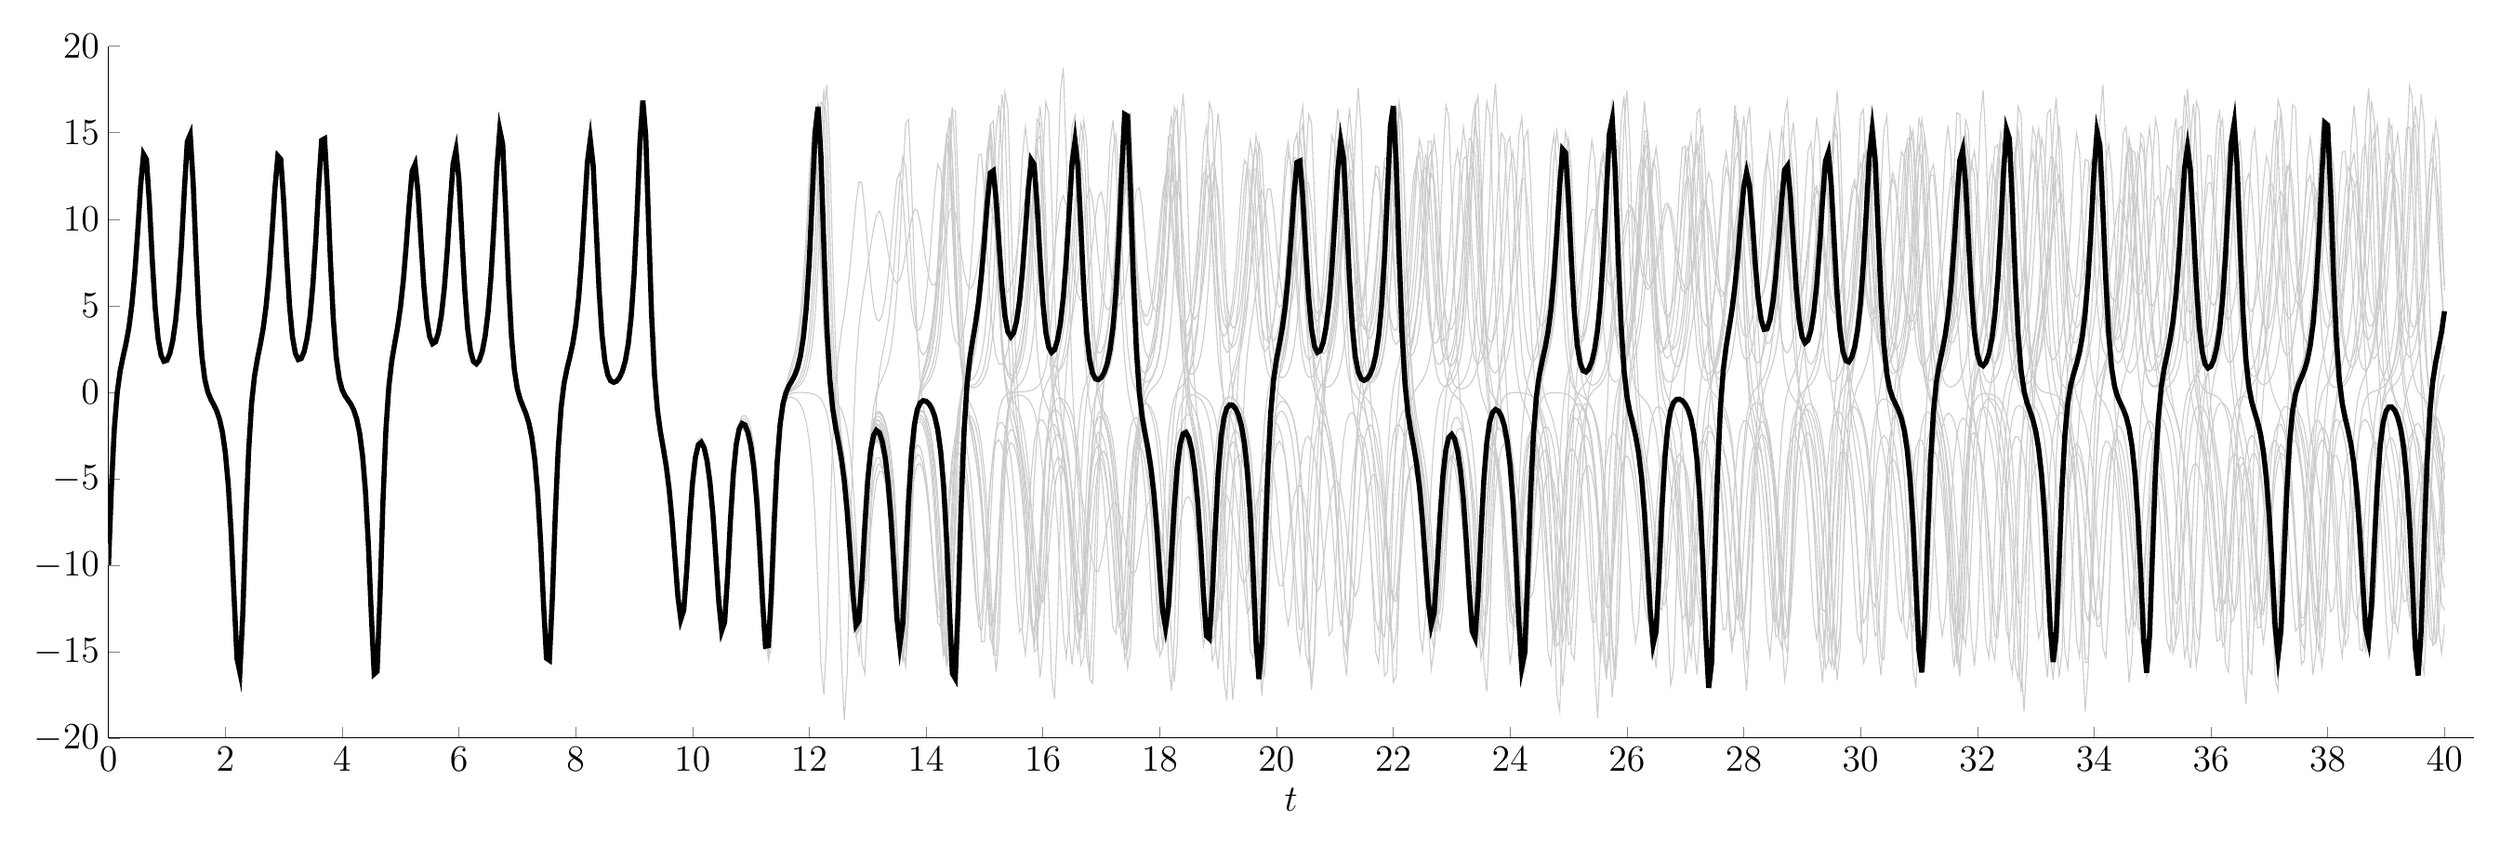
\begin{tikzpicture}

\begin{axis}[%
width=12.72in,
height=3.721in,
at={(2.134in,0.502in)},
scale only axis,
xmin=0,
xmax=40.5,
xlabel={$t$},
xlabel style = {font=\Large},
ymin=-20,
ymax=20,
axis background/.style={fill=white},
axis x line*=bottom,
axis y line*=left,
ticklabel style={font=\Large},legend style={font=\Large},title style={font=\Large}
]
\addplot [color=white!80!black,solid,forget plot]
  table[row sep=crcr]{%
0	-10\\
0.0499775	-5.52917\\
0.099966	-2.11629\\
0.149973	-0.0071032\\
0.19995	1.22622\\
0.249961	2.05059\\
0.299952	2.80706\\
0.349955	3.73834\\
0.399976	5.0388\\
0.449962	6.86782\\
0.499933	9.26983\\
0.549947	11.9128\\
0.599948	13.7536\\
0.649965	13.4628\\
0.699973	10.944\\
0.749983	7.6313\\
0.799972	4.86783\\
0.849964	3.08039\\
0.899953	2.13759\\
0.949959	1.78601\\
0.999971	1.84108\\
1.04995	2.22444\\
1.09997	2.95613\\
1.14997	4.13934\\
1.19998	5.94337\\
1.24996	8.5189\\
1.29995	11.7155\\
1.34994	14.4932\\
1.39994	14.8935\\
1.44993	12.1258\\
1.49995	7.95511\\
1.54996	4.38792\\
1.59998	2.05405\\
1.64998	0.731125\\
1.69998	0.0201058\\
1.74998	-0.392596\\
1.79999	-0.70841\\
1.84999	-1.05761\\
1.90001	-1.54654\\
1.95002	-2.2955\\
2	-3.47264\\
2.04998	-5.3158\\
2.1	-8.09308\\
2.15	-11.8086\\
2.19999	-15.3882\\
2.24999	-16.1964\\
2.3	-12.8261\\
2.34999	-7.66745\\
2.39998	-3.39237\\
2.44998	-0.664123\\
2.5	0.924006\\
2.55001	1.92348\\
2.60002	2.75505\\
2.65	3.7079\\
2.7	5.00002\\
2.75001	6.80294\\
2.80001	9.1692\\
2.85001	11.7865\\
2.9	13.6572\\
2.95	13.4666\\
2.99999	11.0528\\
3.04998	7.78537\\
3.09998	5.01489\\
3.14998	3.20444\\
3.19998	2.24316\\
3.24999	1.88477\\
3.29998	1.94504\\
3.34998	2.34606\\
3.39998	3.10807\\
3.45	4.33669\\
3.49997	6.19497\\
3.55	8.81695\\
3.60001	11.9839\\
3.65003	14.5638\\
3.70002	14.6474\\
3.75	11.7162\\
3.80001	7.62348\\
3.85001	4.22177\\
3.89999	2.02884\\
3.95001	0.799915\\
4	0.154528\\
4.05	-0.200173\\
4.1	-0.44634\\
4.14999	-0.695814\\
4.2	-1.03215\\
4.25001	-1.54394\\
4.3	-2.35457\\
4.35001	-3.65215\\
4.40004	-5.70726\\
4.45005	-8.80466\\
4.50004	-12.8391\\
4.55005	-16.2967\\
4.60007	-16.1377\\
4.65009	-11.7376\\
4.70006	-6.2982\\
4.75008	-2.19928\\
4.80009	0.305794\\
4.85007	1.77908\\
4.90005	2.79139\\
4.95005	3.7479\\
5.00005	4.92113\\
5.05004	6.4971\\
5.10004	8.54999\\
5.15006	10.8846\\
5.20005	12.7885\\
5.25004	13.1714\\
5.30007	11.5592\\
5.35009	8.79767\\
5.40009	6.14458\\
5.45007	4.2583\\
5.50008	3.19993\\
5.5501	2.8042\\
5.6001	2.9122\\
5.6501	3.4523\\
5.70008	4.44574\\
5.75006	5.9811\\
5.80006	8.13802\\
5.85007	10.7827\\
5.90008	13.1927\\
5.95006	13.9871\\
6.00006	12.3123\\
6.05004	9.08617\\
6.10003	5.9268\\
6.15005	3.6736\\
6.20005	2.37097\\
6.25008	1.771\\
6.30006	1.64074\\
6.35006	1.84827\\
6.40008	2.36592\\
6.45008	3.25446\\
6.50008	4.65332\\
6.55006	6.75092\\
6.60006	9.65324\\
6.65003	12.9607\\
6.70002	15.1649\\
6.75003	14.3113\\
6.80003	10.6249\\
6.85004	6.40867\\
6.90007	3.22708\\
6.95006	1.28077\\
7.00006	0.200642\\
7.05005	-0.409352\\
7.10007	-0.831446\\
7.15009	-1.24903\\
7.20009	-1.79874\\
7.25009	-2.61849\\
7.30007	-3.88398\\
7.35008	-5.82839\\
7.40005	-8.6671\\
7.45002	-12.2698\\
7.5	-15.3747\\
7.55	-15.5312\\
7.6	-11.9918\\
7.65	-7.1831\\
7.69999	-3.33579\\
7.75001	-0.910739\\
7.8	0.484312\\
7.85001	1.34311\\
7.90001	2.03474\\
7.95001	2.81511\\
8	3.88673\\
8.04998	5.44196\\
8.09997	7.64882\\
8.14998	10.4833\\
8.19998	13.3065\\
8.24998	14.5843\\
8.29998	13.0443\\
8.34997	9.51194\\
8.39997	5.92332\\
8.44999	3.33382\\
8.5	1.80272\\
8.54999	1.02003\\
8.6	0.685908\\
8.65002	0.608965\\
8.70004	0.696475\\
8.75003	0.926318\\
8.80002	1.3298\\
8.85001	1.99006\\
8.90002	3.05572\\
8.95005	4.75897\\
9.00005	7.39452\\
9.05007	11.1055\\
9.10006	15.1025\\
9.15007	16.7659\\
9.20006	13.8876\\
9.25009	8.47297\\
9.30007	3.71345\\
9.35008	0.608092\\
9.40008	-1.2104\\
9.45009	-2.34999\\
9.50009	-3.28323\\
9.55009	-4.3304\\
9.60009	-5.71191\\
9.65011	-7.56485\\
9.70012	-9.84359\\
9.7501	-12.0883\\
9.80011	-13.2938\\
9.85012	-12.5347\\
9.9001	-10.0945\\
9.95012	-7.23557\\
10.0001	-4.95253\\
10.0501	-3.52767\\
10.1001	-2.85095\\
10.1501	-2.73937\\
10.2001	-3.07598\\
10.2501	-3.84019\\
10.3001	-5.09675\\
10.3501	-6.94963\\
10.4001	-9.41589\\
10.4501	-12.1186\\
10.5001	-13.9416\\
10.5501	-13.505\\
10.6001	-10.8068\\
10.6501	-7.39523\\
10.7001	-4.61464\\
10.7501	-2.84218\\
10.8001	-1.91114\\
10.8501	-1.55327\\
10.9001	-1.57717\\
10.9501	-1.89975\\
11.0001	-2.53258\\
11.0501	-3.56981\\
11.1001	-5.1803\\
11.1501	-7.56109\\
11.2002	-10.7337\\
11.2502	-13.9908\\
11.3002	-15.418\\
11.3502	-13.4189\\
11.4002	-9.18952\\
11.4502	-5.13106\\
11.5002	-2.32749\\
11.5501	-0.68169\\
11.6002	0.236323\\
11.6502	0.802151\\
11.7002	1.2726\\
11.7502	1.8243\\
11.8002	2.6082\\
11.8502	3.7952\\
11.9002	5.60012\\
11.9502	8.23113\\
12.0002	11.6219\\
12.0502	14.7599\\
12.1003	15.446\\
12.1502	12.567\\
12.2002	8.03307\\
12.2502	4.13961\\
12.3002	1.60014\\
12.3502	0.13825\\
12.4002	-0.705557\\
12.4502	-1.29502\\
12.5002	-1.87721\\
12.5502	-2.6363\\
12.6002	-3.74707\\
12.6502	-5.40991\\
12.7002	-7.8174\\
12.7502	-10.9475\\
12.8002	-14.0224\\
12.8502	-15.169\\
12.9002	-13.0375\\
12.9502	-8.92728\\
13.0002	-5.07\\
13.0502	-2.42623\\
13.1002	-0.887545\\
13.1502	-0.0507409\\
13.2002	0.431715\\
13.2501	0.790734\\
13.3002	1.17658\\
13.3501	1.70776\\
13.4001	2.51473\\
13.4501	3.7742\\
13.5001	5.72557\\
13.5501	8.60804\\
13.6001	12.3159\\
13.6502	15.565\\
13.7002	15.7582\\
13.7502	12.0708\\
13.8002	7.08003\\
13.8502	3.11893\\
13.9002	0.635159\\
13.9502	-0.803091\\
14.0002	-1.7137\\
14.0502	-2.48247\\
14.1002	-3.37785\\
14.1502	-4.6104\\
14.2002	-6.36406\\
14.2502	-8.73898\\
14.3002	-11.5149\\
14.3502	-13.7544\\
14.4001	-13.9641\\
14.4501	-11.6542\\
14.5001	-8.17649\\
14.5501	-5.11272\\
14.6001	-3.06503\\
14.6501	-1.93221\\
14.7001	-1.4328\\
14.7501	-1.3399\\
14.8001	-1.53568\\
14.8501	-1.99951\\
14.9002	-2.79333\\
14.9502	-4.05497\\
15.0002	-5.98947\\
15.0502	-8.78295\\
15.1002	-12.2597\\
15.1502	-15.1652\\
15.2002	-15.2186\\
15.2502	-11.8162\\
15.3002	-7.23496\\
15.3502	-3.55131\\
15.4002	-1.22353\\
15.4502	0.104524\\
15.5002	0.890691\\
15.5502	1.47932\\
15.6002	2.10505\\
15.6502	2.95071\\
15.7002	4.19945\\
15.7502	6.05382\\
15.8002	8.67143\\
15.8502	11.8756\\
15.9002	14.5725\\
15.9502	14.8044\\
16.0002	11.9188\\
16.0502	7.75622\\
16.1002	4.25603\\
16.1502	1.98771\\
16.2002	0.708118\\
16.2503	0.0226967\\
16.3003	-0.374283\\
16.3502	-0.678238\\
16.4003	-1.01503\\
16.4502	-1.48685\\
16.5003	-2.21119\\
16.5503	-3.35226\\
16.6002	-5.1446\\
16.6503	-7.86272\\
16.7003	-11.5553\\
16.7503	-15.2504\\
16.8002	-16.3389\\
16.8502	-13.171\\
16.9002	-7.97499\\
16.9502	-3.5689\\
17.0002	-0.730111\\
17.0503	0.925475\\
17.1002	1.95971\\
17.1502	2.80904\\
17.2003	3.77126\\
17.2502	5.06531\\
17.3002	6.86111\\
17.3502	9.20405\\
17.4002	11.7745\\
17.4502	13.5849\\
17.5002	13.3665\\
17.5502	10.9857\\
17.6002	7.78103\\
17.6502	5.06538\\
17.7002	3.29037\\
17.7502	2.35418\\
17.8002	2.02069\\
17.8502	2.11382\\
17.9003	2.56322\\
17.9503	3.39644\\
18.0003	4.7242\\
18.0503	6.70429\\
18.1003	9.42129\\
18.1503	12.5157\\
18.2003	14.6754\\
18.2503	14.1376\\
18.3003	10.9064\\
18.3503	6.96063\\
18.4003	3.85922\\
18.4503	1.92144\\
18.5003	0.864977\\
18.5503	0.335948\\
18.6003	0.0789923\\
18.6503	-0.0550335\\
18.7003	-0.14678\\
18.7503	-0.241628\\
18.8003	-0.37283\\
18.8503	-0.576843\\
18.9003	-0.907068\\
18.9503	-1.45091\\
19.0003	-2.35348\\
19.0503	-3.85078\\
19.1003	-6.29129\\
19.1503	-10.0187\\
19.2003	-14.6924\\
19.2503	-17.7966\\
19.3003	-15.7158\\
19.3503	-9.65574\\
19.4003	-3.86607\\
19.4503	-0.0209161\\
19.5003	2.23084\\
19.5503	3.62591\\
19.6003	4.7316\\
19.6503	5.90006\\
19.7003	7.30959\\
19.7503	8.96545\\
19.8003	10.6218\\
19.8503	11.7437\\
19.9003	11.7402\\
19.9503	10.5062\\
20.0003	8.60278\\
20.0503	6.76948\\
20.1003	5.44874\\
20.1503	4.75277\\
20.2002	4.63318\\
20.2502	5.02339\\
20.3002	5.8901\\
20.3502	7.21886\\
20.4003	8.93101\\
20.4502	10.738\\
20.5002	12.0316\\
20.5502	12.0969\\
20.6002	10.7584\\
20.6502	8.6467\\
20.7002	6.61448\\
20.7503	5.15493\\
20.8003	4.37178\\
20.8503	4.19183\\
20.9003	4.53078\\
20.9503	5.35359\\
21.0003	6.66544\\
21.0503	8.44073\\
21.1003	10.464\\
21.1503	12.1476\\
21.2003	12.621\\
21.2503	11.438\\
21.3003	9.15775\\
21.3503	6.80627\\
21.4003	5.04163\\
21.4503	4.02008\\
21.5003	3.65257\\
21.5503	3.82125\\
21.6003	4.46838\\
21.6503	5.60624\\
21.7003	7.27172\\
21.7502	9.40883\\
21.8003	11.6386\\
21.8502	13.0654\\
21.9002	12.7118\\
21.9502	10.5902\\
22.0002	7.81196\\
22.0502	5.4458\\
22.1002	3.89664\\
22.1502	3.11718\\
22.2002	2.93592\\
22.2502	3.22818\\
22.3002	3.96106\\
22.3502	5.18418\\
22.4002	6.98681\\
22.4502	9.37138\\
22.5002	11.9696\\
22.5502	13.7253\\
22.6003	13.3506\\
22.6503	10.8164\\
22.7003	7.55143\\
22.7502	4.84948\\
22.8002	3.11096\\
22.8502	2.20419\\
22.9003	1.88279\\
22.9503	1.9713\\
23.0003	2.39964\\
23.0503	3.19524\\
23.1003	4.46897\\
23.1502	6.3865\\
23.2002	9.06575\\
23.2502	12.2381\\
23.3002	14.68\\
23.3502	14.502\\
23.4002	11.3932\\
23.4502	7.31113\\
23.5001	4.0076\\
23.5501	1.90819\\
23.6001	0.741715\\
23.6501	0.130633\\
23.7001	-0.207046\\
23.7501	-0.445333\\
23.8001	-0.691491\\
23.8501	-1.02645\\
23.9001	-1.53803\\
23.9501	-2.35019\\
24.0001	-3.65163\\
24.0501	-5.71323\\
24.1001	-8.82494\\
24.1501	-12.8798\\
24.2001	-16.3413\\
24.2501	-16.1485\\
24.3001	-11.7042\\
24.3501	-6.24167\\
24.4002	-2.14183\\
24.4502	0.359937\\
24.5002	1.83327\\
24.5502	2.85047\\
24.6002	3.81605\\
24.6502	5.00253\\
24.7002	6.59292\\
24.7502	8.65156\\
24.8002	10.9653\\
24.8502	12.8045\\
24.9002	13.0973\\
24.9502	11.4329\\
25.0002	8.68586\\
25.0502	6.08291\\
25.1002	4.24601\\
25.1502	3.22743\\
25.2002	2.86285\\
25.2502	2.99952\\
25.3002	3.57191\\
25.3502	4.60652\\
25.4002	6.1905\\
25.4502	8.38783\\
25.5002	11.0237\\
25.5502	13.309\\
25.6003	13.8672\\
25.6502	12.0074\\
25.7003	8.77009\\
25.7503	5.7136\\
25.8003	3.57989\\
25.8503	2.37049\\
25.9003	1.83711\\
25.9503	1.76166\\
26.0003	2.028\\
26.0503	2.62287\\
26.1003	3.62068\\
26.1503	5.17125\\
26.2003	7.4532\\
26.2503	10.4853\\
26.3003	13.6341\\
26.3503	15.1562\\
26.4003	13.4751\\
26.4503	9.52557\\
26.5003	5.57051\\
26.5502	2.76698\\
26.6002	1.10634\\
26.6503	0.203672\\
26.7003	-0.299143\\
26.7503	-0.644544\\
26.8003	-0.986112\\
26.8503	-1.43807\\
26.9003	-2.11655\\
26.9503	-3.17624\\
27.0003	-4.83692\\
27.0503	-7.36514\\
27.1003	-10.8708\\
27.1503	-14.6329\\
27.2003	-16.3201\\
27.2503	-13.8722\\
27.3003	-8.8919\\
27.3502	-4.32402\\
27.4003	-1.2699\\
27.4503	0.52216\\
27.5003	1.60325\\
27.5503	2.425\\
27.6003	3.29965\\
27.6503	4.45606\\
27.7003	6.08212\\
27.7503	8.29576\\
27.8003	10.9519\\
27.8503	13.2889\\
27.9003	13.9232\\
27.9503	12.1089\\
28.0003	8.85816\\
28.0503	5.76041\\
28.1003	3.58533\\
28.1503	2.34453\\
28.2003	1.78829\\
28.2503	1.69122\\
28.3003	1.93144\\
28.3503	2.48952\\
28.4003	3.43448\\
28.4503	4.9129\\
28.5003	7.10948\\
28.5503	10.0908\\
28.6003	13.3385\\
28.6503	15.204\\
28.7003	13.9009\\
28.7503	10.0414\\
28.8003	5.94418\\
28.8503	2.95881\\
28.9003	1.16301\\
28.9503	0.175944\\
29.0003	-0.380991\\
29.0503	-0.769582\\
29.1003	-1.1596\\
29.1503	-1.67768\\
29.2003	-2.45449\\
29.2504	-3.66127\\
29.3003	-5.52761\\
29.3504	-8.29617\\
29.4004	-11.9138\\
29.4504	-15.2618\\
29.5004	-15.8438\\
29.5504	-12.5207\\
29.6004	-7.59569\\
29.6504	-3.53123\\
29.7003	-0.936045\\
29.7503	0.566104\\
29.8004	1.49116\\
29.8503	2.2323\\
29.9003	3.06272\\
29.9504	4.19477\\
30.0004	5.81851\\
30.0504	8.0753\\
30.1004	10.8685\\
30.1504	13.4516\\
30.2004	14.3065\\
30.2504	12.4784\\
30.3003	9.00621\\
30.3503	5.66249\\
30.4003	3.31274\\
30.4503	1.95459\\
30.5003	1.29814\\
30.5503	1.07981\\
30.6004	1.14365\\
30.6504	1.43329\\
30.7004	1.97182\\
30.7504	2.85301\\
30.8004	4.24715\\
30.8504	6.38905\\
30.9004	9.46447\\
30.9504	13.1585\\
31.0004	15.8273\\
31.0504	15.0278\\
31.1004	10.8632\\
31.1504	6.1044\\
31.2003	2.57609\\
31.2503	0.427011\\
31.3003	-0.812528\\
31.3503	-1.61938\\
31.4003	-2.33654\\
31.4503	-3.20519\\
31.5003	-4.42509\\
31.5503	-6.18531\\
31.6003	-8.60849\\
31.6503	-11.5071\\
31.7003	-13.9339\\
31.7503	-14.2644\\
31.8003	-11.878\\
31.8503	-8.20742\\
31.9003	-4.97353\\
31.9503	-2.81293\\
32.0003	-1.60486\\
32.0503	-1.03214\\
32.1003	-0.841096\\
32.1503	-0.887693\\
32.2003	-1.11965\\
32.2503	-1.5545\\
32.3003	-2.27195\\
32.3503	-3.41999\\
32.4003	-5.22862\\
32.4503	-7.96125\\
32.5003	-11.6453\\
32.5503	-15.2699\\
32.6003	-16.2407\\
32.6503	-13.0199\\
32.7003	-7.87702\\
32.7503	-3.5454\\
32.8003	-0.760402\\
32.8503	0.861489\\
32.9003	1.87412\\
32.9503	2.70346\\
33.0003	3.64319\\
33.0503	4.91276\\
33.1003	6.68754\\
33.1503	9.03082\\
33.2003	11.6607\\
33.2503	13.6123\\
33.3003	13.5519\\
33.3503	11.2205\\
33.4003	7.94745\\
33.4503	5.12486\\
33.5003	3.26075\\
33.5503	2.25888\\
33.6003	1.87203\\
33.6503	1.90919\\
33.7003	2.28612\\
33.7503	3.01776\\
33.8003	4.20395\\
33.8503	6.00812\\
33.9003	8.57266\\
33.9503	11.732\\
34.0003	14.4418\\
34.0502	14.79\\
34.1002	12.0436\\
34.1503	7.93921\\
34.2003	4.43275\\
34.2502	2.13837\\
34.3002	0.841265\\
34.3502	0.155364\\
34.4002	-0.223657\\
34.4502	-0.487713\\
34.5002	-0.755822\\
34.5502	-1.11709\\
34.6002	-1.66593\\
34.6502	-2.53336\\
34.7002	-3.91629\\
34.7502	-6.08873\\
34.8002	-9.3121\\
34.8502	-13.3539\\
34.9002	-16.4532\\
34.9502	-15.6684\\
35.0002	-10.9975\\
35.0502	-5.72508\\
35.1002	-1.89453\\
35.1502	0.41818\\
35.2002	1.78625\\
35.2502	2.75277\\
35.3002	3.69818\\
35.3502	4.88228\\
35.4002	6.48961\\
35.4502	8.59547\\
35.5002	10.9951\\
35.5502	12.9426\\
35.6002	13.2899\\
35.6503	11.5649\\
35.7002	8.69323\\
35.7503	5.97758\\
35.8003	4.07034\\
35.8503	3.0068\\
35.9003	2.60345\\
35.9503	2.69187\\
36.0003	3.19619\\
36.0503	4.13677\\
36.1003	5.60905\\
36.1503	7.71917\\
36.2003	10.4025\\
36.2503	13.0399\\
36.3003	14.2335\\
36.3503	12.8456\\
36.4003	9.58913\\
36.4503	6.20871\\
36.5003	3.72954\\
36.5503	2.25577\\
36.6003	1.52976\\
36.6503	1.28598\\
36.7003	1.36033\\
36.7502	1.69251\\
36.8002	2.30846\\
36.8502	3.3114\\
36.9002	4.8788\\
36.9502	7.23325\\
37.0002	10.4581\\
37.0502	13.9426\\
37.1002	15.739\\
37.1502	13.9182\\
37.2002	9.52732\\
37.2502	5.19529\\
37.3002	2.17175\\
37.3502	0.38262\\
37.4002	-0.641142\\
37.4502	-1.31546\\
37.5002	-1.93016\\
37.5502	-2.69229\\
37.6002	-3.78518\\
37.6502	-5.40371\\
37.7002	-7.73256\\
37.7502	-10.7502\\
37.8002	-13.7408\\
37.8502	-14.9641\\
37.9002	-13.0783\\
37.9502	-9.18291\\
38.0002	-5.40943\\
38.0502	-2.77404\\
38.1003	-1.23102\\
38.1503	-0.412276\\
38.2003	0.0141002\\
38.2503	0.265835\\
38.3003	0.471711\\
38.3503	0.714924\\
38.4003	1.06764\\
38.4503	1.61936\\
38.5003	2.5038\\
38.5503	3.92839\\
38.6003	6.1865\\
38.6503	9.5528\\
38.7003	13.7556\\
38.7503	16.8228\\
38.8003	15.6528\\
38.8503	10.5921\\
38.9003	5.18664\\
38.9504	1.37418\\
39.0004	-0.9022\\
39.0504	-2.26733\\
39.1004	-3.27503\\
39.1504	-4.30219\\
39.2004	-5.59815\\
39.2503	-7.31061\\
39.3004	-9.42767\\
39.3504	-11.5862\\
39.4004	-12.9288\\
39.4504	-12.55\\
39.5003	-10.4932\\
39.5503	-7.81698\\
39.6003	-5.53569\\
39.6503	-4.04278\\
39.7003	-3.30127\\
39.7504	-3.15521\\
39.8004	-3.49104\\
39.8503	-4.28145\\
39.9004	-5.57618\\
39.9504	-7.44412\\
40.0003	-9.82945\\
};
\addplot [color=white!80!black,solid,forget plot]
  table[row sep=crcr]{%
0	-10\\
0.0500142	-5.52615\\
0.100006	-2.11411\\
0.150003	-0.00615096\\
0.200011	1.22739\\
0.25001	2.05132\\
0.299996	2.80776\\
0.350018	3.73968\\
0.400019	5.04012\\
0.450023	6.87041\\
0.500015	9.27412\\
0.549996	11.9152\\
0.599972	13.7541\\
0.649968	13.4627\\
0.699967	10.9445\\
0.749962	7.63271\\
0.799946	4.86908\\
0.849926	3.08142\\
0.899919	2.13801\\
0.949913	1.78612\\
0.999897	1.84073\\
1.0499	2.22383\\
1.0999	2.95477\\
1.1499	4.13734\\
1.19989	5.93963\\
1.24988	8.51399\\
1.29987	11.7102\\
1.34986	14.4901\\
1.39988	14.8951\\
1.44987	12.1303\\
1.49988	7.96144\\
1.54985	4.39456\\
1.59984	2.05877\\
1.64984	0.733735\\
1.69983	0.0216172\\
1.74983	-0.391663\\
1.79984	-0.707537\\
1.84982	-1.05637\\
1.89982	-1.54436\\
1.94983	-2.29213\\
1.99983	-3.46796\\
2.04984	-5.30939\\
2.09984	-8.0828\\
2.14985	-11.7969\\
2.19985	-15.3809\\
2.24987	-16.1995\\
2.29987	-12.8385\\
2.34988	-7.6782\\
2.39989	-3.39892\\
2.44991	-0.666838\\
2.49991	0.921862\\
2.54992	1.9219\\
2.5999	2.75306\\
2.6499	3.7056\\
2.69988	4.99646\\
2.74988	6.79779\\
2.79988	9.16252\\
2.84985	11.779\\
2.89986	13.6545\\
2.94987	13.4704\\
2.99985	11.0618\\
3.04983	7.79493\\
3.09983	5.02172\\
3.14982	3.20845\\
3.19983	2.2449\\
3.24983	1.88501\\
3.29984	1.94423\\
3.34986	2.34442\\
3.39988	3.10582\\
3.44987	4.33238\\
3.49988	6.19036\\
3.54988	8.80909\\
3.59987	11.9746\\
3.64989	14.5591\\
3.69991	14.6515\\
3.7499	11.7253\\
3.79991	7.63227\\
3.84994	4.22603\\
3.89995	2.0304\\
3.94993	0.801258\\
3.99991	0.155104\\
4.04992	-0.200016\\
4.09992	-0.446392\\
4.14991	-0.695938\\
4.19992	-1.03228\\
4.24993	-1.54421\\
4.29993	-2.35483\\
4.34991	-3.65155\\
4.39989	-5.70411\\
4.44989	-8.79875\\
4.49989	-12.8333\\
4.54989	-16.2923\\
4.59988	-16.1429\\
4.64986	-11.754\\
4.69988	-6.30899\\
4.74987	-2.20869\\
4.79991	0.300821\\
4.84989	1.77543\\
4.89989	2.78846\\
4.94986	3.74403\\
4.99984	4.91594\\
5.04985	6.49113\\
5.09986	8.54326\\
5.14988	10.8787\\
5.19987	12.7858\\
5.24988	13.1742\\
5.29986	11.568\\
5.34988	8.80774\\
5.39988	6.15163\\
5.44988	4.26185\\
5.49985	3.20124\\
5.54984	2.80317\\
5.59983	2.90882\\
5.64984	3.44679\\
5.69987	4.4386\\
5.74986	5.97144\\
5.79987	8.12676\\
5.84989	10.7717\\
5.8999	13.186\\
5.9499	13.9905\\
5.99989	12.3249\\
6.0499	9.09816\\
6.09992	5.93348\\
6.1499	3.67825\\
6.19989	2.3724\\
6.24989	1.77011\\
6.29988	1.63765\\
6.34988	1.84312\\
6.39989	2.35815\\
6.44988	3.24292\\
6.49989	4.63683\\
6.54988	6.7285\\
6.59989	9.62619\\
6.64989	12.9384\\
6.69988	15.1611\\
6.74989	14.3335\\
6.7999	10.6578\\
6.84989	6.43638\\
6.8999	3.24418\\
6.94989	1.28849\\
6.99989	0.202367\\
7.04988	-0.411014\\
7.09986	-0.834923\\
7.14986	-1.25393\\
7.19985	-1.80517\\
7.24983	-2.62655\\
7.29983	-3.89515\\
7.34983	-5.84215\\
7.39984	-8.68655\\
7.44985	-12.29\\
7.49985	-15.3803\\
7.54985	-15.5106\\
7.59984	-11.9597\\
7.64982	-7.16062\\
7.69984	-3.32426\\
7.74982	-0.91072\\
7.79982	0.478425\\
7.84984	1.33351\\
7.89986	2.02221\\
7.94986	2.79935\\
7.99985	3.86689\\
8.04985	5.4183\\
8.09986	7.62261\\
8.14988	10.4586\\
8.19989	13.2962\\
8.2499	14.5997\\
8.29989	13.0784\\
8.34989	9.54268\\
8.39992	5.93692\\
8.44991	3.33485\\
8.49989	1.79363\\
8.54992	1.00269\\
8.59991	0.661771\\
8.64991	0.576359\\
8.69992	0.651591\\
8.74993	0.862764\\
8.79993	1.23702\\
8.84993	1.85117\\
8.89994	2.8444\\
8.94995	4.43724\\
8.99993	6.92473\\
9.04993	10.5104\\
9.09993	14.6206\\
9.14993	16.8561\\
9.19993	14.5915\\
9.24995	9.2601\\
9.29996	4.24976\\
9.34997	0.891767\\
9.39998	-1.08501\\
9.44996	-2.29893\\
9.49997	-3.25261\\
9.54996	-4.28513\\
9.59995	-5.62735\\
9.64994	-7.42198\\
9.69996	-9.64363\\
9.74996	-11.8779\\
9.79996	-13.1769\\
9.84997	-12.5991\\
9.89999	-10.3058\\
9.94996	-7.49464\\
9.99996	-5.18396\\
10.05	-3.71204\\
10.1	-2.99647\\
10.15	-2.86095\\
10.2	-3.18644\\
10.25	-3.94851\\
10.3	-5.20514\\
10.35	-7.04998\\
10.4	-9.48487\\
10.45	-12.1165\\
10.5	-13.8396\\
10.55	-13.351\\
10.6	-10.6986\\
10.65	-7.37947\\
10.7	-4.67936\\
10.75	-2.96068\\
10.8	-2.06908\\
10.85	-1.75032\\
10.9	-1.82623\\
10.95	-2.22564\\
11	-2.97339\\
11.05	-4.17814\\
11.1	-6.0114\\
11.15	-8.62454\\
11.1999	-11.8468\\
11.25	-14.5924\\
11.3	-14.8742\\
11.35	-11.9881\\
11.4	-7.78685\\
11.45	-4.24726\\
11.5	-1.94978\\
11.55	-0.650584\\
11.6	0.0515661\\
11.65	0.469526\\
11.7	0.803664\\
11.75	1.1866\\
11.8	1.73093\\
11.85	2.56668\\
11.9	3.87764\\
11.95	5.91256\\
12	8.90795\\
12.05	12.7011\\
12.1	15.8404\\
12.15	15.6532\\
12.2	11.6371\\
12.25	6.59695\\
12.3	2.731\\
12.35	0.342922\\
12.4	-1.04423\\
12.45	-1.95015\\
12.5	-2.7543\\
12.55	-3.72123\\
12.6	-5.05888\\
12.65	-6.93619\\
12.7	-9.39658\\
12.75	-12.0816\\
12.8	-13.891\\
12.85	-13.4696\\
12.9	-10.8089\\
12.95	-7.43022\\
13	-4.66555\\
13.05	-2.90168\\
13.1	-1.9767\\
13.15	-1.62752\\
13.2	-1.66649\\
13.25	-2.01373\\
13.3	-2.68459\\
13.35	-3.77802\\
13.4	-5.4648\\
13.45	-7.92827\\
13.4999	-11.1294\\
13.5499	-14.2329\\
13.5999	-15.2683\\
13.6499	-12.9308\\
13.6999	-8.68607\\
13.7499	-4.80777\\
13.7999	-2.18756\\
13.8499	-0.669822\\
13.8999	0.168503\\
13.9499	0.680592\\
13.9999	1.1027\\
14.0499	1.59522\\
14.0999	2.29649\\
14.1499	3.36493\\
14.1999	5.00878\\
14.2499	7.46715\\
14.2999	10.8025\\
14.3499	14.2978\\
14.3999	15.8494\\
14.4499	13.641\\
14.4999	9.05559\\
14.5499	4.75063\\
14.5999	1.82475\\
14.6499	0.108609\\
14.6999	-0.888253\\
14.7499	-1.58019\\
14.7999	-2.25397\\
14.8499	-3.11987\\
14.8999	-4.36826\\
14.95	-6.19433\\
14.9999	-8.7295\\
15.05	-11.774\\
15.1	-14.2786\\
15.15	-14.47\\
15.2	-11.7833\\
15.25	-7.88317\\
15.3	-4.55865\\
15.35	-2.38548\\
15.3999	-1.17137\\
15.4499	-0.564298\\
15.4999	-0.290412\\
15.5499	-0.186266\\
15.5999	-0.16927\\
15.6499	-0.20555\\
15.6999	-0.289679\\
15.7499	-0.435986\\
15.7999	-0.678605\\
15.8499	-1.07986\\
15.8999	-1.7469\\
15.9499	-2.85953\\
15.9999	-4.70512\\
16.0499	-7.66892\\
16.0999	-11.9597\\
16.1499	-16.5007\\
16.1999	-17.7345\\
16.2499	-13.4195\\
16.2999	-6.97777\\
16.3499	-1.92061\\
16.3999	1.18855\\
16.4499	3.00811\\
16.4999	4.23374\\
16.5498	5.33847\\
16.5998	6.59273\\
16.6498	8.09721\\
16.6998	9.7507\\
16.7498	11.1758\\
16.7998	11.7873\\
16.8498	11.1903\\
16.8998	9.61025\\
16.9498	7.73393\\
16.9998	6.16532\\
17.0498	5.17147\\
17.0998	4.77438\\
17.1498	4.91329\\
17.1998	5.53794\\
17.2498	6.62547\\
17.2998	8.13354\\
17.3498	9.88808\\
17.3998	11.4432\\
17.4498	12.1107\\
17.4998	11.4202\\
17.5498	9.64024\\
17.5998	7.56839\\
17.6498	5.87221\\
17.6998	4.81162\\
17.7498	4.38307\\
17.7998	4.50383\\
17.8498	5.11755\\
17.8998	6.21134\\
17.9498	7.77217\\
17.9998	9.6721\\
18.0498	11.4918\\
18.0998	12.4631\\
18.1498	11.9235\\
18.1998	10.044\\
18.2498	7.7232\\
18.2998	5.77247\\
18.3498	4.5157\\
18.3998	3.94132\\
18.4498	3.94051\\
18.4997	4.43558\\
18.5497	5.41381\\
18.5997	6.90014\\
18.6497	8.86262\\
18.6997	11.0231\\
18.7497	12.6506\\
18.7997	12.7793\\
18.8497	11.1291\\
18.8997	8.54741\\
18.9497	6.13144\\
18.9997	4.4406\\
19.0497	3.52431\\
19.0997	3.24274\\
19.1497	3.46857\\
19.1997	4.15375\\
19.2497	5.32834\\
19.2997	7.05897\\
19.3497	9.32627\\
19.3997	11.7675\\
19.4497	13.4144\\
19.4997	13.1085\\
19.5497	10.7993\\
19.5997	7.74968\\
19.6497	5.17264\\
19.6997	3.49267\\
19.7497	2.6239\\
19.7997	2.35415\\
19.8497	2.52884\\
19.8997	3.09466\\
19.9497	4.09383\\
19.9997	5.64148\\
20.0497	7.85787\\
20.0997	10.6721\\
20.1497	13.386\\
20.1997	14.4647\\
20.2497	12.781\\
20.2997	9.26921\\
20.3497	5.79342\\
20.3997	3.31851\\
20.4497	1.86928\\
20.4997	1.1453\\
20.5497	0.864221\\
20.5997	0.850919\\
20.6497	1.02947\\
20.6996	1.39867\\
20.7496	2.01998\\
20.7996	3.02039\\
20.8496	4.60464\\
20.8996	7.04048\\
20.9496	10.4774\\
20.9996	14.3323\\
21.0496	16.398\\
21.0996	14.3378\\
21.1497	9.40196\\
21.1997	4.66238\\
21.2496	1.43276\\
21.2996	-0.474515\\
21.3496	-1.61661\\
21.3996	-2.46593\\
21.4496	-3.34995\\
21.4996	-4.50381\\
21.5496	-6.11736\\
21.5996	-8.30088\\
21.6496	-10.9083\\
21.6996	-13.1932\\
21.7496	-13.8198\\
21.7996	-12.0652\\
21.8496	-8.89864\\
21.8996	-5.8592\\
21.9496	-3.71256\\
21.9996	-2.48668\\
22.0496	-1.94603\\
22.0996	-1.87518\\
22.1496	-2.15914\\
22.1996	-2.78567\\
22.2495	-3.83165\\
22.2995	-5.44726\\
22.3496	-7.79585\\
22.3996	-10.8434\\
22.4496	-13.8401\\
22.4996	-15.0062\\
22.5496	-13.0213\\
22.5996	-9.06522\\
22.6496	-5.2862\\
22.6996	-2.66627\\
22.7496	-1.13825\\
22.7996	-0.323353\\
22.8496	0.11167\\
22.8996	0.385743\\
22.9496	0.631524\\
22.9995	0.939906\\
23.0495	1.397\\
23.0995	2.11454\\
23.1495	3.26064\\
23.1996	5.0826\\
23.2496	7.87601\\
23.2996	11.7139\\
23.3496	15.5688\\
23.3996	16.6227\\
23.4496	13.156\\
23.4996	7.68857\\
23.5496	3.16159\\
23.5996	0.28494\\
23.6496	-1.39646\\
23.6996	-2.47907\\
23.7496	-3.41045\\
23.7996	-4.49213\\
23.8496	-5.93391\\
23.8996	-7.8558\\
23.9496	-10.1746\\
23.9996	-12.3522\\
24.0496	-13.3267\\
24.0996	-12.2816\\
24.1496	-9.69462\\
24.1996	-6.86771\\
24.2496	-4.69399\\
24.2996	-3.38043\\
24.3496	-2.79055\\
24.3996	-2.74375\\
24.4496	-3.13557\\
24.4996	-3.95816\\
24.5496	-5.28587\\
24.5997	-7.22243\\
24.6497	-9.75735\\
24.6997	-12.4365\\
24.7497	-14.0468\\
24.7997	-13.2824\\
24.8497	-10.385\\
24.8997	-6.98762\\
24.9497	-4.32178\\
24.9997	-2.66515\\
25.0497	-1.81718\\
25.0997	-1.51181\\
25.1497	-1.56972\\
25.1997	-1.91933\\
25.2497	-2.58137\\
25.2997	-3.65807\\
25.3497	-5.32509\\
25.3997	-7.77839\\
25.4497	-11.0113\\
25.4997	-14.2266\\
25.5497	-15.4236\\
25.5997	-13.1495\\
25.6497	-8.82645\\
25.6997	-4.83058\\
25.7497	-2.12061\\
25.7997	-0.542617\\
25.8496	0.341527\\
25.8996	0.902345\\
25.9496	1.39071\\
25.9996	1.98201\\
26.0496	2.8317\\
26.0996	4.11819\\
26.1496	6.05972\\
26.1996	8.83854\\
26.2496	12.2631\\
26.2996	15.0792\\
26.3496	15.084\\
26.3996	11.7342\\
26.4495	7.2485\\
26.4995	3.63594\\
26.5495	1.35031\\
26.5995	0.0520269\\
26.6495	-0.702588\\
26.6995	-1.2461\\
26.7495	-1.80392\\
26.7995	-2.54636\\
26.8495	-3.64499\\
26.8995	-5.30234\\
26.9495	-7.7201\\
26.9995	-10.8989\\
27.0495	-14.0807\\
27.0995	-15.336\\
27.1495	-13.1978\\
27.1995	-8.97731\\
27.2495	-5.0093\\
27.2995	-2.29269\\
27.3495	-0.706106\\
27.3995	0.172487\\
27.4495	0.707964\\
27.4995	1.14625\\
27.5495	1.65434\\
27.5995	2.37517\\
27.6495	3.47083\\
27.6995	5.15071\\
27.7495	7.64645\\
27.7995	10.9909\\
27.8495	14.4044\\
27.8995	15.7514\\
27.9495	13.386\\
27.9995	8.82171\\
28.0495	4.6231\\
28.0995	1.79514\\
28.1495	0.143084\\
28.1995	-0.812585\\
28.2495	-1.47386\\
28.2996	-2.11656\\
28.3496	-2.94331\\
28.3996	-4.14043\\
28.4496	-5.90502\\
28.4996	-8.39472\\
28.5496	-11.4772\\
28.5995	-14.2005\\
28.6495	-14.7389\\
28.6995	-12.2402\\
28.7495	-8.25923\\
28.7995	-4.74872\\
28.8496	-2.41068\\
28.8995	-1.08385\\
28.9496	-0.395648\\
28.9996	-0.0484692\\
29.0496	0.1452\\
29.0996	0.291839\\
29.1496	0.45615\\
29.1996	0.690158\\
29.2496	1.0558\\
29.2996	1.64567\\
29.3496	2.60794\\
29.3996	4.17794\\
29.4496	6.68542\\
29.4996	10.3988\\
29.5496	14.8236\\
29.5996	17.3962\\
29.6496	15.0389\\
29.6996	9.26556\\
29.7496	3.88855\\
29.7996	0.327188\\
29.8496	-1.76478\\
29.8996	-3.06938\\
29.9496	-4.12096\\
29.9996	-5.26532\\
30.0496	-6.70605\\
30.0996	-8.5035\\
30.1496	-10.4757\\
30.1996	-12.0568\\
30.2496	-12.4404\\
30.2997	-11.2527\\
30.3496	-9.05782\\
30.3996	-6.81594\\
30.4496	-5.14011\\
30.4996	-4.18066\\
30.5497	-3.86054\\
30.5997	-4.07412\\
30.6497	-4.77068\\
30.6997	-5.95993\\
30.7497	-7.66146\\
30.7996	-9.76859\\
30.8496	-11.8311\\
30.8996	-12.9443\\
30.9496	-12.2942\\
30.9996	-10.1017\\
31.0496	-7.46815\\
31.0997	-5.315\\
31.1497	-3.95321\\
31.1997	-3.31809\\
31.2497	-3.25726\\
31.2997	-3.67214\\
31.3497	-4.54974\\
31.3997	-5.94425\\
31.4497	-7.91109\\
31.4997	-10.3325\\
31.5497	-12.6158\\
31.5997	-13.5885\\
31.6497	-12.3794\\
31.6997	-9.57438\\
31.7497	-6.59915\\
31.7997	-4.364\\
31.8497	-3.03089\\
31.8997	-2.4245\\
31.9497	-2.34194\\
31.9997	-2.66729\\
32.0497	-3.38686\\
32.0997	-4.57545\\
32.1497	-6.36356\\
32.1997	-8.83994\\
32.2497	-11.7631\\
32.2997	-14.0964\\
32.3497	-14.1967\\
32.3997	-11.6066\\
32.4497	-7.89168\\
32.4997	-4.71838\\
32.5497	-2.63832\\
32.5997	-1.4885\\
32.6497	-0.94809\\
32.6997	-0.768598\\
32.7497	-0.811372\\
32.7997	-1.02651\\
32.8497	-1.43012\\
32.8997	-2.09711\\
32.9497	-3.16912\\
32.9997	-4.86747\\
33.0497	-7.4692\\
33.0997	-11.0809\\
33.1497	-14.9163\\
33.1997	-16.4871\\
33.2497	-13.7512\\
33.2997	-8.57205\\
33.3497	-3.96446\\
33.3997	-0.935907\\
33.4497	0.837658\\
33.4997	1.92977\\
33.5497	2.79581\\
33.5997	3.75051\\
33.6497	5.01938\\
33.6997	6.77417\\
33.7497	9.06711\\
33.7997	11.6068\\
33.8497	13.4594\\
33.8997	13.373\\
33.9497	11.1303\\
33.9997	7.98369\\
34.0497	5.25702\\
34.0997	3.44945\\
34.1497	2.48642\\
34.1996	2.13901\\
34.2497	2.23276\\
34.2997	2.69612\\
34.3497	3.55594\\
34.3997	4.92053\\
34.4497	6.93999\\
34.4997	9.66754\\
34.5497	12.6817\\
34.5997	14.6235\\
34.6497	13.8523\\
34.6997	10.5738\\
34.7497	6.74739\\
34.7997	3.79337\\
34.8497	1.96778\\
34.8997	0.988546\\
34.9497	0.521766\\
34.9997	0.332133\\
35.0497	0.289913\\
35.0997	0.337006\\
35.1497	0.460105\\
35.1996	0.676947\\
35.2497	1.03579\\
35.2997	1.62445\\
35.3497	2.59259\\
35.3997	4.17985\\
35.4497	6.72516\\
35.4997	10.5075\\
35.5497	15.0012\\
35.5997	17.5365\\
35.6497	14.9923\\
35.6997	9.0697\\
35.7496	3.65399\\
35.7996	0.100851\\
35.8496	-1.98164\\
35.8996	-3.28935\\
35.9496	-4.35688\\
35.9996	-5.52307\\
36.0496	-6.97851\\
36.0996	-8.75678\\
36.1496	-10.6365\\
36.1996	-12.0336\\
36.2496	-12.2075\\
36.2996	-10.9212\\
36.3496	-8.78428\\
36.3996	-6.68598\\
36.4496	-5.15588\\
36.4996	-4.3146\\
36.5496	-4.08758\\
36.5996	-4.3843\\
36.6496	-5.16511\\
36.6996	-6.43746\\
36.7496	-8.19107\\
36.7996	-10.2505\\
36.8496	-12.0664\\
36.8996	-12.7453\\
36.9496	-11.7174\\
36.9996	-9.45035\\
37.0496	-7.00458\\
37.0996	-5.11956\\
37.1496	-3.99375\\
37.1996	-3.54297\\
37.2496	-3.63913\\
37.2996	-4.21278\\
37.3496	-5.26912\\
37.3996	-6.85591\\
37.4496	-8.95951\\
37.4996	-11.2855\\
37.5496	-13.0148\\
37.5996	-13.0563\\
37.6495	-11.1482\\
37.6996	-8.30953\\
37.7495	-5.74783\\
37.7995	-3.99991\\
37.8495	-3.06229\\
37.8995	-2.7561\\
37.9495	-2.93303\\
37.9995	-3.53715\\
38.0495	-4.60334\\
38.0995	-6.22769\\
38.1495	-8.47928\\
38.1995	-11.1678\\
38.2495	-13.4621\\
38.2995	-13.9358\\
38.3495	-11.9373\\
38.3995	-8.60424\\
38.4495	-5.52475\\
38.4995	-3.40212\\
38.5495	-2.20653\\
38.5995	-1.67725\\
38.6495	-1.58879\\
38.6995	-1.82238\\
38.7494	-2.36015\\
38.7995	-3.27142\\
38.8495	-4.70248\\
38.8994	-6.84711\\
38.9495	-9.80768\\
38.9994	-13.1464\\
39.0494	-15.2747\\
39.0994	-14.2406\\
39.1494	-10.4171\\
39.1995	-6.179\\
39.2495	-3.03414\\
39.2995	-1.12361\\
39.3495	-0.0613544\\
39.3995	0.553175\\
39.4495	1.00185\\
39.4995	1.47147\\
39.5495	2.1066\\
39.5995	3.05933\\
39.6495	4.52254\\
39.6995	6.72982\\
39.7495	9.82509\\
39.7995	13.3886\\
39.8495	15.6933\\
39.8995	14.5389\\
39.9495	10.3734\\
39.9995	5.85784\\
};
\addplot [color=white!80!black,solid,forget plot]
  table[row sep=crcr]{%
0	-10\\
0.0499995	-5.52736\\
0.099992	-2.11488\\
0.149975	-0.007029\\
0.199972	1.22665\\
0.249969	2.05071\\
0.299944	2.80693\\
0.349922	3.73762\\
0.399925	5.03723\\
0.449932	6.86652\\
0.499942	9.27027\\
0.549959	11.9134\\
0.599974	13.7541\\
0.649961	13.4629\\
0.699962	10.9448\\
0.749961	7.63276\\
0.799977	4.86759\\
0.849965	3.08035\\
0.899967	2.13741\\
0.949942	1.78603\\
0.999942	1.84093\\
1.04995	2.22436\\
1.09994	2.95557\\
1.14993	4.13824\\
1.19992	5.94095\\
1.24991	8.51603\\
1.2999	11.7119\\
1.3499	14.4918\\
1.39993	14.8936\\
1.44994	12.125\\
1.49994	7.95656\\
1.54994	4.38886\\
1.59994	2.05533\\
1.64996	0.731533\\
1.69995	0.0203785\\
1.74994	-0.392428\\
1.79993	-0.708125\\
1.84993	-1.05723\\
1.89992	-1.54564\\
1.94993	-2.29417\\
1.99994	-3.47105\\
2.04997	-5.31545\\
2.09996	-8.09093\\
2.14995	-11.8053\\
2.19996	-15.3871\\
2.24996	-16.1969\\
2.29995	-12.8306\\
2.34994	-7.67145\\
2.39996	-3.39368\\
2.44997	-0.664422\\
2.49995	0.922728\\
2.54995	1.92243\\
2.59995	2.75384\\
2.64998	3.70733\\
2.69997	4.99909\\
2.74994	6.80029\\
2.79995	9.16625\\
2.84994	11.7835\\
2.89995	13.6563\\
2.94995	13.4681\\
2.99995	11.0554\\
3.04994	7.78781\\
3.09993	5.01684\\
3.14995	3.20484\\
3.19994	2.24343\\
3.24994	1.88464\\
3.29995	1.94463\\
3.34993	2.34512\\
3.39991	3.10631\\
3.44989	4.33286\\
3.49991	6.19136\\
3.5499	8.81023\\
3.59991	11.9771\\
3.64994	14.5607\\
3.69996	14.6502\\
3.74996	11.7206\\
3.79997	7.62798\\
3.84996	4.22494\\
3.89995	2.03032\\
3.94995	0.800804\\
3.99996	0.154508\\
4.04997	-0.20053\\
4.09997	-0.446867\\
4.14999	-0.696783\\
4.19997	-1.03321\\
4.24995	-1.54527\\
4.29997	-2.35701\\
4.34999	-3.65594\\
4.39996	-5.71024\\
4.44997	-8.80764\\
4.49997	-12.844\\
4.54996	-16.2972\\
4.59995	-16.136\\
4.64994	-11.7396\\
4.69992	-6.30037\\
4.74991	-2.20364\\
4.79992	0.302458\\
4.8499	1.77627\\
4.8999	2.78887\\
4.9499	3.74503\\
4.9999	4.91766\\
5.04989	6.49291\\
5.09987	8.54484\\
5.14985	10.8786\\
5.19986	12.7865\\
5.24983	13.1751\\
5.29984	11.5686\\
5.34985	8.80774\\
5.39983	6.15233\\
5.44985	4.26104\\
5.49986	3.19995\\
5.54986	2.80213\\
5.59986	2.90811\\
5.64984	3.4458\\
5.69983	4.4367\\
5.74981	5.96878\\
5.79983	8.12389\\
5.84984	10.7681\\
5.89982	13.1832\\
5.94984	13.992\\
5.99983	12.329\\
6.04982	9.10466\\
6.09983	5.93891\\
6.14981	3.68086\\
6.1998	2.37307\\
6.24978	1.76953\\
6.29979	1.63592\\
6.3498	1.84042\\
6.39978	2.35383\\
6.44976	3.23624\\
6.49975	4.62649\\
6.54975	6.7147\\
6.59976	9.60932\\
6.64975	12.9223\\
6.69976	15.1581\\
6.74975	14.3492\\
6.79973	10.6842\\
6.84974	6.45699\\
6.89973	3.25764\\
6.94972	1.29494\\
6.99974	0.204161\\
7.04974	-0.411598\\
7.09974	-0.836859\\
7.14973	-1.25672\\
7.19973	-1.8091\\
7.24973	-2.63207\\
7.29975	-3.90321\\
7.34974	-5.8528\\
7.39973	-8.69774\\
7.44976	-12.3019\\
7.49974	-15.3825\\
7.54975	-15.4993\\
7.59975	-11.9413\\
7.64972	-7.14753\\
7.69971	-3.32027\\
7.74968	-0.912141\\
7.79966	0.473881\\
7.84967	1.32693\\
7.89968	2.01377\\
7.94966	2.78832\\
7.99966	3.85299\\
8.04967	5.40073\\
8.09969	7.60168\\
8.1497	10.4373\\
8.19969	13.2833\\
8.24969	14.6083\\
8.29968	13.1064\\
8.3497	9.57122\\
8.39969	5.95738\\
8.44968	3.34329\\
8.49968	1.79189\\
8.54969	0.994969\\
8.59969	0.648857\\
8.64969	0.558004\\
8.69969	0.625911\\
8.7497	0.826103\\
8.7997	1.18308\\
8.8497	1.77006\\
8.89972	2.72066\\
8.94973	4.24841\\
8.99974	6.64763\\
9.04973	10.1493\\
9.09975	14.3011\\
9.14974	16.8571\\
9.19973	14.9956\\
9.24973	9.75708\\
9.29974	4.60431\\
9.34974	1.08594\\
9.39976	-0.996001\\
9.44975	-2.26074\\
9.49977	-3.22929\\
9.54975	-4.25378\\
9.59978	-5.57364\\
9.64977	-7.33356\\
9.69977	-9.51963\\
9.74978	-11.7463\\
9.79977	-13.1013\\
9.84977	-12.6354\\
9.89978	-10.4372\\
9.94978	-7.65501\\
9.99978	-5.32781\\
10.0498	-3.82525\\
10.0998	-3.08349\\
10.1498	-2.93068\\
10.1998	-3.24662\\
10.2498	-4.00308\\
10.2998	-5.2546\\
10.3498	-7.09032\\
10.3998	-9.50156\\
10.4498	-12.0936\\
10.4998	-13.7737\\
10.5498	-13.2767\\
10.5998	-10.6612\\
10.6498	-7.39483\\
10.6998	-4.73291\\
10.7498	-3.03834\\
10.7998	-2.16362\\
10.8498	-1.86362\\
10.8998	-1.96622\\
10.9498	-2.40617\\
10.9998	-3.21445\\
11.0498	-4.50479\\
11.0998	-6.44581\\
11.1498	-9.15144\\
11.1998	-12.3356\\
11.2498	-14.7372\\
11.2998	-14.462\\
11.3497	-11.2782\\
11.3997	-7.18818\\
11.4498	-3.90979\\
11.4998	-1.83857\\
11.5498	-0.691526\\
11.5998	-0.0884556\\
11.6497	0.250699\\
11.6998	0.498997\\
11.7497	0.764279\\
11.7998	1.13141\\
11.8498	1.69481\\
11.8998	2.58949\\
11.9498	4.0184\\
11.9998	6.26268\\
12.0498	9.57649\\
12.0998	13.6622\\
12.1498	16.6085\\
12.1997	15.4814\\
12.2497	10.6094\\
12.2997	5.36078\\
12.3497	1.62551\\
12.3997	-0.610879\\
12.4497	-1.94405\\
12.4997	-2.90952\\
12.5497	-3.8794\\
12.5997	-5.10703\\
12.6497	-6.76645\\
12.6997	-8.9059\\
12.7497	-11.2636\\
12.7997	-13.029\\
12.8497	-13.0993\\
12.8997	-11.1914\\
12.9497	-8.33093\\
12.9997	-5.7436\\
13.0497	-3.9753\\
13.0997	-3.0233\\
13.1497	-2.70579\\
13.1997	-2.87003\\
13.2497	-3.45722\\
13.2997	-4.50152\\
13.3497	-6.10064\\
13.3997	-8.33194\\
13.4497	-11.0344\\
13.4997	-13.4128\\
13.5497	-14.0279\\
13.5997	-12.1213\\
13.6497	-8.77676\\
13.6997	-5.62712\\
13.7497	-3.43255\\
13.7997	-2.18446\\
13.8497	-1.61595\\
13.8997	-1.49289\\
13.9497	-1.68658\\
13.9997	-2.16964\\
14.0497	-3.00147\\
14.0997	-4.31974\\
14.1497	-6.32058\\
14.1997	-9.15735\\
14.2497	-12.5599\\
14.2997	-15.1625\\
14.3497	-14.8174\\
14.3998	-11.2924\\
14.4498	-6.88346\\
14.4998	-3.43425\\
14.5498	-1.28211\\
14.5998	-0.0693962\\
14.6498	0.632831\\
14.6998	1.13923\\
14.7498	1.66028\\
14.7998	2.35717\\
14.8498	3.39338\\
14.8998	4.96684\\
14.9498	7.29747\\
14.9998	10.4528\\
15.0498	13.8184\\
15.0999	15.5255\\
15.1499	13.7705\\
15.1999	9.54726\\
15.2498	5.3486\\
15.2999	2.39956\\
15.3498	0.653398\\
15.3998	-0.328578\\
15.4499	-0.941749\\
15.4998	-1.45995\\
15.5498	-2.07275\\
15.5998	-2.94425\\
15.6498	-4.25547\\
15.6998	-6.22029\\
15.7498	-9.00183\\
15.7998	-12.3643\\
15.8498	-15.0233\\
15.8998	-14.8629\\
15.9498	-11.5041\\
15.9998	-7.13326\\
16.0498	-3.64663\\
16.0998	-1.44966\\
16.1498	-0.211318\\
16.1998	0.492452\\
16.2498	0.977427\\
16.2998	1.45239\\
16.3498	2.07199\\
16.3998	2.98877\\
16.4498	4.39055\\
16.4998	6.50543\\
16.5498	9.49041\\
16.5998	13.0094\\
16.6498	15.5003\\
16.6998	14.7436\\
16.7498	10.8384\\
16.7998	6.32417\\
16.8498	2.93072\\
16.8998	0.85459\\
16.9498	-0.324032\\
16.9998	-1.04664\\
17.0497	-1.6313\\
17.0997	-2.29736\\
17.1497	-3.22506\\
17.1997	-4.60182\\
17.2497	-6.63073\\
17.2997	-9.42492\\
17.3497	-12.6414\\
17.3997	-14.9029\\
17.4497	-14.3227\\
17.4997	-10.9133\\
17.5497	-6.80485\\
17.5997	-3.61269\\
17.6497	-1.62938\\
17.6997	-0.535531\\
17.7497	0.0489706\\
17.7997	0.398372\\
17.8497	0.683352\\
17.8997	1.01688\\
17.9497	1.49627\\
17.9998	2.23899\\
18.0498	3.41439\\
18.0998	5.26461\\
18.1498	8.06914\\
18.1998	11.8472\\
18.2498	15.5144\\
18.2998	16.3396\\
18.3498	12.8656\\
18.3998	7.58145\\
18.4498	3.23463\\
18.4998	0.47509\\
18.5498	-1.13361\\
18.5998	-2.1604\\
18.6498	-3.03365\\
18.6998	-4.04615\\
18.7498	-5.41401\\
18.7998	-7.29044\\
18.8498	-9.66894\\
18.8998	-12.126\\
18.9498	-13.5949\\
18.9998	-12.9577\\
19.0498	-10.3929\\
19.0998	-7.29402\\
19.1498	-4.79532\\
19.1998	-3.21967\\
19.2498	-2.43255\\
19.2998	-2.21407\\
19.3498	-2.41644\\
19.3998	-2.99591\\
19.4498	-4.00344\\
19.4998	-5.5612\\
19.5497	-7.8046\\
19.5998	-10.6769\\
19.6498	-13.4788\\
19.6998	-14.6161\\
19.7498	-12.89\\
19.7998	-9.26846\\
19.8498	-5.6991\\
19.8998	-3.16805\\
19.9498	-1.68532\\
19.9998	-0.930124\\
20.0498	-0.604605\\
20.0998	-0.52052\\
20.1498	-0.586019\\
20.1998	-0.776242\\
20.2498	-1.11528\\
20.2998	-1.67304\\
20.3498	-2.57719\\
20.3998	-4.03493\\
20.4498	-6.33848\\
20.4998	-9.75192\\
20.5498	-13.9431\\
20.5998	-16.8478\\
20.6498	-15.4399\\
20.6998	-10.3078\\
20.7498	-4.98728\\
20.7998	-1.27428\\
20.8497	0.934886\\
20.8997	2.26627\\
20.9497	3.26044\\
20.9997	4.2867\\
21.0497	5.58959\\
21.0997	7.31743\\
21.1497	9.45698\\
21.1997	11.6371\\
21.2497	12.9849\\
21.2997	12.5783\\
21.3497	10.4756\\
21.3997	7.76559\\
21.4497	5.46925\\
21.4997	3.97264\\
21.5497	3.23091\\
21.5997	3.08254\\
21.6497	3.41198\\
21.6997	4.19164\\
21.7497	5.47337\\
21.7997	7.33309\\
21.8497	9.73136\\
21.8997	12.2156\\
21.9497	13.6834\\
21.9997	12.9909\\
22.0497	10.3505\\
22.0997	7.19978\\
22.1497	4.68325\\
22.1997	3.10651\\
22.2497	2.31908\\
22.2997	2.09326\\
22.3497	2.27772\\
22.3997	2.82629\\
22.4497	3.78724\\
22.4997	5.28569\\
22.5497	7.4709\\
22.5997	10.3368\\
22.6497	13.2859\\
22.6997	14.7567\\
22.7497	13.3212\\
22.7997	9.71762\\
22.8497	5.98122\\
22.8997	3.2666\\
22.9497	1.6498\\
22.9997	0.801917\\
23.0497	0.401533\\
23.0996	0.23585\\
23.1497	0.189948\\
23.1997	0.211793\\
23.2497	0.28624\\
23.2997	0.42193\\
23.3497	0.648525\\
23.3997	1.0225\\
23.4497	1.64206\\
23.4997	2.67207\\
23.5497	4.37725\\
23.5996	7.12699\\
23.6496	11.1945\\
23.6997	15.8246\\
23.7496	17.8371\\
23.7997	14.3424\\
23.8497	7.99891\\
23.8996	2.66994\\
23.9496	-0.694484\\
23.9996	-2.65808\\
24.0496	-3.93414\\
24.0996	-5.03037\\
24.1496	-6.25029\\
24.1996	-7.72996\\
24.2496	-9.41817\\
24.2996	-10.9904\\
24.3496	-11.8588\\
24.3996	-11.5112\\
24.4495	-10.033\\
24.4995	-8.09057\\
24.5496	-6.37006\\
24.5996	-5.21632\\
24.6496	-4.68125\\
24.6996	-4.70294\\
24.7496	-5.22191\\
24.7996	-6.21353\\
24.8496	-7.6555\\
24.8996	-9.42928\\
24.9496	-11.1641\\
24.9996	-12.181\\
25.0496	-11.8478\\
25.0996	-10.2213\\
25.1495	-8.065\\
25.1996	-6.16426\\
25.2496	-4.89261\\
25.2995	-4.28369\\
25.3496	-4.25187\\
25.3995	-4.72386\\
25.4495	-5.67851\\
25.4995	-7.12155\\
25.5495	-8.99278\\
25.5995	-10.9916\\
25.6495	-12.42\\
25.6995	-12.4393\\
25.7495	-10.8662\\
25.7995	-8.47978\\
25.8495	-6.25701\\
25.8995	-4.70235\\
25.9495	-3.87766\\
25.9995	-3.67102\\
26.0496	-3.97761\\
26.0996	-4.76057\\
26.1496	-6.04541\\
26.1996	-7.85905\\
26.2496	-10.0746\\
26.2996	-12.1721\\
26.3495	-13.1523\\
26.3995	-12.2257\\
26.4495	-9.79166\\
26.4995	-7.06344\\
26.5495	-4.9282\\
26.5995	-3.62283\\
26.6495	-3.03745\\
26.6995	-3.00639\\
26.7495	-3.43142\\
26.7995	-4.30608\\
26.8495	-5.69798\\
26.8995	-7.68642\\
26.9495	-10.1935\\
26.9995	-12.6571\\
27.0495	-13.8472\\
27.0995	-12.7192\\
27.1495	-9.79895\\
27.1995	-6.6313\\
27.2495	-4.23357\\
27.2995	-2.78629\\
27.3495	-2.09201\\
27.3995	-1.91948\\
27.4495	-2.1274\\
27.4995	-2.67983\\
27.5495	-3.63402\\
27.5995	-5.12406\\
27.6495	-7.314\\
27.6995	-10.2301\\
27.7495	-13.3083\\
27.7995	-14.9458\\
27.8495	-13.5662\\
27.8995	-9.85606\\
27.9495	-5.97084\\
27.9995	-3.14216\\
28.0495	-1.44986\\
28.0995	-0.542419\\
28.1495	-0.0754126\\
28.1995	0.184639\\
28.2495	0.376225\\
28.2995	0.583895\\
28.3495	0.874207\\
28.3994	1.32304\\
28.4494	2.04139\\
28.4994	3.20288\\
28.5494	5.06944\\
28.5994	7.9612\\
28.6494	11.9653\\
28.6994	15.9605\\
28.7494	16.8746\\
28.7994	13.0142\\
28.8494	7.27265\\
28.8995	2.66443\\
28.9495	-0.217374\\
28.9994	-1.90555\\
29.0494	-3.0254\\
29.0995	-4.02962\\
29.1494	-5.21296\\
29.1995	-6.7597\\
29.2494	-8.71777\\
29.2994	-10.8639\\
29.3494	-12.5204\\
29.3994	-12.7486\\
29.4494	-11.2195\\
29.4994	-8.70768\\
29.5495	-6.3008\\
29.5995	-4.58814\\
29.6495	-3.64476\\
29.6995	-3.34299\\
29.7495	-3.55635\\
29.7995	-4.23417\\
29.8495	-5.40297\\
29.8995	-7.12097\\
29.9495	-9.35813\\
29.9995	-11.747\\
30.0495	-13.3313\\
30.0995	-13.0031\\
30.1495	-10.7336\\
30.1995	-7.75238\\
30.2495	-5.23098\\
30.2995	-3.58833\\
30.3495	-2.74516\\
30.3995	-2.50011\\
30.4495	-2.70705\\
30.4995	-3.3191\\
30.5495	-4.3825\\
30.5995	-6.00885\\
30.6495	-8.29453\\
30.6994	-11.0907\\
30.7494	-13.581\\
30.7994	-14.2344\\
30.8494	-12.231\\
30.8994	-8.72914\\
30.9494	-5.46087\\
30.9995	-3.2035\\
31.0494	-1.9169\\
31.0994	-1.30836\\
31.1494	-1.12438\\
31.1994	-1.21992\\
31.2495	-1.54826\\
31.2995	-2.14161\\
31.3495	-3.10599\\
31.3995	-4.62181\\
31.4495	-6.92504\\
31.4995	-10.1493\\
31.5495	-13.7872\\
31.5994	-15.9258\\
31.6494	-14.3718\\
31.6994	-9.92168\\
31.7494	-5.36635\\
31.7994	-2.1461\\
31.8494	-0.227027\\
31.8994	0.884165\\
31.9494	1.63263\\
31.9994	2.33261\\
32.0494	3.21054\\
32.0994	4.46113\\
32.1494	6.27434\\
32.1994	8.77068\\
32.2494	11.735\\
32.2994	14.1404\\
32.3494	14.2994\\
32.3994	11.6986\\
32.4494	7.92718\\
32.4994	4.69474\\
32.5494	2.57172\\
32.5994	1.39228\\
32.6494	0.825455\\
32.6994	0.612463\\
32.7494	0.605573\\
32.7995	0.743626\\
32.8495	1.02642\\
32.8995	1.50317\\
32.9495	2.27814\\
32.9995	3.52556\\
33.0495	5.50714\\
33.0995	8.51585\\
33.1495	12.5068\\
33.1995	16.1186\\
33.2495	16.3368\\
33.2995	12.181\\
33.3494	6.69769\\
33.3994	2.4611\\
33.4494	-0.156393\\
33.4994	-1.69164\\
33.5495	-2.72563\\
33.5995	-3.67647\\
33.6495	-4.82654\\
33.6995	-6.36834\\
33.7495	-8.3854\\
33.7995	-10.712\\
33.8495	-12.6811\\
33.8995	-13.2056\\
33.9495	-11.7291\\
33.9995	-9.01228\\
34.0495	-6.32409\\
34.0995	-4.37578\\
34.1495	-3.26245\\
34.1995	-2.82534\\
34.2495	-2.90139\\
34.2995	-3.41219\\
34.3495	-4.37288\\
34.3995	-5.86933\\
34.4495	-7.98423\\
34.4995	-10.6067\\
34.5495	-13.0621\\
34.5995	-13.9982\\
34.6495	-12.4768\\
34.6995	-9.30442\\
34.7495	-6.10996\\
34.7996	-3.7971\\
34.8495	-2.44369\\
34.8995	-1.80946\\
34.9495	-1.65721\\
34.9996	-1.85001\\
35.0496	-2.35435\\
35.0995	-3.22645\\
35.1496	-4.60327\\
35.1996	-6.67156\\
35.2496	-9.54063\\
35.2996	-12.8428\\
35.3496	-15.1106\\
35.3996	-14.378\\
35.4496	-10.7685\\
35.4996	-6.55123\\
35.5496	-3.3385\\
35.5996	-1.35925\\
35.6495	-0.260429\\
35.6996	0.355149\\
35.7496	0.770974\\
35.7996	1.17131\\
35.8496	1.69089\\
35.8996	2.46253\\
35.9496	3.65632\\
35.9996	5.49806\\
36.0496	8.22335\\
36.0996	11.7908\\
36.1496	15.1269\\
36.1996	15.8035\\
36.2496	12.6186\\
36.2996	7.7642\\
36.3496	3.70233\\
36.3996	1.08924\\
36.4496	-0.421969\\
36.4996	-1.33924\\
36.5496	-2.0551\\
36.5996	-2.84038\\
36.6496	-3.90444\\
36.6996	-5.44032\\
36.7495	-7.61108\\
36.7996	-10.3954\\
36.8495	-13.1794\\
36.8996	-14.4845\\
36.9496	-13.0478\\
36.9996	-9.61506\\
37.0496	-6.07144\\
37.0996	-3.49033\\
37.1496	-1.95565\\
37.1996	-1.17677\\
37.2496	-0.861565\\
37.2996	-0.824436\\
37.3496	-0.980348\\
37.3996	-1.32074\\
37.4496	-1.89942\\
37.4996	-2.83352\\
37.5496	-4.31853\\
37.5996	-6.61773\\
37.6496	-9.92817\\
37.6996	-13.8333\\
37.7496	-16.3553\\
37.7996	-14.9064\\
37.8496	-10.1579\\
37.8996	-5.23578\\
37.9497	-1.76925\\
37.9997	0.299152\\
38.0497	1.52328\\
38.0997	2.39876\\
38.1497	3.27167\\
38.1997	4.38872\\
38.2497	5.94323\\
38.2997	8.05741\\
38.3497	10.6245\\
38.3997	12.9765\\
38.4497	13.8229\\
38.4997	12.3155\\
38.5497	9.24972\\
38.5997	6.16915\\
38.6497	3.9342\\
38.6997	2.63102\\
38.7497	2.03864\\
38.7997	1.93755\\
38.8497	2.20441\\
38.8996	2.82012\\
38.9497	3.85651\\
38.9997	5.457\\
39.0497	7.78086\\
39.0997	10.7895\\
39.1497	13.752\\
39.1997	14.9312\\
39.2497	13.0196\\
39.2997	9.13455\\
39.3497	5.39082\\
39.3997	2.77949\\
39.4497	1.25429\\
39.4997	0.44856\\
39.5497	0.0343722\\
39.5997	-0.201524\\
39.6497	-0.384174\\
39.6997	-0.591228\\
39.7497	-0.886676\\
39.7997	-1.34731\\
39.8497	-2.08656\\
39.8997	-3.28417\\
39.9497	-5.21014\\
39.9997	-8.18743\\
};
\addplot [color=white!80!black,solid,forget plot]
  table[row sep=crcr]{%
0	-10\\
0.0500032	-5.52706\\
0.0999977	-2.11457\\
0.149986	-0.00666996\\
0.199992	1.22703\\
0.249989	2.051\\
0.3	2.80783\\
0.35	3.73931\\
0.400019	5.04012\\
0.450033	6.87083\\
0.500035	9.27518\\
0.550039	11.9173\\
0.600036	13.7553\\
0.65003	13.4608\\
0.700028	10.9406\\
0.750028	7.62847\\
0.800028	4.86529\\
0.850036	3.07849\\
0.900044	2.13648\\
0.950044	1.78578\\
1.00004	1.84137\\
1.05003	2.22528\\
1.10003	2.95716\\
1.15002	4.14074\\
1.20002	5.9453\\
1.25	8.52116\\
1.29997	11.7169\\
1.34999	14.4951\\
1.39997	14.8928\\
1.44997	12.1229\\
1.49995	7.95526\\
1.54996	4.38774\\
1.59995	2.05499\\
1.64995	0.731736\\
1.69996	0.0203429\\
1.74996	-0.392531\\
1.79998	-0.70842\\
1.85	-1.05776\\
1.89997	-1.54616\\
1.94997	-2.29478\\
2	-3.47277\\
2.05	-5.31693\\
2.09999	-8.09293\\
2.15	-11.8084\\
2.19999	-15.3886\\
2.25001	-16.1958\\
2.30001	-12.8248\\
2.35003	-7.66338\\
2.40001	-3.38998\\
2.45001	-0.662905\\
2.50003	0.924581\\
2.55003	1.92385\\
2.60005	2.75551\\
2.65002	3.70822\\
2.70003	5.00094\\
2.75002	6.80366\\
2.80002	9.16991\\
2.85002	11.7874\\
2.90004	13.658\\
2.95002	13.466\\
3.00004	11.05\\
3.05005	7.7811\\
3.10005	5.01163\\
3.15002	3.20309\\
3.20002	2.24259\\
3.25002	1.88452\\
3.30003	1.94507\\
3.35004	2.34641\\
3.40003	3.10873\\
3.45003	4.33723\\
3.50003	6.19697\\
3.55002	8.81756\\
3.60002	11.9838\\
3.65	14.5628\\
3.70002	14.648\\
3.75001	11.7165\\
3.80001	7.62455\\
3.85002	4.22162\\
3.90001	2.02851\\
3.95	0.800048\\
4	0.154291\\
4.04999	-0.200442\\
4.09998	-0.446712\\
4.14999	-0.696414\\
4.2	-1.03308\\
4.25001	-1.54526\\
4.3	-2.35645\\
4.34999	-3.65463\\
4.39997	-5.70875\\
4.45	-8.80686\\
4.50001	-12.8441\\
4.55	-16.2977\\
4.59999	-16.1367\\
4.64997	-11.7416\\
4.69997	-6.29907\\
4.74999	-2.20107\\
4.79999	0.304043\\
4.85	1.77808\\
4.90001	2.79064\\
4.95003	3.74755\\
5.00003	4.9209\\
5.05003	6.49766\\
5.10004	8.55151\\
5.15005	10.8865\\
5.20007	12.7911\\
5.25006	13.1719\\
5.30006	11.5585\\
5.35006	8.79716\\
5.40007	6.14296\\
5.45004	4.25694\\
5.50004	3.19847\\
5.55005	2.80249\\
5.60002	2.90993\\
5.65002	3.44924\\
5.70003	4.44245\\
5.75004	5.97804\\
5.80004	8.1351\\
5.85004	10.7795\\
5.90004	13.1909\\
5.95003	13.9895\\
6.00004	12.3167\\
6.05004	9.08876\\
6.10002	5.92826\\
6.15002	3.67394\\
6.2	2.3703\\
6.25001	1.76907\\
6.30003	1.63754\\
6.35002	1.84377\\
6.40001	2.35934\\
6.45002	3.24519\\
6.50001	4.63999\\
6.55001	6.73364\\
6.60004	9.63446\\
6.65007	12.9487\\
6.70007	15.1646\\
6.75006	14.3262\\
6.80005	10.6468\\
6.85004	6.42637\\
6.90004	3.23784\\
6.95004	1.28457\\
7.00004	0.19982\\
7.05004	-0.412881\\
7.10001	-0.836631\\
7.15	-1.25595\\
7.2	-1.80808\\
7.25	-2.63128\\
7.30001	-3.90274\\
7.35001	-5.85357\\
7.40001	-8.70054\\
7.44998	-12.3029\\
7.49997	-15.386\\
7.54998	-15.5029\\
7.59999	-11.9405\\
7.65002	-7.13885\\
7.70001	-3.31147\\
7.75	-0.903788\\
7.79999	0.481588\\
7.84999	1.33497\\
7.89999	2.02295\\
7.94999	2.8003\\
7.99999	3.86886\\
8.04999	5.4214\\
8.1	7.62749\\
8.14999	10.4636\\
8.20001	13.3014\\
8.25002	14.6011\\
8.30003	13.0735\\
8.35003	9.53424\\
8.40006	5.92895\\
8.45005	3.32886\\
8.50004	1.78935\\
8.55004	0.999667\\
8.60001	0.658987\\
8.65001	0.573139\\
8.70001	0.647466\\
8.75002	0.857072\\
8.80001	1.22866\\
8.85004	1.83916\\
8.90005	2.82615\\
8.95004	4.40909\\
9.00004	6.88465\\
9.05002	10.4578\\
9.10002	14.576\\
9.15003	16.8598\\
9.20002	14.6524\\
9.25004	9.33039\\
9.30004	4.29959\\
9.35005	0.918584\\
9.40006	-1.0737\\
9.45006	-2.29525\\
9.50007	-3.25117\\
9.55007	-4.28318\\
9.60008	-5.62317\\
9.65009	-7.41401\\
9.70008	-9.62945\\
9.75009	-11.8616\\
9.80009	-13.1656\\
9.85008	-12.6012\\
9.9001	-10.3207\\
9.95009	-7.51357\\
10.0001	-5.20239\\
10.0501	-3.72763\\
10.1001	-3.01021\\
10.1501	-2.8734\\
10.2001	-3.19871\\
10.2501	-3.96134\\
10.3001	-5.21818\\
10.3501	-7.06305\\
10.4001	-9.49431\\
10.4501	-12.1185\\
10.5	-13.8296\\
10.5501	-13.3344\\
10.6001	-10.6845\\
10.6501	-7.37445\\
10.7001	-4.68273\\
10.75	-2.97096\\
10.8	-2.08406\\
10.85	-1.76994\\
10.9	-1.85138\\
10.95	-2.25845\\
11	-3.018\\
11.05	-4.23879\\
11.1	-6.09349\\
11.15	-8.72575\\
11.2	-11.9445\\
11.25	-14.6285\\
11.3	-14.8042\\
11.35	-11.8563\\
11.4	-7.67022\\
11.45	-4.17823\\
11.5	-1.92508\\
11.55	-0.654935\\
11.6	0.0288818\\
11.65	0.432738\\
11.7	0.752299\\
11.75	1.11587\\
11.8	1.63097\\
11.85	2.42304\\
11.9	3.66832\\
11.95	5.61096\\
12	8.50851\\
12.05	12.2868\\
12.1	15.6726\\
12.15	15.9651\\
12.2	12.2149\\
12.25	7.08207\\
12.3	3.00826\\
12.3499	0.45669\\
12.3999	-1.02677\\
12.4499	-1.98107\\
12.4999	-2.80505\\
12.5499	-3.77614\\
12.5999	-5.10573\\
12.6499	-6.96186\\
12.6999	-9.38212\\
12.7499	-12.0076\\
12.7999	-13.7738\\
12.8499	-13.3782\\
12.8999	-10.8035\\
12.9499	-7.50764\\
12.9999	-4.78979\\
13.0499	-3.04764\\
13.0999	-2.13765\\
13.1499	-1.81016\\
13.1998	-1.88591\\
13.2498	-2.29258\\
13.2998	-3.05475\\
13.3498	-4.2806\\
13.3998	-6.14135\\
13.4498	-8.77404\\
13.4998	-11.9766\\
13.5498	-14.6147\\
13.5998	-14.7391\\
13.6498	-11.7837\\
13.6998	-7.63271\\
13.7498	-4.18005\\
13.7998	-1.95338\\
13.8498	-0.702278\\
13.8998	-0.0343079\\
13.9498	0.351132\\
13.9999	0.644427\\
14.0499	0.967955\\
14.0999	1.42059\\
14.1499	2.11595\\
14.1999	3.21257\\
14.2499	4.94175\\
14.2999	7.58277\\
14.3499	11.2301\\
14.3999	15.0414\\
14.4499	16.4718\\
14.4999	13.5829\\
14.5499	8.37586\\
14.5999	3.81887\\
14.6499	0.841884\\
14.6999	-0.898097\\
14.7499	-1.97603\\
14.7999	-2.84333\\
14.8499	-3.80871\\
14.8999	-5.0978\\
14.9499	-6.87567\\
14.9999	-9.18868\\
15.0499	-11.7156\\
15.0999	-13.4965\\
15.1499	-13.2982\\
15.1999	-10.981\\
15.2499	-7.8376\\
15.2999	-5.15747\\
15.3499	-3.39877\\
15.3999	-2.47255\\
15.4499	-2.15196\\
15.4999	-2.26804\\
15.5499	-2.75445\\
15.5999	-3.64379\\
15.6499	-5.04703\\
15.6999	-7.11244\\
15.7499	-9.87582\\
15.7999	-12.8611\\
15.85	-14.6504\\
15.9	-13.6722\\
15.95	-10.3003\\
16	-6.51544\\
16.05	-3.65053\\
16.1	-1.9002\\
16.15	-0.971181\\
16.2	-0.53486\\
16.25	-0.367033\\
16.3	-0.345868\\
16.35	-0.420021\\
16.4	-0.583463\\
16.45	-0.863897\\
16.5	-1.32506\\
16.55	-2.07937\\
16.6	-3.31358\\
16.65	-5.31259\\
16.7	-8.41679\\
16.75	-12.65\\
16.8	-16.5948\\
16.85	-16.8485\\
16.9	-12.2635\\
16.95	-6.33942\\
17	-1.86679\\
17.05	0.861296\\
17.1	2.47239\\
17.15	3.59283\\
17.2	4.65634\\
17.25	5.93122\\
17.3	7.55707\\
17.35	9.49123\\
17.4	11.3707\\
17.45	12.4553\\
17.5	12.0429\\
17.55	10.2288\\
17.6	7.89118\\
17.65	5.88062\\
17.7	4.55934\\
17.75	3.93118\\
17.8	3.88539\\
17.85	4.33883\\
17.9	5.27418\\
17.95	6.71733\\
18	8.65204\\
18.05	10.8336\\
18.0999	12.5725\\
18.15	12.8822\\
18.2	11.3671\\
18.25	8.79728\\
18.3	6.31188\\
18.35	4.53281\\
18.4	3.54096\\
18.45	3.20016\\
18.5	3.37476\\
18.55	4.00637\\
18.6	5.12018\\
18.65	6.78604\\
18.7	9.00929\\
18.75	11.4917\\
18.8	13.3343\\
18.85	13.3195\\
18.8999	11.1895\\
18.9499	8.11999\\
19	5.41812\\
19.05	3.60861\\
19.1	2.63889\\
19.1499	2.29392\\
19.1999	2.40363\\
19.2499	2.89908\\
19.2999	3.80886\\
19.3499	5.24159\\
19.3999	7.33112\\
19.4499	10.0785\\
19.4999	12.9539\\
19.5499	14.532\\
19.5999	13.3879\\
19.6499	10.0362\\
19.6999	6.3867\\
19.7499	3.65597\\
19.7999	2.00294\\
19.8498	1.14365\\
19.8998	0.770633\\
19.9498	0.680249\\
19.9999	0.771127\\
20.0499	1.01793\\
20.0998	1.4526\\
20.1498	2.16376\\
20.1998	3.30623\\
20.2498	5.11924\\
20.2998	7.8887\\
20.3498	11.6719\\
20.3998	15.4568\\
20.4498	16.5061\\
20.4998	13.1405\\
20.5498	7.78019\\
20.5998	3.30672\\
20.6498	0.451327\\
20.6998	-1.21567\\
20.7498	-2.27843\\
20.7998	-3.1786\\
20.8498	-4.21712\\
20.8998	-5.60877\\
20.9498	-7.49494\\
20.9998	-9.84382\\
21.0498	-12.1909\\
21.0997	-13.4785\\
21.1497	-12.7015\\
21.1997	-10.1454\\
21.2498	-7.15966\\
21.2997	-4.79029\\
21.3497	-3.31489\\
21.3997	-2.60221\\
21.4498	-2.44978\\
21.4998	-2.72801\\
21.5498	-3.40805\\
21.5998	-4.55227\\
21.6498	-6.28092\\
21.6998	-8.68031\\
21.7498	-11.5338\\
21.7998	-13.886\\
21.8498	-14.1536\\
21.8998	-11.7753\\
21.9498	-8.17082\\
21.9998	-5.00262\\
22.0498	-2.88798\\
22.0998	-1.71156\\
22.1498	-1.16779\\
22.1998	-1.01295\\
22.2498	-1.11292\\
22.2998	-1.4274\\
22.3498	-1.99071\\
22.3998	-2.90629\\
22.4498	-4.35378\\
22.4998	-6.57573\\
22.5498	-9.75059\\
22.5998	-13.4907\\
22.6498	-16.0029\\
22.6998	-14.8516\\
22.7498	-10.4528\\
22.7998	-5.69389\\
22.8498	-2.25582\\
22.8998	-0.184714\\
22.9498	1.01802\\
22.9998	1.82812\\
23.0498	2.58332\\
23.0998	3.52342\\
23.1498	4.84966\\
23.1998	6.74049\\
23.2498	9.26778\\
23.2998	12.1043\\
23.3498	14.1192\\
23.3998	13.7966\\
23.4498	11.0262\\
23.4998	7.44048\\
23.5499	4.50406\\
23.5999	2.62665\\
23.6499	1.62061\\
23.6999	1.18866\\
23.7498	1.11482\\
23.7999	1.29124\\
23.8499	1.70089\\
23.8999	2.40158\\
23.9499	3.52353\\
23.9999	5.27398\\
24.0499	7.88541\\
24.0999	11.3671\\
24.1499	14.808\\
24.1999	15.8858\\
24.2499	13.0934\\
24.2999	8.30803\\
24.3499	4.11701\\
24.3999	1.36451\\
24.4499	-0.234577\\
24.4999	-1.18747\\
24.5499	-1.89777\\
24.5999	-2.6451\\
24.6499	-3.64\\
24.6999	-5.07666\\
24.7499	-7.13272\\
24.7999	-9.8481\\
24.8499	-12.7601\\
24.8999	-14.5026\\
24.9499	-13.5766\\
24.9999	-10.3242\\
25.0499	-6.63372\\
25.0999	-3.81498\\
25.1499	-2.08711\\
25.1999	-1.17893\\
25.2499	-0.77678\\
25.2999	-0.667515\\
25.3499	-0.742557\\
25.3999	-0.970971\\
25.4499	-1.37987\\
25.4999	-2.05026\\
25.5499	-3.12945\\
25.5999	-4.84644\\
25.6499	-7.48976\\
25.6999	-11.179\\
25.7499	-15.0949\\
25.7999	-16.6427\\
25.8499	-13.74\\
25.8999	-8.40929\\
25.9499	-3.73758\\
25.9999	-0.693647\\
26.0499	1.0886\\
26.0999	2.20101\\
26.1499	3.10804\\
26.1999	4.1241\\
26.2499	5.47301\\
26.2999	7.3038\\
26.3498	9.60646\\
26.3998	11.9745\\
26.4498	13.4039\\
26.4998	12.8407\\
26.5498	10.4219\\
26.5998	7.44234\\
26.6498	5.00679\\
26.6998	3.45732\\
26.7498	2.68636\\
26.7998	2.4939\\
26.8498	2.74301\\
26.8998	3.3973\\
26.9498	4.51166\\
26.9998	6.20176\\
27.0498	8.5541\\
27.0998	11.3755\\
27.1497	13.7608\\
27.1997	14.1591\\
27.2497	11.9232\\
27.2997	8.37113\\
27.3497	5.18293\\
27.3997	3.02902\\
27.4497	1.82088\\
27.4997	1.26178\\
27.5497	1.10714\\
27.5997	1.22184\\
27.6497	1.56648\\
27.6997	2.17954\\
27.7497	3.17198\\
27.7997	4.73033\\
27.8497	7.09363\\
27.8997	10.3769\\
27.9497	14.0066\\
27.9997	15.9714\\
28.0497	14.1616\\
28.0997	9.60725\\
28.1497	5.09955\\
28.1997	1.96604\\
28.2497	0.109013\\
28.2997	-0.971356\\
28.3497	-1.71487\\
28.3997	-2.42993\\
28.4497	-3.33928\\
28.4997	-4.63941\\
28.5497	-6.51724\\
28.5997	-9.07263\\
28.6497	-12.0258\\
28.6997	-14.2551\\
28.7498	-14.1076\\
28.7997	-11.3116\\
28.8497	-7.56028\\
28.8997	-4.45371\\
28.9497	-2.45366\\
28.9997	-1.3609\\
29.0497	-0.849744\\
29.0997	-0.677105\\
29.1498	-0.709289\\
29.1998	-0.89706\\
29.2497	-1.25302\\
29.2998	-1.84413\\
29.3498	-2.79851\\
29.3998	-4.32294\\
29.4498	-6.69875\\
29.4998	-10.1362\\
29.5498	-14.1697\\
29.5998	-16.6426\\
29.6498	-14.8737\\
29.6997	-9.82552\\
29.7497	-4.80318\\
29.7997	-1.34377\\
29.8497	0.707543\\
29.8997	1.94278\\
29.9497	2.86754\\
29.9997	3.83067\\
30.0497	5.07345\\
30.0997	6.76925\\
30.1497	8.96731\\
30.1997	11.3934\\
30.2497	13.1939\\
30.2997	13.2057\\
30.3497	11.1712\\
30.3997	8.20116\\
30.4497	5.55878\\
30.4997	3.77556\\
30.5497	2.81982\\
30.5997	2.49228\\
30.6497	2.63222\\
30.6997	3.17696\\
30.7497	4.15947\\
30.7997	5.68389\\
30.8497	7.86094\\
30.8997	10.611\\
30.9497	13.2565\\
30.9997	14.3271\\
31.0496	12.734\\
31.0996	9.33936\\
31.1496	5.94016\\
31.1996	3.49559\\
31.2496	2.06022\\
31.2996	1.3547\\
31.3496	1.10819\\
31.3996	1.15562\\
31.4496	1.43379\\
31.4996	1.9608\\
31.5497	2.82689\\
31.5996	4.19709\\
31.6496	6.30225\\
31.6996	9.33259\\
31.7496	13.0047\\
31.7996	15.7443\\
31.8496	15.1071\\
31.8996	11.051\\
31.9496	6.29219\\
31.9996	2.71807\\
32.0496	0.530482\\
32.0996	-0.728228\\
32.1496	-1.53679\\
32.1996	-2.24026\\
32.2496	-3.08058\\
32.2996	-4.25796\\
32.3496	-5.9635\\
32.3996	-8.33672\\
32.4496	-11.2412\\
32.4996	-13.8119\\
32.5496	-14.4127\\
32.5996	-12.2207\\
32.6496	-8.54344\\
32.6996	-5.19219\\
32.7496	-2.91104\\
32.7996	-1.615\\
32.8497	-0.983146\\
32.8997	-0.746519\\
32.9497	-0.745722\\
32.9996	-0.914758\\
33.0497	-1.25613\\
33.0996	-1.82871\\
33.1496	-2.7535\\
33.1996	-4.22806\\
33.2496	-6.52639\\
33.2996	-9.86379\\
33.3496	-13.8527\\
33.3996	-16.4933\\
33.4496	-15.075\\
33.4996	-10.2267\\
33.5496	-5.18852\\
33.5996	-1.64368\\
33.6496	0.471973\\
33.6996	1.73115\\
33.7496	2.64345\\
33.7996	3.56508\\
33.8496	4.74444\\
33.8996	6.36598\\
33.9496	8.51753\\
33.9996	11.0116\\
34.0496	13.085\\
34.0996	13.5064\\
34.1496	11.7292\\
34.1996	8.71883\\
34.2496	5.87712\\
34.2996	3.88538\\
34.3496	2.76749\\
34.3996	2.31636\\
34.4496	2.34504\\
34.4996	2.76415\\
34.5496	3.58534\\
34.5996	4.90184\\
34.6496	6.85166\\
34.6996	9.48646\\
34.7496	12.4265\\
34.7996	14.4119\\
34.8496	13.8505\\
34.8996	10.7927\\
34.9496	7.05917\\
34.9996	4.10327\\
35.0496	2.25075\\
35.0996	1.25921\\
35.1496	0.807855\\
35.1996	0.669999\\
35.2496	0.725216\\
35.2996	0.934152\\
35.3496	1.317\\
35.3996	1.94837\\
35.4496	2.96643\\
35.4996	4.5894\\
35.5496	7.10473\\
35.5996	10.6791\\
35.6496	14.6729\\
35.6996	16.6842\\
35.7496	14.3043\\
35.7996	9.07817\\
35.8496	4.22819\\
35.8996	0.990512\\
35.9496	-0.914503\\
35.9996	-2.08147\\
36.0496	-2.99398\\
36.0996	-3.98339\\
36.1496	-5.28098\\
36.1996	-7.04821\\
36.2496	-9.30525\\
36.2996	-11.7088\\
36.3496	-13.3222\\
36.3996	-13.0287\\
36.4496	-10.7779\\
36.4996	-7.79255\\
36.5496	-5.25748\\
36.5996	-3.59975\\
36.6496	-2.74459\\
36.6996	-2.49076\\
36.7496	-2.68999\\
36.7996	-3.29337\\
36.8496	-4.34607\\
36.8996	-5.95974\\
36.9496	-8.23161\\
36.9996	-11.0264\\
37.0496	-13.5455\\
37.0996	-14.2598\\
37.1496	-12.3047\\
37.1996	-8.80942\\
37.2496	-5.51747\\
37.2996	-3.23359\\
37.3496	-1.92542\\
37.3996	-1.30224\\
37.4496	-1.10768\\
37.4996	-1.19308\\
37.5497	-1.50851\\
37.5996	-2.08321\\
37.6496	-3.01941\\
37.6996	-4.49417\\
37.7496	-6.74403\\
37.7996	-9.92143\\
37.8496	-13.5869\\
37.8996	-15.9116\\
37.9496	-14.6019\\
37.9996	-10.2343\\
38.0495	-5.60657\\
38.0996	-2.28294\\
38.1496	-0.287984\\
38.1996	0.864475\\
38.2496	1.63208\\
38.2995	2.33825\\
38.3495	3.21356\\
38.3995	4.45507\\
38.4495	6.25207\\
38.4995	8.72633\\
38.5495	11.6684\\
38.5995	14.0743\\
38.6495	14.2831\\
38.6995	11.7505\\
38.7495	8.01347\\
38.7995	4.78443\\
38.8495	2.65241\\
38.8994	1.46609\\
38.9495	0.899104\\
38.9995	0.695526\\
39.0495	0.709266\\
39.0995	0.882732\\
39.1495	1.22264\\
39.1995	1.79054\\
39.2495	2.7081\\
39.2995	4.17455\\
39.3495	6.46638\\
39.3995	9.811\\
39.4495	13.839\\
39.4995	16.5559\\
39.5495	15.1753\\
39.5995	10.2861\\
39.6495	5.18115\\
39.6995	1.59159\\
39.7495	-0.551511\\
39.7995	-1.82911\\
39.8495	-2.76003\\
39.8995	-3.7036\\
39.9495	-4.90865\\
39.9995	-6.5552\\
};
\addplot [color=white!80!black,solid,forget plot]
  table[row sep=crcr]{%
0	-10\\
0.0499852	-5.52854\\
0.0999906	-2.11495\\
0.149997	-0.00632187\\
0.199996	1.22711\\
0.249993	2.05106\\
0.299995	2.80775\\
0.350011	3.73955\\
0.4	5.03953\\
0.450023	6.87043\\
0.500026	9.27468\\
0.550035	11.9171\\
0.600018	13.755\\
0.650031	13.4607\\
0.700046	10.9394\\
0.750058	7.62656\\
0.800067	4.86351\\
0.850078	3.07737\\
0.900058	2.1363\\
0.95006	1.78574\\
1.00004	1.84138\\
1.05004	2.2254\\
1.10005	2.95769\\
1.15005	4.14188\\
1.20003	5.9458\\
1.25002	8.52251\\
1.30003	11.7204\\
1.35	14.4956\\
1.40003	14.8911\\
1.45	12.1203\\
1.49999	7.95259\\
1.55	4.38541\\
1.59999	2.05373\\
1.64997	0.731287\\
1.69995	0.0203676\\
1.74994	-0.392389\\
1.79994	-0.708183\\
1.84993	-1.05724\\
1.89996	-1.54599\\
1.94997	-2.29472\\
1.99996	-3.47153\\
2.04996	-5.31504\\
2.09996	-8.09058\\
2.14995	-11.8051\\
2.19997	-15.3873\\
2.24999	-16.1963\\
2.29998	-12.8282\\
2.34998	-7.66835\\
2.39996	-3.39359\\
2.44995	-0.665277\\
2.49994	0.922582\\
2.54996	1.92259\\
2.59996	2.75415\\
2.64997	3.70731\\
2.69996	4.99886\\
2.74995	6.80076\\
2.79992	9.16481\\
2.84991	11.782\\
2.89992	13.6557\\
2.94993	13.4686\\
2.99992	11.0571\\
3.04989	7.79097\\
3.0999	5.0185\\
3.14988	3.20687\\
3.19989	2.24423\\
3.24991	1.88486\\
3.29989	1.94452\\
3.34988	2.34473\\
3.39988	3.10593\\
3.44987	4.33256\\
3.49988	6.19065\\
3.5499	8.8108\\
3.59991	11.9777\\
3.64993	14.5606\\
3.69991	14.6511\\
3.74992	11.7232\\
3.79992	7.6309\\
3.84991	4.22717\\
3.89991	2.03172\\
3.94991	0.801592\\
3.99992	0.155062\\
4.04994	-0.200101\\
4.09994	-0.446385\\
4.14992	-0.695895\\
4.19991	-1.03209\\
4.24994	-1.54401\\
4.29993	-2.35455\\
4.34993	-3.65174\\
4.39993	-5.70549\\
4.44994	-8.80124\\
4.49994	-12.836\\
4.54996	-16.2948\\
4.59994	-16.1408\\
4.64992	-11.7491\\
4.69991	-6.30773\\
4.74992	-2.20678\\
4.79991	0.300799\\
4.84992	1.77612\\
4.89992	2.78903\\
4.9499	3.74482\\
4.99991	4.91765\\
5.04991	6.49318\\
5.09994	8.54672\\
5.14993	10.8805\\
5.19993	12.787\\
5.24992	13.1735\\
5.29989	11.5668\\
5.34992	8.80579\\
5.39991	6.15069\\
5.44991	4.26128\\
5.49991	3.20091\\
5.5499	2.80341\\
5.59989	2.90966\\
5.64988	3.44777\\
5.69987	4.43915\\
5.74985	5.97181\\
5.79983	8.12551\\
5.84983	10.7687\\
5.89982	13.1828\\
5.94982	13.9907\\
5.99979	12.3291\\
6.0498	9.10409\\
6.09978	5.94128\\
6.14977	3.68276\\
6.19976	2.37503\\
6.24975	1.77159\\
6.29975	1.63825\\
6.34977	1.84332\\
6.39977	2.35789\\
6.44979	3.24258\\
6.4998	4.63619\\
6.54982	6.72846\\
6.5998	9.62447\\
6.64976	12.9342\\
6.69976	15.1592\\
6.74975	14.3368\\
6.79974	10.6661\\
6.84974	6.44338\\
6.89975	3.2497\\
6.94973	1.29235\\
6.99973	0.20505\\
7.04973	-0.408789\\
7.09973	-0.832619\\
7.14974	-1.25113\\
7.19976	-1.80168\\
7.24975	-2.62156\\
7.29976	-3.88865\\
7.34977	-5.83316\\
7.39977	-8.67367\\
7.44978	-12.2768\\
7.49979	-15.3749\\
7.54976	-15.5205\\
7.59974	-11.9804\\
7.64974	-7.17724\\
7.69973	-3.33603\\
7.74971	-0.916246\\
7.79972	0.476771\\
7.84974	1.33388\\
7.89975	2.02324\\
7.94976	2.80087\\
7.99978	3.86917\\
8.0498	5.42105\\
8.09978	7.62342\\
8.14977	10.4567\\
8.19977	13.2924\\
8.24976	14.596\\
8.29976	13.0783\\
8.34976	9.54623\\
8.39977	5.94345\\
8.44976	3.34144\\
8.49978	1.79883\\
8.54979	1.00851\\
8.59979	0.668324\\
8.64978	0.58444\\
8.69977	0.662241\\
8.74979	0.877621\\
8.79981	1.25871\\
8.84983	1.88373\\
8.89984	2.89384\\
8.94983	4.51166\\
8.99985	7.03536\\
9.04987	10.6544\\
9.09987	14.7421\\
9.14987	16.8434\\
9.19986	14.4264\\
9.24984	9.0721\\
9.29986	4.11904\\
9.34985	0.823528\\
9.39986	-1.11466\\
9.44985	-2.31001\\
9.49986	-3.25829\\
9.54986	-4.29384\\
9.59986	-5.64529\\
9.64986	-7.45338\\
9.69986	-9.68831\\
9.74986	-11.9264\\
9.79984	-13.2063\\
9.84981	-12.5902\\
9.89982	-10.2635\\
9.94984	-7.43649\\
9.99985	-5.12967\\
10.0499	-3.66761\\
10.0998	-2.96084\\
10.1498	-2.83011\\
10.1998	-3.15748\\
10.2498	-3.91905\\
10.2998	-5.17434\\
10.3498	-7.02093\\
10.3998	-9.46221\\
10.4498	-12.1116\\
10.4998	-13.8632\\
10.5498	-13.3942\\
10.5998	-10.7352\\
10.6498	-7.39314\\
10.6998	-4.66971\\
10.7498	-2.93413\\
10.7998	-2.03118\\
10.8498	-1.70142\\
10.8998	-1.76356\\
10.9498	-2.1431\\
10.9998	-2.86171\\
11.0498	-4.02494\\
11.0999	-5.80485\\
11.1498	-8.36429\\
11.1998	-11.5887\\
11.2498	-14.4798\\
11.2998	-15.0422\\
11.3498	-12.3412\\
11.3998	-8.11104\\
11.4498	-4.4428\\
11.4998	-2.02819\\
11.5498	-0.649571\\
11.5998	0.102903\\
11.6498	0.557068\\
11.6998	0.926989\\
11.7498	1.35621\\
11.7998	1.96748\\
11.8498	2.90465\\
11.8998	4.36362\\
11.9498	6.59547\\
11.9998	9.77728\\
12.0498	13.5171\\
12.0998	16.0093\\
12.1498	14.826\\
12.1998	10.4149\\
12.2498	5.6608\\
12.2998	2.23436\\
12.3498	0.173146\\
12.3998	-1.0249\\
12.4498	-1.83346\\
12.4999	-2.58904\\
12.5499	-3.53108\\
12.5998	-4.85991\\
12.6499	-6.75582\\
12.6999	-9.28774\\
12.7499	-12.1255\\
12.7999	-14.1283\\
12.8499	-13.7847\\
12.8999	-11.0006\\
12.9499	-7.41539\\
12.9999	-4.48523\\
13.0499	-2.61521\\
13.0999	-1.61415\\
13.1499	-1.18536\\
13.1999	-1.11319\\
13.2499	-1.29077\\
13.2999	-1.70114\\
13.3499	-2.40261\\
13.3999	-3.52679\\
13.4499	-5.2792\\
13.4999	-7.89367\\
13.5499	-11.3806\\
13.5999	-14.8186\\
13.6499	-15.886\\
13.6999	-13.0827\\
13.7499	-8.2937\\
13.7999	-4.10468\\
13.8499	-1.355\\
13.8999	0.241927\\
13.9499	1.19403\\
13.9999	1.90489\\
14.0499	2.65385\\
14.1	3.65189\\
14.15	5.09343\\
14.2	7.15543\\
14.25	9.87541\\
14.3	12.7803\\
14.35	14.5029\\
14.4	13.5513\\
14.45	10.2886\\
14.5	6.60443\\
14.55	3.79902\\
14.6	2.082\\
14.65	1.18041\\
14.7	0.782692\\
14.75	0.677307\\
14.8	0.756885\\
14.85	0.99164\\
14.9	1.41012\\
14.95	2.09579\\
15	3.19876\\
15.05	4.95085\\
15.1	7.64\\
15.15	11.3637\\
15.2	15.2293\\
15.2499	16.5906\\
15.2999	13.5165\\
15.3499	8.17807\\
15.3999	3.58636\\
15.4499	0.613734\\
15.4999	-1.12378\\
15.5499	-2.21522\\
15.5999	-3.11647\\
15.6499	-4.13716\\
15.6999	-5.49816\\
15.7498	-7.34552\\
15.7998	-9.66642\\
15.8499	-12.0407\\
15.8999	-13.4419\\
15.9499	-12.8206\\
15.9999	-10.3539\\
16.0499	-7.36094\\
16.0999	-4.93429\\
16.1499	-3.39944\\
16.1999	-2.64099\\
16.2499	-2.456\\
16.2999	-2.70815\\
16.3499	-3.36219\\
16.3999	-4.47534\\
16.4499	-6.1636\\
16.4999	-8.52057\\
16.5499	-11.3608\\
16.5999	-13.7793\\
16.6499	-14.207\\
16.6999	-11.9691\\
16.7499	-8.39258\\
16.7999	-5.17418\\
16.8499	-2.99785\\
16.8999	-1.77547\\
16.9499	-1.20383\\
16.9999	-1.03401\\
17.0499	-1.12625\\
17.0999	-1.4363\\
17.1499	-1.99596\\
17.1999	-2.90734\\
17.2499	-4.34713\\
17.2999	-6.55697\\
17.3499	-9.713\\
17.3999	-13.4408\\
17.45	-15.9646\\
17.5	-14.859\\
17.5499	-10.5042\\
17.5999	-5.75791\\
17.6499	-2.31588\\
17.6999	-0.239781\\
17.7499	0.964558\\
17.7999	1.76986\\
17.8499	2.51242\\
17.8999	3.43233\\
17.9499	4.73032\\
17.9999	6.58747\\
18.0498	9.09269\\
18.0999	11.9586\\
18.1499	14.0951\\
18.1999	13.9415\\
18.2499	11.2534\\
18.2999	7.63013\\
18.3499	4.61041\\
18.3999	2.65683\\
18.4499	1.59762\\
18.4999	1.12748\\
18.5499	1.0191\\
18.5999	1.15425\\
18.6499	1.50554\\
18.6999	2.11826\\
18.7499	3.10871\\
18.7999	4.66762\\
18.8499	7.04156\\
18.9	10.3643\\
18.95	14.0665\\
19	16.0999\\
19.05	14.2622\\
19.1	9.60622\\
19.15	5.01352\\
19.2	1.83141\\
19.25	-0.0535693\\
19.3	-1.1594\\
19.35	-1.93842\\
19.4	-2.70688\\
19.4501	-3.69456\\
19.5001	-5.09808\\
19.5501	-7.09154\\
19.6	-9.7087\\
19.65	-12.5209\\
19.7001	-14.2643\\
19.7501	-13.5066\\
19.8001	-10.4703\\
19.8501	-6.90818\\
19.9001	-4.1292\\
19.9501	-2.40499\\
20.0001	-1.50484\\
20.0501	-1.13715\\
20.1001	-1.10201\\
20.1501	-1.30609\\
20.2001	-1.74314\\
20.25	-2.47971\\
20.3001	-3.65647\\
20.3501	-5.48708\\
20.4001	-8.20236\\
20.4501	-11.7611\\
20.5001	-15.1002\\
20.5501	-15.8042\\
20.6001	-12.6503\\
20.6501	-7.80511\\
20.7001	-3.73731\\
20.7501	-1.11635\\
20.8	0.398601\\
20.85	1.31734\\
20.9	2.03055\\
20.95	2.80966\\
21	3.86375\\
21.05	5.38676\\
21.1	7.54434\\
21.15	10.3227\\
21.2	13.1311\\
21.25	14.4998\\
21.3	13.1287\\
21.35	9.71059\\
21.4	6.14043\\
21.4501	3.52406\\
21.5	1.9637\\
21.55	1.16625\\
21.6	0.837634\\
21.65	0.787419\\
21.7	0.926968\\
21.75	1.24362\\
21.8001	1.78603\\
21.85	2.66403\\
21.9	4.06327\\
21.95	6.24592\\
22.0001	9.44042\\
22.0501	13.3677\\
22.1	16.2659\\
22.1501	15.3833\\
22.2001	10.8426\\
22.2501	5.76385\\
22.3001	2.07215\\
22.3501	-0.158985\\
22.4001	-1.47126\\
22.4501	-2.38147\\
22.5001	-3.25691\\
22.5501	-4.35451\\
22.6001	-5.87198\\
22.6501	-7.93415\\
22.7001	-10.4509\\
22.7501	-12.8048\\
22.8001	-13.7554\\
22.8501	-12.409\\
22.9001	-9.44946\\
22.9501	-6.38638\\
23.0001	-4.12269\\
23.0501	-2.78581\\
23.1001	-2.17235\\
23.1501	-2.06615\\
23.2001	-2.34373\\
23.2501	-2.98507\\
23.3001	-4.06171\\
23.3501	-5.71379\\
23.4001	-8.0822\\
23.4501	-11.0745\\
23.5002	-13.8722\\
23.5502	-14.739\\
23.6002	-12.6112\\
23.6501	-8.76911\\
23.7002	-5.19662\\
23.7502	-2.74782\\
23.8002	-1.33684\\
23.8502	-0.611341\\
23.9002	-0.267644\\
23.9501	-0.115569\\
24.0001	-0.052809\\
24.0501	-0.0301618\\
24.1001	-0.0259589\\
24.1501	-0.0320551\\
24.2001	-0.04702\\
24.2501	-0.0735696\\
24.3001	-0.118432\\
24.3501	-0.194021\\
24.4001	-0.322085\\
24.4501	-0.540649\\
24.5001	-0.915723\\
24.5501	-1.56269\\
24.6001	-2.67968\\
24.6501	-4.59278\\
24.7	-7.76216\\
24.75	-12.4797\\
24.8	-17.4946\\
24.8501	-18.4438\\
24.9001	-13.0541\\
24.95	-5.88087\\
25.0001	-0.599664\\
25.0501	2.53863\\
25.1	4.35338\\
25.1501	5.5681\\
25.2001	6.62276\\
25.2501	7.7204\\
25.3001	8.87359\\
25.3501	9.91865\\
25.4	10.5628\\
25.45	10.5414\\
25.5	9.82915\\
25.55	8.69904\\
25.6	7.54386\\
25.65	6.66226\\
25.7	6.19275\\
25.75	6.1613\\
25.8	6.54383\\
25.8501	7.29401\\
25.9	8.32519\\
25.95	9.46613\\
26	10.4189\\
26.05	10.8196\\
26.1	10.4481\\
26.15	9.42448\\
26.2	8.14094\\
26.25	6.99996\\
26.3	6.24142\\
26.35	5.9428\\
26.4	6.09574\\
26.45	6.66338\\
26.5	7.591\\
26.55	8.76736\\
26.6	9.96533\\
26.65	10.8166\\
26.7	10.9415\\
26.75	10.2229\\
26.8001	8.94153\\
26.8501	7.57306\\
26.9001	6.49405\\
26.95	5.87508\\
27	5.74288\\
27.05	6.06827\\
27.1	6.80965\\
27.15	7.90478\\
27.2	9.21115\\
27.2501	10.4366\\
27.3001	11.144\\
27.3501	10.9666\\
27.4001	9.92104\\
27.4501	8.43764\\
27.5001	7.03344\\
27.5501	6.03594\\
27.6001	5.55065\\
27.6501	5.5679\\
27.7001	6.04755\\
27.7501	6.94813\\
27.8001	8.19894\\
27.8501	9.625\\
27.9001	10.8629\\
27.9501	11.412\\
28.0001	10.937\\
28.0501	9.59988\\
28.1001	7.95676\\
28.1501	6.53904\\
28.2001	5.61739\\
28.2502	5.24444\\
28.3002	5.38366\\
28.3502	5.99069\\
28.4002	7.02878\\
28.4502	8.42391\\
28.5001	9.96973\\
28.5501	11.2361\\
28.6001	11.6553\\
28.6501	10.922\\
28.7001	9.33195\\
28.7501	7.54765\\
28.8001	6.10529\\
28.8501	5.2277\\
28.9001	4.92611\\
28.9501	5.14454\\
29.0001	5.8383\\
29.0501	6.98047\\
29.1001	8.5047\\
29.1501	10.1906\\
29.2001	11.548\\
29.2501	11.9293\\
29.3001	11.0177\\
29.3501	9.2058\\
29.4001	7.26166\\
29.4501	5.74543\\
29.5001	4.85277\\
29.5501	4.56186\\
29.6001	4.80033\\
29.6502	5.52318\\
29.7002	6.71656\\
29.7501	8.33773\\
29.8002	10.189\\
29.8501	11.7562\\
29.9002	12.2874\\
29.9501	11.3518\\
30.0002	9.35912\\
30.0502	7.19573\\
30.1001	5.50677\\
30.1501	4.49816\\
30.2001	4.1275\\
30.2502	4.29993\\
30.3001	4.96115\\
30.3501	6.10905\\
30.4001	7.74616\\
30.4501	9.75103\\
30.5001	11.6809\\
30.5501	12.6989\\
30.6001	12.0819\\
30.6501	10.0401\\
30.7001	7.56971\\
30.7501	5.53037\\
30.8001	4.23331\\
30.8501	3.63934\\
30.9001	3.61952\\
30.9501	4.08788\\
31.0001	5.03385\\
31.0501	6.49803\\
31.1001	8.48967\\
31.1501	10.7973\\
31.2001	12.7232\\
31.2501	13.1787\\
31.3001	11.6451\\
31.3501	8.91947\\
31.4001	6.25495\\
31.4501	4.33916\\
31.5001	3.25335\\
31.5501	2.8377\\
31.6001	2.93123\\
31.6501	3.45993\\
31.7001	4.4422\\
31.7501	5.96397\\
31.8001	8.1038\\
31.8501	10.731\\
31.9001	13.1382\\
31.9501	13.9647\\
32.0001	12.3411\\
32.0501	9.14669\\
32.1001	5.99342\\
32.1501	3.73402\\
32.2001	2.42314\\
32.25	1.81923\\
32.3	1.68993\\
32.3501	1.9047\\
32.4	2.43579\\
32.45	3.34598\\
32.5	4.77451\\
32.55	6.90867\\
32.6001	9.83425\\
32.6501	13.1024\\
32.7	15.1534\\
32.7501	14.117\\
32.8001	10.3808\\
32.85	6.23665\\
32.9001	3.1508\\
32.95	1.27608\\
33	0.241471\\
33.05	-0.336783\\
33.1	-0.729381\\
33.15	-1.1105\\
33.2	-1.60842\\
33.25	-2.35027\\
33.3	-3.50124\\
33.35	-5.28678\\
33.4	-7.95503\\
33.45	-11.5154\\
33.5	-15.0033\\
33.55	-15.9934\\
33.6	-13.0091\\
33.65	-8.09601\\
33.7	-3.87322\\
33.75	-1.13002\\
33.8	0.464247\\
33.85	1.43114\\
33.9	2.18133\\
33.95	2.99864\\
34	4.09811\\
34.05	5.67285\\
34.1	7.87049\\
34.15	10.627\\
34.2	13.2636\\
34.25	14.3128\\
34.3	12.7023\\
34.3499	9.31002\\
34.3999	5.92127\\
34.4499	3.49077\\
34.5	2.06526\\
34.5499	1.36689\\
34.6	1.1265\\
34.65	1.18114\\
34.7	1.46926\\
34.75	2.01107\\
34.8	2.89967\\
34.85	4.30322\\
34.9	6.45256\\
34.95	9.52642\\
35	13.1905\\
35.05	15.7888\\
35.1	14.9278\\
35.15	10.7728\\
35.2	6.06962\\
35.25	2.59183\\
35.3	0.476573\\
35.35	-0.740886\\
35.4	-1.52873\\
35.45	-2.22314\\
35.5	-3.06148\\
35.55	-4.24057\\
35.6	-5.9531\\
35.65	-8.33994\\
35.7	-11.266\\
35.75	-13.8587\\
35.8	-14.4574\\
35.85	-12.2317\\
35.9	-8.5169\\
35.95	-5.14144\\
36	-2.85019\\
36.05	-1.54875\\
36.1	-0.908898\\
36.15	-0.657808\\
36.2	-0.632462\\
36.25	-0.761862\\
36.3	-1.04023\\
36.35	-1.51337\\
36.4	-2.28267\\
36.45	-3.5202\\
36.5	-5.48212\\
36.55	-8.45643\\
36.6	-12.4068\\
36.65	-16.0161\\
36.7	-16.3206\\
36.75	-12.2748\\
36.8001	-6.83034\\
36.8501	-2.58889\\
36.9001	0.0413633\\
36.9501	1.58105\\
37.0001	2.60831\\
37.0501	3.54227\\
37.1001	4.66563\\
37.1501	6.17776\\
37.2001	8.17892\\
37.2501	10.5344\\
37.3	12.6203\\
37.35	13.3295\\
37.4	11.9832\\
37.45	9.25937\\
37.5001	6.47507\\
37.55	4.42077\\
37.6	3.22209\\
37.65	2.71909\\
37.7	2.73608\\
37.75	3.18176\\
37.8	4.06171\\
37.85	5.45881\\
37.9	7.47786\\
37.95	10.0788\\
38	12.7305\\
38.05	14.1312\\
38.1001	13.0578\\
38.1501	9.98575\\
38.2	6.6069\\
38.25	4.04306\\
38.3	2.48607\\
38.35	1.70715\\
38.4	1.44172\\
38.45	1.52073\\
38.5001	1.88093\\
38.5501	2.54914\\
38.6	3.63169\\
38.65	5.30854\\
38.7	7.78484\\
38.75	11.0533\\
38.8	14.3061\\
38.8501	15.4981\\
38.9001	13.1547\\
38.9501	8.76269\\
39.0001	4.73246\\
39.0501	2.01177\\
39.1001	0.427637\\
39.15	-0.468298\\
39.2	-1.05235\\
39.2501	-1.58064\\
39.3001	-2.23541\\
39.35	-3.18177\\
39.4	-4.60822\\
39.45	-6.72959\\
39.5	-9.66565\\
39.55	-13.022\\
39.6	-15.2556\\
39.65	-14.3672\\
39.7	-10.6032\\
39.75	-6.3304\\
39.8	-3.12233\\
39.85	-1.16302\\
39.9	-0.0699934\\
39.95	0.561124\\
40	1.01967\\
};
\addplot [color=white!80!black,solid,forget plot]
  table[row sep=crcr]{%
0	-10\\
0.0499747	-5.5294\\
0.0999617	-2.11653\\
0.149969	-0.00722324\\
0.199947	1.22618\\
0.249931	2.05015\\
0.29992	2.80655\\
0.349909	3.73734\\
0.3999	5.03647\\
0.449899	6.86515\\
0.499881	9.26707\\
0.549867	11.9088\\
0.599858	13.7519\\
0.649848	13.4664\\
0.699856	10.9516\\
0.749877	7.63811\\
0.799868	4.87261\\
0.849872	3.08284\\
0.899887	2.13842\\
0.94988	1.78623\\
0.999875	1.84068\\
1.04987	2.22358\\
1.09988	2.95445\\
1.14988	4.13695\\
1.19987	5.93891\\
1.24987	8.51374\\
1.29987	11.7101\\
1.34986	14.4903\\
1.39986	14.8953\\
1.44988	12.1295\\
1.4999	7.95974\\
1.54988	4.39257\\
1.59988	2.05747\\
1.64987	0.733236\\
1.69986	0.0214122\\
1.74988	-0.391897\\
1.79988	-0.707681\\
1.84986	-1.05657\\
1.89988	-1.54495\\
1.94987	-2.29266\\
1.99988	-3.469\\
2.04987	-5.31023\\
2.09987	-8.08397\\
2.14985	-11.7963\\
2.19985	-15.3807\\
2.24985	-16.2006\\
2.29987	-12.8396\\
2.34985	-7.68133\\
2.39984	-3.40288\\
2.44983	-0.670578\\
2.49982	0.919668\\
2.54982	1.92016\\
2.59982	2.75178\\
2.64982	3.704\\
2.69981	4.99442\\
2.7498	6.79455\\
2.79982	9.15935\\
2.84984	11.7782\\
2.89986	13.6542\\
2.94983	13.4712\\
2.99982	11.0635\\
3.04982	7.79555\\
3.09986	5.0203\\
3.14984	3.20822\\
3.19982	2.24526\\
3.24981	1.88537\\
3.29983	1.94453\\
3.34983	2.3445\\
3.39982	3.10533\\
3.44981	4.33158\\
3.49983	6.18894\\
3.54981	8.80649\\
3.59981	11.972\\
3.64982	14.5571\\
3.69983	14.6531\\
3.74982	11.7297\\
3.79983	7.63732\\
3.8498	4.23267\\
3.89982	2.03429\\
3.94981	0.803432\\
3.99982	0.156335\\
4.04982	-0.198875\\
4.09983	-0.445124\\
4.14983	-0.694335\\
4.19983	-1.02993\\
4.24984	-1.54064\\
4.29984	-2.34952\\
4.34984	-3.64368\\
4.39982	-5.6924\\
4.4498	-8.78068\\
4.4998	-12.8132\\
4.5498	-16.2836\\
4.5998	-16.1561\\
4.64979	-11.7785\\
4.69979	-6.33255\\
4.7498	-2.22157\\
4.7998	0.292999\\
4.84981	1.77218\\
4.89982	2.78677\\
4.94983	3.74312\\
4.99983	4.91482\\
5.04983	6.48846\\
5.09982	8.53866\\
5.1498	10.8709\\
5.19982	12.7805\\
5.24981	13.1738\\
5.2998	11.5731\\
5.34981	8.81613\\
5.39981	6.15975\\
5.44982	4.26779\\
5.4998	3.20566\\
5.5498	2.8065\\
5.59979	2.91167\\
5.64981	3.44946\\
5.69983	4.44114\\
5.74984	5.9744\\
5.79984	8.12903\\
5.84986	10.7725\\
5.89987	13.1844\\
5.94986	13.987\\
5.99989	12.3195\\
6.04989	9.09536\\
6.09989	5.93413\\
6.14989	3.67966\\
6.19989	2.3754\\
6.24988	1.77437\\
6.29988	1.64321\\
6.34986	1.85033\\
6.39987	2.36778\\
6.44988	3.25646\\
6.4999	4.65598\\
6.54989	6.75419\\
6.59989	9.65655\\
6.64988	12.9638\\
6.69991	15.1639\\
6.74992	14.3031\\
6.79991	10.6166\\
6.84991	6.40325\\
6.89993	3.226\\
6.94993	1.28192\\
6.99994	0.203313\\
7.04995	-0.405344\\
7.09994	-0.825738\\
7.14994	-1.24122\\
7.19993	-1.78786\\
7.24991	-2.60268\\
7.2999	-3.86169\\
7.34991	-5.79658\\
7.3999	-8.62738\\
7.4499	-12.2308\\
7.49989	-15.3591\\
7.54989	-15.5588\\
7.5999	-12.0438\\
7.64989	-7.22817\\
7.69987	-3.3623\\
7.7499	-0.920958\\
7.79989	0.483812\\
7.8499	1.34795\\
7.89989	2.04244\\
7.94989	2.82474\\
7.99988	3.89804\\
8.0499	5.45629\\
8.09993	7.66543\\
8.14995	10.4972\\
8.19995	13.3099\\
8.24994	14.5702\\
8.29993	13.0213\\
8.34993	9.49343\\
8.39993	5.9166\\
8.44991	3.33935\\
8.49991	1.81519\\
8.5499	1.03748\\
8.59991	0.708582\\
8.64991	0.63862\\
8.69993	0.736655\\
8.74992	0.982945\\
8.79992	1.41241\\
8.84993	2.11401\\
8.89994	3.24375\\
8.94993	5.04065\\
8.9999	7.79555\\
9.04991	11.5922\\
9.09992	15.4511\\
9.14993	16.6097\\
9.19993	13.2775\\
9.24994	7.85506\\
9.29995	3.30731\\
9.34995	0.40102\\
9.39996	-1.29749\\
9.44996	-2.38141\\
9.49996	-3.30082\\
9.54996	-4.3604\\
9.59994	-5.77353\\
9.64996	-7.67251\\
9.69994	-9.99756\\
9.74995	-12.2537\\
9.79994	-13.3849\\
9.84994	-12.4844\\
9.89996	-9.92687\\
9.94997	-7.03259\\
9.99997	-4.76759\\
10.05	-3.37591\\
10.1	-2.72662\\
10.15	-2.63004\\
10.2	-2.97033\\
10.25	-3.73025\\
10.3	-4.97882\\
10.35	-6.82749\\
10.4	-9.31104\\
10.45	-12.079\\
10.5	-14.0162\\
10.55	-13.6727\\
10.6	-10.9642\\
10.65	-7.46741\\
10.7	-4.59662\\
10.7499	-2.75823\\
10.7999	-1.77983\\
10.85	-1.37898\\
10.9	-1.35096\\
10.9499	-1.59895\\
10.9999	-2.11993\\
11.05	-2.9911\\
11.1	-4.36595\\
11.15	-6.45806\\
11.2	-9.4222\\
11.25	-12.9365\\
11.3	-15.4722\\
11.35	-14.7947\\
11.4	-10.9356\\
11.45	-6.4123\\
11.5	-2.99063\\
11.55	-0.891534\\
11.6	0.300178\\
11.65	1.02744\\
11.7	1.61092\\
11.75	2.27149\\
11.8	3.18909\\
11.85	4.54941\\
11.8999	6.55621\\
11.9499	9.33092\\
11.9999	12.551\\
12.0499	14.8754\\
12.0999	14.3987\\
12.1499	11.0443\\
12.1999	6.91799\\
12.2499	3.68405\\
12.2999	1.66481\\
12.3499	0.548566\\
12.3999	-0.0488446\\
12.4499	-0.405338\\
12.4999	-0.695492\\
12.5499	-1.03418\\
12.5999	-1.51998\\
12.6499	-2.27187\\
12.6999	-3.46006\\
12.7499	-5.32887\\
12.7999	-8.15362\\
12.8499	-11.9375\\
12.9	-15.5571\\
12.9499	-16.2778\\
12.9999	-12.739\\
13.0499	-7.47586\\
13.0999	-3.18046\\
13.1499	-0.460547\\
13.1999	1.12437\\
13.2499	2.13788\\
13.2999	3.00388\\
13.3499	4.01206\\
13.3999	5.37737\\
13.4499	7.25357\\
13.4999	9.64176\\
13.5499	12.1239\\
13.5999	13.6284\\
13.6499	13.0107\\
13.7	10.4315\\
13.75	7.30284\\
13.8	4.77756\\
13.85	3.18391\\
13.9	2.38328\\
13.95	2.15178\\
14	2.3378\\
14.05	2.89409\\
14.1	3.86882\\
14.15	5.38517\\
14.2	7.58603\\
14.25	10.4477\\
14.3	13.339\\
14.35	14.6944\\
14.4	13.1643\\
14.45	9.56559\\
14.5	5.89876\\
14.55	3.25448\\
14.6	1.68605\\
14.65	0.87296\\
14.7	0.502758\\
14.75	0.373108\\
14.8	0.37848\\
14.85	0.47897\\
14.9	0.677426\\
14.95	1.0116\\
15	1.55921\\
15.05	2.45378\\
15.1	3.91232\\
15.15	6.24816\\
15.2	9.76118\\
15.25	14.145\\
15.3	17.213\\
15.3499	15.6729\\
15.4	10.2062\\
15.45	4.64949\\
15.5	0.831726\\
15.55	-1.42735\\
15.6	-2.80288\\
15.65	-3.8563\\
15.7	-4.95941\\
15.75	-6.33901\\
15.8	-8.09171\\
15.85	-10.0979\\
15.9	-11.8692\\
15.95	-12.5791\\
16	-11.6741\\
16.05	-9.54996\\
16.1	-7.19518\\
16.15	-5.3432\\
16.2	-4.22013\\
16.25	-3.76639\\
16.3	-3.8647\\
16.35	-4.44824\\
16.4	-5.51841\\
16.45	-7.10677\\
16.5	-9.17132\\
16.55	-11.3767\\
16.6	-12.9002\\
16.65	-12.758\\
16.7	-10.8317\\
16.75	-8.12612\\
16.8	-5.73335\\
16.85	-4.12248\\
16.9	-3.2863\\
16.95	-3.06462\\
17	-3.33124\\
17.05	-4.04683\\
17.1	-5.25285\\
17.15	-7.02856\\
17.2	-9.36555\\
17.25	-11.8954\\
17.3	-13.5965\\
17.35	-13.241\\
17.4	-10.7961\\
17.45	-7.62349\\
17.5	-4.97766\\
17.55	-3.26841\\
17.6	-2.38142\\
17.65	-2.08543\\
17.7	-2.21407\\
17.75	-2.70592\\
17.8	-3.59613\\
17.85	-5.00063\\
17.9	-7.07118\\
17.95	-9.85343\\
18	-12.8779\\
18.05	-14.7141\\
18.1	-13.7489\\
18.15	-10.3399\\
18.2	-6.50306\\
18.25	-3.60101\\
18.3	-1.82632\\
18.35	-0.878458\\
18.4	-0.420926\\
18.45	-0.222069\\
18.5	-0.152377\\
18.55	-0.149819\\
18.6	-0.191219\\
18.65	-0.276147\\
18.7	-0.421113\\
18.75	-0.661313\\
18.8	-1.05971\\
18.85	-1.72451\\
18.9	-2.83737\\
18.95	-4.68907\\
19	-7.67178\\
19.05	-12.0036\\
19.1	-16.5995\\
19.15	-17.8159\\
19.2	-13.3924\\
19.25	-6.86501\\
19.3001	-1.7811\\
19.35	1.33263\\
19.4	3.15349\\
19.45	4.38322\\
19.5	5.492\\
19.55	6.74387\\
19.6	8.22651\\
19.65	9.82338\\
19.7001	11.154\\
19.75	11.6628\\
19.8	11.0142\\
19.85	9.46333\\
19.9	7.66684\\
19.95	6.18575\\
20	5.26252\\
20.05	4.9187\\
20.1	5.09943\\
20.15	5.75837\\
20.2	6.86936\\
20.25	8.37176\\
20.3	10.0632\\
20.35	11.4761\\
20.4	11.9569\\
20.45	11.1394\\
20.5	9.36527\\
20.55	7.39851\\
20.6	5.83295\\
20.65	4.88832\\
20.7	4.55152\\
20.75	4.74906\\
20.8	5.43291\\
20.8499	6.58828\\
20.8999	8.1811\\
20.9499	10.0316\\
20.9999	11.6588\\
21.0499	12.3113\\
21.0999	11.4977\\
21.1499	9.55602\\
21.1999	7.36686\\
21.2499	5.61717\\
21.2999	4.5456\\
21.3499	4.12106\\
21.3999	4.24723\\
21.4499	4.86444\\
21.4998	5.96783\\
21.5498	7.5632\\
21.5999	9.55235\\
21.6498	11.5289\\
21.6998	12.6808\\
21.7498	12.2288\\
21.7999	10.2753\\
21.8499	7.79082\\
21.8999	5.68163\\
21.9498	4.30801\\
21.9999	3.64962\\
22.0499	3.57739\\
22.0999	3.99753\\
22.1499	4.89239\\
22.1998	6.30121\\
22.2498	8.2464\\
22.2998	10.5531\\
22.3498	12.5818\\
22.3998	13.248\\
22.4498	11.9078\\
22.4998	9.23171\\
22.5498	6.50081\\
22.5998	4.48432\\
22.6498	3.31111\\
22.6998	2.82784\\
22.7498	2.86697\\
22.7998	3.34234\\
22.8498	4.26251\\
22.8997	5.70906\\
22.9498	7.77321\\
22.9998	10.3714\\
23.0498	12.8947\\
23.0997	14.0235\\
23.1498	12.7062\\
23.1997	9.60412\\
23.2498	6.35276\\
23.2998	3.94631\\
23.3498	2.51428\\
23.3998	1.82545\\
23.4498	1.63557\\
23.4998	1.79628\\
23.5498	2.26481\\
23.5998	3.08918\\
23.6498	4.39791\\
23.6998	6.37874\\
23.7498	9.16418\\
23.7998	12.4762\\
23.8498	14.9913\\
23.8998	14.668\\
23.9498	11.2807\\
23.9998	7.00157\\
24.0498	3.62508\\
24.0998	1.50873\\
24.1498	0.323841\\
24.1998	-0.336813\\
24.2498	-0.774271\\
24.2998	-1.18408\\
24.3498	-1.70683\\
24.3998	-2.47737\\
24.4498	-3.66538\\
24.4998	-5.4939\\
24.5498	-8.1951\\
24.5998	-11.7279\\
24.6498	-15.0434\\
24.6997	-15.76\\
24.7497	-12.6591\\
24.7998	-7.85524\\
24.8498	-3.8056\\
24.8998	-1.19101\\
24.9498	0.320407\\
24.9998	1.22963\\
25.0498	1.92635\\
25.0998	2.67893\\
25.1498	3.6936\\
25.1998	5.16422\\
25.2498	7.26689\\
25.2998	10.0277\\
25.3498	12.9366\\
25.3998	14.5656\\
25.4498	13.4571\\
25.4998	10.0954\\
25.5498	6.41003\\
25.5998	3.64646\\
25.6498	1.97017\\
25.6998	1.09428\\
25.7498	0.705565\\
25.7998	0.594916\\
25.8498	0.655746\\
25.8998	0.855973\\
25.9498	1.2178\\
25.9998	1.81357\\
26.0498	2.77683\\
26.0998	4.32167\\
26.1498	6.73892\\
26.1998	10.2454\\
26.2498	14.3523\\
26.2998	16.7984\\
26.3498	14.8524\\
26.3998	9.64015\\
26.4498	4.56358\\
26.4998	1.10524\\
26.5498	-0.937772\\
26.5998	-2.17898\\
26.6498	-3.13047\\
26.6998	-4.13993\\
26.7498	-5.44502\\
26.7998	-7.19981\\
26.8498	-9.40478\\
26.8998	-11.6982\\
26.9498	-13.167\\
26.9998	-12.7954\\
27.0498	-10.6024\\
27.0998	-7.75185\\
27.1498	-5.34119\\
27.1998	-3.77045\\
27.2498	-2.97714\\
27.2998	-2.78013\\
27.3498	-3.04834\\
27.3998	-3.74608\\
27.4498	-4.92382\\
27.4998	-6.68054\\
27.5498	-9.05353\\
27.5998	-11.7427\\
27.6498	-13.7492\\
27.6998	-13.6698\\
27.7498	-11.2437\\
27.7998	-7.87039\\
27.8498	-4.98763\\
27.8998	-3.09385\\
27.9498	-2.07352\\
27.9998	-1.66244\\
28.0498	-1.65941\\
28.0998	-1.97081\\
28.1498	-2.60134\\
28.1998	-3.63991\\
28.2497	-5.2495\\
28.2998	-7.61917\\
28.3497	-10.7515\\
28.3997	-13.9363\\
28.4497	-15.2999\\
28.4998	-13.3173\\
28.5497	-9.17303\\
28.5997	-5.19352\\
28.6498	-2.43653\\
28.6998	-0.819659\\
28.7498	0.0705667\\
28.7998	0.599632\\
28.8498	1.01399\\
28.8998	1.47818\\
28.9498	2.12766\\
28.9998	3.1133\\
29.0498	4.63587\\
29.0998	6.93537\\
29.1498	10.1426\\
29.1998	13.7516\\
29.2497	15.8727\\
29.2998	14.3391\\
29.3497	9.93466\\
29.3997	5.41298\\
29.4497	2.20964\\
29.4997	0.297871\\
29.5497	-0.805004\\
29.5997	-1.54039\\
29.6497	-2.21921\\
29.6997	-3.06413\\
29.7497	-4.26795\\
29.7997	-6.02442\\
29.8497	-8.47524\\
29.8997	-11.4633\\
29.9497	-14.0486\\
29.9998	-14.5067\\
30.0498	-12.0875\\
30.0998	-8.27014\\
30.1498	-4.89192\\
30.1997	-2.63475\\
30.2498	-1.3594\\
30.2998	-0.725905\\
30.3498	-0.45619\\
30.3998	-0.384356\\
30.4498	-0.431244\\
30.4998	-0.574797\\
30.5498	-0.832441\\
30.5998	-1.25875\\
30.6498	-1.95458\\
30.6998	-3.08995\\
30.7498	-4.92833\\
30.7998	-7.80324\\
30.8498	-11.838\\
30.8998	-15.9781\\
30.9498	-17.0905\\
30.9998	-13.2614\\
31.0498	-7.38227\\
31.0998	-2.63251\\
31.1498	0.343023\\
31.1998	2.08568\\
31.2498	3.2415\\
31.2998	4.27345\\
31.3498	5.48026\\
31.3998	7.03276\\
31.4498	8.95394\\
31.4998	10.9804\\
31.5498	12.4261\\
31.5998	12.4525\\
31.6498	10.8746\\
31.6998	8.4788\\
31.7498	6.24679\\
31.7998	4.68663\\
31.8498	3.85804\\
31.8998	3.64796\\
31.9498	3.9505\\
31.9998	4.7286\\
32.0498	6.00861\\
32.0998	7.81855\\
32.1498	10.0405\\
32.1998	12.1595\\
32.2498	13.1726\\
32.2998	12.2708\\
32.3498	9.83565\\
32.3998	7.09026\\
32.4497	4.93476\\
32.4997	3.61227\\
32.5497	3.0133\\
32.5997	2.97019\\
32.6497	3.3819\\
32.6997	4.24047\\
32.7497	5.61349\\
32.7997	7.58374\\
32.8497	10.0885\\
32.8997	12.5918\\
32.9497	13.872\\
32.9997	12.8337\\
33.0497	9.93336\\
33.0997	6.72861\\
33.1497	4.27921\\
33.1997	2.79009\\
33.2497	2.06534\\
33.2997	1.86839\\
33.3497	2.05142\\
33.3997	2.57193\\
33.4497	3.48172\\
33.4997	4.91152\\
33.5497	7.03109\\
33.5997	9.90045\\
33.6497	13.0495\\
33.6997	14.9572\\
33.7497	13.8971\\
33.7997	10.2892\\
33.8497	6.30172\\
33.8997	3.32308\\
33.9497	1.51274\\
33.9997	0.530908\\
34.0497	0.0157543\\
34.0997	-0.28268\\
34.1497	-0.516375\\
34.1997	-0.782245\\
34.2497	-1.16099\\
34.2997	-1.74859\\
34.3497	-2.68473\\
34.3997	-4.18282\\
34.4497	-6.53392\\
34.4997	-9.97529\\
34.5497	-14.1034\\
34.5997	-16.7781\\
34.6497	-15.1393\\
34.6997	-10.0154\\
34.7497	-4.83872\\
34.7997	-1.26044\\
34.8497	0.862673\\
34.8996	2.14412\\
34.9497	3.10776\\
34.9997	4.11156\\
35.0497	5.39868\\
35.0997	7.12662\\
35.1497	9.30426\\
35.1996	11.5905\\
35.2496	13.1039\\
35.2996	12.8243\\
35.3496	10.7115\\
35.3996	7.88388\\
35.4497	5.45578\\
35.4997	3.85778\\
35.5496	3.04111\\
35.5996	2.82787\\
35.6496	3.08594\\
35.6996	3.7763\\
35.7496	4.94702\\
35.7996	6.6942\\
35.8496	9.05057\\
35.8996	11.7163\\
35.9496	13.7011\\
35.9996	13.6278\\
36.0496	11.2367\\
36.0996	7.89961\\
36.1496	5.03841\\
36.1996	3.15496\\
36.2496	2.14083\\
36.2996	1.7384\\
36.3496	1.75006\\
36.3996	2.08578\\
36.4496	2.75348\\
36.4996	3.84746\\
36.5496	5.53164\\
36.5996	7.9808\\
36.6496	11.1403\\
36.6996	14.169\\
36.7496	15.1455\\
36.7996	12.8343\\
36.8496	8.6773\\
36.8996	4.87317\\
36.9496	2.29941\\
36.9997	0.81108\\
37.0497	0.00138547\\
37.0997	-0.47151\\
37.1497	-0.833498\\
37.1997	-1.23238\\
37.2498	-1.7884\\
37.2998	-2.63556\\
37.3498	-3.95737\\
37.3998	-5.99794\\
37.4498	-8.98081\\
37.4998	-12.7205\\
37.5498	-15.7561\\
37.5998	-15.4975\\
37.6498	-11.5326\\
37.6998	-6.59569\\
37.7498	-2.80874\\
37.7998	-0.470334\\
37.8498	0.882712\\
37.8998	1.75534\\
37.9498	2.51786\\
37.9998	3.42755\\
38.0498	4.69057\\
38.0998	6.48916\\
38.1498	8.91614\\
38.1998	11.717\\
38.2498	13.8868\\
38.2999	13.9174\\
38.3498	11.4445\\
38.3999	7.92234\\
38.4499	4.90004\\
38.4999	2.91188\\
38.5499	1.82551\\
38.5999	1.35181\\
38.6498	1.26804\\
38.6998	1.46001\\
38.7498	1.90915\\
38.7998	2.67624\\
38.8498	3.8985\\
38.8998	5.78305\\
38.9498	8.53169\\
38.9997	12.0249\\
39.0497	15.1009\\
39.0997	15.4386\\
39.1497	12.1769\\
39.1997	7.51716\\
39.2497	3.68704\\
39.2997	1.24202\\
39.3497	-0.16051\\
39.3997	-0.994884\\
39.4497	-1.62241\\
39.4997	-2.29119\\
39.5497	-3.19302\\
39.5997	-4.51505\\
39.6497	-6.45605\\
39.6997	-9.13723\\
39.7497	-12.2749\\
39.7996	-14.6394\\
39.8497	-14.3884\\
39.8997	-11.2827\\
39.9497	-7.26028\\
39.9997	-4.01737\\
};
\addplot [color=white!80!black,solid,forget plot]
  table[row sep=crcr]{%
0	-10\\
0.0499916	-5.52801\\
0.100001	-2.11441\\
0.150007	-0.00600247\\
0.199999	1.22717\\
0.250008	2.05129\\
0.30001	2.808\\
0.350013	3.73958\\
0.400036	5.04066\\
0.450021	6.87032\\
0.500009	9.27378\\
0.550015	11.9161\\
0.600017	13.7549\\
0.650011	13.4614\\
0.699981	10.9436\\
0.749977	7.63177\\
0.799969	4.86802\\
0.849969	3.08024\\
0.899995	2.13708\\
0.950015	1.78585\\
1.00003	1.84132\\
1.05004	2.22533\\
1.10004	2.95733\\
1.15003	4.14121\\
1.20003	5.9455\\
1.25004	8.52357\\
1.30005	11.7217\\
1.35006	14.4976\\
1.40008	14.8898\\
1.45006	12.116\\
1.50006	7.94638\\
1.55007	4.38162\\
1.60005	2.05144\\
1.65004	0.729906\\
1.70005	0.019273\\
1.75003	-0.393014\\
1.80003	-0.70877\\
1.85002	-1.05803\\
1.90003	-1.5469\\
1.95002	-2.29578\\
2.00001	-3.47319\\
2.05001	-5.31783\\
2.10002	-8.09493\\
2.15001	-11.8104\\
2.20001	-15.3898\\
2.25002	-16.1951\\
2.30003	-12.8226\\
2.35001	-7.66423\\
2.40001	-3.39001\\
2.44999	-0.663389\\
2.49999	0.923906\\
2.55	1.92329\\
2.59999	2.75445\\
2.64997	3.70714\\
2.69999	4.99973\\
2.74999	6.80232\\
2.79999	9.16836\\
2.84999	11.7859\\
2.89998	13.657\\
2.94997	13.4674\\
2.99997	11.0541\\
3.04998	7.78537\\
3.09998	5.01435\\
3.14998	3.20399\\
3.19999	2.2427\\
3.25002	1.88436\\
3.30002	1.94484\\
3.35001	2.34591\\
3.40003	3.10854\\
3.45004	4.33711\\
3.50003	6.19622\\
3.55003	8.81725\\
3.60005	11.9853\\
3.65007	14.5648\\
3.70006	14.6471\\
3.75004	11.7148\\
3.80005	7.62168\\
3.85005	4.22006\\
3.90003	2.02783\\
3.95002	0.799435\\
4.00005	0.153575\\
4.05006	-0.201194\\
4.10007	-0.447602\\
4.15007	-0.697535\\
4.20009	-1.03473\\
4.25008	-1.54759\\
4.30008	-2.36022\\
4.35008	-3.66057\\
4.40007	-5.71852\\
4.45006	-8.8181\\
4.50005	-12.8545\\
4.55003	-16.3018\\
4.60002	-16.1298\\
4.65001	-11.7273\\
4.7	-6.28857\\
4.75	-2.19548\\
4.8	0.306769\\
4.85002	1.77933\\
4.90002	2.79108\\
4.95	3.74707\\
5.00002	4.92109\\
5.05003	6.49842\\
5.10004	8.55323\\
5.15005	10.8886\\
5.20005	12.7929\\
5.25005	13.1727\\
5.30003	11.5584\\
5.35005	8.79524\\
5.40008	6.13969\\
5.45008	4.25327\\
5.50008	3.1958\\
5.5501	2.80053\\
5.60011	2.9088\\
5.65011	3.44892\\
5.70009	4.44206\\
5.75007	5.97692\\
5.80009	8.13514\\
5.85008	10.78\\
5.90009	13.193\\
5.95008	13.9912\\
6.00006	12.3182\\
6.05006	9.08963\\
6.10005	5.92671\\
6.15005	3.67223\\
6.20006	2.36761\\
6.25007	1.7663\\
6.30008	1.63447\\
6.35007	1.84003\\
6.40006	2.35449\\
6.45006	3.23851\\
6.50005	4.63081\\
6.55004	6.72083\\
6.60003	9.61673\\
6.65003	12.9314\\
6.70002	15.1622\\
6.75003	14.3443\\
6.80005	10.6696\\
6.85003	6.44524\\
6.90002	3.24853\\
6.95001	1.28854\\
7.00001	0.199371\\
7.05	-0.415997\\
7.09999	-0.841901\\
7.14999	-1.26339\\
7.20003	-1.81868\\
7.25004	-2.64626\\
7.30003	-3.92322\\
7.35005	-5.88255\\
7.40004	-8.73737\\
7.45003	-12.341\\
7.50004	-15.401\\
7.55007	-15.4711\\
7.60005	-11.8858\\
7.65004	-7.0964\\
7.70003	-3.289\\
7.75002	-0.896247\\
7.80001	0.479647\\
7.85	1.32729\\
7.9	2.01202\\
7.95	2.78639\\
8	3.85175\\
8.04996	5.39981\\
8.09996	7.60257\\
8.14996	10.4415\\
8.19995	13.2918\\
8.24994	14.6173\\
8.29994	13.1098\\
8.34994	9.56838\\
8.39992	5.94956\\
8.44994	3.33164\\
8.49994	1.77964\\
8.54994	0.981651\\
8.59993	0.633343\\
8.64996	0.538561\\
8.69997	0.600112\\
8.74997	0.789974\\
8.79999	1.13084\\
8.84999	1.69196\\
8.9	2.60169\\
8.95	4.06637\\
9	6.37794\\
9.05	9.79274\\
9.09999	13.9647\\
9.15	16.8218\\
9.20001	15.3764\\
9.24999	10.2594\\
9.3	4.97068\\
9.35002	1.28665\\
9.40003	-0.904955\\
9.45004	-2.22481\\
9.50004	-3.21061\\
9.55006	-4.23013\\
9.60006	-5.52761\\
9.65005	-7.25424\\
9.70006	-9.4048\\
9.75006	-11.6182\\
9.80004	-13.0192\\
9.85002	-12.6574\\
9.90006	-10.5539\\
9.95005	-7.8087\\
10.0001	-5.47098\\
10.05	-3.94197\\
10.1001	-3.17566\\
10.15	-3.00651\\
10.2	-3.31332\\
10.25	-4.06572\\
10.3	-5.31433\\
10.3501	-7.14214\\
10.4001	-9.53103\\
10.4501	-12.0781\\
10.5	-13.7062\\
10.55	-13.1912\\
10.6001	-10.6105\\
10.6501	-7.3979\\
10.7	-4.78107\\
10.75	-3.11583\\
10.8	-2.2625\\
10.85	-1.9843\\
10.9	-2.11646\\
10.95	-2.59991\\
11	-3.47205\\
11.05	-4.85125\\
11.1	-6.89992\\
11.15	-9.68249\\
11.2	-12.7807\\
11.25	-14.7836\\
11.3	-13.9735\\
11.35	-10.5719\\
11.4	-6.63367\\
11.45	-3.61972\\
11.5	-1.76457\\
11.55	-0.760043\\
11.6	-0.253957\\
11.65	0.000826747\\
11.7001	0.149802\\
11.7501	0.273989\\
11.8	0.424361\\
11.85	0.646227\\
11.9	0.997655\\
11.95	1.56847\\
12	2.50548\\
12.05	4.04373\\
12.1	6.51786\\
12.15	10.23\\
12.2	14.7467\\
12.25	17.5378\\
12.3	15.3196\\
12.35	9.45949\\
12.4	3.92302\\
12.45	0.244126\\
12.5	-1.91492\\
12.55	-3.25754\\
12.6	-4.33213\\
12.65	-5.488\\
12.7	-6.92349\\
12.75	-8.67814\\
12.8	-10.5459\\
12.85	-11.9631\\
12.9	-12.1963\\
12.95	-10.9789\\
13	-8.88291\\
13.05	-6.78758\\
13.1	-5.24215\\
13.15	-4.3793\\
13.2	-4.13277\\
13.25	-4.41266\\
13.3	-5.17756\\
13.35	-6.43241\\
13.4001	-8.16576\\
13.4501	-10.2027\\
13.5001	-12.0082\\
13.5501	-12.7034\\
13.6001	-11.7197\\
13.6501	-9.49601\\
13.7001	-7.07257\\
13.7501	-5.19037\\
13.8001	-4.05953\\
13.8501	-3.60416\\
13.9001	-3.69803\\
13.9501	-4.27191\\
14.0001	-5.33015\\
14.0501	-6.91651\\
14.1001	-9.00857\\
14.1501	-11.3047\\
14.2001	-12.9831\\
14.2501	-12.9796\\
14.3001	-11.0689\\
14.3501	-8.26585\\
14.4001	-5.74799\\
14.4501	-4.03473\\
14.5001	-3.12335\\
14.5501	-2.83889\\
14.6001	-3.03942\\
14.6501	-3.67312\\
14.7001	-4.77746\\
14.7501	-6.44511\\
14.8001	-8.72652\\
14.8501	-11.386\\
14.9001	-13.5292\\
14.9501	-13.7666\\
15.0001	-11.6204\\
15.0501	-8.31827\\
15.1001	-5.35639\\
15.1501	-3.35172\\
15.2001	-2.24487\\
15.2501	-1.78095\\
15.3001	-1.75112\\
15.3501	-2.05282\\
15.4001	-2.68404\\
15.4501	-3.72858\\
15.5001	-5.34487\\
15.5501	-7.71001\\
15.6001	-10.8087\\
15.6501	-13.9092\\
15.7001	-15.1716\\
15.7501	-13.1717\\
15.8001	-9.1038\\
15.8501	-5.21516\\
15.9001	-2.52461\\
15.9501	-0.951519\\
16.0001	-0.0967864\\
16.0501	0.390598\\
16.1001	0.744503\\
16.1501	1.11599\\
16.2001	1.62174\\
16.2501	2.38776\\
16.3001	3.58442\\
16.3501	5.44535\\
16.4001	8.22293\\
16.4501	11.8875\\
16.5001	15.3332\\
16.5501	15.9932\\
16.6001	12.6298\\
16.6501	7.60181\\
16.7001	3.45229\\
16.7501	0.805297\\
16.8001	-0.73068\\
16.8501	-1.68742\\
16.9001	-2.47001\\
16.9501	-3.35905\\
17.0001	-4.56927\\
17.0501	-6.28555\\
17.1001	-8.61341\\
17.1501	-11.3551\\
17.2002	-13.6232\\
17.2501	-13.9553\\
17.3001	-11.7855\\
17.3501	-8.37075\\
17.4001	-5.29808\\
17.4501	-3.216\\
17.5001	-2.05574\\
17.5501	-1.54367\\
17.6001	-1.45392\\
17.6502	-1.6684\\
17.7001	-2.16774\\
17.7501	-3.01785\\
17.8001	-4.36134\\
17.8502	-6.40166\\
17.9002	-9.28972\\
17.9502	-12.725\\
18.0002	-15.2723\\
18.0502	-14.7709\\
18.1002	-11.1154\\
18.1502	-6.68428\\
18.2002	-3.2673\\
18.2502	-1.15077\\
18.3002	0.0437555\\
18.3502	0.746561\\
18.4002	1.27174\\
18.4501	1.83112\\
18.5001	2.59099\\
18.5501	3.72213\\
18.6001	5.42921\\
18.6501	7.91462\\
18.7001	11.1525\\
18.7501	14.2983\\
18.8001	15.3454\\
18.8501	12.9584\\
18.9001	8.64718\\
18.9501	4.72661\\
19.0001	2.08947\\
19.0501	0.560368\\
19.1002	-0.292607\\
19.1502	-0.82938\\
19.2002	-1.2924\\
19.2502	-1.85076\\
19.3002	-2.65242\\
19.3502	-3.87194\\
19.4002	-5.72589\\
19.4502	-8.42068\\
19.5002	-11.8562\\
19.5502	-14.9337\\
19.6002	-15.404\\
19.6502	-12.3142\\
19.7002	-7.73231\\
19.7502	-3.90131\\
19.8002	-1.43127\\
19.8502	-0.0146141\\
19.9003	0.812127\\
19.9502	1.40827\\
20.0002	2.01864\\
20.0502	2.82788\\
20.1002	4.01721\\
20.1502	5.7863\\
20.2002	8.31056\\
20.2502	11.4821\\
20.3003	14.3435\\
20.3502	14.9628\\
20.4002	12.3865\\
20.4503	8.24577\\
20.5003	4.60776\\
20.5502	2.19414\\
20.6002	0.815687\\
20.6503	0.0755144\\
20.7003	-0.346388\\
20.7503	-0.657558\\
20.8003	-0.990298\\
20.8502	-1.44892\\
20.9002	-2.14881\\
20.9502	-3.24927\\
21.0003	-4.98003\\
21.0503	-7.61436\\
21.1003	-11.2374\\
21.1503	-14.9971\\
21.2003	-16.3886\\
21.2503	-13.5276\\
21.3003	-8.38443\\
21.3503	-3.87506\\
21.4003	-0.926864\\
21.4503	0.795732\\
21.5003	1.8573\\
21.5503	2.70326\\
21.6003	3.63926\\
21.6503	4.88999\\
21.7003	6.63226\\
21.7503	8.933\\
21.8003	11.5278\\
21.8503	13.4998\\
21.9003	13.5352\\
21.9503	11.3193\\
22.0003	8.10496\\
22.0503	5.2846\\
22.1003	3.39955\\
22.1503	2.37993\\
22.2003	1.98605\\
22.2503	2.02944\\
22.3003	2.42625\\
22.3503	3.19247\\
22.4003	4.42876\\
22.4503	6.29394\\
22.5002	8.90506\\
22.5502	12.0235\\
22.6002	14.5077\\
22.6502	14.5093\\
22.7003	11.5863\\
22.7503	7.57274\\
22.8003	4.25147\\
22.8503	2.11283\\
22.9002	0.922838\\
22.9502	0.311787\\
23.0002	0.000530462\\
23.0503	-0.181194\\
23.1003	-0.330422\\
23.1502	-0.508472\\
23.2002	-0.768907\\
23.2502	-1.17962\\
23.3002	-1.8438\\
23.3502	-2.92792\\
23.4002	-4.69028\\
23.4502	-7.47191\\
23.5002	-11.4511\\
23.5502	-15.742\\
23.6002	-17.2972\\
23.6502	-13.789\\
23.7002	-7.8416\\
23.7503	-2.8815\\
23.8003	0.258696\\
23.8503	2.09617\\
23.9003	3.29493\\
23.9502	4.33915\\
24.0002	5.5373\\
24.0503	7.06426\\
24.1002	8.93832\\
24.1502	10.9016\\
24.2002	12.3007\\
24.2502	12.3379\\
24.3002	10.8364\\
24.3502	8.53173\\
24.4002	6.36211\\
24.4502	4.8339\\
24.5002	4.02025\\
24.5502	3.82135\\
24.6002	4.13836\\
24.6502	4.93547\\
24.7002	6.23248\\
24.7502	8.0405\\
24.8002	10.2089\\
24.8502	12.188\\
24.9001	13.0086\\
24.9501	11.9871\\
25.0001	9.58562\\
25.0501	6.96786\\
25.1001	4.94654\\
25.1501	3.72925\\
25.2001	3.21086\\
25.2501	3.24081\\
25.3001	3.7344\\
25.3501	4.69402\\
25.4002	6.18439\\
25.4502	8.25433\\
25.5002	10.7338\\
25.5502	12.9292\\
25.6002	13.6051\\
25.6502	12.0506\\
25.7002	9.08629\\
25.7502	6.15535\\
25.8002	4.04329\\
25.8502	2.826\\
25.9002	2.30199\\
25.9502	2.27387\\
26.0002	2.63767\\
26.0502	3.39188\\
26.1002	4.62142\\
26.1502	6.46534\\
26.2002	9.00975\\
26.2502	11.9816\\
26.3001	14.2688\\
26.3502	14.1889\\
26.4001	11.4102\\
26.4501	7.62503\\
26.5001	4.47226\\
26.5501	2.43501\\
26.6001	1.31578\\
26.6501	0.783286\\
26.7001	0.587706\\
26.7501	0.588376\\
26.8001	0.72878\\
26.8501	1.01104\\
26.9001	1.48538\\
26.9501	2.25627\\
27.0001	3.49947\\
27.0501	5.47669\\
27.1001	8.48256\\
27.1501	12.4876\\
27.2001	16.1345\\
27.2501	16.3897\\
27.3001	12.2297\\
27.3501	6.70887\\
27.4001	2.44272\\
27.4501	-0.192235\\
27.5001	-1.7381\\
27.5501	-2.78089\\
27.6001	-3.74091\\
27.6501	-4.90091\\
27.7001	-6.45121\\
27.7501	-8.46854\\
27.8001	-10.7708\\
27.8501	-12.682\\
27.9001	-13.1336\\
27.9501	-11.6217\\
28.0001	-8.92561\\
28.0501	-6.2849\\
28.1001	-4.38358\\
28.1501	-3.30619\\
28.2001	-2.89694\\
28.2501	-2.99953\\
28.3001	-3.54197\\
28.3501	-4.54253\\
28.4001	-6.08592\\
28.4501	-8.24037\\
28.5002	-10.8529\\
28.5502	-13.1829\\
28.6002	-13.8793\\
28.6502	-12.1666\\
28.7001	-8.98487\\
28.7501	-5.90055\\
28.8001	-3.71267\\
28.8501	-2.45579\\
28.9002	-1.89212\\
28.9501	-1.79943\\
29.0002	-2.05671\\
29.0502	-2.64624\\
29.1002	-3.64001\\
29.1502	-5.18407\\
29.2002	-7.45408\\
29.2502	-10.466\\
29.3002	-13.5909\\
29.3502	-15.1071\\
29.4002	-13.4561\\
29.4502	-9.54752\\
29.5002	-5.61928\\
29.5502	-2.82635\\
29.6002	-1.17209\\
29.6502	-0.277496\\
29.7002	0.212008\\
29.7503	0.534659\\
29.8003	0.83916\\
29.8503	1.23219\\
29.9003	1.81822\\
29.9502	2.73548\\
30.0003	4.18489\\
30.0503	6.43399\\
30.1003	9.70283\\
30.1503	13.6391\\
30.2003	16.3566\\
30.2503	15.1555\\
30.3003	10.4657\\
30.3503	5.44586\\
30.4003	1.86688\\
30.4503	-0.28047\\
30.5003	-1.54941\\
30.5503	-2.44728\\
30.6003	-3.33188\\
30.6503	-4.45444\\
30.7003	-6.00908\\
30.7503	-8.11167\\
30.8003	-10.6454\\
30.8503	-12.9386\\
30.9003	-13.7306\\
30.9503	-12.2207\\
31.0003	-9.20652\\
31.0503	-6.1872\\
31.1003	-3.99758\\
31.1503	-2.72437\\
31.2003	-2.15654\\
31.2503	-2.08351\\
31.3003	-2.38976\\
31.3503	-3.06298\\
31.4003	-4.18088\\
31.4503	-5.88764\\
31.5003	-8.31599\\
31.5503	-11.3326\\
31.6003	-14.0369\\
31.6503	-14.6648\\
31.7003	-12.3219\\
31.7503	-8.44353\\
31.8003	-4.95572\\
31.8503	-2.60567\\
31.9003	-1.26756\\
31.9503	-0.585856\\
32.0003	-0.266998\\
32.0503	-0.130297\\
32.1003	-0.08034\\
32.1502	-0.0727029\\
32.2003	-0.0901861\\
32.2502	-0.130281\\
32.3002	-0.200292\\
32.3502	-0.317361\\
32.4002	-0.512896\\
32.4502	-0.841407\\
32.5003	-1.3974\\
32.5503	-2.34113\\
32.6002	-3.93891\\
32.6502	-6.58866\\
32.7002	-10.6687\\
32.7502	-15.6771\\
32.8002	-18.4554\\
32.8502	-15.2676\\
32.9002	-8.48275\\
32.9502	-2.61078\\
33.0002	1.10536\\
33.0502	3.25433\\
33.1003	4.61373\\
33.1503	5.72257\\
33.2003	6.88147\\
33.2503	8.19344\\
33.3003	9.56765\\
33.3503	10.7018\\
33.4003	11.1684\\
33.4503	10.7035\\
33.5003	9.47243\\
33.5503	7.97267\\
33.6003	6.67822\\
33.6503	5.84012\\
33.7003	5.51712\\
33.7503	5.68339\\
33.8003	6.29801\\
33.8503	7.31558\\
33.9002	8.64249\\
33.9502	10.0514\\
34.0002	11.1217\\
34.0502	11.364\\
34.1002	10.5794\\
34.1502	9.08691\\
34.2002	7.47623\\
34.2502	6.20319\\
34.3002	5.45705\\
34.3502	5.25101\\
34.4002	5.54104\\
34.4502	6.28637\\
34.5002	7.4464\\
34.5502	8.91598\\
34.6003	10.4246\\
34.6503	11.4734\\
34.7003	11.5303\\
34.7503	10.4693\\
34.8003	8.75156\\
34.8503	7.04087\\
34.9003	5.77424\\
34.9503	5.08831\\
35.0003	4.96055\\
35.0502	5.33497\\
35.1002	6.17506\\
35.1502	7.44931\\
35.2003	9.05531\\
35.2502	10.6918\\
35.3002	11.7913\\
35.3502	11.7533\\
35.4002	10.4817\\
35.4502	8.55542\\
35.5002	6.71748\\
35.5502	5.40304\\
35.6002	4.71639\\
35.6502	4.60658\\
35.7002	5.00633\\
35.7502	5.88359\\
35.8002	7.22427\\
35.8502	8.9498\\
35.9002	10.7693\\
35.9502	12.0653\\
36.0002	12.1164\\
36.0502	10.7518\\
36.1002	8.61985\\
36.1502	6.57705\\
36.2001	5.11576\\
36.2502	4.33357\\
36.3002	4.15577\\
36.3502	4.49639\\
36.4002	5.3211\\
36.4502	6.63578\\
36.5002	8.41845\\
36.5502	10.4576\\
36.6002	12.1654\\
36.6502	12.6586\\
36.7002	11.4759\\
36.7502	9.17799\\
36.8002	6.80279\\
36.8502	5.01888\\
36.9002	3.9844\\
36.9502	3.6073\\
37.0002	3.76685\\
37.0502	4.40385\\
37.1002	5.53036\\
37.1502	7.18695\\
37.2002	9.32903\\
37.2502	11.592\\
37.3002	13.0848\\
37.3502	12.7978\\
37.4002	10.6958\\
37.4502	7.88738\\
37.5002	5.4748\\
37.5502	3.88513\\
37.6002	3.07507\\
37.6502	2.86806\\
37.7002	3.13412\\
37.7502	3.83586\\
37.8002	5.02128\\
37.8502	6.78341\\
37.9002	9.14554\\
37.9502	11.7878\\
38.0002	13.703\\
38.0502	13.5425\\
38.1001	11.1138\\
38.1501	7.80249\\
38.2001	4.99121\\
38.2501	3.15215\\
38.3001	2.17078\\
38.3501	1.79357\\
38.4002	1.83013\\
38.4502	2.19677\\
38.5002	2.90816\\
38.5502	4.06405\\
38.6002	5.83141\\
38.6502	8.36593\\
38.7002	11.5458\\
38.7502	14.3904\\
38.8002	14.9548\\
38.8502	12.3212\\
38.9002	8.16744\\
38.9502	4.54289\\
39.0002	2.14651\\
39.0502	0.781317\\
39.1002	0.0476063\\
39.1502	-0.374591\\
39.2003	-0.691623\\
39.2503	-1.03622\\
39.3002	-1.51445\\
39.3502	-2.24533\\
39.4002	-3.39412\\
39.4502	-5.1954\\
39.5002	-7.91654\\
39.5502	-11.5925\\
39.6002	-15.239\\
39.6502	-16.2663\\
39.7002	-13.0895\\
39.7502	-7.93916\\
39.8002	-3.58287\\
39.8502	-0.776554\\
39.9002	0.858319\\
39.9502	1.87781\\
40.0002	2.71054\\
};
\addplot [color=white!80!black,solid,forget plot]
  table[row sep=crcr]{%
0	-10\\
0.0500189	-5.52576\\
0.100008	-2.114\\
0.149995	-0.00639045\\
0.199992	1.22702\\
0.249978	2.05083\\
0.299972	2.80737\\
0.349969	3.73862\\
0.399962	5.03834\\
0.449963	6.86783\\
0.499964	9.27142\\
0.549945	11.9127\\
0.59995	13.7537\\
0.649947	13.4634\\
0.69996	10.9449\\
0.749989	7.63095\\
0.799994	4.86685\\
0.849986	3.0798\\
0.899988	2.13716\\
0.949977	1.78595\\
0.99999	1.84115\\
1.04999	2.2248\\
1.10001	2.95684\\
1.15001	4.14049\\
1.20002	5.94528\\
1.25001	8.52169\\
1.3	11.7185\\
1.35	14.4956\\
1.39998	14.8923\\
1.45	12.1207\\
1.5	7.95135\\
1.55	4.3859\\
1.59999	2.05372\\
1.64999	0.73092\\
1.69999	0.0199292\\
1.74999	-0.392723\\
1.8	-0.708554\\
1.84999	-1.05772\\
1.89997	-1.54607\\
1.94997	-2.29472\\
1.99998	-3.47218\\
2.04997	-5.31562\\
2.09998	-8.09215\\
2.15	-11.8086\\
2.2	-15.3893\\
2.25	-16.1961\\
2.3	-12.8265\\
2.35	-7.6658\\
2.4	-3.39088\\
2.44999	-0.663678\\
2.50001	0.924128\\
2.55001	1.9234\\
2.6	2.75468\\
2.64998	3.70751\\
2.69999	4.99982\\
2.75	6.80281\\
2.80001	9.16936\\
2.85002	11.7872\\
2.90001	13.6575\\
2.95001	13.4663\\
3.00002	11.0512\\
3.05002	7.78285\\
3.10001	5.01322\\
3.15001	3.20327\\
3.20001	2.24266\\
3.25001	1.88459\\
3.30001	1.94502\\
3.34999	2.34589\\
3.39998	3.10786\\
3.44997	4.3355\\
3.49996	6.19398\\
3.54993	8.81207\\
3.59992	11.9782\\
3.64992	14.5601\\
3.6999	14.6517\\
3.74989	11.726\\
3.79989	7.63367\\
3.84989	4.22852\\
3.89989	2.03222\\
3.94991	0.801655\\
3.99991	0.155147\\
4.04992	-0.199957\\
4.0999	-0.446196\\
4.14991	-0.695828\\
4.19991	-1.03203\\
4.24992	-1.54375\\
4.2999	-2.35392\\
4.3499	-3.65065\\
4.3999	-5.7037\\
4.44987	-8.79593\\
4.49987	-12.8301\\
4.54988	-16.2914\\
4.59987	-16.1443\\
4.64989	-11.7529\\
4.69987	-6.31199\\
4.74986	-2.21036\\
4.79985	0.298195\\
4.84984	1.77427\\
4.89986	2.78787\\
4.94983	3.74348\\
4.99982	4.91521\\
5.04982	6.48975\\
5.09983	8.5416\\
5.14983	10.8757\\
5.19985	12.7848\\
5.24983	13.1747\\
5.29983	11.57\\
5.34981	8.81192\\
5.39983	6.15472\\
5.44982	4.26395\\
5.49983	3.202\\
5.54984	2.80351\\
5.59985	2.90931\\
5.64986	3.44733\\
5.69984	4.43833\\
5.74982	5.97068\\
5.79983	8.12521\\
5.84984	10.7691\\
5.89983	13.1831\\
5.94984	13.9905\\
5.99985	12.3261\\
6.04984	9.10137\\
6.09983	5.9385\\
6.14982	3.68109\\
6.19983	2.37383\\
6.24981	1.7711\\
6.29982	1.63821\\
6.34983	1.8436\\
6.39982	2.3583\\
6.44979	3.24233\\
6.4998	4.63574\\
6.54978	6.72637\\
6.59978	9.62256\\
6.64977	12.9342\\
6.69977	15.1593\\
6.74978	14.3358\\
6.79978	10.6636\\
6.84977	6.44163\\
6.89976	3.24926\\
6.94977	1.29127\\
6.99977	0.204441\\
7.04976	-0.40916\\
7.09975	-0.832949\\
7.14976	-1.25157\\
7.19978	-1.80227\\
7.2498	-2.62301\\
7.29979	-3.89002\\
7.34979	-5.83508\\
7.3998	-8.67662\\
7.44981	-12.2802\\
7.49979	-15.3752\\
7.54979	-15.5183\\
7.5998	-11.9734\\
7.64978	-7.17281\\
7.69979	-3.33146\\
7.7498	-0.91308\\
7.7998	0.47832\\
7.8498	1.33439\\
7.89981	2.02366\\
7.94981	2.80128\\
7.99982	3.86944\\
8.04982	5.42123\\
8.09985	7.6262\\
8.14983	10.4595\\
8.19983	13.295\\
8.24984	14.5965\\
8.29984	13.0748\\
8.34982	9.54268\\
8.39983	5.94019\\
8.44983	3.33869\\
8.49982	1.79761\\
8.54983	1.0075\\
8.59983	0.667292\\
8.64983	0.583262\\
8.69982	0.66077\\
8.74982	0.875489\\
8.79983	1.25556\\
8.84982	1.87865\\
8.89981	2.88562\\
8.94982	4.49962\\
8.9998	7.0153\\
9.04978	10.6254\\
9.09978	14.7173\\
9.14982	16.8456\\
9.19982	14.4553\\
9.2498	9.10539\\
9.29981	4.14354\\
9.34982	0.8358\\
9.39983	-1.10916\\
9.44983	-2.30774\\
9.49982	-3.2565\\
9.54983	-4.29166\\
9.59982	-5.64105\\
9.64979	-7.44568\\
9.69977	-9.67705\\
9.74978	-11.9157\\
9.79976	-13.2012\\
9.84975	-12.5941\\
9.89975	-10.2749\\
9.94976	-7.45039\\
9.99977	-5.14124\\
10.0498	-3.67637\\
10.0997	-2.96682\\
10.1498	-2.83446\\
10.1998	-3.16085\\
10.2498	-3.92183\\
10.2998	-5.17681\\
10.3498	-7.02054\\
10.3998	-9.45989\\
10.4497	-12.107\\
10.4997	-13.858\\
10.5497	-13.392\\
10.5997	-10.7356\\
10.6498	-7.39572\\
10.6998	-4.6737\\
10.7497	-2.94011\\
10.7998	-2.03735\\
10.8498	-1.70872\\
10.8998	-1.77247\\
10.9498	-2.15462\\
10.9998	-2.87666\\
11.0498	-4.04514\\
11.0998	-5.83137\\
11.1498	-8.39892\\
11.1998	-11.6222\\
11.2498	-14.4945\\
11.2997	-15.0214\\
11.3497	-12.297\\
11.3997	-8.07167\\
11.4497	-4.41877\\
11.4997	-2.01898\\
11.5497	-0.651476\\
11.5997	0.0942965\\
11.6497	0.543303\\
11.6997	0.907907\\
11.7497	1.33006\\
11.7997	1.93088\\
11.8497	2.8523\\
11.8997	4.28876\\
11.9497	6.49167\\
11.9997	9.64732\\
12.0497	13.4033\\
12.0997	15.9994\\
12.1497	14.9566\\
12.1997	10.587\\
12.2497	5.79083\\
12.2997	2.30076\\
12.3497	0.194001\\
12.3998	-1.03002\\
12.4497	-1.85142\\
12.4997	-2.61401\\
12.5498	-3.56036\\
12.5998	-4.89252\\
12.6498	-6.78708\\
12.6998	-9.31134\\
12.7498	-12.1271\\
12.7998	-14.0963\\
12.8498	-13.7347\\
12.8998	-10.9641\\
12.9498	-7.41017\\
12.9998	-4.50757\\
13.0498	-2.65494\\
13.0998	-1.66607\\
13.1498	-1.24972\\
13.1998	-1.19464\\
13.2498	-1.39792\\
13.2998	-1.84829\\
13.3498	-2.61098\\
13.3999	-3.82732\\
13.4498	-5.70679\\
13.4998	-8.46503\\
13.5498	-12.0006\\
13.5998	-15.1598\\
13.6498	-15.5647\\
13.6998	-12.2705\\
13.7499	-7.52543\\
13.7999	-3.62487\\
13.8499	-1.1369\\
13.8999	0.294572\\
13.9498	1.15654\\
13.9999	1.82157\\
14.0499	2.54511\\
14.0998	3.52626\\
14.1499	4.95825\\
14.1999	7.02679\\
14.2499	9.78996\\
14.2999	12.8033\\
14.3499	14.666\\
14.3999	13.7651\\
14.4499	10.4109\\
14.4999	6.5908\\
14.5499	3.67911\\
14.5999	1.89442\\
14.6499	0.94116\\
14.6999	0.486311\\
14.7499	0.299119\\
14.7999	0.252092\\
14.8499	0.287486\\
14.8999	0.390211\\
14.9499	0.573825\\
14.9999	0.87861\\
15.0499	1.37996\\
15.0999	2.20596\\
15.1499	3.56919\\
15.2	5.78781\\
15.2499	9.20828\\
15.3	13.7059\\
15.3499	17.3204\\
15.3999	16.4078\\
15.45	10.9573\\
15.4999	5.02764\\
15.5499	0.865394\\
15.5999	-1.60778\\
15.6499	-3.09797\\
15.7	-4.208\\
15.7499	-5.33019\\
15.7999	-6.69026\\
15.8499	-8.36026\\
15.9	-10.1867\\
15.95	-11.6862\\
16	-12.1532\\
16.05	-11.2122\\
16.1	-9.27774\\
16.15	-7.19518\\
16.2	-5.57488\\
16.2499	-4.6149\\
16.2999	-4.27905\\
16.3499	-4.48079\\
16.3999	-5.17038\\
16.4499	-6.34283\\
16.4999	-7.98598\\
16.5499	-9.94672\\
16.5999	-11.7475\\
16.6499	-12.5691\\
16.6999	-11.8023\\
16.7499	-9.75452\\
16.7999	-7.39241\\
16.8499	-5.48827\\
16.8999	-4.30669\\
16.95	-3.80277\\
17	-3.8601\\
17.0499	-4.40574\\
17.0999	-5.43585\\
17.1499	-6.98321\\
17.2	-9.01276\\
17.2499	-11.2188\\
17.2999	-12.8173\\
17.3499	-12.8158\\
17.4	-11.0042\\
17.45	-8.32666\\
17.4999	-5.8978\\
17.55	-4.23351\\
17.5999	-3.34999\\
17.6499	-3.09245\\
17.6999	-3.33048\\
17.7499	-4.01887\\
17.7999	-5.1943\\
17.8499	-6.9332\\
17.8999	-9.23672\\
17.9499	-11.7597\\
17.9999	-13.5235\\
18.0499	-13.2913\\
18.0999	-10.946\\
18.1499	-7.79505\\
18.1999	-5.11947\\
18.2499	-3.36864\\
18.2999	-2.44951\\
18.3499	-2.13315\\
18.3999	-2.25062\\
18.4499	-2.73625\\
18.4999	-3.62356\\
18.5499	-5.02396\\
18.5999	-7.08786\\
18.6499	-9.85357\\
18.6999	-12.8497\\
18.7498	-14.6646\\
18.7998	-13.7122\\
18.8498	-10.34\\
18.8998	-6.53792\\
18.9499	-3.65146\\
18.9999	-1.8871\\
19.0499	-0.948388\\
19.0999	-0.503752\\
19.1499	-0.325872\\
19.1999	-0.290145\\
19.25	-0.341871\\
19.3	-0.469831\\
19.35	-0.693587\\
19.4	-1.0631\\
19.45	-1.6695\\
19.5	-2.66667\\
19.55	-4.30051\\
19.5999	-6.91221\\
19.65	-10.7668\\
19.6999	-15.2435\\
19.7499	-17.5416\\
19.7999	-14.6965\\
19.8499	-8.712\\
19.8999	-3.39098\\
19.9499	0.0588824\\
20	2.07701\\
20.05	3.35776\\
20.1	4.42356\\
20.15	5.6037\\
20.2	7.07965\\
20.2499	8.87233\\
20.2999	10.7421\\
20.3499	12.0838\\
20.4	12.1671\\
20.45	10.8044\\
20.5	8.64665\\
20.55	6.57293\\
20.6	5.0859\\
20.65	4.28526\\
20.7	4.09345\\
20.75	4.42134\\
20.8	5.23301\\
20.85	6.53649\\
20.9	8.31812\\
20.95	10.3825\\
21	12.1524\\
21.05	12.7297\\
21.1	11.5987\\
21.1501	9.289\\
21.2001	6.8648\\
21.2501	5.02637\\
21.3001	3.9479\\
21.3501	3.53623\\
21.4001	3.66481\\
21.4501	4.26915\\
21.5001	5.3592\\
21.5501	6.98291\\
21.6001	9.11414\\
21.6501	11.433\\
21.7001	13.0795\\
21.7501	12.9795\\
21.8001	10.9673\\
21.8501	8.11719\\
21.9001	5.60243\\
21.9501	3.91407\\
22.0001	3.02598\\
22.0501	2.75743\\
22.1001	2.96526\\
22.1501	3.60015\\
22.2001	4.70262\\
22.2501	6.37063\\
22.3001	8.66455\\
22.3501	11.3621\\
22.4001	13.5718\\
22.4502	13.8657\\
22.5002	11.7134\\
22.5502	8.35517\\
22.6002	5.33597\\
22.6502	3.2893\\
22.7001	2.15337\\
22.7501	1.66312\\
22.8002	1.60208\\
22.8502	1.85941\\
22.9002	2.42435\\
22.9502	3.37207\\
23.0002	4.85537\\
23.0502	7.06824\\
23.1002	10.0861\\
23.1502	13.399\\
23.2002	15.3195\\
23.2502	13.9916\\
23.3002	10.0458\\
23.3502	5.87093\\
23.4002	2.83876\\
23.4502	1.01846\\
23.5002	0.00826825\\
23.5502	-0.581387\\
23.6002	-1.02258\\
23.6502	-1.49545\\
23.7002	-2.1431\\
23.7502	-3.11847\\
23.8002	-4.61684\\
23.8502	-6.8744\\
23.9002	-10.0215\\
23.9502	-13.5844\\
24.0002	-15.7506\\
24.0502	-14.378\\
24.1002	-10.1091\\
24.1502	-5.62265\\
24.2002	-2.4062\\
24.2502	-0.477791\\
24.3002	0.624458\\
24.3502	1.339\\
24.4002	1.97265\\
24.4502	2.74369\\
24.5002	3.83929\\
24.5502	5.45408\\
24.6002	7.76606\\
24.6502	10.7427\\
24.7002	13.6716\\
24.7502	14.8576\\
24.8002	13.0077\\
24.8502	9.1898\\
24.9002	5.48379\\
24.9502	2.88455\\
25.0002	1.36408\\
25.0502	0.567414\\
25.1002	0.172812\\
25.1502	-0.0271037\\
25.2002	-0.149903\\
25.2502	-0.260721\\
25.3002	-0.402557\\
25.3502	-0.616532\\
25.4002	-0.958559\\
25.4502	-1.51722\\
25.5002	-2.43799\\
25.5502	-3.9559\\
25.6002	-6.41053\\
25.6502	-10.1208\\
25.7002	-14.7019\\
25.7502	-17.6381\\
25.8002	-15.5052\\
25.8502	-9.57224\\
25.9002	-3.92638\\
25.9502	-0.171032\\
26.0002	2.03129\\
26.0502	3.39822\\
26.1002	4.48656\\
26.1502	5.64878\\
26.2002	7.07582\\
26.2502	8.79356\\
26.3001	10.5801\\
26.3501	11.8807\\
26.4001	12.0183\\
26.4501	10.792\\
26.5001	8.77243\\
26.5501	6.7823\\
26.6001	5.32519\\
26.6501	4.52746\\
26.7001	4.33068\\
26.7502	4.65526\\
26.8002	5.46348\\
26.8502	6.75348\\
26.9002	8.4889\\
26.9502	10.448\\
27.0002	12.0547\\
27.0502	12.482\\
27.1002	11.3252\\
27.1502	9.12646\\
27.2002	6.85888\\
27.2502	5.15407\\
27.3002	4.16976\\
27.3502	3.8293\\
27.4002	4.0246\\
27.4502	4.70307\\
27.5002	5.87374\\
27.5502	7.55956\\
27.6002	9.66747\\
27.6502	11.767\\
27.7002	12.9593\\
27.7502	12.3929\\
27.8002	10.2318\\
27.8502	7.57183\\
27.9002	5.37138\\
27.9502	3.96443\\
28.0002	3.29329\\
28.0502	3.20254\\
28.1002	3.58843\\
28.1502	4.43273\\
28.2001	5.78905\\
28.2502	7.72107\\
28.3002	10.1374\\
28.3502	12.4925\\
28.4002	13.6309\\
28.4502	12.5856\\
28.5002	9.8275\\
28.5502	6.79192\\
28.6002	4.46597\\
28.6502	3.05561\\
28.7002	2.39167\\
28.7502	2.26335\\
28.8002	2.54351\\
28.8502	3.20795\\
28.9002	4.32341\\
28.9502	6.02189\\
29.0002	8.41466\\
29.0502	11.3438\\
29.1001	13.9079\\
29.1501	14.4403\\
29.2001	12.1546\\
29.2501	8.42451\\
29.3001	5.06945\\
29.3501	2.80461\\
29.4001	1.52184\\
29.4501	0.893719\\
29.5001	0.648172\\
29.5501	0.625146\\
29.6001	0.754844\\
29.6501	1.03209\\
29.7001	1.50297\\
29.7501	2.26815\\
29.8001	3.49945\\
29.8501	5.45499\\
29.9001	8.42138\\
29.9501	12.3737\\
30.0001	16.0046\\
30.0501	16.3551\\
30.1001	12.3274\\
30.1501	6.87092\\
30.2001	2.60537\\
30.2501	-0.0400893\\
30.3001	-1.58963\\
30.3501	-2.62202\\
30.4001	-3.5588\\
30.4501	-4.68438\\
30.5001	-6.19574\\
30.5501	-8.19425\\
30.6	-10.5407\\
30.65	-12.6126\\
30.7	-13.3066\\
30.7501	-11.9567\\
30.8001	-9.24387\\
30.85	-6.47588\\
30.9001	-4.43326\\
30.9501	-3.24289\\
31.0001	-2.74679\\
31.0501	-2.77121\\
31.1001	-3.22659\\
31.1501	-4.11956\\
31.2001	-5.53304\\
31.2501	-7.56729\\
31.3001	-10.1712\\
31.3501	-12.7871\\
31.4001	-14.107\\
31.4501	-12.9555\\
31.5001	-9.86829\\
31.5501	-6.52366\\
31.6001	-4.00726\\
31.6501	-2.48738\\
31.7001	-1.73515\\
31.7501	-1.49152\\
31.8001	-1.59312\\
31.8501	-1.98252\\
31.9001	-2.69285\\
31.9501	-3.83793\\
32.0001	-5.60073\\
32.0501	-8.16957\\
32.1001	-11.4774\\
32.1501	-14.5646\\
32.2001	-15.3318\\
32.2501	-12.6361\\
32.3001	-8.23112\\
32.3501	-4.38032\\
32.4001	-1.83914\\
32.4501	-0.377844\\
32.5001	0.446751\\
32.5501	0.989392\\
32.6001	1.4883\\
32.6501	2.11448\\
32.7001	3.0258\\
32.7501	4.40897\\
32.8001	6.48255\\
32.8501	9.39895\\
32.9001	12.8358\\
32.9501	15.3124\\
33.0001	14.6884\\
33.0501	10.966\\
33.1001	6.54995\\
33.1501	3.17895\\
33.2001	1.10106\\
33.25	-0.0700475\\
33.3001	-0.762161\\
33.3501	-1.28494\\
33.4001	-1.84723\\
33.4501	-2.61501\\
33.5001	-3.75965\\
33.5501	-5.48692\\
33.6001	-7.99837\\
33.6501	-11.2536\\
33.7001	-14.3739\\
33.7501	-15.3281\\
33.8001	-12.8484\\
33.8501	-8.51915\\
33.9001	-4.63034\\
33.9501	-2.02779\\
34.0001	-0.523059\\
34.0501	0.31671\\
34.1001	0.849851\\
34.1501	1.3155\\
34.2001	1.88148\\
34.2501	2.69775\\
34.3001	3.93907\\
34.3501	5.82552\\
34.4001	8.55625\\
34.4501	12.0033\\
34.5001	15.0143\\
34.5501	15.3306\\
34.6001	12.1308\\
34.6501	7.55336\\
34.7001	3.78096\\
34.7501	1.36602\\
34.8001	-0.0151166\\
34.8501	-0.823628\\
34.9001	-1.41304\\
34.9501	-2.02243\\
35.0001	-2.83591\\
35.0501	-4.03268\\
35.1001	-5.81594\\
35.1501	-8.35875\\
35.2001	-11.544\\
35.2501	-14.3939\\
35.3001	-14.9626\\
35.3501	-12.3296\\
35.4001	-8.16849\\
35.4501	-4.54074\\
35.5001	-2.1415\\
35.5501	-0.773309\\
35.6001	-0.037542\\
35.6501	0.387324\\
35.7001	0.70819\\
35.7501	1.05882\\
35.8001	1.54659\\
35.8501	2.29215\\
35.9001	3.46321\\
35.95	5.2961\\
36	8.05525\\
36.05	11.7527\\
36.1	15.3364\\
36.15	16.1925\\
36.2	12.8828\\
36.25	7.74315\\
36.3	3.45847\\
36.35	0.717482\\
36.4	-0.877441\\
36.45	-1.87754\\
36.5	-2.70261\\
36.55	-3.64346\\
36.6	-4.91794\\
36.65	-6.70051\\
36.7	-9.05432\\
36.75	-11.6924\\
36.8	-13.6412\\
36.85	-13.5572\\
36.9	-11.1979\\
36.95	-7.90885\\
37	-5.08503\\
37.05	-3.22499\\
37.1	-2.22707\\
37.15	-1.84058\\
37.2	-1.87512\\
37.25	-2.24582\\
37.3	-2.96697\\
37.35	-4.13775\\
37.4	-5.92155\\
37.45	-8.46933\\
37.5	-11.6353\\
37.55	-14.4104\\
37.6	-14.8673\\
37.6499	-12.1847\\
37.6999	-8.06158\\
37.7499	-4.49839\\
37.7999	-2.15418\\
37.8499	-0.823411\\
37.8999	-0.114365\\
37.95	0.284115\\
37.9999	0.570492\\
38.0499	0.870122\\
38.1	1.27968\\
38.15	1.90342\\
38.2	2.88783\\
38.25	4.44611\\
38.3	6.85941\\
38.35	10.3158\\
38.4	14.2904\\
38.45	16.5723\\
38.4999	14.6294\\
38.5499	9.59429\\
38.5999	4.68681\\
38.6499	1.32907\\
38.7	-0.656037\\
38.75	-1.85162\\
38.7999	-2.75017\\
38.85	-3.69186\\
38.9	-4.91547\\
38.95	-6.59807\\
38.9999	-8.80824\\
39.05	-11.3046\\
39.1	-13.2439\\
39.15	-13.3979\\
39.2	-11.3962\\
39.25	-8.34621\\
39.3	-5.58946\\
39.35	-3.71186\\
39.4	-2.68742\\
39.45	-2.30317\\
39.5	-2.38307\\
39.55	-2.85009\\
39.6	-3.72698\\
39.65	-5.11532\\
39.6999	-7.15272\\
39.7499	-9.85978\\
39.7999	-12.7626\\
39.8499	-14.498\\
39.8999	-13.5667\\
39.9499	-10.3148\\
39.9999	-6.63189\\
};
\addplot [color=white!80!black,solid,forget plot]
  table[row sep=crcr]{%
0	-10\\
0.0499862	-5.52845\\
0.0999802	-2.11552\\
0.150014	-0.00578623\\
0.200027	1.22771\\
0.250036	2.05171\\
0.300055	2.80873\\
0.35005	3.74038\\
0.400046	5.04095\\
0.450052	6.87166\\
0.500063	9.27662\\
0.550068	11.9188\\
0.600096	13.7564\\
0.650116	13.4581\\
0.700114	10.935\\
0.750124	7.62235\\
0.800125	4.86083\\
0.850129	3.07599\\
0.900142	2.13527\\
0.950149	1.78551\\
1.00015	1.84185\\
1.05013	2.22639\\
1.10015	2.95943\\
1.15016	4.14485\\
1.20015	5.95089\\
1.25015	8.53027\\
1.30018	11.7301\\
1.35017	14.5021\\
1.40017	14.8874\\
1.45017	12.1073\\
1.50018	7.93646\\
1.55019	4.37461\\
1.60019	2.04649\\
1.65019	0.727033\\
1.7002	0.0178257\\
1.75021	-0.394207\\
1.8002	-0.709859\\
1.8502	-1.05947\\
1.90021	-1.54904\\
1.9502	-2.29918\\
2.00019	-3.47858\\
2.0502	-5.32596\\
2.1002	-8.10719\\
2.1502	-11.8254\\
2.2002	-15.3998\\
2.25018	-16.1907\\
2.3002	-12.8061\\
2.35021	-7.64458\\
2.40024	-3.37424\\
2.45023	-0.653767\\
2.50024	0.929735\\
2.55025	1.92751\\
2.60023	2.75862\\
2.65021	3.7123\\
2.70021	5.00637\\
2.75021	6.8114\\
2.80021	9.17968\\
2.85021	11.7967\\
2.90021	13.6617\\
2.95021	13.4606\\
3.00022	11.0389\\
3.0502	7.77139\\
3.1002	5.00432\\
3.15021	3.19778\\
3.2002	2.24018\\
3.25018	1.88396\\
3.30018	1.94561\\
3.3502	2.34799\\
3.40022	3.11215\\
3.45021	4.34221\\
3.50021	6.20457\\
3.55021	8.828\\
3.60023	11.9966\\
3.6502	14.5692\\
3.70021	14.6426\\
3.7502	11.7026\\
3.80021	7.6099\\
3.85021	4.21133\\
3.90019	2.0225\\
3.95021	0.79628\\
4.00023	0.152016\\
4.05025	-0.202216\\
4.10025	-0.448384\\
4.15024	-0.698426\\
4.20024	-1.03586\\
4.25024	-1.54946\\
4.30024	-2.36323\\
4.35025	-3.66567\\
4.40024	-5.72646\\
4.45024	-8.83056\\
4.50026	-12.8709\\
4.55025	-16.3107\\
4.60027	-16.1174\\
4.65027	-11.6992\\
4.70027	-6.26316\\
4.75028	-2.17832\\
4.80028	0.316948\\
4.85029	1.78542\\
4.90027	2.79572\\
4.95028	3.75276\\
5.00028	4.92825\\
5.05028	6.50758\\
5.10027	8.56354\\
5.15026	10.898\\
5.20029	12.7987\\
5.25028	13.1696\\
5.30026	11.5475\\
5.35026	8.78319\\
5.40024	6.13264\\
5.45023	4.24912\\
5.50026	3.19357\\
5.55024	2.80042\\
5.60025	2.90991\\
5.65024	3.45114\\
5.70024	4.4461\\
5.75024	5.98357\\
5.80023	8.14242\\
5.85022	10.7881\\
5.90022	13.1979\\
5.95021	13.9898\\
6.00021	12.3099\\
6.0502	9.07916\\
6.1002	5.91832\\
6.15021	3.66677\\
6.2002	2.3652\\
6.25021	1.76569\\
6.30021	1.63502\\
6.35023	1.84175\\
6.40023	2.35762\\
6.45023	3.24347\\
6.50022	4.63793\\
6.5502	6.73093\\
6.6002	9.63026\\
6.65021	12.9448\\
6.70022	15.1661\\
6.75021	14.3327\\
6.80021	10.6521\\
6.85021	6.42894\\
6.90019	3.23872\\
6.95018	1.283\\
7.0002	0.196437\\
7.0502	-0.417493\\
7.10019	-0.842726\\
7.15018	-1.26415\\
7.20018	-1.81939\\
7.25018	-2.64715\\
7.30018	-3.9253\\
7.35015	-5.88387\\
7.40014	-8.73982\\
7.45012	-12.343\\
7.50015	-15.4035\\
7.55015	-15.4718\\
7.60016	-11.8819\\
7.65015	-7.09163\\
7.70016	-3.28352\\
7.75015	-0.892399\\
7.80015	0.482845\\
7.85015	1.33049\\
7.90016	2.01567\\
7.95016	2.79109\\
8.00017	3.85864\\
8.05017	5.41052\\
8.10018	7.61672\\
8.15017	10.4573\\
8.20017	13.3035\\
8.25019	14.615\\
8.30018	13.0919\\
8.35017	9.54673\\
8.40016	5.9325\\
8.45016	3.32295\\
8.50016	1.77636\\
8.55015	0.981951\\
8.60016	0.635909\\
8.65019	0.54314\\
8.70017	0.606916\\
8.75018	0.799948\\
8.8002	1.14566\\
8.8502	1.71447\\
8.90021	2.63637\\
8.95022	4.12009\\
9.00021	6.45819\\
9.05019	9.89873\\
9.10017	14.0665\\
9.15019	16.8386\\
9.20021	15.2664\\
9.25021	10.105\\
9.3002	4.85733\\
9.35019	1.22368\\
9.40019	-0.934785\\
9.45017	-2.23812\\
9.50018	-3.21919\\
9.55017	-4.24015\\
9.60016	-5.54371\\
9.65015	-7.2802\\
9.70016	-9.44024\\
9.75016	-11.656\\
9.80016	-13.0415\\
9.85017	-12.6467\\
9.90016	-10.5171\\
9.95014	-7.76322\\
10.0001	-5.43026\\
10.0501	-3.91041\\
10.1001	-3.1523\\
10.1501	-2.98863\\
10.2001	-3.299\\
10.2501	-4.05343\\
10.3001	-5.30356\\
10.3501	-7.13365\\
10.4001	-9.52914\\
10.4501	-12.0866\\
10.5001	-13.7237\\
10.5501	-13.2084\\
10.6001	-10.6176\\
10.6501	-7.3929\\
10.7001	-4.76488\\
10.75	-3.09503\\
10.8	-2.23814\\
10.85	-1.95551\\
10.9	-2.08124\\
10.95	-2.55526\\
11	-3.41339\\
11.05	-4.7737\\
11.1001	-6.79933\\
11.1501	-9.56866\\
11.2	-12.6891\\
11.25	-14.7844\\
11.3	-14.086\\
11.35	-10.7227\\
11.4	-6.74753\\
11.4501	-3.67534\\
11.5001	-1.77431\\
11.5501	-0.739455\\
11.6001	-0.212057\\
11.6501	0.0623679\\
11.7001	0.235553\\
11.7501	0.394884\\
11.8001	0.599589\\
11.8501	0.907719\\
11.9001	1.39751\\
11.9501	2.19201\\
12.0001	3.48772\\
12.0501	5.57554\\
12.1001	8.78474\\
12.1501	13.0594\\
12.2001	16.7771\\
12.2502	16.5335\\
12.3002	11.6918\\
12.3502	5.87969\\
12.4002	1.61025\\
12.4502	-0.96954\\
12.5002	-2.50142\\
12.5501	-3.59167\\
12.6002	-4.65573\\
12.6501	-5.95102\\
12.7001	-7.61207\\
12.7501	-9.58751\\
12.8001	-11.4935\\
12.8501	-12.5544\\
12.9001	-12.0614\\
12.9501	-10.1534\\
13.0001	-7.76007\\
13.0501	-5.73704\\
13.1001	-4.42564\\
13.1501	-3.81164\\
13.2001	-3.77731\\
13.2501	-4.2382\\
13.3001	-5.17948\\
13.3501	-6.6333\\
13.4001	-8.59334\\
13.4501	-10.8271\\
13.5001	-12.6395\\
13.5501	-13.0013\\
13.6001	-11.4733\\
13.6501	-8.83945\\
13.7001	-6.28377\\
13.75	-4.45138\\
13.8001	-3.42265\\
13.8501	-3.0527\\
13.9001	-3.19599\\
13.95	-3.78798\\
14.0001	-4.85272\\
14.0501	-6.46731\\
14.1	-8.66869\\
14.1501	-11.2274\\
14.2001	-13.3042\\
14.2501	-13.6\\
14.3001	-11.6257\\
14.3501	-8.4827\\
14.4001	-5.6039\\
14.4501	-3.62799\\
14.5001	-2.53339\\
14.5501	-2.09123\\
14.6001	-2.10767\\
14.6501	-2.49105\\
14.7001	-3.25034\\
14.7501	-4.48046\\
14.8001	-6.3337\\
14.8501	-8.91757\\
14.9001	-11.987\\
14.9501	-14.4167\\
15.0001	-14.4136\\
15.0501	-11.5563\\
15.1001	-7.62099\\
15.1501	-4.34709\\
15.2001	-2.23456\\
15.2501	-1.06215\\
15.3001	-0.474414\\
15.3501	-0.200477\\
15.4001	-0.0797247\\
15.4501	-0.0281549\\
15.5001	-0.00580327\\
15.5501	0.00545494\\
15.6001	0.0138645\\
15.6501	0.023807\\
15.7001	0.0387786\\
15.7501	0.0632079\\
15.8	0.104125\\
15.85	0.173499\\
15.9	0.292136\\
15.95	0.496221\\
16	0.849529\\
16.05	1.46284\\
16.1	2.52916\\
16.15	4.36953\\
16.2	7.45144\\
16.25	12.133\\
16.3001	17.3432\\
16.35	18.7644\\
16.4	13.5792\\
16.45	6.21562\\
16.5001	0.69816\\
16.5501	-2.59124\\
16.6001	-4.47797\\
16.6501	-5.70745\\
16.7001	-6.73458\\
16.7501	-7.77088\\
16.8001	-8.83427\\
16.8501	-9.78264\\
16.9001	-10.3613\\
16.9501	-10.346\\
17.0001	-9.71737\\
17.0501	-8.70958\\
17.1001	-7.66578\\
17.1501	-6.859\\
17.2001	-6.42494\\
17.2501	-6.39747\\
17.3001	-6.75758\\
17.3501	-7.45759\\
17.4001	-8.40712\\
17.4501	-9.4355\\
17.5001	-10.2684\\
17.5501	-10.5919\\
17.6001	-10.232\\
17.6501	-9.30501\\
17.7001	-8.15476\\
17.7501	-7.13319\\
17.8001	-6.45655\\
17.8501	-6.20307\\
17.9001	-6.37075\\
17.9501	-6.92499\\
18.0001	-7.80294\\
18.0501	-8.88435\\
18.1001	-9.93939\\
18.1501	-10.6349\\
18.2001	-10.6619\\
18.25	-9.96031\\
18.3	-8.79704\\
18.35	-7.58349\\
18.4	-6.64116\\
18.45	-6.12079\\
18.5001	-6.05163\\
18.55	-6.4092\\
18.6	-7.14924\\
18.6501	-8.19369\\
18.7001	-9.37916\\
18.75	-10.4105\\
18.8	-10.9049\\
18.85	-10.5983\\
18.9	-9.57781\\
18.95	-8.2448\\
19	-7.03121\\
19.05	-6.20168\\
19.1001	-5.8449\\
19.1501	-5.95351\\
19.2	-6.49105\\
19.2501	-7.4079\\
19.3001	-8.60502\\
19.3501	-9.86926\\
19.4001	-10.8313\\
19.4501	-11.0759\\
19.5001	-10.4254\\
19.5501	-9.13042\\
19.6001	-7.68873\\
19.6501	-6.5169\\
19.7001	-5.81285\\
19.7501	-5.61154\\
19.8001	-5.88273\\
19.8501	-6.58554\\
19.9001	-7.66592\\
19.95	-9.00295\\
20	-10.326\\
20.05	-11.1915\\
20.1	-11.1697\\
20.1501	-10.1948\\
20.2001	-8.67319\\
20.2501	-7.16559\\
20.3001	-6.04998\\
20.3501	-5.46116\\
20.4001	-5.39291\\
20.4501	-5.80239\\
20.5	-6.65031\\
20.55	-7.88139\\
20.6	-9.35327\\
20.65	-10.7346\\
20.7001	-11.5063\\
20.75	-11.2335\\
20.8	-9.96898\\
20.85	-8.25732\\
20.9	-6.69747\\
20.95	-5.62575\\
21	-5.1225\\
21.05	-5.1524\\
21.1	-5.66577\\
21.15	-6.62974\\
21.2	-7.99467\\
21.25	-9.60217\\
21.3	-11.0713\\
21.35	-11.8042\\
21.4	-11.3429\\
21.45	-9.83341\\
21.5	-7.94143\\
21.55	-6.30636\\
21.6	-5.23576\\
21.65	-4.76876\\
21.7	-4.84692\\
21.75	-5.41572\\
21.8	-6.45092\\
21.85	-7.9184\\
21.9	-9.66997\\
21.95	-11.2971\\
22	-12.12\\
22.05	-11.5985\\
22.1	-9.90237\\
22.15	-7.80889\\
22.2	-6.03245\\
22.25	-4.8838\\
22.3	-4.377\\
22.35	-4.43087\\
22.4	-4.98202\\
22.45	-6.01386\\
22.5	-7.52093\\
22.55	-9.40269\\
22.6	-11.2875\\
22.65	-12.4364\\
22.7	-12.1174\\
22.75	-10.3626\\
22.8001	-8.02583\\
22.8501	-5.97971\\
22.9001	-4.61553\\
22.9501	-3.94941\\
23.0001	-3.87262\\
23.0501	-4.29814\\
23.1001	-5.20496\\
23.1501	-6.6175\\
23.2001	-8.52645\\
23.2501	-10.7083\\
23.3001	-12.5019\\
23.3501	-12.918\\
23.4001	-11.499\\
23.4501	-8.95762\\
23.5	-6.44378\\
23.5501	-4.61512\\
23.6	-3.57871\\
23.65	-3.20315\\
23.7001	-3.34918\\
23.7501	-3.95348\\
23.8	-5.03617\\
23.85	-6.66602\\
23.9	-8.85987\\
23.95	-11.3467\\
24	-13.2661\\
24.05	-13.3884\\
24.1	-11.361\\
24.1501	-8.30307\\
24.2	-5.55639\\
24.25	-3.69021\\
24.3001	-2.67506\\
24.35	-2.29784\\
24.4001	-2.38275\\
24.4501	-2.85429\\
24.5001	-3.7363\\
24.5501	-5.13164\\
24.6	-7.17663\\
24.65	-9.89112\\
24.7	-12.7935\\
24.75	-14.5081\\
24.8001	-13.543\\
24.8501	-10.2703\\
24.9001	-6.58751\\
24.9501	-3.78694\\
25.0001	-2.0742\\
25.0501	-1.17508\\
25.1001	-0.778689\\
25.15	-0.673551\\
25.2001	-0.752663\\
25.2501	-0.986316\\
25.3001	-1.40274\\
25.3501	-2.08523\\
25.4001	-3.18379\\
25.4501	-4.92951\\
25.5001	-7.60972\\
25.5501	-11.3296\\
25.6001	-15.2094\\
25.6501	-16.6037\\
25.7001	-13.5518\\
25.7502	-8.2072\\
25.8002	-3.60041\\
25.8502	-0.617996\\
25.9002	1.12556\\
25.9502	2.22049\\
26.0001	3.12363\\
26.0501	4.14554\\
26.1001	5.50658\\
26.1501	7.35407\\
26.2002	9.67366\\
26.2501	12.0405\\
26.3001	13.4334\\
26.3502	12.808\\
26.4002	10.3448\\
26.4502	7.35877\\
26.5002	4.93795\\
26.5502	3.40763\\
26.6002	2.65292\\
26.6502	2.47102\\
26.7001	2.72671\\
26.7501	3.38552\\
26.8001	4.50425\\
26.8501	6.20077\\
26.9001	8.56235\\
26.9501	11.3968\\
27.0001	13.7905\\
27.0501	14.1781\\
27.1001	11.9178\\
27.15	8.34817\\
27.2001	5.15005\\
27.2501	2.99289\\
27.3001	1.78393\\
27.3501	1.22246\\
27.4001	1.06175\\
27.4501	1.16492\\
27.5001	1.4905\\
27.5501	2.07367\\
27.6	3.02034\\
27.6501	4.51327\\
27.7001	6.79222\\
27.75	10.0092\\
27.8001	13.7049\\
27.85	15.9909\\
27.9001	14.5635\\
27.95	10.1036\\
28	5.45449\\
28.05	2.14777\\
28.1	0.169846\\
28.15	-0.97928\\
28.2	-1.75769\\
28.25	-2.4906\\
28.3	-3.41026\\
28.35	-4.7151\\
28.4	-6.58847\\
28.45	-9.12063\\
28.5	-12.0194\\
28.55	-14.1714\\
28.6	-13.9863\\
28.65	-11.2339\\
28.7	-7.56373\\
28.75	-4.52248\\
28.8	-2.56344\\
28.85	-1.49899\\
28.9	-1.01807\\
28.95	-0.888337\\
29	-0.986569\\
29.05	-1.27809\\
29.1	-1.79708\\
29.15	-2.64244\\
29.2	-3.98732\\
29.25	-6.0774\\
29.3	-9.13864\\
29.35	-12.958\\
29.4	-15.9673\\
29.45	-15.4914\\
29.5	-11.2988\\
29.55	-6.28571\\
29.6	-2.51923\\
29.65	-0.213833\\
29.7	1.12744\\
29.75	2.01823\\
29.8	2.82884\\
29.85	3.81905\\
29.9	5.19355\\
29.95	7.11688\\
30	9.61296\\
30.05	12.2716\\
30.1	13.9394\\
30.15	13.3136\\
30.2	10.5401\\
30.25	7.18379\\
30.3	4.50361\\
30.35	2.81808\\
30.4	1.94991\\
30.45	1.63991\\
30.5	1.7098\\
30.55	2.08868\\
30.6	2.80046\\
30.65	3.95241\\
30.7	5.71872\\
30.75	8.27223\\
30.8	11.5161\\
30.85	14.4802\\
30.9	15.14\\
30.95	12.4735\\
31	8.19533\\
31.05	4.4618\\
31.1	1.99555\\
31.15	0.583263\\
31.2	-0.195849\\
31.25	-0.678141\\
31.3	-1.08594\\
31.35	-1.57206\\
31.4	-2.26999\\
31.45	-3.33896\\
31.5	-4.9886\\
31.55	-7.46046\\
31.6	-10.825\\
31.65	-14.3581\\
31.7	-15.9191\\
31.75	-13.6653\\
31.8	-9.01761\\
31.8501	-4.67485\\
31.9001	-1.73358\\
31.9501	-0.00899625\\
32.0001	0.99861\\
32.0501	1.70996\\
32.1001	2.41585\\
32.1501	3.33062\\
32.2001	4.64811\\
32.2501	6.55683\\
32.3001	9.15628\\
32.3501	12.1514\\
32.4001	14.3728\\
32.4502	14.1318\\
32.5002	11.2167\\
32.5502	7.40296\\
32.6002	4.292\\
32.6502	2.30565\\
32.7002	1.22095\\
32.7502	0.70447\\
32.8002	0.508676\\
32.8502	0.495157\\
32.9002	0.606279\\
32.9502	0.83906\\
33.0002	1.23415\\
33.0502	1.87896\\
33.1002	2.92538\\
33.1502	4.61067\\
33.2002	7.2483\\
33.2502	11.0188\\
33.3002	15.1813\\
33.3501	17.0345\\
33.4001	14.1358\\
33.4501	8.52356\\
33.5002	3.58017\\
33.5502	0.366159\\
33.6002	-1.51665\\
33.6502	-2.70679\\
33.7002	-3.69407\\
33.7502	-4.80413\\
33.8002	-6.24791\\
33.8502	-8.12187\\
33.9002	-10.3011\\
33.9502	-12.2324\\
34.0002	-12.9565\\
34.0502	-11.8515\\
34.1002	-9.43716\\
34.1502	-6.86243\\
34.2002	-4.89957\\
34.2502	-3.73296\\
34.3002	-3.25464\\
34.3502	-3.31853\\
34.4002	-3.8472\\
34.4502	-4.84714\\
34.5002	-6.38241\\
34.5502	-8.48618\\
34.6003	-10.9544\\
34.6502	-13.0316\\
34.7003	-13.4959\\
34.7503	-11.7737\\
34.8003	-8.79523\\
34.8503	-5.9545\\
34.9003	-3.9509\\
34.9503	-2.82065\\
35.0003	-2.36155\\
35.0502	-2.38792\\
35.1002	-2.8095\\
35.1502	-3.63636\\
35.2002	-4.96171\\
35.2503	-6.92067\\
35.3002	-9.55371\\
35.3502	-12.4648\\
35.4002	-14.3869\\
35.4502	-13.7641\\
35.5002	-10.7\\
35.5503	-7.00568\\
35.6003	-4.09482\\
35.6503	-2.27549\\
35.7003	-1.30767\\
35.7503	-0.877294\\
35.8003	-0.762971\\
35.8503	-0.851306\\
35.9003	-1.11055\\
35.9503	-1.57215\\
36.0003	-2.32656\\
36.0503	-3.53444\\
36.1003	-5.43848\\
36.1503	-8.30631\\
36.2003	-12.1137\\
36.2504	-15.6626\\
36.3003	-16.191\\
36.3503	-12.5097\\
36.4003	-7.26075\\
36.4503	-3.04144\\
36.5003	-0.388111\\
36.5503	1.15833\\
36.6003	2.15582\\
36.6503	3.01904\\
36.7003	4.03406\\
36.7503	5.41339\\
36.8003	7.30899\\
36.8503	9.7156\\
36.9003	12.1982\\
36.9503	13.663\\
37.0004	12.9757\\
37.0504	10.349\\
37.1004	7.21062\\
37.1504	4.7014\\
37.2004	3.12783\\
37.2504	2.34299\\
37.3004	2.12078\\
37.3504	2.311\\
37.4004	2.86837\\
37.4504	3.84228\\
37.5004	5.35814\\
37.5504	7.56225\\
37.6004	10.4336\\
37.6505	13.3481\\
37.7005	14.7284\\
37.7505	13.2038\\
37.8005	9.5854\\
37.8505	5.89257\\
37.9005	3.22945\\
37.9504	1.64997\\
38.0004	0.827089\\
38.0504	0.445502\\
38.1005	0.29922\\
38.1505	0.278816\\
38.2005	0.338631\\
38.2505	0.47248\\
38.3005	0.703229\\
38.3505	1.08346\\
38.4005	1.70771\\
38.4505	2.73674\\
38.5005	4.42352\\
38.5505	7.11697\\
38.6005	11.063\\
38.6505	15.5345\\
38.7005	17.5632\\
38.7505	14.3619\\
38.8005	8.28386\\
38.8505	3.05838\\
38.9005	-0.281586\\
38.9505	-2.23404\\
39.0005	-3.49176\\
39.0505	-4.5613\\
39.1005	-5.76136\\
39.1505	-7.25982\\
39.2005	-9.05765\\
39.2505	-10.8809\\
39.3006	-12.1075\\
39.3506	-12.043\\
39.4006	-10.5903\\
39.4505	-8.44175\\
39.5005	-6.43905\\
39.5505	-5.03522\\
39.6005	-4.30646\\
39.6505	-4.17403\\
39.7005	-4.55516\\
39.7505	-5.41928\\
39.8005	-6.77372\\
39.8505	-8.58634\\
39.9005	-10.6221\\
39.9505	-12.2577\\
40.0005	-12.6144\\
};
\addplot [color=white!80!black,solid,forget plot]
  table[row sep=crcr]{%
0	-10\\
0.0500004	-5.52728\\
0.0999974	-2.11459\\
0.150014	-0.0057876\\
0.20001	1.22737\\
0.249985	2.05094\\
0.300007	2.80795\\
0.350027	3.73988\\
0.40003	5.04045\\
0.45002	6.87028\\
0.500019	9.27432\\
0.55006	11.9183\\
0.60008	13.7562\\
0.650076	13.4593\\
0.700076	10.9375\\
0.750067	7.62597\\
0.800083	4.86278\\
0.850081	3.07728\\
0.900074	2.1361\\
0.950076	1.78568\\
1.00005	1.84141\\
1.05006	2.22554\\
1.10007	2.95794\\
1.15005	4.1416\\
1.20005	5.94637\\
1.25006	8.52445\\
1.30007	11.7229\\
1.35007	14.4981\\
1.40009	14.8897\\
1.45011	12.1122\\
1.50009	7.9437\\
1.55009	4.38035\\
1.60008	2.0504\\
1.65006	0.729652\\
1.70005	0.0193501\\
1.75005	-0.393193\\
1.80006	-0.709015\\
1.85006	-1.0584\\
1.90004	-1.54714\\
1.95005	-2.29654\\
2.00007	-3.47522\\
2.05008	-5.32115\\
2.10009	-8.1003\\
2.15009	-11.8168\\
2.2001	-15.3947\\
2.25011	-16.1925\\
2.30013	-12.8124\\
2.35012	-7.65305\\
2.40011	-3.38268\\
2.45011	-0.658542\\
2.50008	0.926066\\
2.55008	1.92462\\
2.60007	2.75598\\
2.65007	3.70942\\
2.70009	5.003\\
2.75011	6.80742\\
2.80012	9.17527\\
2.85013	11.793\\
2.90013	13.6602\\
2.9501	13.4637\\
3.00011	11.0452\\
3.05012	7.77629\\
3.10011	5.00822\\
3.15013	3.19989\\
3.20012	2.24103\\
3.25012	1.88403\\
3.30011	1.94521\\
3.35011	2.34696\\
3.40011	3.10985\\
3.4501	4.33888\\
3.5001	6.19953\\
3.5501	8.8214\\
3.60008	11.9872\\
3.65008	14.5653\\
3.70007	14.6471\\
3.75005	11.7145\\
3.80005	7.62208\\
3.85004	4.22059\\
3.90002	2.0281\\
3.95001	0.799661\\
4	0.153989\\
4.04999	-0.200912\\
4.09998	-0.447361\\
4.14998	-0.697296\\
4.19998	-1.03413\\
4.24997	-1.54661\\
4.29996	-2.35849\\
4.34997	-3.65815\\
4.39997	-5.71474\\
4.44996	-8.81252\\
4.49995	-12.848\\
4.54994	-16.2988\\
4.59993	-16.1328\\
4.64994	-11.7313\\
4.69993	-6.29269\\
4.74992	-2.19874\\
4.79994	0.305306\\
4.84993	1.77763\\
4.89993	2.78957\\
4.94993	3.74579\\
4.99994	4.91925\\
5.04993	6.4955\\
5.09995	8.55008\\
5.14997	10.8859\\
5.19996	12.791\\
5.24993	13.1744\\
5.29994	11.5625\\
5.3499	8.80268\\
5.39989	6.14735\\
5.44989	4.25786\\
5.4999	3.19763\\
5.54991	2.80044\\
5.5999	2.90688\\
5.64991	3.44538\\
5.6999	4.43681\\
5.7499	5.97002\\
5.79991	8.12593\\
5.84992	10.7711\\
5.89992	13.1869\\
5.94995	13.9929\\
5.99994	12.3261\\
6.04993	9.09892\\
6.09992	5.93426\\
6.14993	3.67603\\
6.19993	2.36928\\
6.24994	1.76639\\
6.29996	1.63335\\
6.34997	1.83801\\
6.39999	2.35176\\
6.44999	3.2347\\
6.49998	4.62508\\
6.54998	6.71357\\
6.59998	9.60809\\
6.64996	12.9227\\
6.69995	15.1604\\
6.74995	14.3534\\
6.79995	10.6858\\
6.84995	6.45681\\
6.89994	3.25535\\
6.94997	1.29052\\
7	0.199271\\
7.04999	-0.4171\\
7.09998	-0.843602\\
7.14997	-1.26559\\
7.19997	-1.82125\\
7.24996	-2.64925\\
7.29993	-3.92632\\
7.3499	-5.8845\\
7.39989	-8.73911\\
7.44989	-12.3416\\
7.49988	-15.3985\\
7.54989	-15.4689\\
7.59991	-11.8829\\
7.64991	-7.09535\\
7.69993	-3.28817\\
7.74992	-0.897427\\
7.79993	0.477201\\
7.84992	1.32372\\
7.89991	2.00707\\
7.94992	2.78035\\
7.99992	3.84413\\
8.04993	5.39204\\
8.09992	7.59311\\
8.14993	10.4331\\
8.19994	13.2892\\
8.24994	14.6225\\
8.29993	13.1208\\
8.34996	9.57571\\
8.39998	5.94997\\
8.44999	3.32917\\
8.49999	1.77475\\
8.55001	0.974788\\
8.60002	0.624578\\
8.65005	0.527341\\
8.70003	0.58494\\
8.75003	0.768628\\
8.80003	1.09957\\
8.85002	1.64489\\
8.89999	2.52891\\
8.95	3.95514\\
9.00001	6.21295\\
9.05005	9.5732\\
9.10005	13.75\\
9.15004	16.7788\\
9.20004	15.6015\\
9.25004	10.5742\\
9.3	5.21295\\
9.35002	1.42286\\
9.40002	-0.840498\\
9.45001	-2.19678\\
9.5	-3.1944\\
9.55001	-4.21008\\
9.6	-5.49283\\
9.65002	-7.19862\\
9.70002	-9.32643\\
9.75001	-11.5323\\
9.79999	-12.9656\\
9.84998	-12.6735\\
9.89995	-10.6369\\
9.94995	-7.91497\\
9.99993	-5.56858\\
10.0499	-4.01858\\
10.0999	-3.23326\\
10.1499	-3.05055\\
10.1999	-3.34894\\
10.2499	-4.09516\\
10.2999	-5.33751\\
10.3499	-7.15509\\
10.3999	-9.52657\\
10.4499	-12.0507\\
10.4999	-13.6611\\
10.5499	-13.1546\\
10.5999	-10.6071\\
10.6499	-7.42621\\
10.6999	-4.82686\\
10.7499	-3.17117\\
10.7999	-2.32443\\
10.8499	-2.05487\\
10.8999	-2.20112\\
10.9499	-2.70687\\
10.9999	-3.61186\\
11.0499	-5.03588\\
11.0999	-7.13449\\
11.1499	-9.94479\\
11.1999	-12.9746\\
11.2499	-14.7608\\
11.2998	-13.6995\\
11.3499	-10.225\\
11.3999	-6.38315\\
11.4499	-3.50126\\
11.4999	-1.75024\\
11.5499	-0.815688\\
11.5998	-0.360653\\
11.6498	-0.153773\\
11.6998	-0.0653482\\
11.7498	-0.0301346\\
11.7998	-0.0182324\\
11.8498	-0.0170946\\
11.8998	-0.0223553\\
11.9498	-0.0337098\\
11.9998	-0.0535655\\
12.0498	-0.0871688\\
12.0998	-0.144064\\
12.1498	-0.240914\\
12.1999	-0.406975\\
12.2499	-0.693207\\
12.2998	-1.18901\\
12.3498	-2.04986\\
12.3998	-3.5407\\
12.4498	-6.07508\\
12.4998	-10.1244\\
12.5498	-15.429\\
12.5998	-18.9714\\
12.6498	-16.2036\\
12.6998	-9.01501\\
12.7498	-2.59495\\
12.7998	1.48141\\
12.8499	3.81219\\
12.8999	5.22928\\
12.9498	6.30239\\
12.9998	7.33133\\
13.0499	8.40735\\
13.0999	9.44644\\
13.1499	10.2222\\
13.1999	10.4688\\
13.2499	10.0628\\
13.2998	9.14845\\
13.3498	8.05829\\
13.3998	7.11447\\
13.4498	6.51165\\
13.4998	6.31732\\
13.5498	6.52766\\
13.5998	7.10564\\
13.6499	7.98296\\
13.6999	9.02516\\
13.7499	9.99722\\
13.7999	10.577\\
13.8498	10.5005\\
13.8998	9.75745\\
13.9499	8.62763\\
13.9999	7.49557\\
14.0499	6.64619\\
14.0999	6.2089\\
14.1499	6.20575\\
14.1999	6.61063\\
14.2499	7.37551\\
14.2999	8.40961\\
14.3499	9.53374\\
14.3999	10.4453\\
14.4498	10.789\\
14.4998	10.3694\\
14.5498	9.32889\\
14.5998	8.06185\\
14.6498	6.95657\\
14.6998	6.23739\\
14.7498	5.97442\\
14.7998	6.15721\\
14.8498	6.74864\\
14.8998	7.6905\\
14.9498	8.86458\\
14.9998	10.0331\\
15.0498	10.8258\\
15.0998	10.8816\\
15.1498	10.1162\\
15.1999	8.83039\\
15.2499	7.49255\\
15.2998	6.45896\\
15.3498	5.88493\\
15.3998	5.79226\\
15.4498	6.15062\\
15.4998	6.91797\\
15.5498	8.02569\\
15.5998	9.32273\\
15.6499	10.5024\\
15.6998	11.1303\\
15.7498	10.8713\\
15.7999	9.78374\\
15.8498	8.31121\\
15.8999	6.95237\\
15.9498	6.00988\\
15.9998	5.57627\\
16.0498	5.63789\\
16.0998	6.15458\\
16.1498	7.08428\\
16.1999	8.34806\\
16.2499	9.75438\\
16.2999	10.9253\\
16.3499	11.3697\\
16.3998	10.8008\\
16.4498	9.42924\\
16.4999	7.81351\\
16.5499	6.45719\\
16.5999	5.60127\\
16.6499	5.28723\\
16.6999	5.47718\\
16.7499	6.12799\\
16.7999	7.2003\\
16.8499	8.60873\\
16.8999	10.1259\\
16.9499	11.299\\
16.9999	11.5805\\
17.0499	10.735\\
17.0999	9.11493\\
17.1499	7.37657\\
17.1999	6.01484\\
17.2499	5.21807\\
17.2999	4.98618\\
17.3499	5.26486\\
17.3999	6.01322\\
17.4499	7.20034\\
17.4999	8.74468\\
17.5499	10.3921\\
17.5999	11.6247\\
17.6499	11.8223\\
17.6999	10.7664\\
17.7499	8.92618\\
17.7999	7.049\\
17.8499	5.63634\\
17.8999	4.8432\\
17.9499	4.63703\\
17.9999	4.94966\\
18.0499	5.74161\\
18.0999	6.99753\\
18.1499	8.65541\\
18.1999	10.4708\\
18.2499	11.8827\\
18.2999	12.1648\\
18.3499	11.0226\\
18.3999	8.9828\\
18.4499	6.9055\\
18.4999	5.35212\\
18.5499	4.47252\\
18.5999	4.20878\\
18.6499	4.47404\\
18.6999	5.2248\\
18.7499	6.46307\\
18.7999	8.17119\\
18.8499	10.1739\\
18.8999	11.9448\\
18.9499	12.6313\\
18.9999	11.6784\\
19.0499	9.50631\\
19.0999	7.12533\\
19.1499	5.26816\\
19.1999	4.14889\\
19.2499	3.70039\\
19.2999	3.80194\\
19.3499	4.38647\\
19.3999	5.45685\\
19.4499	7.05048\\
19.4999	9.13121\\
19.5499	11.3721\\
19.5999	12.944\\
19.6499	12.8349\\
19.6999	10.8979\\
19.7499	8.15228\\
19.7999	5.71645\\
19.8499	4.07439\\
19.8999	3.21531\\
19.9499	2.97476\\
19.9999	3.21988\\
20.0499	3.90789\\
20.0999	5.07972\\
20.1499	6.82032\\
20.1998	9.14537\\
20.2499	11.7345\\
20.2999	13.6006\\
20.3499	13.4445\\
20.3999	11.0819\\
20.4499	7.84839\\
20.4999	5.08918\\
20.5498	3.27835\\
20.5999	2.31501\\
20.6498	1.95904\\
20.6998	2.02873\\
20.7498	2.44782\\
20.7998	3.23887\\
20.8498	4.50797\\
20.8998	6.41633\\
20.9498	9.07504\\
20.9998	12.2095\\
21.0498	14.6097\\
21.0998	14.4279\\
21.1498	11.3691\\
21.1998	7.34583\\
21.2498	4.0789\\
21.2998	2.00015\\
21.3498	0.848967\\
21.3998	0.256876\\
21.4498	-0.0503432\\
21.4998	-0.239871\\
21.5498	-0.408246\\
21.5998	-0.619762\\
21.6498	-0.935108\\
21.6998	-1.43461\\
21.7498	-2.24184\\
21.7997	-3.55404\\
21.8498	-5.6645\\
21.8998	-8.89065\\
21.9498	-13.1466\\
21.9998	-16.768\\
22.0498	-16.4001\\
22.0998	-11.5393\\
22.1498	-5.80484\\
22.1998	-1.60678\\
22.2498	0.926537\\
22.2998	2.43192\\
22.3498	3.50771\\
22.3998	4.56229\\
22.4498	5.85531\\
22.4998	7.52365\\
22.5498	9.52923\\
22.5998	11.496\\
22.6498	12.6331\\
22.6998	12.1836\\
22.7498	10.2552\\
22.7998	7.80026\\
22.8498	5.71337\\
22.8998	4.35284\\
22.9498	3.7039\\
22.9998	3.63984\\
23.0498	4.06974\\
23.0998	4.97687\\
23.1499	6.39804\\
23.1999	8.347\\
23.2498	10.6309\\
23.2998	12.5968\\
23.3498	13.1757\\
23.3998	11.7831\\
23.4498	9.12172\\
23.4998	6.44353\\
23.5498	4.4817\\
23.5998	3.35037\\
23.6498	2.89967\\
23.6998	2.96915\\
23.7497	3.47919\\
23.7997	4.44315\\
23.8497	5.94265\\
23.8997	8.05287\\
23.9498	10.6497\\
23.9998	13.0497\\
24.0498	13.9195\\
24.0998	12.3749\\
24.1497	9.24064\\
24.1997	6.10379\\
24.2497	3.83654\\
24.2997	2.51402\\
24.3498	1.90468\\
24.3998	1.77963\\
24.4498	2.0088\\
24.4998	2.56652\\
24.5498	3.51733\\
24.5998	5.0025\\
24.6498	7.20017\\
24.6998	10.1603\\
24.7498	13.3397\\
24.7998	15.104\\
24.8498	13.7556\\
24.8998	9.95229\\
24.9498	5.94082\\
24.9998	3.02326\\
25.0498	1.27211\\
25.0998	0.31866\\
25.1498	-0.201703\\
25.1998	-0.539673\\
25.2498	-0.852241\\
25.2997	-1.24977\\
25.3497	-1.83951\\
25.3997	-2.76057\\
25.4497	-4.21194\\
25.4998	-6.46154\\
25.5498	-9.72084\\
25.5998	-13.6309\\
25.6497	-16.3095\\
25.6997	-15.1066\\
25.7498	-10.4531\\
25.7998	-5.47281\\
25.8498	-1.91522\\
25.8998	0.219323\\
25.9498	1.47743\\
25.9998	2.36356\\
26.0498	3.23212\\
26.0998	4.33266\\
26.1498	5.86143\\
26.1998	7.94691\\
26.2498	10.4968\\
26.2998	12.8795\\
26.3498	13.825\\
26.3998	12.4278\\
26.4498	9.40686\\
26.4998	6.30597\\
26.5498	4.02869\\
26.5998	2.68737\\
26.6498	2.06845\\
26.6998	1.95008\\
26.7498	2.20467\\
26.7998	2.8094\\
26.8498	3.83142\\
26.8998	5.41362\\
26.9498	7.71259\\
26.9998	10.6996\\
27.0498	13.6718\\
27.0997	14.921\\
27.1497	13.0994\\
27.1997	9.25486\\
27.2497	5.49849\\
27.2997	2.85866\\
27.3497	1.311\\
27.3997	0.492142\\
27.4497	0.0752705\\
27.4997	-0.154913\\
27.5497	-0.323722\\
27.5997	-0.506491\\
27.6497	-0.762442\\
27.6997	-1.15928\\
27.7497	-1.79592\\
27.7997	-2.8302\\
27.8497	-4.50668\\
27.8997	-7.15281\\
27.9497	-10.9805\\
27.9997	-15.2761\\
28.0497	-17.2519\\
28.0997	-14.2898\\
28.1497	-8.50522\\
28.1997	-3.42562\\
28.2497	-0.138131\\
28.2997	1.78636\\
28.3497	3.01036\\
28.3997	4.0361\\
28.4497	5.18847\\
28.4997	6.6647\\
28.5497	8.52667\\
28.5997	10.5852\\
28.6498	12.2391\\
28.6997	12.615\\
28.7497	11.3234\\
28.7997	8.99189\\
28.8497	6.65137\\
28.8997	4.92557\\
28.9497	3.94515\\
28.9997	3.61273\\
29.0497	3.80976\\
29.0997	4.48321\\
29.1497	5.64911\\
29.1997	7.34633\\
29.2498	9.51513\\
29.2998	11.7494\\
29.3498	13.1266\\
29.3998	12.677\\
29.4498	10.4743\\
29.4998	7.67204\\
29.5498	5.32385\\
29.5998	3.80544\\
29.6498	3.05209\\
29.6998	2.88887\\
29.7498	3.1934\\
29.7998	3.93576\\
29.8498	5.16913\\
29.8998	6.98663\\
29.9498	9.39181\\
29.9998	12.0128\\
30.0498	13.7784\\
30.0998	13.3836\\
30.1498	10.8065\\
30.1998	7.50664\\
30.2498	4.78762\\
30.2998	3.04347\\
30.3498	2.13341\\
30.3998	1.80536\\
30.4498	1.88021\\
30.4998	2.28554\\
30.5498	3.04594\\
30.5998	4.26993\\
30.6499	6.12713\\
30.6999	8.75716\\
30.7498	11.9602\\
30.7998	14.61\\
30.8498	14.7533\\
30.8998	11.8066\\
30.9498	7.6506\\
30.9998	4.18854\\
31.0498	1.95524\\
31.0999	0.698995\\
31.1499	0.0274495\\
31.1999	-0.360926\\
31.2499	-0.65784\\
31.2999	-0.986419\\
31.3499	-1.44693\\
31.3999	-2.15396\\
31.4499	-3.26924\\
31.4999	-5.02565\\
31.5499	-7.70016\\
31.5999	-11.3692\\
31.6499	-15.1347\\
31.6999	-16.4242\\
31.7499	-13.4131\\
31.7999	-8.2044\\
31.8499	-3.7082\\
31.8999	-0.788458\\
31.9499	0.916676\\
31.9999	1.9769\\
32.0499	2.83739\\
32.0999	3.8027\\
32.1499	5.096\\
32.1999	6.88501\\
32.2499	9.21087\\
32.2999	11.7514\\
32.3499	13.5332\\
32.3999	13.3132\\
32.4499	10.9652\\
32.4999	7.80095\\
32.5499	5.11296\\
32.5999	3.35443\\
32.6498	2.42884\\
32.6998	2.10653\\
32.7498	2.21653\\
32.7998	2.69191\\
32.8498	3.56401\\
32.8998	4.94435\\
32.9498	6.98472\\
32.9998	9.73579\\
33.0498	12.7614\\
33.0998	14.6705\\
33.1498	13.8246\\
33.1998	10.4865\\
33.2498	6.64751\\
33.2998	3.70752\\
33.3498	1.89874\\
33.3998	0.930289\\
33.4498	0.464033\\
33.4998	0.266195\\
33.5498	0.2058\\
33.5998	0.221715\\
33.6498	0.294116\\
33.6998	0.429356\\
33.7498	0.656105\\
33.7998	1.0302\\
33.8498	1.64901\\
33.8998	2.67495\\
33.9498	4.37146\\
33.9998	7.10493\\
34.0498	11.1415\\
34.0998	15.7458\\
34.1498	17.7907\\
34.1998	14.384\\
34.2498	8.0906\\
34.2998	2.76792\\
34.3498	-0.604054\\
34.3998	-2.57174\\
34.4498	-3.84725\\
34.4998	-4.94006\\
34.5498	-6.15743\\
34.5998	-7.64211\\
34.6498	-9.3521\\
34.6997	-10.9736\\
34.7497	-11.9098\\
34.7997	-11.6132\\
34.8497	-10.1367\\
34.8998	-8.15357\\
34.9498	-6.38166\\
34.9998	-5.18229\\
35.0498	-4.61085\\
35.0998	-4.60373\\
35.1498	-5.09712\\
35.1998	-6.06649\\
35.2497	-7.49596\\
35.2997	-9.28426\\
35.3498	-11.0862\\
35.3997	-12.2203\\
35.4497	-12.0018\\
35.4997	-10.4132\\
35.5497	-8.21246\\
35.5998	-6.23186\\
35.6498	-4.88285\\
35.6997	-4.21122\\
35.7497	-4.12761\\
35.7997	-4.55154\\
35.8497	-5.4591\\
35.8998	-6.86161\\
35.9498	-8.72164\\
35.9998	-10.784\\
36.0498	-12.386\\
36.0998	-12.63\\
36.1498	-11.1907\\
36.1998	-8.7818\\
36.2498	-6.44331\\
36.2998	-4.75997\\
36.3497	-3.82697\\
36.3997	-3.53296\\
36.4497	-3.76016\\
36.4997	-4.45956\\
36.5497	-5.65423\\
36.5997	-7.38726\\
36.6497	-9.59425\\
36.6997	-11.8573\\
36.7497	-13.2174\\
36.7997	-12.6931\\
36.8497	-10.4025\\
36.8997	-7.55066\\
36.9497	-5.19406\\
36.9997	-3.6846\\
37.0497	-2.9405\\
37.0997	-2.78027\\
37.1497	-3.07915\\
37.1997	-3.80815\\
37.2498	-5.02417\\
37.2998	-6.82615\\
37.3498	-9.23905\\
37.3998	-11.9258\\
37.4497	-13.8299\\
37.4997	-13.5718\\
37.5497	-11.0203\\
37.5997	-7.64199\\
37.6497	-4.81936\\
37.6997	-2.99321\\
37.7497	-2.02241\\
37.7997	-1.6435\\
37.8497	-1.66233\\
37.8997	-1.99222\\
37.9497	-2.64367\\
37.9997	-3.71104\\
38.0497	-5.36135\\
38.0997	-7.77988\\
38.1497	-10.951\\
38.1997	-14.096\\
38.2497	-15.2887\\
38.2997	-13.1156\\
38.3497	-8.91453\\
38.3997	-4.98632\\
38.4498	-2.30227\\
38.4997	-0.73983\\
38.5497	0.122593\\
38.5997	0.642367\\
38.6498	1.06067\\
38.6998	1.53979\\
38.7498	2.2167\\
38.7998	3.2459\\
38.8498	4.8331\\
38.8998	7.21629\\
38.9498	10.4957\\
38.9997	14.0531\\
39.0497	15.8776\\
39.0997	13.9758\\
39.1498	9.46088\\
39.1997	5.0515\\
39.2498	1.99655\\
39.2998	0.191825\\
39.3497	-0.852147\\
39.3997	-1.56306\\
39.4497	-2.23874\\
39.4997	-3.09451\\
39.5497	-4.32216\\
39.5997	-6.11591\\
39.6498	-8.61267\\
39.6998	-11.6312\\
39.7498	-14.1743\\
39.7998	-14.4898\\
39.8498	-11.927\\
39.8997	-8.06539\\
39.9497	-4.7146\\
39.9998	-2.50013\\
};
\addplot [color=white!80!black,solid,forget plot]
  table[row sep=crcr]{%
0	-10\\
0.0500032	-5.52705\\
0.0999941	-2.11476\\
0.149967	-0.00726481\\
0.199959	1.22639\\
0.249967	2.05068\\
0.299967	2.8073\\
0.349978	3.73883\\
0.399963	5.0384\\
0.449958	6.86765\\
0.499949	9.27063\\
0.549947	11.9127\\
0.599956	13.7538\\
0.649977	13.4624\\
0.699984	10.9434\\
0.749983	7.63135\\
0.799974	4.86775\\
0.849993	3.07961\\
0.899979	2.13727\\
0.949975	1.78595\\
0.999983	1.84112\\
1.04998	2.22472\\
1.09998	2.95623\\
1.14997	4.13956\\
1.19998	5.94359\\
1.25	8.52126\\
1.30001	11.7195\\
1.35003	14.4967\\
1.40001	14.8917\\
1.45	12.1201\\
1.50002	7.94969\\
1.55003	4.38411\\
1.60004	2.05173\\
1.65005	0.729807\\
1.70003	0.0195373\\
1.75002	-0.392934\\
1.80003	-0.708788\\
1.85003	-1.05808\\
1.90003	-1.54688\\
1.95004	-2.29604\\
2.00005	-3.47424\\
2.05008	-5.32048\\
2.10009	-8.0998\\
2.15011	-11.8179\\
2.20012	-15.3957\\
2.25011	-16.1928\\
2.30012	-12.8145\\
2.35013	-7.65293\\
2.40012	-3.38221\\
2.45014	-0.657579\\
2.50015	0.927609\\
2.55013	1.92551\\
2.60012	2.75678\\
2.65011	3.71036\\
2.70009	5.00293\\
2.75008	6.80614\\
2.80008	9.17293\\
2.85009	11.7907\\
2.90006	13.6586\\
2.95008	13.4641\\
3.00009	11.0463\\
3.0501	7.77806\\
3.10012	5.00823\\
3.15011	3.20061\\
3.20012	2.24129\\
3.25014	1.8842\\
3.30016	1.94566\\
3.35016	2.34784\\
3.40016	3.11129\\
3.45017	4.34155\\
3.50017	6.20299\\
3.55017	8.82664\\
3.60017	11.9939\\
3.65017	14.5683\\
3.70016	14.6435\\
3.75016	11.7052\\
3.80016	7.61271\\
3.85017	4.21288\\
3.90019	2.0224\\
3.95019	0.796656\\
4.00018	0.15256\\
4.0502	-0.201621\\
4.1002	-0.447766\\
4.15018	-0.697534\\
4.2002	-1.03471\\
4.25019	-1.54771\\
4.30018	-2.36027\\
4.3502	-3.66152\\
4.40021	-5.72093\\
4.45022	-8.82346\\
4.50021	-12.8613\\
4.5502	-16.3064\\
4.60023	-16.1237\\
4.65023	-11.7118\\
4.70025	-6.27171\\
4.75023	-2.1852\\
4.80025	0.313953\\
4.85025	1.78409\\
4.90026	2.79545\\
4.95026	3.75229\\
5.00024	4.92664\\
5.05025	6.50579\\
5.10024	8.56093\\
5.15022	10.8945\\
5.20023	12.7955\\
5.25024	13.1696\\
5.30024	11.5498\\
5.35024	8.78643\\
5.40021	6.13596\\
5.45021	4.25168\\
5.50022	3.19586\\
5.55024	2.80194\\
5.60021	2.91113\\
5.65021	3.45214\\
5.70022	4.44712\\
5.75022	5.98457\\
5.80025	8.1451\\
5.85027	10.7919\\
5.90028	13.2001\\
5.95027	13.9875\\
6.00031	12.3021\\
6.05031	9.07032\\
6.10031	5.9118\\
6.1503	3.66392\\
6.2003	2.36471\\
6.25029	1.7671\\
6.30029	1.63766\\
6.35028	1.84549\\
6.40026	2.36254\\
6.45027	3.25065\\
6.50028	4.64897\\
6.55027	6.7463\\
6.60027	9.64892\\
6.65026	12.9599\\
6.70025	15.1679\\
6.75027	14.316\\
6.80027	10.6281\\
6.85028	6.40858\\
6.90026	3.22723\\
6.95026	1.27815\\
7.00025	0.196536\\
7.05025	-0.415058\\
7.10025	-0.838759\\
7.15028	-1.25891\\
7.2003	-1.81252\\
7.25029	-2.63777\\
7.30029	-3.91257\\
7.35033	-5.8697\\
7.40031	-8.72201\\
7.45031	-12.3285\\
7.50032	-15.4007\\
7.55033	-15.488\\
7.60033	-11.9062\\
7.65034	-7.10771\\
7.70033	-3.29114\\
7.75032	-0.891823\\
7.80033	0.488814\\
7.85036	1.34004\\
7.90034	2.02753\\
7.95033	2.80595\\
8.00035	3.87736\\
8.05034	5.43384\\
8.10033	7.64368\\
8.15033	10.4838\\
8.20034	13.3173\\
8.25033	14.6014\\
8.30032	13.0578\\
8.35029	9.51486\\
8.4003	5.91406\\
8.4503	3.31875\\
8.50031	1.78278\\
8.55031	0.996056\\
8.60032	0.656772\\
8.65033	0.571795\\
8.70032	0.646472\\
8.75032	0.856122\\
8.80033	1.22787\\
8.85035	1.8382\\
8.90037	2.8255\\
8.95038	4.40935\\
9.0004	6.88664\\
9.05039	10.463\\
9.10039	14.5815\\
9.15039	16.8628\\
9.20039	14.6487\\
9.2504	9.32449\\
9.30038	4.29471\\
9.35039	0.913689\\
9.4004	-1.07821\\
9.45041	-2.30004\\
9.5004	-3.25628\\
9.5504	-4.28897\\
9.6004	-5.62959\\
9.65039	-7.42047\\
9.70039	-9.63567\\
9.75037	-11.8633\\
9.80036	-13.1628\\
9.85036	-12.5946\\
9.90035	-10.3152\\
9.95035	-7.51058\\
10.0004	-5.20213\\
10.0504	-3.7303\\
10.1003	-3.01463\\
10.1504	-2.87918\\
10.2004	-3.20614\\
10.2504	-3.97109\\
10.3004	-5.23184\\
10.3504	-7.08\\
10.4004	-9.51311\\
10.4504	-12.1327\\
10.5004	-13.8301\\
10.5504	-13.3159\\
10.6004	-10.658\\
10.6504	-7.35408\\
10.7004	-4.67059\\
10.7504	-2.96739\\
10.8004	-2.08688\\
10.8504	-1.77766\\
10.9004	-1.86387\\
10.9504	-2.27704\\
11.0004	-3.04429\\
11.0504	-4.27614\\
11.1004	-6.14594\\
11.1504	-8.79355\\
11.2004	-12.0138\\
11.2504	-14.6583\\
11.3004	-14.7583\\
11.3504	-11.7614\\
11.4004	-7.58315\\
11.4504	-4.12385\\
11.5004	-1.89975\\
11.5504	-0.648908\\
11.6004	0.0233317\\
11.6504	0.419964\\
11.7004	0.733171\\
11.7505	1.08937\\
11.8004	1.59378\\
11.8505	2.37025\\
11.9005	3.59229\\
11.9505	5.50236\\
12.0004	8.36275\\
12.0504	12.1312\\
12.1004	15.6023\\
12.1505	16.0728\\
12.2005	12.4282\\
12.2504	7.26292\\
12.3005	3.10894\\
12.3505	0.493234\\
12.4004	-1.02747\\
12.4504	-2.00003\\
12.5004	-2.83347\\
12.5504	-3.80855\\
12.6004	-5.13935\\
12.6504	-6.99135\\
12.7004	-9.39803\\
12.7504	-11.9964\\
12.8004	-13.7307\\
12.8504	-13.3252\\
12.9004	-10.7733\\
12.9504	-7.51235\\
13.0004	-4.82322\\
13.0504	-3.09832\\
13.1004	-2.20116\\
13.1504	-1.88707\\
13.2004	-1.98108\\
13.2504	-2.41537\\
13.3004	-3.21814\\
13.3504	-4.50271\\
13.4004	-6.43534\\
13.4504	-9.12876\\
13.5004	-12.301\\
13.5504	-14.704\\
13.6004	-14.4555\\
13.6504	-11.3036\\
13.7004	-7.22814\\
13.7504	-3.95392\\
13.8004	-1.88021\\
13.8504	-0.731487\\
13.9004	-0.130967\\
13.9504	0.200198\\
14.0004	0.43361\\
14.0504	0.674416\\
14.1004	1.00231\\
14.1504	1.50337\\
14.2004	2.29885\\
14.2504	3.57464\\
14.3004	5.60134\\
14.3504	8.67168\\
14.4004	12.7161\\
14.4504	16.2749\\
14.5004	16.2787\\
14.5505	11.9336\\
14.6005	6.42723\\
14.6505	2.24642\\
14.7005	-0.317745\\
14.7505	-1.82533\\
14.8005	-2.85649\\
14.8505	-3.8254\\
14.9005	-5.00688\\
14.9505	-6.58592\\
15.0005	-8.62793\\
15.0505	-10.9221\\
15.1005	-12.755\\
15.1505	-13.0681\\
15.2005	-11.4434\\
15.2505	-8.72981\\
15.3005	-6.14049\\
15.3505	-4.30548\\
15.4005	-3.28488\\
15.4505	-2.9191\\
15.5005	-3.05812\\
15.5505	-3.63721\\
15.6005	-4.68104\\
15.6504	-6.27434\\
15.7005	-8.47642\\
15.7505	-11.0914\\
15.8005	-13.3136\\
15.8505	-13.7882\\
15.9005	-11.887\\
15.9505	-8.67669\\
16.0005	-5.6748\\
16.0505	-3.59103\\
16.1005	-2.41678\\
16.1505	-1.91145\\
16.2005	-1.86401\\
16.2505	-2.16566\\
16.3005	-2.80979\\
16.3505	-3.87851\\
16.4005	-5.52504\\
16.4505	-7.91294\\
16.5005	-10.989\\
16.5505	-13.9606\\
16.6005	-15.0077\\
16.6506	-12.8828\\
16.7006	-8.87593\\
16.7506	-5.12603\\
16.8006	-2.55386\\
16.8506	-1.06177\\
16.9006	-0.265992\\
16.9506	0.164559\\
17.0006	0.445874\\
17.0506	0.710163\\
17.1006	1.05097\\
17.1506	1.561\\
17.2006	2.36277\\
17.2506	3.63905\\
17.3006	5.65333\\
17.3506	8.68226\\
17.4006	12.6403\\
17.4506	16.1004\\
17.5006	16.1236\\
17.5506	11.9378\\
17.6006	6.57058\\
17.6506	2.45991\\
17.7006	-0.0724862\\
17.7506	-1.55605\\
17.8005	-2.55512\\
17.8506	-3.47568\\
17.9006	-4.59411\\
17.9505	-6.10832\\
18.0006	-8.12588\\
18.0505	-10.5213\\
18.1005	-12.6692\\
18.1506	-13.4292\\
18.2005	-12.0775\\
18.2505	-9.29886\\
18.3005	-6.45038\\
18.3505	-4.34848\\
18.4005	-3.11931\\
18.4505	-2.59126\\
18.5005	-2.58071\\
18.5505	-2.98939\\
18.6005	-3.818\\
18.6505	-5.14969\\
18.7005	-7.10335\\
18.7505	-9.68969\\
18.8005	-12.4734\\
18.8506	-14.2091\\
18.9006	-13.4838\\
18.9505	-10.4988\\
19.0006	-6.96974\\
19.0505	-4.20192\\
19.1006	-2.47916\\
19.1506	-1.58187\\
19.2005	-1.22294\\
19.2505	-1.20517\\
19.3005	-1.43916\\
19.3505	-1.92409\\
19.4006	-2.73515\\
19.4505	-4.02178\\
19.5005	-6.0021\\
19.5505	-8.87829\\
19.6005	-12.4648\\
19.6505	-15.4175\\
19.7006	-15.3319\\
19.7506	-11.6854\\
19.8006	-6.95529\\
19.8506	-3.23307\\
19.9005	-0.905274\\
19.9505	0.42965\\
20.0005	1.25024\\
20.0505	1.91128\\
20.1005	2.65868\\
20.1505	3.68853\\
20.2005	5.19412\\
20.2505	7.35588\\
20.3005	10.1924\\
20.3505	13.1518\\
20.4005	14.72\\
20.4505	13.4253\\
20.5005	9.89603\\
20.5504	6.1505\\
20.6004	3.39523\\
20.6504	1.73923\\
20.7004	0.868556\\
20.7504	0.460505\\
20.8004	0.299313\\
20.8504	0.269166\\
20.9004	0.319947\\
20.9504	0.442235\\
21.0004	0.65534\\
21.0504	1.00758\\
21.1004	1.5863\\
21.1504	2.54002\\
21.2004	4.10645\\
21.2504	6.62752\\
21.3004	10.3985\\
21.3504	14.9339\\
21.4004	17.5945\\
21.4504	15.151\\
21.5004	9.20144\\
21.5504	3.7039\\
21.6004	0.0884655\\
21.6504	-2.03016\\
21.7004	-3.35684\\
21.7504	-4.43322\\
21.8004	-5.60185\\
21.8504	-7.05003\\
21.9004	-8.80595\\
21.9504	-10.6395\\
22.0004	-11.9782\\
22.0504	-12.1118\\
22.1004	-10.8329\\
22.1504	-8.74283\\
22.2004	-6.69945\\
22.2504	-5.21414\\
22.3004	-4.40308\\
22.3504	-4.19931\\
22.4004	-4.51723\\
22.4504	-5.31942\\
22.5004	-6.60968\\
22.5504	-8.36355\\
22.6004	-10.38\\
22.6504	-12.0888\\
22.7004	-12.6237\\
22.7504	-11.5069\\
22.8004	-9.25832\\
22.8504	-6.89932\\
22.9003	-5.10913\\
22.9503	-4.06037\\
23.0004	-3.67025\\
23.0504	-3.82055\\
23.1004	-4.45072\\
23.1504	-5.56962\\
23.2003	-7.21498\\
23.2503	-9.33593\\
23.3003	-11.5668\\
23.3503	-13.0307\\
23.4003	-12.7417\\
23.4504	-10.6689\\
23.5004	-7.89952\\
23.5504	-5.51855\\
23.6003	-3.94803\\
23.6503	-3.14943\\
23.7003	-2.95384\\
23.7503	-3.23526\\
23.8003	-3.95844\\
23.8503	-5.1717\\
23.9004	-6.96181\\
23.9503	-9.33121\\
24.0003	-11.9211\\
24.0503	-13.6921\\
24.1003	-13.3597\\
24.1503	-10.8653\\
24.2003	-7.61311\\
24.2503	-4.90455\\
24.3003	-3.15599\\
24.3503	-2.23982\\
24.4003	-1.91456\\
24.4503	-2.00321\\
24.5003	-2.43553\\
24.5503	-3.23889\\
24.6003	-4.52395\\
24.6503	-6.4561\\
24.7003	-9.14507\\
24.7504	-12.3025\\
24.8003	-14.6826\\
24.8503	-14.4219\\
24.9003	-11.2827\\
24.9503	-7.23118\\
25.0003	-3.9712\\
25.0504	-1.90917\\
25.1004	-0.768492\\
25.1504	-0.176485\\
25.2003	0.142718\\
25.2504	0.357701\\
25.3003	0.569482\\
25.3503	0.851468\\
25.4003	1.27974\\
25.4503	1.95987\\
25.5003	3.05497\\
25.5503	4.81261\\
25.6003	7.54724\\
25.6503	11.4003\\
25.7003	15.4819\\
25.7503	16.9483\\
25.8003	13.6683\\
25.8503	8.02461\\
25.9003	3.24251\\
25.9503	0.181577\\
26.0003	-1.60916\\
26.0503	-2.75989\\
26.1003	-3.74155\\
26.1503	-4.86752\\
26.2003	-6.34154\\
26.2503	-8.25253\\
26.3003	-10.4547\\
26.3503	-12.3554\\
26.4003	-12.9751\\
26.4503	-11.7429\\
26.5003	-9.2594\\
26.5503	-6.68922\\
26.6003	-4.76568\\
26.6503	-3.64134\\
26.7003	-3.19751\\
26.7503	-3.2873\\
26.8003	-3.83714\\
26.8503	-4.85933\\
26.9004	-6.42146\\
26.9504	-8.55715\\
27.0004	-11.0501\\
27.0504	-13.1188\\
27.1004	-13.519\\
27.1504	-11.7118\\
27.2004	-8.68544\\
27.2504	-5.83962\\
27.3004	-3.85153\\
27.3504	-2.73731\\
27.4004	-2.28822\\
27.4504	-2.31661\\
27.5004	-2.73277\\
27.5504	-3.54713\\
27.6004	-4.8547\\
27.6504	-6.79608\\
27.7004	-9.42887\\
27.7504	-12.3868\\
27.8004	-14.4227\\
27.8504	-13.9139\\
27.9004	-10.8676\\
27.9504	-7.11028\\
28.0004	-4.1209\\
28.0504	-2.24159\\
28.1004	-1.23109\\
28.1504	-0.764698\\
28.2004	-0.610558\\
28.2504	-0.643932\\
28.3004	-0.820089\\
28.3504	-1.1519\\
28.4004	-1.70268\\
28.4504	-2.59375\\
28.5004	-4.02475\\
28.5504	-6.276\\
28.6004	-9.60163\\
28.6504	-13.6999\\
28.7004	-16.6351\\
28.7503	-15.4697\\
28.8003	-10.5653\\
28.8503	-5.30983\\
28.9004	-1.58123\\
28.9504	0.649029\\
29.0004	1.98006\\
29.0504	2.94755\\
29.1004	3.92391\\
29.1504	5.16139\\
29.2004	6.83042\\
29.2504	8.97516\\
29.3004	11.3176\\
29.3504	13.0363\\
29.4004	13.0466\\
29.4504	11.1085\\
29.5004	8.25895\\
29.5503	5.70377\\
29.6004	3.9665\\
29.6504	3.03913\\
29.7004	2.74047\\
29.7504	2.92267\\
29.8004	3.53058\\
29.8504	4.6004\\
29.9004	6.23026\\
29.9504	8.48862\\
30.0004	11.1863\\
30.0504	13.4825\\
30.1004	13.9462\\
30.1504	11.9261\\
30.2004	8.57917\\
30.2504	5.49515\\
30.3004	3.37454\\
30.3505	2.18143\\
30.4005	1.65267\\
30.4505	1.56242\\
30.5005	1.79118\\
30.5505	2.32065\\
30.6005	3.21852\\
30.6505	4.63087\\
30.7005	6.75362\\
30.7505	9.69956\\
30.8005	13.0623\\
30.8505	15.279\\
30.9005	14.3511\\
30.9505	10.5587\\
31.0005	6.28111\\
31.0505	3.08262\\
31.1005	1.13084\\
31.1505	0.0417002\\
31.2005	-0.590166\\
31.2505	-1.05377\\
31.3005	-1.54119\\
31.3505	-2.20166\\
31.4005	-3.19042\\
31.4505	-4.70344\\
31.5005	-6.97316\\
31.5505	-10.1126\\
31.6005	-13.6181\\
31.6505	-15.6734\\
31.7005	-14.2262\\
31.7505	-9.99131\\
31.8005	-5.58752\\
31.8505	-2.44074\\
31.9005	-0.558694\\
31.9505	0.511715\\
32.0005	1.19572\\
32.0505	1.791\\
32.1005	2.50744\\
32.1505	3.52564\\
32.2005	5.03807\\
32.2505	7.24074\\
32.3005	10.1822\\
32.3505	13.316\\
32.4005	15.0273\\
32.4505	13.6738\\
32.5005	9.91839\\
32.5505	5.96422\\
32.6006	3.08446\\
32.6506	1.35893\\
32.7006	0.426408\\
32.7506	-0.06912\\
32.8006	-0.370253\\
32.8506	-0.625424\\
32.9006	-0.933058\\
32.9506	-1.38159\\
33.0006	-2.08148\\
33.0506	-3.19511\\
33.1006	-4.96249\\
33.1506	-7.6772\\
33.2006	-11.4353\\
33.2506	-15.3226\\
33.3006	-16.6315\\
33.3506	-13.4552\\
33.4006	-8.05961\\
33.4506	-3.46403\\
33.5006	-0.505153\\
33.5506	1.22473\\
33.6006	2.31915\\
33.6506	3.23454\\
33.7006	4.27906\\
33.7506	5.66931\\
33.8006	7.54478\\
33.8506	9.8637\\
33.9006	12.1607\\
33.9506	13.3956\\
34.0006	12.6093\\
34.0506	10.0988\\
34.1006	7.17398\\
34.1506	4.85089\\
34.2006	3.4051\\
34.2506	2.7145\\
34.3006	2.58522\\
34.3506	2.89434\\
34.4006	3.61832\\
34.4506	4.82136\\
34.5006	6.61785\\
34.5506	9.06012\\
34.6006	11.8547\\
34.6506	13.9514\\
34.7006	13.8505\\
34.7506	11.283\\
34.8006	7.75568\\
34.8506	4.77896\\
34.9006	2.8402\\
34.9506	1.78976\\
35.0006	1.33924\\
35.0506	1.27053\\
35.1006	1.47473\\
35.1506	1.93731\\
35.2006	2.7231\\
35.2506	3.97283\\
35.3006	5.89623\\
35.3506	8.69002\\
35.4006	12.2027\\
35.4506	15.2022\\
35.5006	15.356\\
35.5506	11.9542\\
35.6006	7.2962\\
35.6506	3.53469\\
35.7006	1.15126\\
35.7506	-0.213312\\
35.8005	-1.03016\\
35.8505	-1.65495\\
35.9006	-2.33162\\
35.9506	-3.25054\\
36.0006	-4.60054\\
36.0505	-6.57814\\
36.1005	-9.29453\\
36.1505	-12.4321\\
36.2005	-14.7027\\
36.2505	-14.2843\\
36.3005	-11.0739\\
36.3505	-7.06527\\
36.4005	-3.88489\\
36.4505	-1.88779\\
36.5005	-0.790393\\
36.5505	-0.22777\\
36.6005	0.065915\\
36.6505	0.250784\\
36.7005	0.419668\\
36.7505	0.635797\\
36.8005	0.960283\\
36.8505	1.47504\\
36.9005	2.30857\\
36.9505	3.66302\\
37.0005	5.83557\\
37.0505	9.14276\\
37.1005	13.4373\\
37.1505	16.9043\\
37.2005	16.1943\\
37.2505	11.1506\\
37.3005	5.46861\\
37.3505	1.39224\\
37.4005	-1.05335\\
37.4505	-2.51456\\
37.5005	-3.57867\\
37.5505	-4.64318\\
37.6005	-5.95788\\
37.6505	-7.65229\\
37.7005	-9.67077\\
37.7505	-11.6079\\
37.8005	-12.6535\\
37.8505	-12.0875\\
37.9005	-10.0916\\
37.9505	-7.64247\\
38.0005	-5.60177\\
38.0504	-4.29415\\
38.1004	-3.68873\\
38.1504	-3.66009\\
38.2004	-4.12166\\
38.2504	-5.06105\\
38.3004	-6.51824\\
38.3504	-8.49803\\
38.4004	-10.785\\
38.4504	-12.689\\
38.5004	-13.1358\\
38.5504	-11.6194\\
38.6005	-8.9209\\
38.6504	-6.28245\\
38.7004	-4.38171\\
38.7505	-3.30507\\
38.8005	-2.89722\\
38.8505	-3.00088\\
38.9005	-3.54405\\
38.9505	-4.54554\\
39.0005	-6.09009\\
39.0505	-8.24606\\
39.1005	-10.858\\
39.1505	-13.1864\\
39.2005	-13.8775\\
39.2505	-12.1579\\
39.3005	-8.97362\\
39.3505	-5.89233\\
39.4005	-3.70756\\
39.4505	-2.45389\\
39.5005	-1.89204\\
39.5505	-1.8006\\
39.6005	-2.05914\\
39.6505	-2.65016\\
39.7005	-3.64544\\
39.7505	-5.19252\\
39.8005	-7.46491\\
39.8505	-10.478\\
39.9005	-13.5996\\
39.9505	-15.1062\\
40.0006	-13.4436\\
};
\addplot [color=white!80!black,solid,forget plot]
  table[row sep=crcr]{%
0	-10\\
0.0499967	-5.52759\\
0.0999915	-2.1149\\
0.149982	-0.00679483\\
0.19999	1.22699\\
0.249984	2.05093\\
0.299971	2.80737\\
0.349968	3.73862\\
0.399964	5.03844\\
0.449982	6.86868\\
0.499979	9.27222\\
0.549966	11.9137\\
0.599954	13.7537\\
0.64997	13.4626\\
0.699943	10.9461\\
0.749945	7.6338\\
0.799973	4.86781\\
0.849974	3.08013\\
0.899953	2.13759\\
0.949959	1.786\\
0.999937	1.84092\\
1.04993	2.22423\\
1.09995	2.9558\\
1.14994	4.13866\\
1.19994	5.94189\\
1.24994	8.51766\\
1.29995	11.7155\\
1.34994	14.4933\\
1.39994	14.8933\\
1.44996	12.1236\\
1.49997	7.95417\\
1.54994	4.38941\\
1.59994	2.05553\\
1.64992	0.732302\\
1.69993	0.0206533\\
1.74993	-0.392337\\
1.79991	-0.707971\\
1.84991	-1.05702\\
1.89991	-1.54536\\
1.9499	-2.29335\\
1.99991	-3.47015\\
2.0499	-5.31225\\
2.09987	-8.08457\\
2.14987	-11.7987\\
2.19987	-15.3821\\
2.24985	-16.2003\\
2.29985	-12.841\\
2.34984	-7.68182\\
2.39983	-3.4026\\
2.44982	-0.670913\\
2.49982	0.919721\\
2.54984	1.92047\\
2.59983	2.75183\\
2.64982	3.70396\\
2.69983	4.99492\\
2.74985	6.79627\\
2.79985	9.16093\\
2.84986	11.7795\\
2.89985	13.6543\\
2.94984	13.4712\\
2.99984	11.0625\\
3.04985	7.79397\\
3.09985	5.02069\\
3.14986	3.20739\\
3.19985	2.24467\\
3.24985	1.88499\\
3.29984	1.94422\\
3.34983	2.34404\\
3.39983	3.10486\\
3.44984	4.33153\\
3.49985	6.18894\\
3.54985	8.80715\\
3.59987	11.9746\\
3.64988	14.559\\
3.69986	14.653\\
3.74986	11.7287\\
3.79985	7.63716\\
3.84985	4.23118\\
3.89985	2.03381\\
3.94986	0.802488\\
3.99987	0.155541\\
4.04987	-0.199759\\
4.09985	-0.446042\\
4.14985	-0.695608\\
4.19983	-1.03159\\
4.24982	-1.54276\\
4.29982	-2.35259\\
4.34982	-3.64883\\
4.3998	-5.69968\\
4.44981	-8.79276\\
4.4998	-12.8253\\
4.54979	-16.288\\
4.59979	-16.1473\\
4.64979	-11.7617\\
4.69978	-6.31952\\
4.74979	-2.21449\\
4.79977	0.295675\\
4.84977	1.77267\\
4.89976	2.78612\\
4.94977	3.74223\\
4.99978	4.91427\\
5.04976	6.48785\\
5.09979	8.54008\\
5.14978	10.874\\
5.19979	12.7836\\
5.24981	13.1751\\
5.29981	11.5704\\
5.34984	8.81013\\
5.39984	6.15377\\
5.44983	4.26316\\
5.49982	3.20171\\
5.5498	2.80327\\
5.5998	2.90863\\
5.64978	3.44592\\
5.69978	4.43651\\
5.74976	5.96807\\
5.79978	8.12212\\
5.84977	10.7653\\
5.8998	13.182\\
5.94978	13.9914\\
5.99978	12.3307\\
6.04978	9.10612\\
6.0998	5.94036\\
6.14979	3.68208\\
6.19978	2.37445\\
6.24978	1.77089\\
6.29978	1.6376\\
6.34979	1.8426\\
6.39981	2.35723\\
6.44983	3.24187\\
6.49984	4.63532\\
6.54982	6.72571\\
6.59985	9.62424\\
6.64984	12.9358\\
6.69985	15.1605\\
6.74984	14.3361\\
6.79984	10.6627\\
6.84988	6.43657\\
6.8999	3.24437\\
6.94992	1.28761\\
6.99993	0.201741\\
7.04994	-0.411588\\
7.09995	-0.835544\\
7.14995	-1.2547\\
7.19997	-1.80658\\
7.24996	-2.62891\\
7.29996	-3.89904\\
7.34994	-5.84709\\
7.39995	-8.69324\\
7.44994	-12.296\\
7.49994	-15.3835\\
7.54992	-15.5084\\
7.59993	-11.9524\\
7.64992	-7.1521\\
7.69993	-3.31927\\
7.74993	-0.906821\\
7.79996	0.481242\\
7.84996	1.33524\\
7.89993	2.02339\\
7.94994	2.80093\\
7.99997	3.87011\\
8.04997	5.42303\\
8.09996	7.62769\\
8.14994	10.4627\\
8.19995	13.2993\\
8.24994	14.5994\\
8.29993	13.0756\\
8.34993	9.53972\\
8.39991	5.93699\\
8.44992	3.33473\\
8.49992	1.79317\\
8.54993	1.00296\\
8.59993	0.662139\\
8.64992	0.576928\\
8.69991	0.652344\\
8.74991	0.863766\\
8.79991	1.23842\\
8.84991	1.85325\\
8.8999	2.84701\\
8.94989	4.44032\\
8.99987	6.92859\\
9.04985	10.5143\\
9.09983	14.6222\\
9.14983	16.8551\\
9.19983	14.5892\\
9.24983	9.25903\\
9.29983	4.25091\\
9.34986	0.892541\\
9.39987	-1.08406\\
9.44986	-2.29766\\
9.49985	-3.25084\\
9.54985	-4.28332\\
9.59985	-5.62584\\
9.64987	-7.42132\\
9.69986	-9.64255\\
9.74984	-11.8767\\
9.79986	-13.1781\\
9.84985	-12.6019\\
9.89985	-10.3098\\
9.94984	-7.49628\\
9.99983	-5.18465\\
10.0498	-3.71144\\
10.0998	-2.995\\
10.1498	-2.85843\\
10.1998	-3.18266\\
10.2498	-3.94281\\
10.2998	-5.19641\\
10.3498	-7.03915\\
10.3998	-9.47208\\
10.4498	-12.1049\\
10.4997	-13.8375\\
10.5497	-13.3623\\
10.5998	-10.7157\\
10.6498	-7.39372\\
10.6998	-4.68722\\
10.7498	-2.96384\\
10.7997	-2.06863\\
10.8497	-1.7473\\
10.8997	-1.82075\\
10.9497	-2.21721\\
10.9997	-2.96114\\
11.0497	-4.15985\\
11.0997	-5.986\\
11.1497	-8.59125\\
11.1997	-11.8153\\
11.2497	-14.5772\\
11.2997	-14.8924\\
11.3497	-12.0298\\
11.3997	-7.82761\\
11.4498	-4.27247\\
11.4997	-1.96288\\
11.5497	-0.655141\\
11.5997	0.0529953\\
11.6498	0.474356\\
11.6998	0.81103\\
11.7498	1.19711\\
11.7998	1.74515\\
11.8498	2.58699\\
11.8998	3.90638\\
11.9498	5.9519\\
11.9998	8.95748\\
12.0497	12.7484\\
12.0997	15.8538\\
12.1497	15.6075\\
12.1997	11.5657\\
12.2497	6.54265\\
12.2997	2.70246\\
12.3497	0.3348\\
12.3997	-1.04001\\
12.4497	-1.93966\\
12.4997	-2.73999\\
12.5498	-3.70486\\
12.5998	-5.04115\\
12.6498	-6.91851\\
12.6997	-9.3835\\
12.7497	-12.079\\
12.7997	-13.9057\\
12.8497	-13.4975\\
12.8997	-10.8331\\
12.9497	-7.4389\\
12.9997	-4.66135\\
13.0497	-2.88558\\
13.0997	-1.95268\\
13.1497	-1.59647\\
13.1997	-1.62675\\
13.2497	-1.96135\\
13.2997	-2.61342\\
13.3497	-3.67966\\
13.3997	-5.32873\\
13.4497	-7.75179\\
13.4997	-10.9401\\
13.5497	-14.1172\\
13.5997	-15.3415\\
13.6497	-13.1639\\
13.6997	-8.92508\\
13.7497	-4.96338\\
13.7997	-2.25772\\
13.8497	-0.680331\\
13.8997	0.194648\\
13.9497	0.730798\\
13.9997	1.174\\
14.0497	1.69192\\
14.0997	2.42834\\
14.1497	3.54709\\
14.1997	5.26011\\
14.2497	7.79426\\
14.2997	11.1598\\
14.3497	14.5166\\
14.3997	15.7013\\
14.4497	13.1885\\
14.4997	8.60975\\
14.5496	4.48202\\
14.5996	1.72425\\
14.6496	0.119323\\
14.6997	-0.81074\\
14.7497	-1.45849\\
14.7997	-2.09406\\
14.8497	-2.91672\\
14.8997	-4.11133\\
14.9497	-5.87544\\
14.9997	-8.37143\\
15.0497	-11.4708\\
15.0997	-14.226\\
15.1497	-14.7862\\
15.1997	-12.2774\\
15.2497	-8.26614\\
15.2997	-4.72695\\
15.3497	-2.37122\\
15.3997	-1.03106\\
15.4497	-0.331649\\
15.4997	0.0313409\\
15.5497	0.249178\\
15.5997	0.433967\\
15.6497	0.658559\\
15.6997	0.988696\\
15.7497	1.50788\\
15.7997	2.34405\\
15.8497	3.69786\\
15.8997	5.86206\\
15.9497	9.13929\\
15.9997	13.373\\
16.0497	16.7848\\
16.0998	16.1131\\
16.1498	11.1824\\
16.1997	5.58374\\
16.2497	1.54028\\
16.2998	-0.891917\\
16.3498	-2.34164\\
16.3998	-3.38808\\
16.4497	-4.42867\\
16.4998	-5.7199\\
16.5498	-7.40542\\
16.5998	-9.46053\\
16.6498	-11.5196\\
16.6998	-12.7644\\
16.7498	-12.3661\\
16.7998	-10.3907\\
16.8497	-7.83559\\
16.8997	-5.65302\\
16.9497	-4.22296\\
16.9998	-3.52379\\
17.0498	-3.41677\\
17.0998	-3.79989\\
17.1498	-4.65145\\
17.1998	-6.01493\\
17.2498	-7.93277\\
17.2998	-10.2775\\
17.3498	-12.4758\\
17.3998	-13.4184\\
17.4498	-12.2839\\
17.4998	-9.60656\\
17.5498	-6.73272\\
17.5998	-4.55252\\
17.6498	-3.24607\\
17.6998	-2.66105\\
17.7498	-2.61052\\
17.7998	-2.98756\\
17.8498	-3.78512\\
17.8998	-5.07955\\
17.9498	-6.98501\\
17.9998	-9.52303\\
18.0498	-12.2966\\
18.0998	-14.1192\\
18.1498	-13.5632\\
18.1998	-10.7029\\
18.2498	-7.19119\\
18.2998	-4.38283\\
18.3498	-2.61295\\
18.3998	-1.6831\\
18.4498	-1.30926\\
18.4998	-1.29197\\
18.5498	-1.53967\\
18.5998	-2.05197\\
18.6498	-2.90706\\
18.6998	-4.25865\\
18.7498	-6.32337\\
18.7998	-9.27297\\
18.8498	-12.8279\\
18.8998	-15.495\\
18.9498	-14.9702\\
18.9998	-11.1381\\
19.0498	-6.53349\\
19.0998	-3.02192\\
19.1498	-0.856602\\
19.1998	0.377888\\
19.2498	1.13746\\
19.2998	1.75373\\
19.3498	2.45662\\
19.3998	3.43285\\
19.4498	4.87423\\
19.4998	6.9748\\
19.5498	9.80689\\
19.5998	12.925\\
19.6498	14.8668\\
19.6998	13.915\\
19.7498	10.4066\\
19.7998	6.45176\\
19.8498	3.46526\\
19.8998	1.64077\\
19.9498	0.653379\\
19.9998	0.148095\\
20.0498	-0.123385\\
20.0998	-0.307678\\
20.1498	-0.492168\\
20.1999	-0.740451\\
20.2499	-1.11971\\
20.2998	-1.72455\\
20.3498	-2.70438\\
20.3998	-4.29018\\
20.4498	-6.80128\\
20.4998	-10.4804\\
20.5498	-14.7842\\
20.5998	-17.1973\\
20.6498	-14.8337\\
20.6998	-9.21395\\
20.7498	-3.98722\\
20.7998	-0.515877\\
20.8498	1.52547\\
20.8999	2.79393\\
20.9498	3.81233\\
20.9998	4.92499\\
21.0498	6.34731\\
21.0998	8.17039\\
21.1499	10.2623\\
21.1999	12.0877\\
21.2499	12.7538\\
21.2999	11.7022\\
21.3499	9.41856\\
21.3999	6.96699\\
21.4499	5.085\\
21.4999	3.9653\\
21.5499	3.52033\\
21.5999	3.62052\\
21.6499	4.19696\\
21.6999	5.25592\\
21.7499	6.847\\
21.7999	8.95796\\
21.8499	11.2962\\
21.8999	13.0343\\
21.9499	13.0746\\
21.9999	11.1533\\
22.0499	8.29852\\
22.0999	5.72673\\
22.1499	3.97426\\
22.1999	3.03476\\
22.2499	2.7265\\
22.2999	2.89944\\
22.3499	3.49745\\
22.3999	4.55477\\
22.4499	6.16965\\
22.4999	8.41486\\
22.5499	11.1142\\
22.5999	13.449\\
22.6499	13.9833\\
22.6999	12.0182\\
22.7499	8.6752\\
22.7999	5.56006\\
22.8499	3.40573\\
22.8999	2.18684\\
22.9499	1.63906\\
22.9999	1.5334\\
23.0499	1.74618\\
23.0999	2.25468\\
23.1499	3.1233\\
23.1999	4.49373\\
23.2499	6.56274\\
23.2999	9.46316\\
23.3499	12.8475\\
23.3999	15.2378\\
23.4499	14.561\\
23.5	10.8749\\
23.5499	6.53818\\
23.5999	3.23215\\
23.65	1.19591\\
23.7	0.0548208\\
23.75	-0.606337\\
23.8	-1.08746\\
23.85	-1.58859\\
23.9	-2.2632\\
23.95	-3.27012\\
23.9999	-4.80689\\
24.0499	-7.0987\\
24.0999	-10.2448\\
24.1499	-13.6952\\
24.1999	-15.6164\\
24.2499	-14.0491\\
24.2999	-9.81853\\
24.3499	-5.49808\\
24.3999	-2.42935\\
24.4499	-0.599573\\
24.5	0.43582\\
24.55	1.09146\\
24.6	1.65589\\
24.65	2.33124\\
24.7	3.29132\\
24.75	4.72617\\
24.8	6.84116\\
24.85	9.73379\\
24.9	12.9868\\
24.95	15.0889\\
24.9999	14.1675\\
25.0499	10.514\\
25.0999	6.38103\\
25.1499	3.27129\\
25.1999	1.37059\\
25.2499	0.32404\\
25.2999	-0.252624\\
25.3499	-0.630478\\
25.3999	-0.981787\\
25.4499	-1.42942\\
25.4999	-2.09194\\
25.5499	-3.12089\\
25.5999	-4.72905\\
25.6499	-7.17796\\
25.6999	-10.5938\\
25.7499	-14.3441\\
25.7999	-16.2407\\
25.8499	-14.1114\\
25.8999	-9.27596\\
25.9499	-4.67134\\
25.9999	-1.53773\\
26.0499	0.309413\\
26.0999	1.40782\\
26.1499	2.21335\\
26.1999	3.04135\\
26.2499	4.12328\\
26.2999	5.65287\\
26.3499	7.77613\\
26.3999	10.4354\\
26.4499	13.0087\\
26.4999	14.1299\\
26.5499	12.7288\\
26.5999	9.528\\
26.6498	6.22269\\
26.6999	3.79797\\
26.7499	2.36084\\
26.7998	1.66439\\
26.8498	1.45403\\
26.8998	1.57575\\
26.9498	1.97997\\
26.9998	2.70606\\
27.0498	3.87223\\
27.0998	5.66556\\
27.1498	8.2776\\
27.1998	11.6206\\
27.2498	14.6849\\
27.2998	15.332\\
27.3498	12.4992\\
27.3998	8.04791\\
27.4498	4.22008\\
27.4998	1.71638\\
27.5498	0.279156\\
27.5998	-0.53843\\
27.6498	-1.09015\\
27.6998	-1.61437\\
27.7498	-2.28464\\
27.7998	-3.26469\\
27.8498	-4.74705\\
27.8998	-6.94816\\
27.9498	-9.96882\\
27.9998	-13.3349\\
28.0498	-15.3766\\
28.0998	-14.1508\\
28.1498	-10.1951\\
28.1998	-5.94376\\
28.2498	-2.83972\\
28.2998	-0.967335\\
28.3499	0.0776068\\
28.3999	0.696752\\
28.4498	1.17257\\
28.4998	1.69491\\
28.5498	2.41617\\
28.5998	3.50063\\
28.6498	5.15342\\
28.6999	7.59652\\
28.7498	10.8596\\
28.7998	14.2037\\
28.8498	15.6023\\
28.8998	13.4207\\
28.9498	9.01183\\
28.9998	4.87194\\
29.0498	2.04765\\
29.0998	0.39448\\
29.1499	-0.545356\\
29.1999	-1.16292\\
29.2499	-1.72659\\
29.2999	-2.42793\\
29.3498	-3.4393\\
29.3998	-4.95475\\
29.4498	-7.17842\\
29.4999	-10.1755\\
29.5498	-13.4046\\
29.5999	-15.1971\\
29.6499	-13.8085\\
29.6999	-9.92566\\
29.7499	-5.85814\\
29.7999	-2.91258\\
29.8499	-1.14909\\
29.8999	-0.18138\\
29.9499	0.362845\\
29.9999	0.741994\\
30.0499	1.12139\\
30.0999	1.62513\\
30.1499	2.38092\\
30.1999	3.55624\\
30.2499	5.38061\\
30.2999	8.10217\\
30.3499	11.7065\\
30.3999	15.1576\\
30.4499	15.9698\\
30.5	12.7969\\
30.55	7.84115\\
30.6	3.67234\\
30.65	0.988793\\
30.7	-0.568164\\
30.75	-1.52332\\
30.8	-2.28174\\
30.85	-3.12454\\
30.9	-4.26576\\
30.95	-5.89653\\
31	-8.1516\\
31.05	-10.9178\\
31.1	-13.4364\\
31.15	-14.2169\\
31.2	-12.3661\\
31.25	-8.93408\\
31.3	-5.65413\\
31.35	-3.35504\\
31.4	-2.03193\\
31.45	-1.40315\\
31.5	-1.21523\\
31.55	-1.32116\\
31.6	-1.67394\\
31.65	-2.30918\\
31.7	-3.33805\\
31.75	-4.9448\\
31.8	-7.35793\\
31.85	-10.653\\
31.9	-14.1596\\
31.95	-15.8276\\
32	-13.7792\\
32.05	-9.25656\\
32.1	-4.92299\\
32.15	-1.94913\\
32.2	-0.198572\\
32.25	0.813088\\
32.3	1.5025\\
32.35	2.15971\\
32.4	2.99441\\
32.45	4.1954\\
32.5	5.95756\\
32.55	8.43387\\
32.6	11.4797\\
32.65	14.1448\\
32.7	14.642\\
32.75	12.1681\\
32.8	8.2526\\
32.85	4.79893\\
32.9	2.49673\\
32.95	1.19269\\
33	0.528267\\
33.05	0.213031\\
33.1	0.0690531\\
33.15	0.000924289\\
33.2	-0.0386099\\
33.25	-0.0733925\\
33.3	-0.118146\\
33.35	-0.186656\\
33.4	-0.297904\\
33.45	-0.482482\\
33.5	-0.792138\\
33.55	-1.31621\\
33.6	-2.20725\\
33.65	-3.71907\\
33.7	-6.23908\\
33.75	-10.1699\\
33.8	-15.1866\\
33.85	-18.4437\\
33.9	-15.8821\\
33.95	-9.19347\\
34	-3.09672\\
34.05	0.839155\\
34.1	3.11684\\
34.15	4.52963\\
34.2	5.64636\\
34.25	6.78788\\
34.3	8.07427\\
34.35	9.43594\\
34.4	10.5915\\
34.45	11.1259\\
34.5	10.7526\\
34.55	9.59317\\
34.6	8.11912\\
34.65	6.80936\\
34.7	5.93489\\
34.75	5.56949\\
34.8	5.6933\\
34.8499	6.26598\\
34.8999	7.24298\\
34.9499	8.53524\\
34.9999	9.93043\\
35.0499	11.0266\\
35.0999	11.341\\
35.15	10.6442\\
35.1999	9.21249\\
35.2499	7.61577\\
35.2999	6.32295\\
35.3499	5.54232\\
35.3999	5.29932\\
35.4499	5.55234\\
35.4999	6.26053\\
35.5499	7.3818\\
35.5999	8.81789\\
35.6499	10.3122\\
35.6999	11.3882\\
35.7499	11.5159\\
35.7999	10.5367\\
35.8498	8.87223\\
35.8998	7.1718\\
35.9498	5.88596\\
35.9998	5.17089\\
36.0498	5.0126\\
36.0998	5.35711\\
36.1498	6.16583\\
36.1998	7.40656\\
36.2497	8.97902\\
36.2998	10.5976\\
36.3498	11.7123\\
36.3998	11.7295\\
36.4498	10.528\\
36.4998	8.64972\\
36.5498	6.82531\\
36.5998	5.50246\\
36.6498	4.79925\\
36.6998	4.67191\\
36.7498	5.05494\\
36.7998	5.91381\\
36.8498	7.23164\\
36.8999	8.9282\\
36.9498	10.7162\\
36.9998	11.9951\\
37.0498	12.062\\
37.0998	10.7433\\
37.1498	8.65821\\
37.1998	6.64644\\
37.2498	5.19772\\
37.2998	4.41927\\
37.3498	4.24197\\
37.3998	4.58356\\
37.4498	5.40893\\
37.4998	6.72021\\
37.5498	8.486\\
37.5998	10.4873\\
37.6498	12.1323\\
37.6998	12.5664\\
37.7498	11.3689\\
37.7998	9.11036\\
37.8498	6.79361\\
37.8998	5.0605\\
37.9498	4.06286\\
37.9998	3.71377\\
38.0498	3.89935\\
38.0998	4.56476\\
38.1498	5.72253\\
38.1998	7.40486\\
38.2498	9.5396\\
38.2998	11.7195\\
38.3498	13.0406\\
38.3998	12.5765\\
38.4498	10.4183\\
38.4998	7.68229\\
38.5498	5.38616\\
38.5998	3.90178\\
38.6498	3.17153\\
38.6998	3.03065\\
38.7498	3.36295\\
38.7998	4.14309\\
38.8498	5.42426\\
38.8998	7.28638\\
38.9498	9.69718\\
38.9998	12.2154\\
39.0498	13.728\\
39.0998	13.0601\\
39.1498	10.4015\\
39.1998	7.21276\\
39.2498	4.66183\\
39.2998	3.06087\\
39.3497	2.25508\\
39.3997	2.01097\\
39.4497	2.17242\\
39.4997	2.68819\\
39.5497	3.60274\\
39.5997	5.03923\\
39.6497	7.1566\\
39.6997	9.99041\\
39.7497	13.042\\
39.7997	14.8149\\
39.8497	13.6953\\
39.8997	10.1654\\
39.9497	6.30182\\
39.9997	3.4202\\
};
\addplot [color=white!80!black,solid,forget plot]
  table[row sep=crcr]{%
0	-10\\
0.0499914	-5.52803\\
0.100001	-2.11437\\
0.150031	-0.00526563\\
0.200027	1.2277\\
0.250041	2.05177\\
0.300044	2.80854\\
0.350055	3.74049\\
0.400034	5.04059\\
0.450026	6.87054\\
0.500038	9.27531\\
0.550036	11.9172\\
0.600048	13.7555\\
0.650063	13.4597\\
0.700062	10.9384\\
0.75005	7.62708\\
0.80006	4.86381\\
0.850042	3.07831\\
0.900032	2.13661\\
0.950028	1.78581\\
1.00005	1.84139\\
1.05005	2.22549\\
1.10007	2.95801\\
1.15007	4.14235\\
1.20008	5.94802\\
1.25007	8.52499\\
1.30007	11.7229\\
1.35007	14.4981\\
1.40005	14.8906\\
1.45002	12.1186\\
1.50003	7.94889\\
1.55006	4.38223\\
1.60008	2.05041\\
1.65009	0.72905\\
1.7001	0.0188449\\
1.7501	-0.393465\\
1.8001	-0.7092\\
1.85012	-1.05874\\
1.90012	-1.54795\\
1.95009	-2.29702\\
2.00008	-3.47508\\
2.05006	-5.31948\\
2.10007	-8.09833\\
2.15009	-11.8158\\
2.20009	-15.3938\\
2.25007	-16.1939\\
2.30008	-12.8182\\
2.35008	-7.65737\\
2.40008	-3.38543\\
2.45008	-0.66011\\
2.50008	0.925892\\
2.55007	1.92453\\
2.60007	2.75588\\
2.65008	3.7095\\
2.70007	5.0022\\
2.75007	6.80573\\
2.80009	9.17355\\
2.85008	11.7904\\
2.90008	13.6589\\
2.95007	13.4647\\
3.00008	11.0476\\
3.05008	7.77903\\
3.10009	5.00942\\
3.15008	3.20142\\
3.20007	2.24185\\
3.25006	1.88436\\
3.30005	1.94511\\
3.35007	2.34673\\
3.40008	3.10963\\
3.45011	4.33946\\
3.50011	6.20026\\
3.55012	8.82333\\
3.60011	11.9895\\
3.6501	14.5659\\
3.70008	14.6463\\
3.75008	11.7115\\
3.80009	7.61856\\
3.85008	4.21842\\
3.90008	2.02633\\
3.95008	0.79851\\
4.00008	0.153488\\
4.05009	-0.201119\\
4.10009	-0.447395\\
4.15011	-0.697313\\
4.20012	-1.03436\\
4.25012	-1.54712\\
4.30013	-2.35978\\
4.35014	-3.66046\\
4.40015	-5.71902\\
4.45015	-8.82009\\
4.50015	-12.8576\\
4.55018	-16.3061\\
4.60018	-16.1249\\
4.6502	-11.7126\\
4.70022	-6.27198\\
4.75023	-2.18374\\
4.80025	0.314636\\
4.85025	1.78422\\
4.90025	2.79531\\
4.95025	3.75209\\
5.00027	4.92753\\
5.05027	6.50666\\
5.10028	8.5633\\
5.1503	10.8985\\
5.20029	12.7978\\
5.25029	13.1691\\
5.30027	11.548\\
5.35027	8.784\\
5.40029	6.13172\\
5.45027	4.24942\\
5.50027	3.19462\\
5.55027	2.80132\\
5.60028	2.91108\\
5.65026	3.45236\\
5.70028	4.44811\\
5.75028	5.98606\\
5.80027	8.1456\\
5.85029	10.7924\\
5.90031	13.201\\
5.95027	13.9881\\
6.00026	12.3056\\
6.05026	9.07439\\
6.10027	5.91454\\
6.15027	3.66493\\
6.2003	2.36433\\
6.25031	1.7663\\
6.30031	1.6368\\
6.35033	1.84465\\
6.40033	2.36184\\
6.45031	3.24912\\
6.50032	4.64711\\
6.55032	6.74427\\
6.60031	9.64639\\
6.65031	12.9585\\
6.70031	15.1685\\
6.75032	14.3182\\
6.80033	10.6295\\
6.85034	6.40939\\
6.90034	3.22597\\
6.95034	1.27668\\
7.00037	0.194305\\
7.05038	-0.417321\\
7.1004	-0.841484\\
7.15041	-1.26219\\
7.20041	-1.81688\\
7.25043	-2.64454\\
7.30042	-3.9221\\
7.35041	-5.88133\\
7.40043	-8.74025\\
7.45041	-12.3459\\
7.50042	-15.408\\
7.55041	-15.4768\\
7.60041	-11.8855\\
7.65039	-7.09266\\
7.70039	-3.281\\
7.75037	-0.888057\\
7.80038	0.489118\\
7.85038	1.338\\
7.90039	2.0249\\
7.95042	2.80338\\
8.00043	3.8745\\
8.05041	5.4306\\
8.10041	7.64115\\
8.1504	10.4818\\
8.2004	13.318\\
8.2504	14.606\\
8.30041	13.0617\\
8.3504	9.51407\\
8.40039	5.91178\\
8.45038	3.31487\\
8.50037	1.77807\\
8.55036	0.990074\\
8.60036	0.64924\\
8.65035	0.561923\\
8.70034	0.633027\\
8.75034	0.837155\\
8.80035	1.20014\\
8.85035	1.79638\\
8.90037	2.76162\\
8.95035	4.31086\\
9.00035	6.74105\\
9.05034	10.2729\\
9.10033	14.4133\\
9.1503	16.8655\\
9.20032	14.864\\
9.25033	9.5862\\
9.30032	4.47969\\
9.35033	1.014\\
9.40033	-1.03197\\
9.45034	-2.28057\\
9.50037	-3.24495\\
9.55038	-4.27399\\
9.6004	-5.60319\\
9.65042	-7.37737\\
9.70042	-9.57487\\
9.75045	-11.7997\\
9.80044	-13.1245\\
9.85044	-12.609\\
9.90044	-10.3759\\
9.95044	-7.58684\\
10.0005	-5.27213\\
10.0504	-3.78718\\
10.1004	-3.05976\\
10.1504	-2.91676\\
10.2004	-3.23983\\
10.2504	-4.00312\\
10.3004	-5.26185\\
10.3504	-7.10602\\
10.4004	-9.52838\\
10.4504	-12.125\\
10.5004	-13.7962\\
10.5504	-13.2735\\
10.6004	-10.6346\\
10.6504	-7.35853\\
10.7004	-4.69753\\
10.7504	-3.00731\\
10.8004	-2.13712\\
10.8504	-1.83836\\
10.9004	-1.93915\\
10.9503	-2.37378\\
11.0003	-3.1736\\
11.0504	-4.45214\\
11.1003	-6.37911\\
11.1503	-9.07503\\
11.2003	-12.2701\\
11.2503	-14.73\\
11.3003	-14.5349\\
11.3503	-11.3821\\
11.4003	-7.26582\\
11.4503	-3.94682\\
11.5003	-1.84226\\
11.5503	-0.671887\\
11.6003	-0.0520451\\
11.6503	0.302284\\
11.7003	0.569321\\
11.7503	0.861852\\
11.8003	1.27101\\
11.8503	1.89997\\
11.9003	2.89648\\
11.9503	4.47921\\
12.0003	6.93439\\
12.0504	10.4507\\
12.1004	14.4597\\
12.1504	16.6649\\
12.2004	14.5387\\
12.2504	9.38869\\
12.3004	4.47381\\
12.3503	1.14797\\
12.4004	-0.81411\\
12.4503	-2.00584\\
12.5004	-2.92017\\
12.5504	-3.89383\\
12.6004	-5.16399\\
12.6504	-6.8977\\
12.7004	-9.13083\\
12.7504	-11.5572\\
12.8004	-13.2775\\
12.8504	-13.1416\\
12.9004	-10.9886\\
12.9504	-7.99635\\
13.0004	-5.39582\\
13.0504	-3.66816\\
13.1004	-2.75875\\
13.1504	-2.464\\
13.2004	-2.62816\\
13.2504	-3.194\\
13.3004	-4.19978\\
13.3504	-5.75387\\
13.4003	-7.96544\\
13.4503	-10.7418\\
13.5003	-13.3681\\
13.5503	-14.3403\\
13.6003	-12.6231\\
13.6503	-9.17297\\
13.7003	-5.78673\\
13.7503	-3.38239\\
13.8003	-1.98247\\
13.8503	-1.29796\\
13.9003	-1.06009\\
13.9503	-1.10681\\
14.0003	-1.37637\\
14.0503	-1.88644\\
14.1003	-2.72548\\
14.1503	-4.05605\\
14.2003	-6.11036\\
14.2503	-9.09786\\
14.3003	-12.7926\\
14.3503	-15.7098\\
14.4003	-15.3326\\
14.4503	-11.3744\\
14.5003	-6.53046\\
14.5503	-2.83264\\
14.6003	-0.552621\\
14.6503	0.76191\\
14.7003	1.60341\\
14.7503	2.32978\\
14.8003	3.19225\\
14.8503	4.39354\\
14.9004	6.12327\\
14.9503	8.50451\\
15.0003	11.3697\\
15.0503	13.8162\\
15.1003	14.2511\\
15.1504	11.9882\\
15.2004	8.37567\\
15.2504	5.13369\\
15.3004	2.94533\\
15.3504	1.71458\\
15.4004	1.13405\\
15.4504	0.949822\\
15.5004	1.01852\\
15.5504	1.29113\\
15.6004	1.79244\\
15.6504	2.6133\\
15.7004	3.91809\\
15.7504	5.94553\\
15.8004	8.92448\\
15.8504	12.6818\\
15.9004	15.7718\\
15.9504	15.5745\\
16.0004	11.613\\
16.0504	6.63848\\
16.1004	2.80937\\
16.1504	0.440702\\
16.2003	-0.931588\\
16.2504	-1.81992\\
16.3004	-2.59779\\
16.3504	-3.52645\\
16.4004	-4.81358\\
16.4504	-6.63826\\
16.5003	-9.07414\\
16.5503	-11.8351\\
16.6003	-13.8877\\
16.6503	-13.7719\\
16.7003	-11.2392\\
16.7503	-7.76761\\
16.8003	-4.8323\\
16.8503	-2.91857\\
16.9003	-1.88581\\
16.9503	-1.45366\\
17.0003	-1.41167\\
17.0503	-1.65749\\
17.1003	-2.18443\\
17.1503	-3.06822\\
17.2003	-4.46063\\
17.2503	-6.57047\\
17.3003	-9.54131\\
17.3503	-13.0132\\
17.4003	-15.431\\
17.4503	-14.6368\\
17.5003	-10.7739\\
17.5503	-6.32848\\
17.6003	-2.98778\\
17.6503	-0.944813\\
17.7003	0.210123\\
17.7503	0.907022\\
17.8003	1.45643\\
17.8503	2.0701\\
17.9003	2.92059\\
17.9503	4.18721\\
18.0003	6.07891\\
18.0503	8.75949\\
18.1003	12.0418\\
18.1503	14.765\\
18.2003	14.8853\\
18.2503	11.8139\\
18.3003	7.53932\\
18.3503	4.01304\\
18.4003	1.75127\\
18.4503	0.474818\\
18.5003	-0.228611\\
18.5503	-0.673203\\
18.6003	-1.06314\\
18.6503	-1.54045\\
18.7003	-2.23456\\
18.7503	-3.30203\\
18.8003	-4.95568\\
18.8503	-7.44288\\
18.9003	-10.8425\\
18.9503	-14.4294\\
19.0003	-16.0148\\
19.0503	-13.7088\\
19.1003	-8.98346\\
19.1503	-4.58881\\
19.2003	-1.62169\\
19.2503	0.118656\\
19.3003	1.14384\\
19.3503	1.88225\\
19.4003	2.63039\\
19.4503	3.60802\\
19.5003	5.00929\\
19.5503	7.01452\\
19.6003	9.67133\\
19.6503	12.5597\\
19.7003	14.389\\
19.7503	13.648\\
19.8003	10.5383\\
19.8503	6.87849\\
19.9003	4.02647\\
19.9503	2.25751\\
20.0003	1.3236\\
20.0503	0.91703\\
20.1003	0.82442\\
20.1503	0.939051\\
20.2003	1.23632\\
20.2503	1.75575\\
20.3003	2.59956\\
20.3503	3.94516\\
20.4003	6.04427\\
20.4503	9.1346\\
20.5003	13.0047\\
20.5503	16.0667\\
20.6003	15.5762\\
20.6503	11.2961\\
20.7003	6.20932\\
20.7503	2.40364\\
20.8003	0.0789784\\
20.8503	-1.27775\\
20.9003	-2.19091\\
20.9503	-3.03586\\
21.0003	-4.07416\\
21.0503	-5.51025\\
21.1003	-7.49146\\
21.1503	-9.99342\\
21.2003	-12.5125\\
21.2503	-13.8518\\
21.3004	-12.8917\\
21.3504	-10.0359\\
21.4004	-6.82745\\
21.4504	-4.35233\\
21.5003	-2.83719\\
21.5504	-2.09345\\
21.6004	-1.88466\\
21.6503	-2.06016\\
21.7004	-2.57545\\
21.7503	-3.47958\\
21.8004	-4.90179\\
21.8504	-7.01059\\
21.9004	-9.86836\\
21.9504	-13.0088\\
22.0004	-14.9325\\
22.0504	-13.9088\\
22.1004	-10.3298\\
22.1504	-6.3473\\
22.2004	-3.36508\\
22.2504	-1.54918\\
22.3004	-0.564308\\
22.3504	-0.0507829\\
22.4004	0.240759\\
22.4504	0.461552\\
22.5004	0.706022\\
22.5504	1.05027\\
22.6004	1.58298\\
22.6504	2.4332\\
22.7004	3.79743\\
22.7504	5.95939\\
22.8003	9.20018\\
22.8504	13.3347\\
22.9004	16.6036\\
22.9504	15.9068\\
23.0004	11.1308\\
23.0504	5.69088\\
23.1004	1.74534\\
23.1504	-0.63622\\
23.2004	-2.04916\\
23.2504	-3.05762\\
23.3004	-4.0522\\
23.3504	-5.29374\\
23.4004	-6.94926\\
23.4504	-9.04653\\
23.5004	-11.2974\\
23.5504	-12.9028\\
23.6004	-12.8535\\
23.6504	-10.9655\\
23.7004	-8.23221\\
23.7504	-5.78376\\
23.8004	-4.12136\\
23.8504	-3.24437\\
23.9004	-2.99\\
23.9504	-3.22464\\
24.0004	-3.90323\\
24.0504	-5.06464\\
24.1004	-6.79279\\
24.1504	-9.10453\\
24.2004	-11.6865\\
24.2503	-13.5684\\
24.3004	-13.4534\\
24.3503	-11.1297\\
24.4004	-7.90715\\
24.4504	-5.14013\\
24.5004	-3.31789\\
24.5504	-2.34543\\
24.6003	-1.98462\\
24.6503	-2.05294\\
24.7003	-2.47378\\
24.7504	-3.26922\\
24.8003	-4.54445\\
24.8503	-6.46073\\
24.9003	-9.1211\\
24.9503	-12.2419\\
25.0003	-14.6035\\
25.0503	-14.376\\
25.1003	-11.305\\
25.1503	-7.30494\\
25.2003	-4.06736\\
25.2503	-2.01071\\
25.3003	-0.875554\\
25.3503	-0.295906\\
25.4003	-0.00180481\\
25.4503	0.169633\\
25.5003	0.310651\\
25.5503	0.479344\\
25.6003	0.726579\\
25.6503	1.11669\\
25.7003	1.74863\\
25.7503	2.7815\\
25.8003	4.4662\\
25.8503	7.14258\\
25.9003	11.0413\\
25.9503	15.4329\\
26.0003	17.4236\\
26.0503	14.3175\\
26.1003	8.36593\\
26.1503	3.211\\
26.2003	-0.101725\\
26.2503	-2.0395\\
26.3003	-3.28162\\
26.3503	-4.33398\\
26.4003	-5.51719\\
26.4504	-7.01347\\
26.5003	-8.84819\\
26.5503	-10.7815\\
26.6003	-12.1913\\
26.6503	-12.2996\\
26.7003	-10.8934\\
26.7503	-8.65353\\
26.8003	-6.50521\\
26.8503	-4.9677\\
26.9003	-4.13581\\
26.9503	-3.92093\\
27.0003	-4.22627\\
27.0503	-5.01361\\
27.1003	-6.29804\\
27.1503	-8.08339\\
27.2004	-10.2107\\
27.2503	-12.1325\\
27.3003	-12.9104\\
27.3503	-11.8987\\
27.4003	-9.5535\\
27.4504	-6.99744\\
27.5004	-5.02246\\
27.5504	-3.83442\\
27.6003	-3.33779\\
27.6503	-3.38965\\
27.7003	-3.91102\\
27.7503	-4.9054\\
27.8003	-6.43135\\
27.8503	-8.51671\\
27.9003	-10.949\\
27.9503	-12.9793\\
28.0003	-13.4158\\
28.0503	-11.7159\\
28.1002	-8.79197\\
28.1502	-5.99761\\
28.2002	-4.02366\\
28.2502	-2.9117\\
28.3002	-2.46935\\
28.3502	-2.51682\\
28.4002	-2.96927\\
28.4502	-3.84051\\
28.5002	-5.22398\\
28.5502	-7.24517\\
28.6002	-9.90473\\
28.6502	-12.7161\\
28.7002	-14.3474\\
28.7502	-13.3984\\
28.8002	-10.2388\\
28.8502	-6.67096\\
28.9002	-3.94214\\
28.9502	-2.26963\\
29.0002	-1.40399\\
29.0502	-1.05169\\
29.1002	-1.01548\\
29.1501	-1.20461\\
29.2001	-1.61205\\
29.2501	-2.30086\\
29.3002	-3.40522\\
29.3502	-5.13524\\
29.4002	-7.73802\\
29.4502	-11.2563\\
29.5002	-14.8221\\
29.5502	-16.0713\\
29.6002	-13.3207\\
29.6502	-8.42577\\
29.7002	-4.10365\\
29.7502	-1.25793\\
29.8001	0.400446\\
29.8501	1.39919\\
29.9002	2.1592\\
29.9502	2.97154\\
30.0002	4.05585\\
30.0502	5.60506\\
30.1002	7.77132\\
30.1502	10.5011\\
30.2002	13.1549\\
30.2502	14.2947\\
30.3002	12.7997\\
30.3502	9.46064\\
30.4002	6.06166\\
30.4502	3.59503\\
30.5002	2.13924\\
30.5502	1.42157\\
30.6002	1.17343\\
30.6502	1.22909\\
30.7002	1.52576\\
30.7502	2.08394\\
30.8002	2.99814\\
30.8503	4.4398\\
30.9003	6.63882\\
30.9503	9.74854\\
31.0003	13.3775\\
31.0503	15.7907\\
31.1003	14.6926\\
31.1503	10.4708\\
31.2003	5.85729\\
31.2503	2.49435\\
31.3003	0.461661\\
31.3503	-0.704608\\
31.4003	-1.46158\\
31.4504	-2.13326\\
31.5003	-2.94789\\
31.5503	-4.10066\\
31.6003	-5.78386\\
31.6503	-8.15347\\
31.7003	-11.1095\\
31.7503	-13.827\\
31.8003	-14.6159\\
31.8503	-12.4893\\
31.9003	-8.71927\\
31.9503	-5.2267\\
32.0004	-2.833\\
32.0504	-1.45996\\
32.1004	-0.766888\\
32.1504	-0.463206\\
32.2004	-0.370339\\
32.2504	-0.40003\\
32.3004	-0.523366\\
32.3504	-0.751912\\
32.4004	-1.13228\\
32.4504	-1.75408\\
32.5004	-2.76983\\
32.5504	-4.42209\\
32.6004	-7.04025\\
32.6504	-10.8539\\
32.7004	-15.1995\\
32.7504	-17.3216\\
32.8004	-14.473\\
32.8504	-8.6573\\
32.9004	-3.49619\\
32.9504	-0.142423\\
33.0004	1.8212\\
33.0504	3.06646\\
33.1004	4.10156\\
33.1504	5.25691\\
33.2004	6.72828\\
33.2504	8.57211\\
33.3004	10.5922\\
33.3504	12.1918\\
33.4004	12.528\\
33.4504	11.2411\\
33.5004	8.95342\\
33.5504	6.66431\\
33.6004	4.97974\\
33.6504	4.02837\\
33.7005	3.7176\\
33.7504	3.93598\\
33.8005	4.6335\\
33.8505	5.82542\\
33.9005	7.54115\\
33.9505	9.69404\\
34.0004	11.8453\\
34.0505	13.0656\\
34.1004	12.468\\
34.1505	10.2322\\
34.2005	7.50367\\
34.2505	5.26234\\
34.3005	3.83605\\
34.3505	3.15347\\
34.4005	3.04959\\
34.4505	3.41501\\
34.5005	4.23054\\
34.5505	5.5533\\
34.6005	7.46044\\
34.6506	9.90098\\
34.7005	12.382\\
34.7505	13.7539\\
34.8005	12.9015\\
34.8505	10.1491\\
34.9005	6.98713\\
34.9505	4.51393\\
35.0005	2.98427\\
35.0505	2.23145\\
35.1005	2.02578\\
35.1505	2.21938\\
35.2006	2.76974\\
35.2506	3.72912\\
35.3006	5.22511\\
35.3506	7.4134\\
35.4006	10.2999\\
35.4506	13.2996\\
35.5006	14.8301\\
35.5507	13.4062\\
35.6007	9.75709\\
35.6507	5.96689\\
35.7007	3.21329\\
35.7507	1.56973\\
35.8007	0.700652\\
35.8507	0.27565\\
35.9006	0.0741066\\
35.9506	-0.0276396\\
36.0006	-0.0941522\\
36.0506	-0.160388\\
36.1006	-0.250715\\
36.1506	-0.391011\\
36.2007	-0.618902\\
36.2506	-0.995494\\
36.3006	-1.62411\\
36.3506	-2.67776\\
36.4006	-4.43887\\
36.4506	-7.29757\\
36.5006	-11.5286\\
36.5506	-16.2599\\
36.6006	-18.022\\
36.6507	-14.0345\\
36.7006	-7.45349\\
36.7506	-2.13307\\
36.8006	1.16859\\
36.8507	3.09224\\
36.9007	4.36016\\
36.9507	5.46744\\
37.0006	6.69328\\
37.0507	8.13852\\
37.1006	9.70074\\
37.1506	11.0269\\
37.2007	11.5851\\
37.2506	11.0275\\
37.3006	9.56161\\
37.3506	7.81028\\
37.4006	6.33144\\
37.4506	5.38995\\
37.5006	5.01988\\
37.5506	5.17311\\
37.6006	5.80296\\
37.6506	6.87915\\
37.7006	8.34098\\
37.7506	9.98896\\
37.8006	11.3735\\
37.8506	11.8696\\
37.9006	11.1133\\
37.9506	9.41345\\
38.0006	7.4984\\
38.0506	5.95388\\
38.1006	5.01045\\
38.1506	4.66759\\
38.2006	4.85778\\
38.2506	5.53253\\
38.3006	6.67323\\
38.3506	8.23883\\
38.4006	10.0411\\
38.4506	11.6014\\
38.5005	12.2006\\
38.5505	11.387\\
38.6005	9.49989\\
38.6505	7.38136\\
38.7005	5.68881\\
38.7505	4.65525\\
38.8005	4.25728\\
38.8505	4.40566\\
38.9005	5.04499\\
38.9505	6.1674\\
39.0005	7.76684\\
39.0505	9.71867\\
39.1004	11.5897\\
39.1504	12.5789\\
39.2005	11.9963\\
39.2505	10.0345\\
39.3004	7.64163\\
39.3504	5.64921\\
39.4004	4.37514\\
39.4504	3.7938\\
39.5005	3.78639\\
39.5504	4.27146\\
39.6004	5.23796\\
39.6504	6.71878\\
39.7004	8.70204\\
39.7505	10.9388\\
39.8005	12.7037\\
39.8505	12.9704\\
39.9004	11.3574\\
39.9505	8.69783\\
40.0005	6.1675\\
};
\addplot [color=white!80!black,solid,forget plot]
  table[row sep=crcr]{%
0	-10\\
0.0500046	-5.52694\\
0.099973	-2.11591\\
0.149987	-0.00665857\\
0.199975	1.2267\\
0.249999	2.05115\\
0.299999	2.80783\\
0.349996	3.73922\\
0.400006	5.03972\\
0.450005	6.86965\\
0.500024	9.27458\\
0.550016	11.9162\\
0.600018	13.7549\\
0.650012	13.4613\\
0.700026	10.9407\\
0.75002	7.62901\\
0.800033	4.86505\\
0.850044	3.07826\\
0.900036	2.13658\\
0.950019	1.78585\\
1.00002	1.84128\\
1.05002	2.22513\\
1.1	2.95668\\
1.15001	4.14049\\
1.20002	5.94549\\
1.25003	8.52315\\
1.30005	11.7221\\
1.35006	14.4979\\
1.40005	14.8905\\
1.45006	12.1153\\
1.50004	7.94842\\
1.55004	4.38337\\
1.60004	2.05194\\
1.65005	0.729821\\
1.70003	0.0195629\\
1.75003	-0.392987\\
1.80002	-0.708703\\
1.85003	-1.05809\\
1.90004	-1.54697\\
1.95004	-2.29616\\
2.00003	-3.47375\\
2.05003	-5.31815\\
2.10005	-8.09724\\
2.15006	-11.8141\\
2.20006	-15.3923\\
2.25008	-16.1937\\
2.30008	-12.8175\\
2.3501	-7.65549\\
2.40012	-3.38227\\
2.4501	-0.659167\\
2.5001	0.92658\\
2.5501	1.92506\\
2.60009	2.75633\\
2.6501	3.71004\\
2.70009	5.00282\\
2.7501	6.80705\\
2.8001	9.17436\\
2.8501	11.7914\\
2.90011	13.6595\\
2.9501	13.4637\\
3.00009	11.0463\\
3.05007	7.77939\\
3.10007	5.01056\\
3.15006	3.20178\\
3.20007	2.24181\\
3.25006	1.88434\\
3.30006	1.94514\\
3.35005	2.34647\\
3.40007	3.10951\\
3.45007	4.3382\\
3.50008	6.19883\\
3.55008	8.821\\
3.60007	11.9872\\
3.65007	14.565\\
3.70006	14.6468\\
3.75007	11.7123\\
3.80007	7.6204\\
3.85005	4.22011\\
3.90004	2.02732\\
3.95005	0.798984\\
4.00004	0.15385\\
4.05003	-0.200829\\
4.10002	-0.447109\\
4.15002	-0.696909\\
4.20004	-1.03376\\
4.25003	-1.54621\\
4.30002	-2.35781\\
4.35003	-3.65733\\
4.40002	-5.71316\\
4.45002	-8.81117\\
4.50003	-12.8489\\
4.55003	-16.3\\
4.60004	-16.1318\\
4.65003	-11.7299\\
4.70003	-6.28998\\
4.75003	-2.19615\\
4.80004	0.306964\\
4.85003	1.77909\\
4.90001	2.79079\\
4.95	3.74705\\
5.00001	4.92071\\
5.05002	6.49786\\
5.10004	8.55256\\
5.15005	10.8875\\
5.20006	12.7917\\
5.25007	13.172\\
5.30007	11.5573\\
5.35009	8.79424\\
5.40008	6.14081\\
5.4501	4.254\\
5.50012	3.19644\\
5.55011	2.80159\\
5.6001	2.90979\\
5.65011	3.45003\\
5.70012	4.44418\\
5.75013	5.98058\\
5.80014	8.13901\\
5.85013	10.784\\
5.90011	13.194\\
5.95013	13.9895\\
6.00014	12.3121\\
6.05014	9.08267\\
6.10014	5.92116\\
6.15015	3.66885\\
6.20014	2.36697\\
6.25014	1.76721\\
6.30016	1.63643\\
6.35016	1.84322\\
6.40017	2.35933\\
6.45017	3.24578\\
6.50017	4.64143\\
6.55017	6.7361\\
6.60016	9.63589\\
6.65014	12.9474\\
6.70016	15.1657\\
6.75016	14.3275\\
6.80017	10.645\\
6.85015	6.42494\\
6.90015	3.23624\\
6.95014	1.28265\\
7.00014	0.197871\\
7.05017	-0.41553\\
7.10018	-0.84012\\
7.15019	-1.26075\\
7.20021	-1.81502\\
7.25019	-2.64072\\
7.30018	-3.91612\\
7.35019	-5.87284\\
7.4002	-8.72726\\
7.45019	-12.3319\\
7.50021	-15.4005\\
7.55021	-15.4827\\
7.60021	-11.9004\\
7.65021	-7.10549\\
7.70022	-3.28958\\
7.75022	-0.89298\\
7.80021	0.485366\\
7.85021	1.33512\\
7.90023	2.02196\\
7.95023	2.79919\\
8.00025	3.86878\\
8.05025	5.42325\\
8.10022	7.63005\\
8.15023	10.4704\\
8.20023	13.3096\\
8.25021	14.6073\\
8.3002	13.0755\\
8.3502	9.53151\\
8.4002	5.92412\\
8.4502	3.32211\\
8.5002	1.78092\\
8.5502	0.990422\\
8.60019	0.648067\\
8.6502	0.55953\\
8.70021	0.629432\\
8.75022	0.831891\\
8.80023	1.1923\\
8.85024	1.78459\\
8.90026	2.74353\\
8.95026	4.28394\\
9.00025	6.70016\\
9.05025	10.2206\\
9.10026	14.3673\\
9.15027	16.8643\\
9.20026	14.9197\\
9.25025	9.65699\\
9.30025	4.53032\\
9.35025	1.04244\\
9.40023	-1.01806\\
9.45022	-2.2736\\
9.50023	-3.23977\\
9.5502	-4.26633\\
9.60018	-5.59002\\
9.65021	-7.35848\\
9.70024	-9.55111\\
9.75023	-11.7748\\
9.80024	-13.1127\\
9.85026	-12.6184\\
9.90024	-10.4021\\
9.95022	-7.61854\\
10.0002	-5.29917\\
10.0502	-3.80663\\
10.1002	-3.07286\\
10.1502	-2.92552\\
10.2002	-3.24559\\
10.2502	-4.00666\\
10.3002	-5.26361\\
10.3502	-7.10498\\
10.4002	-9.52333\\
10.4502	-12.1158\\
10.5002	-13.7856\\
10.5503	-13.2679\\
10.6003	-10.6362\\
10.6502	-7.36633\\
10.7003	-4.70747\\
10.7503	-3.02005\\
10.8002	-2.15072\\
10.8502	-1.85341\\
10.9002	-1.95705\\
10.9503	-2.39668\\
11.0002	-3.2036\\
11.0502	-4.49214\\
11.1003	-6.43201\\
11.1502	-9.13864\\
11.2002	-12.3281\\
11.2503	-14.7427\\
11.3003	-14.4792\\
11.3502	-11.2961\\
11.4002	-7.19698\\
11.4502	-3.90991\\
11.5002	-1.83265\\
11.5502	-0.679443\\
11.6003	-0.0716919\\
11.6502	0.272325\\
11.7002	0.527784\\
11.7502	0.804131\\
11.8002	1.18853\\
11.8502	1.77899\\
11.9002	2.71534\\
11.9502	4.20792\\
12.0002	6.54049\\
12.0502	9.94187\\
12.1002	14.0132\\
12.1502	16.6645\\
12.2002	15.1009\\
12.2502	10.0839\\
12.3002	4.96759\\
12.3502	1.40835\\
12.4002	-0.707777\\
12.4502	-1.97891\\
12.5002	-2.92125\\
12.5502	-3.89306\\
12.6002	-5.14081\\
12.6502	-6.83322\\
12.7002	-9.01422\\
12.7503	-11.3993\\
12.8003	-13.1377\\
12.8502	-13.1104\\
12.9002	-11.0945\\
12.9502	-8.17896\\
13.0002	-5.58991\\
13.0502	-3.84442\\
13.1002	-2.91452\\
13.1502	-2.61024\\
13.2002	-2.77827\\
13.2502	-3.36117\\
13.3002	-4.39508\\
13.3502	-5.98384\\
13.4002	-8.21729\\
13.4502	-10.9552\\
13.5002	-13.4229\\
13.5502	-14.1478\\
13.6002	-12.2825\\
13.6502	-8.88743\\
13.7002	-5.65429\\
13.7502	-3.39115\\
13.8002	-2.09389\\
13.8502	-1.48615\\
13.9002	-1.32171\\
13.9502	-1.46017\\
14.0002	-1.8621\\
14.0502	-2.57229\\
14.1002	-3.7122\\
14.1502	-5.47584\\
14.2002	-8.0716\\
14.2502	-11.4601\\
14.3002	-14.6881\\
14.3502	-15.5583\\
14.4002	-12.7969\\
14.4502	-8.23036\\
14.5003	-4.24555\\
14.5503	-1.62596\\
14.6002	-0.112781\\
14.6502	0.763987\\
14.7002	1.37835\\
14.7502	1.98665\\
14.8002	2.77904\\
14.8502	3.93636\\
14.9002	5.65731\\
14.9503	8.12179\\
15.0003	11.2507\\
15.0503	14.1693\\
15.1003	14.9911\\
15.1503	12.6223\\
15.2003	8.53977\\
15.2503	4.84735\\
15.3003	2.35958\\
15.3503	0.93046\\
15.4003	0.166494\\
15.4503	-0.257734\\
15.5003	-0.552941\\
15.5503	-0.851198\\
15.6003	-1.25113\\
15.6503	-1.85648\\
15.7003	-2.80916\\
15.7503	-4.31825\\
15.8003	-6.66022\\
15.8503	-10.0381\\
15.9003	-14.0125\\
15.9503	-16.511\\
16.0003	-14.8956\\
16.0503	-9.98576\\
16.1003	-5.00731\\
16.1503	-1.54339\\
16.2003	0.5173\\
16.2503	1.74826\\
16.3003	2.65029\\
16.3503	3.57263\\
16.4003	4.76039\\
16.4503	6.39633\\
16.5003	8.56738\\
16.5503	11.0763\\
16.6003	13.1407\\
16.6503	13.5164\\
16.7003	11.6819\\
16.7503	8.64324\\
16.8003	5.80181\\
16.8503	3.82256\\
16.9003	2.71638\\
16.9503	2.27244\\
17.0003	2.30363\\
17.0503	2.72084\\
17.1003	3.53528\\
17.1503	4.84296\\
17.2003	6.78511\\
17.2503	9.42012\\
17.3003	12.3865\\
17.3503	14.4345\\
17.4003	13.9327\\
17.4504	10.8797\\
17.5004	7.10965\\
17.5504	4.11169\\
17.6004	2.2259\\
17.6504	1.21132\\
17.7004	0.740377\\
17.7504	0.579993\\
17.8004	0.603555\\
17.8504	0.764253\\
17.9004	1.07164\\
17.9504	1.58394\\
18.0004	2.41481\\
18.0504	3.75318\\
18.1004	5.87217\\
18.1504	9.05413\\
18.2004	13.1413\\
18.2504	16.4728\\
18.3004	15.9806\\
18.3504	11.3601\\
18.4004	5.9357\\
18.4504	1.94114\\
18.5004	-0.481397\\
18.5504	-1.91364\\
18.6004	-2.91887\\
18.6504	-3.8928\\
18.7004	-5.10107\\
18.7504	-6.72092\\
18.8003	-8.80353\\
18.8503	-11.1082\\
18.9003	-12.873\\
18.9504	-13.0338\\
19.0004	-11.2641\\
19.0504	-8.50051\\
19.1004	-5.94065\\
19.1504	-4.16481\\
19.2004	-3.19848\\
19.2504	-2.87302\\
19.3004	-3.04227\\
19.3504	-3.64791\\
19.4004	-4.72125\\
19.4504	-6.35041\\
19.5004	-8.59083\\
19.5504	-11.2301\\
19.6004	-13.422\\
19.6504	-13.7895\\
19.7004	-11.7693\\
19.7504	-8.50864\\
19.8004	-5.52067\\
19.8504	-3.47056\\
19.9004	-2.32674\\
19.9504	-1.83988\\
20.0004	-1.79904\\
20.0504	-2.09805\\
20.1004	-2.73162\\
20.1504	-3.7829\\
20.2004	-5.40751\\
20.2504	-7.77601\\
20.3004	-10.8621\\
20.3505	-13.9148\\
20.4005	-15.1044\\
20.4505	-13.0718\\
20.5005	-9.03614\\
20.5504	-5.20278\\
20.6005	-2.55352\\
20.6505	-1.00867\\
20.7005	-0.175431\\
20.7505	0.289331\\
20.8005	0.612319\\
20.8505	0.936806\\
20.9004	1.3701\\
20.9504	2.02417\\
21.0005	3.04971\\
21.0504	4.66311\\
21.1005	7.13763\\
21.1505	10.6199\\
21.2005	14.4729\\
21.2505	16.427\\
21.3004	14.2092\\
21.3505	9.20894\\
21.4004	4.50064\\
21.4504	1.31601\\
21.5005	-0.559064\\
21.5505	-1.68823\\
21.6004	-2.54044\\
21.6504	-3.43924\\
21.7004	-4.61937\\
21.7504	-6.26537\\
21.8004	-8.47685\\
21.8504	-11.078\\
21.9004	-13.2733\\
21.9504	-13.7356\\
22.0004	-11.8543\\
22.0504	-8.68035\\
22.1004	-5.70886\\
22.1504	-3.64191\\
22.2004	-2.47897\\
22.2503	-1.98377\\
22.3003	-1.95032\\
22.3503	-2.27356\\
22.4003	-2.95102\\
22.4503	-4.06715\\
22.5003	-5.77543\\
22.5503	-8.22366\\
22.6003	-11.304\\
22.6503	-14.1229\\
22.7003	-14.8445\\
22.7503	-12.4744\\
22.8003	-8.48049\\
22.8502	-4.88414\\
22.9002	-2.46297\\
22.9502	-1.07623\\
23.0002	-0.349619\\
23.0502	0.0278073\\
23.1003	0.253617\\
23.1503	0.443498\\
23.2003	0.672784\\
23.2503	1.00886\\
23.3003	1.53688\\
23.3503	2.38658\\
23.4003	3.76052\\
23.4503	5.94899\\
23.5003	9.25232\\
23.5503	13.4812\\
23.6003	16.8043\\
23.6503	15.9933\\
23.7004	11.016\\
23.7504	5.4637\\
23.8004	1.48497\\
23.8504	-0.902482\\
23.9004	-2.32856\\
23.9503	-3.36431\\
24.0003	-4.40216\\
24.0503	-5.69524\\
24.1003	-7.38871\\
24.1503	-9.45992\\
24.2003	-11.5409\\
24.2503	-12.8059\\
24.3003	-12.4063\\
24.3503	-10.4072\\
24.4003	-7.82155\\
24.4503	-5.61691\\
24.5003	-4.17485\\
24.5503	-3.4686\\
24.6003	-3.35421\\
24.6503	-3.72748\\
24.7003	-4.56671\\
24.7503	-5.91646\\
24.8003	-7.82558\\
24.8503	-10.1857\\
24.9003	-12.4417\\
24.9503	-13.4778\\
25.0003	-12.4128\\
25.0503	-9.73355\\
25.1003	-6.80815\\
25.1503	-4.56792\\
25.2003	-3.21385\\
25.2503	-2.59363\\
25.3003	-2.51151\\
25.3503	-2.85346\\
25.4003	-3.60556\\
25.4503	-4.84088\\
25.5003	-6.67957\\
25.5504	-9.17729\\
25.6004	-12.0142\\
25.6503	-14.0855\\
25.7004	-13.8608\\
25.7504	-11.1509\\
25.8004	-7.56129\\
25.8503	-4.58794\\
25.9004	-2.6722\\
25.9504	-1.63942\\
26.0004	-1.19076\\
26.0504	-1.10524\\
26.1004	-1.2713\\
26.1504	-1.66871\\
26.2004	-2.35193\\
26.2504	-3.44849\\
26.3004	-5.16185\\
26.3504	-7.72556\\
26.4004	-11.1767\\
26.4504	-14.6717\\
26.5004	-15.9363\\
26.5504	-13.3201\\
26.6004	-8.55603\\
26.6504	-4.29276\\
26.7004	-1.46405\\
26.7504	0.185124\\
26.8004	1.16225\\
26.8504	1.88049\\
26.9004	2.62451\\
26.9504	3.60858\\
27.0004	5.02646\\
27.0504	7.05705\\
27.1004	9.74896\\
27.1504	12.6627\\
27.2004	14.4654\\
27.2504	13.6382\\
27.3004	10.4463\\
27.3504	6.75509\\
27.4004	3.90707\\
27.4504	2.1507\\
27.5004	1.22379\\
27.5504	0.813216\\
27.6004	0.703482\\
27.6504	0.784564\\
27.7004	1.0257\\
27.7504	1.45575\\
27.8004	2.16007\\
27.8504	3.29188\\
27.9004	5.08597\\
27.9504	7.82406\\
28.0004	11.5742\\
28.0504	15.3603\\
28.1004	16.4906\\
28.1504	13.2335\\
28.2004	7.9125\\
28.2504	3.42795\\
28.3004	0.549244\\
28.3504	-1.13079\\
28.4004	-2.19391\\
28.4504	-3.08326\\
28.5004	-4.10144\\
28.5504	-5.46658\\
28.6004	-7.32738\\
28.6504	-9.6743\\
28.7004	-12.0834\\
28.7504	-13.5088\\
28.8004	-12.8742\\
28.8504	-10.3617\\
28.9004	-7.32289\\
28.9504	-4.86891\\
29.0004	-3.31952\\
29.0504	-2.55084\\
29.1004	-2.35304\\
29.1504	-2.5852\\
29.2004	-3.2095\\
29.2504	-4.28001\\
29.3004	-5.91827\\
29.3504	-8.23393\\
29.4004	-11.0978\\
29.4504	-13.6844\\
29.5004	-14.3968\\
29.5504	-12.3428\\
29.6004	-8.72967\\
29.6504	-5.36543\\
29.7004	-3.04983\\
29.7504	-1.72532\\
29.8004	-1.08045\\
29.8505	-0.846075\\
29.9005	-0.862833\\
29.9505	-1.06676\\
30.0005	-1.46622\\
30.0505	-2.13156\\
30.1005	-3.19915\\
30.1505	-4.88525\\
30.2005	-7.46068\\
30.2505	-11.0244\\
30.3005	-14.8015\\
30.3505	-16.3819\\
30.4005	-13.7532\\
30.4505	-8.67869\\
30.5005	-4.1159\\
30.5504	-1.09741\\
30.6005	0.671525\\
30.6505	1.75005\\
30.7005	2.58829\\
30.7505	3.49846\\
30.8005	4.70829\\
30.8505	6.39958\\
30.9005	8.66091\\
30.9505	11.2829\\
31.0004	13.4127\\
31.0505	13.7029\\
31.1005	11.653\\
31.1504	8.42525\\
31.2004	5.49219\\
31.2504	3.48965\\
31.3004	2.37982\\
31.3504	1.91973\\
31.4004	1.90673\\
31.4504	2.2416\\
31.5004	2.92686\\
31.5504	4.05161\\
31.6004	5.77269\\
31.6504	8.24091\\
31.7004	11.3507\\
31.7504	14.1901\\
31.8004	14.8932\\
31.8504	12.4655\\
31.9004	8.41982\\
31.9504	4.80231\\
32.0004	2.37622\\
32.0504	0.98767\\
32.1004	0.254493\\
32.1504	-0.1396\\
32.2004	-0.395735\\
32.2504	-0.636008\\
32.3004	-0.946195\\
32.3504	-1.41108\\
32.4004	-2.14384\\
32.4504	-3.31585\\
32.5004	-5.17969\\
32.5504	-8.03552\\
32.6004	-11.932\\
32.6504	-15.755\\
32.7004	-16.598\\
32.7504	-12.9102\\
32.8004	-7.39844\\
32.8504	-2.93144\\
32.9004	-0.118108\\
32.9504	1.52736\\
33.0004	2.60105\\
33.0504	3.5447\\
33.1004	4.65486\\
33.1504	6.13444\\
33.2004	8.08956\\
33.2504	10.3995\\
33.3004	12.4748\\
33.3504	13.2492\\
33.4004	12.025\\
33.4504	9.40024\\
33.5004	6.65077\\
33.5504	4.58966\\
33.6004	3.37243\\
33.6504	2.85575\\
33.7004	2.87022\\
33.7504	3.32482\\
33.8004	4.22303\\
33.8504	5.64248\\
33.9004	7.6758\\
33.9505	10.2528\\
34.0005	12.7928\\
34.0504	14.0059\\
34.1004	12.7998\\
34.1504	9.75349\\
34.2004	6.49201\\
34.2504	4.04862\\
34.3004	2.58073\\
34.3504	1.86751\\
34.4004	1.66332\\
34.4504	1.8166\\
34.5004	2.28134\\
34.5504	3.10361\\
34.6004	4.40939\\
34.6504	6.38329\\
34.7004	9.1579\\
34.7504	12.4541\\
34.8004	14.9568\\
34.8504	14.6438\\
34.9004	11.284\\
34.9504	7.03203\\
35.0004	3.66703\\
35.0504	1.55424\\
35.1004	0.372898\\
35.1504	-0.281096\\
35.2004	-0.706135\\
35.2504	-1.09501\\
35.3004	-1.58465\\
35.3504	-2.30415\\
35.4004	-3.41463\\
35.4504	-5.13429\\
35.5004	-7.71094\\
35.5504	-11.185\\
35.6004	-14.7141\\
35.6505	-15.993\\
35.7005	-13.3414\\
35.7505	-8.5285\\
35.8004	-4.23723\\
35.8505	-1.39438\\
35.9004	0.262418\\
35.9504	1.25033\\
36.0004	1.98557\\
36.0504	2.7564\\
36.1005	3.77885\\
36.1505	5.24766\\
36.2005	7.33318\\
36.2505	10.0461\\
36.3005	12.8704\\
36.3505	14.4221\\
36.4005	13.3242\\
36.4505	10.0587\\
36.5004	6.47652\\
36.5504	3.77991\\
36.6004	2.1419\\
36.6504	1.29818\\
36.7004	0.950415\\
36.7504	0.903522\\
36.8004	1.06559\\
36.8504	1.42618\\
36.9004	2.04027\\
36.9504	3.02943\\
37.0004	4.5944\\
37.0505	6.99381\\
37.1005	10.3771\\
37.1504	14.1846\\
37.2004	16.291\\
37.2504	14.3797\\
37.3004	9.56515\\
37.3504	4.85505\\
37.4004	1.61389\\
37.4504	-0.303584\\
37.5004	-1.44243\\
37.5504	-2.26987\\
37.6004	-3.1118\\
37.6504	-4.20484\\
37.7004	-5.74226\\
37.7504	-7.86325\\
37.8004	-10.4933\\
37.8504	-12.9986\\
37.9004	-14.035\\
37.9503	-12.6016\\
38.0003	-9.44359\\
38.0504	-6.20732\\
38.1004	-3.84279\\
38.1503	-2.44751\\
38.2003	-1.783\\
38.2503	-1.60646\\
38.3003	-1.77383\\
38.3504	-2.24558\\
38.4004	-3.0721\\
38.4504	-4.38313\\
38.5004	-6.36778\\
38.5504	-9.1649\\
38.6004	-12.4961\\
38.6504	-15.0265\\
38.7004	-14.6957\\
38.7504	-11.2805\\
38.8004	-6.97817\\
38.8503	-3.58849\\
38.9003	-1.46518\\
38.9503	-0.274419\\
39.0004	0.394777\\
39.0503	0.845526\\
39.1003	1.27717\\
39.1503	1.83426\\
39.2003	2.65799\\
39.2503	3.92559\\
39.3004	5.86432\\
39.3504	8.68622\\
39.4004	12.2501\\
39.4504	15.2989\\
39.5004	15.4376\\
39.5504	11.9539\\
39.6004	7.2185\\
39.6504	3.41906\\
39.7004	1.02048\\
39.7504	-0.356495\\
39.8004	-1.19369\\
39.8504	-1.85289\\
39.9004	-2.58442\\
39.9504	-3.58496\\
40.0004	-5.04688\\
};
\addplot [color=white!80!black,solid,forget plot]
  table[row sep=crcr]{%
0	-10\\
0.0499928	-5.52791\\
0.100013	-2.11375\\
0.150036	-0.00510027\\
0.20004	1.22794\\
0.250026	2.05155\\
0.300015	2.80807\\
0.350018	3.73969\\
0.400025	5.04028\\
0.450027	6.87056\\
0.499994	9.27298\\
0.549992	11.915\\
0.599991	13.7544\\
0.649971	13.4626\\
0.69998	10.9437\\
0.74995	7.63351\\
0.799931	4.86976\\
0.849932	3.08125\\
0.899905	2.13817\\
0.949906	1.78613\\
0.9999	1.84074\\
1.04991	2.22388\\
1.09988	2.95449\\
1.14987	4.13645\\
1.19989	5.93936\\
1.24986	8.51252\\
1.29987	11.7098\\
1.34987	14.4907\\
1.3999	14.8944\\
1.44988	12.1296\\
1.49989	7.96008\\
1.54988	4.39262\\
1.59989	2.05731\\
1.6499	0.73274\\
1.69988	0.0211355\\
1.74989	-0.392093\\
1.79989	-0.707894\\
1.84988	-1.05688\\
1.89987	-1.54495\\
1.94986	-2.29287\\
1.99988	-3.4694\\
2.04989	-5.31181\\
2.09986	-8.0845\\
2.14985	-11.7975\\
2.19986	-15.3818\\
2.24986	-16.1997\\
2.29987	-12.8377\\
2.34987	-7.67885\\
2.39985	-3.40127\\
2.44986	-0.669103\\
2.49988	0.921146\\
2.54989	1.92146\\
2.59988	2.75271\\
2.64988	3.7052\\
2.69987	4.99611\\
2.74986	6.79672\\
2.79984	9.16088\\
2.84986	11.7796\\
2.89984	13.6542\\
2.94982	13.4719\\
2.99983	11.0627\\
3.04983	7.79484\\
3.09983	5.02157\\
3.14983	3.20823\\
3.19984	2.2447\\
3.24984	1.88488\\
3.29984	1.9441\\
3.34984	2.344\\
3.39984	3.1049\\
3.44984	4.33134\\
3.49986	6.18901\\
3.54984	8.80668\\
3.59984	11.9722\\
3.64983	14.5569\\
3.69983	14.6543\\
3.74983	11.7313\\
3.79985	7.63796\\
3.84983	4.23215\\
3.89983	2.03454\\
3.94983	0.802927\\
3.99983	0.155784\\
4.04985	-0.199871\\
4.09986	-0.446389\\
4.14984	-0.695959\\
4.19983	-1.03215\\
4.24983	-1.54371\\
4.29982	-2.35386\\
4.34984	-3.65122\\
4.39984	-5.70441\\
4.44982	-8.79723\\
4.4998	-12.8302\\
4.54983	-16.2915\\
4.59984	-16.1417\\
4.64985	-11.7493\\
4.69984	-6.30772\\
4.74984	-2.20816\\
4.79983	0.299211\\
4.84983	1.77458\\
4.89983	2.78759\\
4.94985	3.74394\\
4.99985	4.91647\\
5.04986	6.49195\\
5.09984	8.54374\\
5.14984	10.878\\
5.19983	12.7859\\
5.24984	13.1751\\
5.29983	11.5687\\
5.34985	8.80795\\
5.39983	6.15239\\
5.44981	4.26219\\
5.49981	3.20064\\
5.54981	2.80219\\
5.5998	2.90762\\
5.6498	3.4452\\
5.69979	4.4357\\
5.7498	5.96831\\
5.79981	8.12295\\
5.8498	10.766\\
5.89981	13.1828\\
5.9498	13.9925\\
5.99977	12.3328\\
6.04976	9.10895\\
6.09977	5.94195\\
6.14978	3.68173\\
6.1998	2.37308\\
6.2498	1.76935\\
6.29979	1.63578\\
6.34979	1.84018\\
6.3998	2.35375\\
6.44981	3.23684\\
6.4998	4.6278\\
6.5498	6.71605\\
6.59979	9.61036\\
6.6498	12.9246\\
6.6998	15.1588\\
6.74981	14.347\\
6.79982	10.6774\\
6.84982	6.45203\\
6.89981	3.25409\\
6.94981	1.29251\\
6.99982	0.202859\\
7.04982	-0.412548\\
7.09985	-0.837967\\
7.14985	-1.25822\\
7.19985	-1.81106\\
7.24983	-2.63483\\
7.29985	-3.90728\\
7.34986	-5.85971\\
7.39985	-8.70703\\
7.44983	-12.3084\\
7.49983	-15.3865\\
7.54984	-15.4944\\
7.59982	-11.9322\\
7.64983	-7.1362\\
7.69984	-3.3113\\
7.74983	-0.906345\\
7.79982	0.477053\\
7.84981	1.32864\\
7.89983	2.01532\\
7.94981	2.79024\\
7.9998	3.85571\\
8.04979	5.40433\\
8.09981	7.60688\\
8.14983	10.4439\\
8.19984	13.2901\\
8.24984	14.6091\\
8.29985	13.0984\\
8.34985	9.56149\\
8.39986	5.9472\\
8.44986	3.33559\\
8.49984	1.78779\\
8.54984	0.992388\\
8.59982	0.647024\\
8.64983	0.556246\\
8.69981	0.623845\\
8.74982	0.823339\\
8.79984	1.17938\\
8.84984	1.76474\\
8.89984	2.71223\\
8.94984	4.23509\\
8.99981	6.6266\\
9.0498	10.121\\
9.09977	14.2722\\
9.14976	16.8555\\
9.19976	15.0307\\
9.24974	9.80295\\
9.29975	4.63776\\
9.34976	1.1037\\
9.39976	-0.987332\\
9.44976	-2.25723\\
9.49976	-3.22711\\
9.54977	-4.25149\\
9.59979	-5.56915\\
9.6498	-7.32692\\
9.6998	-9.50947\\
9.74982	-11.7355\\
9.79981	-13.0944\\
9.84981	-12.6369\\
9.89983	-10.4468\\
9.94982	-7.66769\\
9.9998	-5.34056\\
10.0498	-3.83606\\
10.0998	-3.09195\\
10.1498	-2.9373\\
10.1998	-3.25178\\
10.2498	-4.00763\\
10.2998	-5.25851\\
10.3498	-7.09268\\
10.3998	-9.5021\\
10.4498	-12.0895\\
10.4998	-13.767\\
10.5497	-13.2719\\
10.5997	-10.6627\\
10.6498	-7.39921\\
10.6998	-4.73876\\
10.7498	-3.04569\\
10.7998	-2.17276\\
10.8498	-1.87444\\
10.8998	-1.97944\\
10.9498	-2.42298\\
10.9997	-3.23645\\
11.0498	-4.5345\\
11.0997	-6.48443\\
11.1497	-9.19796\\
11.1997	-12.3765\\
11.2497	-14.7447\\
11.2997	-14.4206\\
11.3498	-11.213\\
11.3997	-7.13519\\
11.4497	-3.88272\\
11.4997	-1.83199\\
11.5497	-0.697771\\
11.5997	-0.103196\\
11.6497	0.228763\\
11.6997	0.468461\\
11.7497	0.721789\\
11.7997	1.07049\\
11.8497	1.60506\\
11.8997	2.45441\\
11.9497	3.81395\\
11.9997	5.96091\\
12.0497	9.17045\\
12.0997	13.2573\\
12.1497	16.5003\\
12.1997	15.8664\\
12.2497	11.1918\\
12.2997	5.80893\\
12.3497	1.87667\\
12.3997	-0.500995\\
12.4497	-1.90758\\
12.4997	-2.90181\\
12.5497	-3.87239\\
12.5997	-5.08294\\
12.6497	-6.70984\\
12.6997	-8.80664\\
12.7497	-11.1303\\
12.7997	-12.9118\\
12.8497	-13.0704\\
12.8997	-11.277\\
12.9498	-8.48246\\
12.9998	-5.90442\\
13.0498	-4.11853\\
13.0998	-3.14656\\
13.1497	-2.81601\\
13.1998	-2.97724\\
13.2497	-3.57024\\
13.2997	-4.62559\\
13.3497	-6.23662\\
13.3997	-8.46701\\
13.4497	-11.1268\\
13.4997	-13.3989\\
13.5497	-13.885\\
13.5997	-11.9346\\
13.6497	-8.64916\\
13.6997	-5.59478\\
13.7497	-3.4811\\
13.7997	-2.28958\\
13.8496	-1.76609\\
13.8997	-1.69077\\
13.9496	-1.94822\\
13.9996	-2.52441\\
14.0496	-3.49288\\
14.0996	-5.00317\\
14.1496	-7.24194\\
14.1996	-10.2604\\
14.2496	-13.4901\\
14.2996	-15.2291\\
14.3496	-13.7511\\
14.3996	-9.81903\\
14.4496	-5.75404\\
14.4996	-2.83198\\
14.5496	-1.08719\\
14.5996	-0.129715\\
14.6496	0.414925\\
14.6996	0.803224\\
14.7496	1.20191\\
14.7996	1.73791\\
14.8496	2.54444\\
14.8996	3.79681\\
14.9496	5.73079\\
14.9997	8.57754\\
15.0497	12.2307\\
15.0997	15.4403\\
15.1497	15.6824\\
15.1997	12.1138\\
15.2497	7.20624\\
15.2997	3.27271\\
15.3497	0.795528\\
15.3997	-0.635492\\
15.4497	-1.52706\\
15.4997	-2.26017\\
15.5497	-3.0995\\
15.5997	-4.252\\
15.6497	-5.90854\\
15.6997	-8.20724\\
15.7497	-11.0293\\
15.7997	-13.5788\\
15.8497	-14.3077\\
15.8997	-12.336\\
15.9496	-8.80539\\
15.9996	-5.4867\\
16.0496	-3.18473\\
16.0996	-1.86564\\
16.1496	-1.23198\\
16.1996	-1.02235\\
16.2496	-1.08373\\
16.2996	-1.36141\\
16.3496	-1.87793\\
16.3997	-2.72493\\
16.4497	-4.06868\\
16.4997	-6.14519\\
16.5497	-9.16356\\
16.5997	-12.8856\\
16.6497	-15.7869\\
16.6997	-15.3228\\
16.7498	-11.2746\\
16.7998	-6.40447\\
16.8498	-2.71915\\
16.8998	-0.456113\\
16.9498	0.852069\\
16.9998	1.69912\\
17.0498	2.44329\\
17.0998	3.33601\\
17.1498	4.58225\\
17.1998	6.36637\\
17.2498	8.79331\\
17.2998	11.6343\\
17.3498	13.9097\\
17.3998	14.0616\\
17.4498	11.6214\\
17.4998	8.03856\\
17.5498	4.93028\\
17.5998	2.87203\\
17.6498	1.73556\\
17.6998	1.22117\\
17.7498	1.09339\\
17.7998	1.22585\\
17.8498	1.58635\\
17.8998	2.21901\\
17.9498	3.24027\\
17.9998	4.8416\\
18.0498	7.2632\\
18.0998	10.6035\\
18.1498	14.2148\\
18.1998	15.9986\\
18.2498	13.9448\\
18.2998	9.29901\\
18.3498	4.84604\\
18.3998	1.79707\\
18.4498	-0.00154662\\
18.4998	-1.05356\\
18.5499	-1.79337\\
18.5998	-2.52281\\
18.6498	-3.4635\\
18.6998	-4.81051\\
18.7498	-6.74741\\
18.7998	-9.35351\\
18.8498	-12.2838\\
18.8998	-14.3346\\
18.9498	-13.9071\\
18.9998	-10.9497\\
19.0498	-7.2332\\
19.0998	-4.24441\\
19.1498	-2.3541\\
19.1998	-1.33691\\
19.2498	-0.87529\\
19.2998	-0.739441\\
19.3498	-0.808262\\
19.3998	-1.04363\\
19.4498	-1.47033\\
19.4997	-2.17062\\
19.5497	-3.29498\\
19.5997	-5.07533\\
19.6498	-7.79078\\
19.6997	-11.505\\
19.7498	-15.2705\\
19.7997	-16.446\\
19.8498	-13.2807\\
19.8997	-8.01656\\
19.9497	-3.53962\\
19.9997	-0.655865\\
20.0497	1.02847\\
20.0997	2.08611\\
20.1497	2.95993\\
20.1998	3.95259\\
20.2497	5.28348\\
20.2997	7.1135\\
20.3497	9.45593\\
20.3997	11.9382\\
20.4497	13.5407\\
20.4997	13.0978\\
20.5497	10.6494\\
20.5997	7.54122\\
20.6497	4.97111\\
20.6997	3.32031\\
20.7497	2.47615\\
20.7997	2.21742\\
20.8497	2.38827\\
20.8997	2.93649\\
20.9497	3.90544\\
20.9997	5.41402\\
21.0497	7.60023\\
21.0997	10.4328\\
21.1497	13.287\\
21.1997	14.6236\\
21.2497	13.1247\\
21.2997	9.5827\\
21.3497	5.95684\\
21.3997	3.33342\\
21.4497	1.77736\\
21.4997	0.976135\\
21.5497	0.625037\\
21.5997	0.527169\\
21.6497	0.584255\\
21.6997	0.7673\\
21.7497	1.09747\\
21.7997	1.64194\\
21.8497	2.52471\\
21.8997	3.94756\\
21.9497	6.19962\\
21.9997	9.55062\\
22.0497	13.7267\\
22.0997	16.7718\\
22.1497	15.62\\
22.1997	10.6048\\
22.2497	5.23459\\
22.2997	1.43686\\
22.3497	-0.832862\\
22.3997	-2.19217\\
22.4497	-3.19078\\
22.4997	-4.20629\\
22.5497	-5.4879\\
22.5997	-7.19161\\
22.6497	-9.31728\\
22.6997	-11.5244\\
22.7497	-12.9625\\
22.7997	-12.6774\\
22.8497	-10.6439\\
22.8997	-7.92125\\
22.9497	-5.5724\\
22.9997	-4.0214\\
23.0497	-3.23498\\
23.0997	-3.05131\\
23.1497	-3.349\\
23.1997	-4.095\\
23.2497	-5.33685\\
23.2997	-7.15305\\
23.3497	-9.5241\\
23.3997	-12.0474\\
23.4497	-13.6592\\
23.4997	-13.1559\\
23.5497	-10.609\\
23.5997	-7.42962\\
23.6497	-4.82973\\
23.6997	-3.17289\\
23.7497	-2.32576\\
23.7997	-2.05625\\
23.8498	-2.20299\\
23.8998	-2.70921\\
23.9498	-3.61568\\
23.9997	-5.04034\\
24.0497	-7.13845\\
24.0997	-9.9479\\
24.1497	-12.9769\\
24.1997	-14.7599\\
24.2497	-13.6952\\
24.2997	-10.2193\\
24.3497	-6.37956\\
24.3997	-3.5006\\
24.4497	-1.75073\\
24.4997	-0.817303\\
24.5497	-0.362777\\
24.5997	-0.156884\\
24.6497	-0.0696455\\
24.6997	-0.036213\\
24.7497	-0.0270862\\
24.7996	-0.0303889\\
24.8496	-0.0428471\\
24.8996	-0.0660018\\
24.9496	-0.105403\\
24.9996	-0.171694\\
25.0496	-0.283798\\
25.0996	-0.474592\\
25.1496	-0.801632\\
25.1997	-1.36463\\
25.2496	-2.33564\\
25.2996	-4.00434\\
25.3496	-6.80468\\
25.3996	-11.1402\\
25.4496	-16.3641\\
25.4996	-18.8386\\
25.5496	-14.8486\\
25.5996	-7.62567\\
25.6496	-1.74765\\
25.6996	1.87253\\
25.7496	3.94815\\
25.7996	5.2652\\
25.8496	6.33482\\
25.8996	7.41757\\
25.9496	8.57155\\
25.9996	9.67822\\
26.0496	10.4656\\
26.0996	10.6363\\
26.1496	10.0833\\
26.1997	9.01488\\
26.2497	7.82136\\
26.2997	6.84092\\
26.3497	6.25364\\
26.3997	6.10754\\
26.4497	6.3864\\
26.4997	7.04958\\
26.5497	8.02542\\
26.5997	9.17035\\
26.6497	10.2179\\
26.6997	10.8036\\
26.7497	10.6399\\
26.7997	9.74877\\
26.8497	8.47864\\
26.8997	7.25914\\
26.9497	6.37981\\
26.9997	5.95464\\
27.0497	5.98994\\
27.0997	6.4535\\
27.1497	7.29662\\
27.1997	8.43082\\
27.2497	9.66483\\
27.2997	10.6612\\
27.3497	11.0152\\
27.3997	10.5086\\
27.4497	9.3231\\
27.4997	7.92027\\
27.5497	6.72804\\
27.5997	5.97148\\
27.6497	5.70632\\
27.6997	5.91124\\
27.7497	6.54652\\
27.7996	7.55897\\
27.8496	8.83848\\
27.8997	10.1384\\
27.9496	11.0464\\
27.9996	11.1373\\
28.0496	10.2964\\
28.0996	8.86481\\
28.1496	7.3814\\
28.1997	6.24195\\
28.2496	5.60677\\
28.2996	5.48542\\
28.3496	5.83985\\
28.3997	6.63006\\
28.4497	7.79976\\
28.4997	9.21567\\
28.5497	10.5704\\
28.5997	11.3779\\
28.6497	11.2055\\
28.6997	10.0579\\
28.7497	8.42249\\
28.7997	6.88582\\
28.8497	5.79964\\
28.8997	5.26528\\
28.9497	5.25939\\
28.9997	5.73491\\
29.0497	6.65483\\
29.0997	7.96679\\
29.1497	9.51626\\
29.1997	10.9418\\
29.2497	11.6785\\
29.2997	11.2836\\
29.3497	9.87003\\
29.3997	8.05409\\
29.4497	6.45692\\
29.4997	5.39425\\
29.5497	4.92087\\
29.5997	4.98759\\
29.6497	5.54186\\
29.6997	6.55537\\
29.7497	7.98525\\
29.7997	9.67624\\
29.8497	11.2241\\
29.8997	11.9839\\
29.9497	11.462\\
29.9997	9.83327\\
30.0497	7.82916\\
30.0997	6.12551\\
30.1498	5.02382\\
30.1998	4.54716\\
30.2497	4.62327\\
30.2997	5.19385\\
30.3498	6.24043\\
30.3998	7.74328\\
30.4497	9.57549\\
30.4997	11.3383\\
30.5497	12.3106\\
30.5997	11.8573\\
30.6497	10.1004\\
30.6998	7.87069\\
30.7497	5.96028\\
30.7998	4.71011\\
30.8497	4.13118\\
30.8998	4.12622\\
30.9498	4.62153\\
30.9998	5.60042\\
31.0498	7.07663\\
31.0997	8.99778\\
31.1497	11.0617\\
31.1997	12.544\\
31.2497	12.5585\\
31.2997	10.9124\\
31.3498	8.43505\\
31.3997	6.14726\\
31.4498	4.55696\\
31.4998	3.71319\\
31.5498	3.49152\\
31.5998	3.77897\\
31.6498	4.53649\\
31.6998	5.79441\\
31.7497	7.59551\\
31.7998	9.85682\\
31.8498	12.0983\\
31.8998	13.3043\\
31.9498	12.5448\\
31.9998	10.0983\\
32.0498	7.23427\\
32.0998	4.9469\\
32.1498	3.51974\\
32.1998	2.84159\\
32.2498	2.72842\\
32.2998	3.06268\\
32.3498	3.82392\\
32.3998	5.07639\\
32.4498	6.92536\\
32.4998	9.38978\\
32.5498	12.1002\\
32.5998	13.9432\\
32.6498	13.5317\\
32.6998	10.8414\\
32.7498	7.42097\\
32.7998	4.62467\\
32.8498	2.84042\\
32.8998	1.90169\\
32.9498	1.53764\\
32.9998	1.55528\\
33.0498	1.8695\\
33.0998	2.49027\\
33.1498	3.50942\\
33.1998	5.09484\\
33.2498	7.44392\\
33.2998	10.598\\
33.3498	13.8944\\
33.3998	15.4464\\
33.4498	13.573\\
33.4998	9.36471\\
33.5498	5.25592\\
33.5998	2.39035\\
33.6498	0.701047\\
33.6998	-0.241736\\
33.7498	-0.822669\\
33.7998	-1.30403\\
33.8498	-1.86584\\
33.8998	-2.66298\\
33.9498	-3.86744\\
33.9998	-5.69455\\
34.0498	-8.34393\\
34.0998	-11.7254\\
34.1498	-14.7914\\
34.1998	-15.3567\\
34.2498	-12.4115\\
34.2998	-7.9058\\
34.3498	-4.08259\\
34.3997	-1.59833\\
34.4497	-0.172357\\
34.4997	0.646915\\
34.5497	1.2154\\
34.5997	1.77343\\
34.6497	2.49889\\
34.6997	3.56287\\
34.7497	5.16315\\
34.7997	7.50469\\
34.8497	10.6144\\
34.8997	13.8257\\
34.9497	15.3017\\
34.9997	13.4522\\
35.0497	9.3487\\
35.0997	5.33335\\
35.1498	2.52582\\
35.1997	0.873541\\
35.2497	-0.036842\\
35.2997	-0.573491\\
35.3497	-0.986493\\
35.3997	-1.44243\\
35.4497	-2.07589\\
35.4997	-3.03652\\
35.5497	-4.52063\\
35.5997	-6.76823\\
35.6497	-9.92889\\
35.6997	-13.5582\\
35.7497	-15.8483\\
35.7997	-14.5434\\
35.8497	-10.2206\\
35.8997	-5.63932\\
35.9497	-2.34491\\
35.9997	-0.367395\\
36.0497	0.771725\\
36.0997	1.52169\\
36.1497	2.20195\\
36.1997	3.03905\\
36.2497	4.22685\\
36.2997	5.95748\\
36.3497	8.37683\\
36.3997	11.3455\\
36.4497	13.9622\\
36.4997	14.5236\\
36.5497	12.207\\
36.5997	8.42077\\
36.6497	5.01742\\
36.6997	2.7228\\
36.7497	1.42096\\
36.7997	0.773222\\
36.8497	0.500335\\
36.8997	0.433866\\
36.9497	0.494601\\
36.9997	0.662542\\
37.0497	0.960301\\
37.0997	1.45062\\
37.1497	2.24901\\
37.1997	3.54569\\
37.2497	5.62518\\
37.2997	8.80129\\
37.3497	12.998\\
37.3997	16.6223\\
37.4497	16.3991\\
37.4997	11.6995\\
37.5497	6.01264\\
37.5998	1.7997\\
37.6498	-0.75325\\
37.6998	-2.26518\\
37.7498	-3.33178\\
37.7997	-4.36499\\
37.8497	-5.63066\\
37.8998	-7.28182\\
37.9498	-9.30832\\
37.9998	-11.3761\\
38.0498	-12.6994\\
38.0998	-12.429\\
38.1498	-10.5504\\
38.1998	-8.01668\\
38.2498	-5.80118\\
38.2998	-4.3247\\
38.3498	-3.58419\\
38.3999	-3.44446\\
38.4499	-3.80052\\
38.4999	-4.62531\\
38.5499	-5.95847\\
38.5998	-7.84118\\
38.6498	-10.1606\\
38.6999	-12.3687\\
38.7499	-13.3837\\
38.7999	-12.3526\\
38.8499	-9.74089\\
38.8999	-6.87293\\
38.9499	-4.66639\\
38.9999	-3.32959\\
39.0499	-2.72206\\
39.0999	-2.65749\\
39.1499	-3.02734\\
39.1999	-3.8204\\
39.2499	-5.11047\\
39.2999	-7.00779\\
39.3499	-9.52833\\
39.3999	-12.273\\
39.4499	-14.0695\\
39.4999	-13.5136\\
39.55	-10.6844\\
39.6	-7.21057\\
39.65	-4.42711\\
39.7	-2.67186\\
39.75	-1.75324\\
39.8	-1.3931\\
39.85	-1.39618\\
39.9	-1.67569\\
39.95	-2.23716\\
40	-3.16689\\
};
\addplot [color=white!80!black,solid,forget plot]
  table[row sep=crcr]{%
0	-10\\
0.049989	-5.52822\\
0.0999819	-2.11543\\
0.149984	-0.00673044\\
0.19999	1.22699\\
0.249977	2.05082\\
0.299963	2.80725\\
0.349959	3.73842\\
0.399965	5.03846\\
0.449959	6.86769\\
0.499956	9.271\\
0.549959	11.9133\\
0.599944	13.7535\\
0.649957	13.463\\
0.699962	10.9448\\
0.74999	7.63086\\
0.799987	4.86715\\
0.849984	3.07985\\
0.899975	2.13732\\
0.949957	1.78601\\
0.999949	1.84098\\
1.04996	2.22456\\
1.09995	2.95581\\
1.14994	4.13848\\
1.19992	5.94101\\
1.24991	8.51599\\
1.2999	11.7122\\
1.34992	14.4924\\
1.39992	14.894\\
1.4499	12.128\\
1.4999	7.9598\\
1.54988	4.39239\\
1.59988	2.05746\\
1.64989	0.732846\\
1.69988	0.021135\\
1.74986	-0.391865\\
1.79985	-0.707574\\
1.84985	-1.0566\\
1.89983	-1.54449\\
1.94986	-2.29264\\
1.99988	-3.46918\\
2.04987	-5.31099\\
2.09987	-8.08488\\
2.14988	-11.7989\\
2.19985	-15.3808\\
2.24985	-16.2003\\
2.29984	-12.8417\\
2.34985	-7.68073\\
2.39983	-3.4026\\
2.44983	-0.670461\\
2.49982	0.919596\\
2.54983	1.92032\\
2.59984	2.75199\\
2.64985	3.70457\\
2.69986	4.99598\\
2.74986	6.79672\\
2.79986	9.16187\\
2.84988	11.7803\\
2.89988	13.6549\\
2.94989	13.4697\\
2.99988	11.0598\\
3.04988	7.79221\\
3.09987	5.01955\\
3.1499	3.20638\\
3.19992	2.24388\\
3.24993	1.88478\\
3.29993	1.94466\\
3.34993	2.34517\\
3.39993	3.10691\\
3.44993	4.33431\\
3.49994	6.19309\\
3.54994	8.81272\\
3.59993	11.9785\\
3.64991	14.5599\\
3.6999	14.6517\\
3.74991	11.7243\\
3.79991	7.63229\\
3.84993	4.22643\\
3.89992	2.03142\\
3.94992	0.801439\\
3.99993	0.155001\\
4.04992	-0.200012\\
4.09993	-0.446388\\
4.14995	-0.696057\\
4.19992	-1.03222\\
4.24993	-1.54402\\
4.29993	-2.35465\\
4.34992	-3.65167\\
4.39993	-5.70538\\
4.44995	-8.80227\\
4.49995	-12.8374\\
4.54996	-16.2954\\
4.59995	-16.1398\\
4.64997	-11.7429\\
4.69997	-6.30081\\
4.74996	-2.20365\\
4.79997	0.302962\\
4.84999	1.77767\\
4.89998	2.79004\\
4.94997	3.74638\\
4.99999	4.91968\\
5.04999	6.49593\\
5.09999	8.54914\\
5.15	10.8836\\
5.19999	12.7887\\
5.25	13.1726\\
5.29999	11.5622\\
5.34999	8.80176\\
5.40001	6.1461\\
5.45001	4.25832\\
5.5	3.19945\\
5.55001	2.80294\\
5.6	2.91015\\
5.64999	3.44917\\
5.69999	4.44178\\
5.74998	5.97618\\
5.8	8.13318\\
5.85003	10.7792\\
5.90001	13.19\\
5.94999	13.9894\\
6	12.3181\\
6.05001	9.09033\\
6.1	5.92905\\
6.14997	3.67568\\
6.19999	2.37074\\
6.25	1.76963\\
6.3	1.63813\\
6.35	1.84449\\
6.39997	2.35994\\
6.44998	3.24585\\
6.5	4.64159\\
6.54998	6.73499\\
6.59997	9.63369\\
6.64998	12.9459\\
6.69999	15.1633\\
6.75	14.3264\\
6.8	10.6468\\
6.84998	6.42776\\
6.89999	3.23896\\
6.94998	1.28556\\
6.99997	0.201253\\
7.04998	-0.411637\\
7.09997	-0.835175\\
7.14998	-1.25426\\
7.19999	-1.80585\\
7.24999	-2.62827\\
7.29999	-3.89803\\
7.34999	-5.84676\\
7.40002	-8.69403\\
7.45003	-12.2992\\
7.5	-15.3851\\
7.54999	-15.5081\\
7.6	-11.9497\\
7.65	-7.14904\\
7.69997	-3.31835\\
7.74996	-0.906677\\
7.79994	0.481202\\
7.84996	1.33606\\
7.89996	2.02482\\
7.94998	2.80294\\
7.99999	3.87221\\
8.04997	5.42489\\
8.09996	7.62994\\
8.14996	10.4657\\
8.19997	13.3007\\
8.24997	14.5978\\
8.29995	13.0713\\
8.34995	9.53524\\
8.39995	5.93338\\
8.44996	3.33305\\
8.49996	1.79341\\
8.54997	1.00433\\
8.59997	0.664449\\
8.64997	0.580227\\
8.69997	0.657033\\
8.74999	0.870586\\
8.79998	1.24835\\
8.84998	1.86824\\
8.89999	2.87048\\
8.94998	4.47617\\
9.00001	6.98443\\
9.04999	10.5865\\
9.1	14.6865\\
9.15002	16.851\\
9.20002	14.5018\\
9.25001	9.15743\\
9.30003	4.17703\\
9.35004	0.852608\\
9.40004	-1.10297\\
9.45004	-2.30698\\
9.50003	-3.2576\\
9.55007	-4.29295\\
9.60007	-5.64119\\
9.65005	-7.44334\\
9.70004	-9.67101\\
9.75002	-11.9053\\
9.80002	-13.192\\
9.85001	-12.591\\
9.89997	-10.2818\\
9.94998	-7.46273\\
9.99998	-5.15522\\
10.05	-3.68928\\
10.1	-2.97875\\
10.15	-2.84642\\
10.2	-3.17344\\
10.25	-3.9365\\
10.3	-5.19327\\
10.35	-7.04051\\
10.4	-9.4795\\
10.45	-12.1178\\
10.5	-13.8522\\
10.55	-13.3687\\
10.6	-10.7095\\
10.65	-7.37946\\
10.7	-4.6691\\
10.75	-2.94526\\
10.8	-2.04961\\
10.85	-1.72671\\
10.9	-1.79695\\
10.95	-2.18774\\
11	-2.92258\\
11.0501	-4.10961\\
11.1001	-5.92046\\
11.1501	-8.51347\\
11.2001	-11.7399\\
11.2501	-14.5497\\
11.3001	-14.9515\\
11.3501	-12.1423\\
11.4	-7.92644\\
11.45	-4.32937\\
11.5	-1.98019\\
11.55	-0.646978\\
11.6	0.0779423\\
11.65	0.51247\\
11.7	0.863747\\
11.75	1.26935\\
11.8	1.8467\\
11.85	2.73289\\
11.9	4.11822\\
11.95	6.25175\\
12	9.34639\\
12.05	13.1305\\
12.1	15.9607\\
12.15	15.2579\\
12.2	11.0117\\
12.25	6.10479\\
12.3	2.4622\\
12.35	0.244379\\
12.4	-1.04473\\
12.45	-1.90067\\
12.5	-2.68189\\
12.55	-3.6398\\
12.6	-4.97737\\
12.65	-6.86966\\
12.7	-9.37128\\
12.75	-12.1284\\
12.8	-14.0142\\
12.85	-13.6053\\
12.9	-10.8705\\
12.9499	-7.39617\\
12.9999	-4.56136\\
13.0499	-2.75369\\
13.1	-1.79758\\
13.15	-1.41425\\
13.2	-1.40314\\
13.25	-1.67232\\
13.3	-2.22359\\
13.35	-3.1391\\
13.4	-4.57774\\
13.4499	-6.75088\\
13.4999	-9.78652\\
13.5499	-13.2644\\
13.5999	-15.5262\\
13.6499	-14.4536\\
13.6999	-10.4397\\
13.7499	-6.02256\\
13.7999	-2.77089\\
13.8499	-0.802941\\
13.8999	0.309206\\
13.9499	0.993144\\
13.9999	1.55198\\
14.0499	2.19436\\
14.0999	3.09416\\
14.15	4.43674\\
14.2	6.42991\\
14.25	9.20903\\
14.3	12.4872\\
14.35	14.9375\\
14.4	14.5703\\
14.45	11.2069\\
14.5	6.99005\\
14.55	3.66521\\
14.6	1.58184\\
14.65	0.420527\\
14.7	-0.217022\\
14.75	-0.622859\\
14.8	-0.984453\\
14.85	-1.43282\\
14.9	-2.08898\\
14.95	-3.10387\\
15	-4.68613\\
15.05	-7.09179\\
15.1	-10.4549\\
15.15	-14.1813\\
15.2	-16.1663\\
15.25	-14.2144\\
15.3	-9.47925\\
15.35	-4.87384\\
15.4	-1.70723\\
15.45	0.165756\\
15.5	1.27037\\
15.55	2.0622\\
15.6	2.85716\\
15.65	3.88681\\
15.7	5.34736\\
15.75	7.40067\\
15.8	10.0432\\
15.85	12.7589\\
15.9	14.2249\\
15.95	13.161\\
16	10.0341\\
16.05	6.58452\\
16.1	3.96938\\
16.15	2.37975\\
16.2	1.57481\\
16.25	1.27991\\
16.3	1.31598\\
16.3501	1.6103\\
16.4	2.17732\\
16.4501	3.10972\\
16.5001	4.575\\
16.5501	6.7952\\
16.6001	9.90309\\
16.6501	13.4544\\
16.7001	15.6953\\
16.7501	14.4582\\
16.8001	10.2694\\
16.8501	5.77915\\
16.9001	2.52574\\
16.9501	0.568387\\
17.0001	-0.548269\\
17.0501	-1.26123\\
17.1001	-1.87987\\
17.1501	-2.62214\\
17.2001	-3.67312\\
17.2501	-5.22572\\
17.3001	-7.46709\\
17.3501	-10.4134\\
17.4001	-13.449\\
17.4501	-14.931\\
17.5001	-13.3738\\
17.5501	-9.61528\\
17.6001	-5.78588\\
17.6501	-3.03864\\
17.7001	-1.40724\\
17.7501	-0.53915\\
17.8002	-0.0965027\\
17.8502	0.145382\\
17.9002	0.318316\\
17.9502	0.501109\\
18.0002	0.754151\\
18.0502	1.14471\\
18.1002	1.77073\\
18.1502	2.7868\\
18.2002	4.43338\\
18.2502	7.03403\\
18.3002	10.8143\\
18.3502	15.1178\\
18.4002	17.2452\\
18.4502	14.4778\\
18.5002	8.73566\\
18.5502	3.60427\\
18.6002	0.257486\\
18.6502	-1.70524\\
18.7002	-2.94321\\
18.7502	-3.96681\\
18.8003	-5.1066\\
18.8502	-6.56549\\
18.9002	-8.41526\\
18.9502	-10.4851\\
19.0002	-12.1942\\
19.0503	-12.6613\\
19.1003	-11.4423\\
19.1503	-9.12366\\
19.2002	-6.74883\\
19.2502	-4.97629\\
19.3002	-3.95289\\
19.3502	-3.5852\\
19.4002	-3.75203\\
19.4502	-4.39488\\
19.5002	-5.5279\\
19.5502	-7.1929\\
19.6002	-9.34448\\
19.6502	-11.6144\\
19.7002	-13.1081\\
19.7502	-12.8081\\
19.8002	-10.6844\\
19.8502	-7.86108\\
19.9002	-5.44431\\
19.9502	-3.8551\\
20.0002	-3.0461\\
20.0503	-2.83923\\
20.1003	-3.10374\\
20.1503	-3.80173\\
20.2003	-4.98155\\
20.2502	-6.73806\\
20.3002	-9.10077\\
20.3502	-11.7603\\
20.4002	-13.713\\
20.4503	-13.5905\\
20.5003	-11.1697\\
20.5503	-7.83757\\
20.6003	-4.99914\\
20.6503	-3.13847\\
20.7003	-2.14161\\
20.7503	-1.75151\\
20.8003	-1.77391\\
20.8503	-2.12165\\
20.9003	-2.80555\\
20.9503	-3.92253\\
21.0003	-5.63795\\
21.0503	-8.12088\\
21.1003	-11.2916\\
21.1503	-14.2601\\
21.2003	-15.0893\\
21.2503	-12.6531\\
21.3003	-8.48826\\
21.3503	-4.74617\\
21.4003	-2.23539\\
21.4503	-0.790797\\
21.5003	-0.00720951\\
21.5503	0.449349\\
21.6003	0.798642\\
21.6503	1.18394\\
21.7003	1.72151\\
21.7503	2.5419\\
21.8003	3.8247\\
21.8503	5.81283\\
21.9003	8.74435\\
21.9504	12.4888\\
22.0004	15.6848\\
22.0504	15.7039\\
22.1004	11.869\\
22.1504	6.86113\\
22.2004	2.94804\\
22.2504	0.512016\\
22.3004	-0.899818\\
22.3504	-1.80501\\
22.4004	-2.58605\\
22.4504	-3.50931\\
22.5005	-4.78427\\
22.5505	-6.59053\\
22.6005	-9.00662\\
22.6505	-11.7582\\
22.7005	-13.8363\\
22.7504	-13.7872\\
22.8004	-11.315\\
22.8504	-7.86188\\
22.9004	-4.91591\\
22.9504	-2.98154\\
23.0005	-1.93334\\
23.0504	-1.49398\\
23.1004	-1.45119\\
23.1504	-1.70201\\
23.2004	-2.23988\\
23.2504	-3.14072\\
23.3004	-4.55793\\
23.3504	-6.69778\\
23.4004	-9.68612\\
23.4504	-13.1281\\
23.5004	-15.4255\\
23.5504	-14.4807\\
23.6004	-10.577\\
23.6504	-6.19092\\
23.7004	-2.93052\\
23.7504	-0.943853\\
23.8004	0.174091\\
23.8504	0.846759\\
23.9004	1.37445\\
23.9503	1.96205\\
24.0004	2.77679\\
24.0504	3.99441\\
24.1004	5.82416\\
24.1504	8.45103\\
24.2004	11.7522\\
24.2504	14.6704\\
24.3004	15.1263\\
24.3504	12.2381\\
24.4004	7.89188\\
24.4504	4.19825\\
24.5005	1.7957\\
24.5505	0.426527\\
24.6005	-0.338047\\
24.6504	-0.832369\\
24.7004	-1.27808\\
24.7504	-1.83214\\
24.8004	-2.63958\\
24.8504	-3.87365\\
24.9005	-5.75713\\
24.9505	-8.50082\\
25.0005	-11.9937\\
25.0505	-15.0818\\
25.1005	-15.4489\\
25.1505	-12.2087\\
25.2005	-7.54868\\
25.2505	-3.71312\\
25.3005	-1.25938\\
25.3505	0.149001\\
25.4005	0.985612\\
25.4505	1.61273\\
25.5005	2.27875\\
25.5505	3.17585\\
25.6005	4.49131\\
25.6505	6.42402\\
25.7005	9.0964\\
25.7505	12.2387\\
25.8005	14.6278\\
25.8505	14.4155\\
25.9005	11.331\\
25.9505	7.30546\\
26.0005	4.04732\\
26.0505	1.97728\\
26.1005	0.832075\\
26.1505	0.242375\\
26.2005	-0.0657087\\
26.2505	-0.258735\\
26.3005	-0.43378\\
26.3505	-0.656421\\
26.4005	-0.989564\\
26.4505	-1.51804\\
26.5005	-2.37156\\
26.5505	-3.75728\\
26.6005	-5.97356\\
26.6504	-9.3228\\
26.7004	-13.6137\\
26.7504	-16.9419\\
26.8004	-16.0118\\
26.8504	-10.8954\\
26.9004	-5.28559\\
26.9504	-1.30422\\
27.0004	1.07719\\
27.0504	2.50578\\
27.1004	3.55644\\
27.1504	4.61944\\
27.2004	5.9427\\
27.2504	7.6531\\
27.3004	9.6943\\
27.3504	11.6563\\
27.4004	12.7111\\
27.4504	12.1229\\
27.5004	10.0851\\
27.5504	7.59963\\
27.6003	5.53946\\
27.6503	4.22352\\
27.7004	3.61481\\
27.7503	3.58237\\
27.8003	4.03755\\
27.8503	4.96947\\
27.9003	6.41917\\
27.9503	8.40309\\
28.0004	10.7228\\
28.0504	12.6969\\
28.1004	13.228\\
28.1504	11.7482\\
28.2004	9.02005\\
28.2504	6.31936\\
28.3004	4.36209\\
28.3504	3.24295\\
28.4004	2.80099\\
28.4504	2.87187\\
28.5004	3.37549\\
28.5504	4.32717\\
28.6003	5.81166\\
28.6504	7.91754\\
28.7003	10.5419\\
28.7503	13.0305\\
28.8003	14.0308\\
28.8503	12.5611\\
28.9003	9.39077\\
28.9503	6.1656\\
29.0003	3.81759\\
29.0503	2.43609\\
29.1003	1.78138\\
29.1503	1.61202\\
29.2003	1.78542\\
29.2503	2.26378\\
29.3003	3.09926\\
29.3503	4.42411\\
29.4003	6.42503\\
29.4503	9.23794\\
29.5003	12.5693\\
29.5504	15.0527\\
29.6003	14.6397\\
29.6503	11.1771\\
29.7003	6.88791\\
29.7503	3.53231\\
29.8003	1.43649\\
29.8503	0.263697\\
29.9003	-0.395929\\
29.9503	-0.842144\\
30.0003	-1.27101\\
30.0502	-1.82609\\
30.1003	-2.64839\\
30.1503	-3.91376\\
30.2003	-5.85068\\
30.2503	-8.67196\\
30.3003	-12.24\\
30.3503	-15.305\\
30.4003	-15.4604\\
30.4503	-11.9784\\
30.5002	-7.23041\\
30.5502	-3.4165\\
30.6002	-1.00872\\
30.6502	0.374138\\
30.7003	1.21673\\
30.7503	1.8816\\
30.8003	2.62073\\
30.8503	3.63256\\
30.9003	5.10984\\
30.9502	7.23294\\
31.0003	10.0403\\
31.0502	13.0156\\
31.1003	14.6936\\
31.1502	13.549\\
31.2003	10.0874\\
31.2503	6.31937\\
31.3003	3.51002\\
31.3503	1.80989\\
31.4003	0.911505\\
31.4503	0.489937\\
31.5003	0.324834\\
31.5503	0.297175\\
31.6003	0.35598\\
31.6503	0.492846\\
31.7003	0.730056\\
31.7503	1.12093\\
31.8003	1.76229\\
31.8503	2.81641\\
31.9003	4.5403\\
31.9503	7.28171\\
32.0003	11.2603\\
32.0503	15.6708\\
32.1003	17.478\\
32.1503	14.0941\\
32.2003	8.04262\\
32.2503	2.92815\\
32.3003	-0.321406\\
32.3503	-2.22209\\
32.4003	-3.45523\\
32.4503	-4.51801\\
32.5003	-5.7227\\
32.5503	-7.23661\\
32.6003	-9.06135\\
32.6503	-10.922\\
32.7003	-12.178\\
32.7503	-12.1119\\
32.8003	-10.621\\
32.8503	-8.42161\\
32.9003	-6.38053\\
32.9503	-4.95444\\
33.0003	-4.21542\\
33.0503	-4.07514\\
33.1003	-4.44829\\
33.1503	-5.3047\\
33.2003	-6.65637\\
33.2503	-8.48223\\
33.3003	-10.5625\\
33.3504	-12.2822\\
33.4004	-12.7265\\
33.4503	-11.4512\\
33.5003	-9.07475\\
33.5503	-6.66584\\
33.6003	-4.88106\\
33.6503	-3.85833\\
33.7003	-3.49207\\
33.7503	-3.65724\\
33.8003	-4.29493\\
33.8503	-5.42127\\
33.9004	-7.08528\\
33.9503	-9.25412\\
34.0003	-11.5797\\
34.0504	-13.1645\\
34.1003	-12.9391\\
34.1503	-10.8176\\
34.2004	-7.93357\\
34.2504	-5.44432\\
34.3004	-3.79896\\
34.3504	-2.9484\\
34.4004	-2.70597\\
34.4504	-2.93162\\
34.5004	-3.5803\\
34.5504	-4.69732\\
34.6004	-6.38469\\
34.6504	-8.70318\\
34.7004	-11.427\\
34.7504	-13.6427\\
34.8004	-13.8986\\
34.8504	-11.6838\\
34.9004	-8.28314\\
34.9504	-5.25045\\
35.0004	-3.20569\\
35.0504	-2.07292\\
35.1004	-1.58084\\
35.1504	-1.50965\\
35.2004	-1.74628\\
35.2504	-2.27723\\
35.3004	-3.17308\\
35.3504	-4.5829\\
35.4004	-6.70672\\
35.4504	-9.6658\\
35.5004	-13.0657\\
35.5504	-15.3384\\
35.6004	-14.4347\\
35.6504	-10.6075\\
35.7004	-6.27482\\
35.7504	-3.03421\\
35.8004	-1.05693\\
35.8504	0.0506125\\
35.9004	0.703122\\
35.9504	1.19643\\
36.0004	1.72886\\
36.0504	2.45786\\
36.1004	3.54917\\
36.1504	5.20755\\
36.2004	7.6491\\
36.2504	10.8945\\
36.3004	14.188\\
36.3504	15.5258\\
36.4003	13.3345\\
36.4503	8.97259\\
36.5003	4.88783\\
36.5504	2.10234\\
36.6004	0.473651\\
36.6504	-0.44605\\
36.7004	-1.03992\\
36.7504	-1.56961\\
36.8004	-2.21997\\
36.8504	-3.1563\\
36.9004	-4.56634\\
36.9504	-6.66456\\
37.0004	-9.57683\\
37.0504	-12.9285\\
37.1004	-15.2176\\
37.1504	-14.4282\\
37.2004	-10.726\\
37.2503	-6.4469\\
37.3004	-3.20649\\
37.3504	-1.21928\\
37.4004	-0.111088\\
37.4504	0.525381\\
37.5004	0.980656\\
37.5504	1.44654\\
37.6004	2.06989\\
37.6504	3.00133\\
37.7004	4.43047\\
37.7504	6.59039\\
37.8003	9.63604\\
37.8503	13.1982\\
37.9003	15.6322\\
37.9503	14.6921\\
38.0004	10.6332\\
38.0503	6.08531\\
38.1004	2.72089\\
38.1503	0.677041\\
38.2003	-0.487946\\
38.2503	-1.22107\\
38.3003	-1.8405\\
38.3503	-2.56954\\
38.4003	-3.59449\\
38.4503	-5.10782\\
38.5003	-7.29894\\
38.5503	-10.2035\\
38.6003	-13.2684\\
38.6503	-14.9104\\
38.7003	-13.5608\\
38.7503	-9.88619\\
38.8003	-6.01646\\
38.8503	-3.19252\\
38.9003	-1.49954\\
38.9503	-0.594114\\
39.0003	-0.134303\\
39.0503	0.111864\\
39.1003	0.279581\\
39.1503	0.448706\\
39.2003	0.677341\\
39.2503	1.02784\\
39.3003	1.58865\\
39.3503	2.49925\\
39.4003	3.98056\\
39.4503	6.34603\\
39.5003	9.88548\\
39.5503	14.2564\\
39.6003	17.2106\\
39.6503	15.5233\\
39.7003	10.0344\\
39.7503	4.54203\\
39.8003	0.788079\\
39.8503	-1.43052\\
39.9003	-2.78527\\
39.9503	-3.83098\\
40.0003	-4.93366\\
};
\addplot [color=white!80!black,solid,forget plot]
  table[row sep=crcr]{%
0	-10\\
0.0499986	-5.52743\\
0.0999912	-2.11492\\
0.150004	-0.00609662\\
0.200006	1.22729\\
0.250016	2.05141\\
0.300016	2.80809\\
0.350039	3.74013\\
0.400032	5.04052\\
0.450016	6.87012\\
0.500031	9.27494\\
0.550034	11.9171\\
0.600058	13.7557\\
0.650066	13.4596\\
0.70007	10.9379\\
0.750083	7.62496\\
0.800096	4.86215\\
0.850099	3.07681\\
0.900104	2.13574\\
0.950095	1.78565\\
1.00011	1.8417\\
1.05011	2.22616\\
1.10013	2.95918\\
1.15012	4.14365\\
1.20012	5.94963\\
1.25013	8.52871\\
1.30012	11.7264\\
1.35012	14.5001\\
1.40012	14.8887\\
1.45012	12.1112\\
1.50013	7.9412\\
1.55013	4.37778\\
1.60013	2.04858\\
1.65017	0.727567\\
1.70016	0.0181519\\
1.75018	-0.394013\\
1.80017	-0.709635\\
1.85016	-1.0591\\
1.90015	-1.54828\\
1.95015	-2.29822\\
2.00016	-3.47765\\
2.05017	-5.3246\\
2.10019	-8.10585\\
2.15016	-11.8217\\
2.20017	-15.3981\\
2.25016	-16.1914\\
2.30016	-12.8105\\
2.35014	-7.65152\\
2.40014	-3.38077\\
2.45016	-0.656481\\
2.50017	0.927998\\
2.55016	1.92606\\
2.60014	2.7571\\
2.65013	3.71075\\
2.70011	5.00358\\
2.75011	6.80716\\
2.80009	9.17359\\
2.85008	11.7904\\
2.90007	13.6588\\
2.95009	13.4641\\
3.00009	11.0464\\
3.0501	7.77813\\
3.10009	5.00953\\
3.1501	3.201\\
3.20008	2.24177\\
3.25007	1.88435\\
3.30006	1.94517\\
3.35005	2.34653\\
3.40007	3.10945\\
3.45007	4.33833\\
3.50008	6.19901\\
3.55007	8.8201\\
3.60008	11.9877\\
3.65008	14.5652\\
3.70009	14.6461\\
3.75008	11.7117\\
3.80006	7.62115\\
3.85005	4.21976\\
3.90005	2.0271\\
3.95006	0.798921\\
4.00006	0.153639\\
4.05005	-0.200935\\
4.10006	-0.447231\\
4.15005	-0.69701\\
4.20005	-1.03375\\
4.25005	-1.5463\\
4.30004	-2.35817\\
4.35005	-3.65764\\
4.40007	-5.71518\\
4.45006	-8.81401\\
4.50006	-12.8504\\
4.55004	-16.3004\\
4.60005	-16.1315\\
4.65006	-11.7271\\
4.70008	-6.28627\\
4.75008	-2.19326\\
4.80008	0.30848\\
4.85008	1.78021\\
4.90006	2.79167\\
4.95006	3.74828\\
5.00007	4.92226\\
5.05005	6.49858\\
5.10005	8.55257\\
5.15005	10.8871\\
5.20004	12.7912\\
5.25003	13.1725\\
5.3	11.5607\\
5.35	8.79968\\
5.40001	6.14461\\
5.44999	4.25738\\
5.49998	3.19854\\
5.54995	2.80209\\
5.59996	2.90894\\
5.64998	3.44814\\
5.69997	4.44043\\
5.74995	5.97397\\
5.79994	8.12951\\
5.84996	10.7746\\
5.89994	13.1875\\
5.94993	13.9911\\
5.99991	12.3245\\
6.04991	9.09832\\
6.09992	5.93372\\
6.14994	3.6766\\
6.19994	2.37078\\
6.24993	1.7688\\
6.29991	1.63635\\
6.3499	1.84154\\
6.39989	2.35578\\
6.4499	3.23991\\
6.49987	4.63178\\
6.54986	6.72143\\
6.59985	9.61624\\
6.64983	12.9288\\
6.69984	15.1598\\
6.74986	14.342\\
6.79985	10.6721\\
6.84983	6.44849\\
6.89982	3.25232\\
6.94982	1.2919\\
6.99981	0.203246\\
7.04981	-0.411845\\
7.09982	-0.836903\\
7.14983	-1.25685\\
7.19983	-1.80928\\
7.24981	-2.63213\\
7.29982	-3.90348\\
7.34983	-5.85423\\
7.39985	-8.70214\\
7.44987	-12.3061\\
7.49988	-15.3866\\
7.54989	-15.4971\\
7.59987	-11.936\\
7.64987	-7.13854\\
7.69988	-3.31215\\
7.74988	-0.905567\\
7.79988	0.478573\\
7.84988	1.33078\\
7.89989	2.01786\\
7.94991	2.79422\\
7.99993	3.86148\\
8.04994	5.41278\\
8.09994	7.61653\\
8.14992	10.4528\\
8.19991	13.2944\\
8.24994	14.6066\\
8.29995	13.0885\\
8.34995	9.54953\\
8.39995	5.93972\\
8.44995	3.33251\\
8.49995	1.78733\\
8.54995	0.994172\\
8.59996	0.650454\\
8.64996	0.561523\\
8.69997	0.631469\\
8.74996	0.83431\\
8.79994	1.19526\\
8.84994	1.78854\\
8.89994	2.74869\\
8.94993	4.29041\\
8.99993	6.71037\\
9.04994	10.2331\\
9.09992	14.3752\\
9.1499	16.8614\\
9.19992	14.9068\\
9.24991	9.64431\\
9.2999	4.5236\\
9.34989	1.04182\\
9.3999	-1.01687\\
9.4499	-2.27053\\
9.49989	-3.23555\\
9.54986	-4.26156\\
9.59986	-5.58564\\
9.64988	-7.3538\\
9.69987	-9.54678\\
9.74988	-11.7746\\
9.79989	-13.1173\\
9.84988	-12.6266\\
9.89987	-10.4094\\
9.94985	-7.62189\\
9.99984	-5.29851\\
10.0499	-3.80244\\
10.0999	-3.06635\\
10.1498	-2.91717\\
10.1998	-3.23502\\
10.2498	-3.99287\\
10.2998	-5.24575\\
10.3498	-7.08197\\
10.3998	-9.49809\\
10.4498	-12.097\\
10.4998	-13.7865\\
10.5498	-13.291\\
10.5998	-10.6683\\
10.6498	-7.39213\\
10.6998	-4.72188\\
10.7498	-3.02234\\
10.7998	-2.14485\\
10.8498	-1.84171\\
10.8998	-1.93931\\
10.9498	-2.37143\\
10.9998	-3.16802\\
11.0498	-4.44241\\
11.0998	-6.36419\\
11.1498	-9.05428\\
11.1998	-12.2488\\
11.2498	-14.7182\\
11.2998	-14.5446\\
11.3498	-11.4069\\
11.3998	-7.29071\\
11.4498	-3.96629\\
11.4998	-1.85582\\
11.5498	-0.681273\\
11.5998	-0.0597019\\
11.6498	0.294417\\
11.6998	0.559799\\
11.7498	0.84911\\
11.7999	1.25259\\
11.8499	1.87259\\
11.8999	2.8549\\
11.9499	4.41669\\
11.9999	6.84313\\
12.0499	10.331\\
12.0998	14.3541\\
12.1498	16.6667\\
12.1998	14.6762\\
12.2498	9.55404\\
12.2998	4.5918\\
12.3498	1.21392\\
12.3998	-0.783287\\
12.4498	-1.9928\\
12.4999	-2.91232\\
12.5499	-3.88416\\
12.5999	-5.14672\\
12.6499	-6.86881\\
12.6998	-9.0878\\
12.7498	-11.5093\\
12.7999	-13.2456\\
12.8499	-13.1484\\
12.8998	-11.0337\\
12.9498	-8.0544\\
12.9999	-5.44715\\
13.0499	-3.70851\\
13.0999	-2.78955\\
13.1498	-2.48876\\
13.1998	-2.64969\\
13.2499	-3.21505\\
13.2999	-4.22198\\
13.3499	-5.77681\\
13.3999	-7.98779\\
13.4499	-10.7564\\
13.4999	-13.3641\\
13.5499	-14.3123\\
13.5999	-12.5876\\
13.6499	-9.15175\\
13.6998	-5.78798\\
13.7498	-3.39895\\
13.7998	-2.00886\\
13.8498	-1.33242\\
13.8998	-1.10377\\
13.9499	-1.16373\\
13.9998	-1.45323\\
14.0498	-1.99425\\
14.0998	-2.88084\\
14.1498	-4.28076\\
14.1998	-6.43006\\
14.2498	-9.50608\\
14.2998	-13.1823\\
14.3498	-15.8094\\
14.3998	-14.97\\
14.4498	-10.8068\\
14.4998	-6.07886\\
14.5498	-2.57874\\
14.5998	-0.449243\\
14.6498	0.777561\\
14.6998	1.57412\\
14.7498	2.27922\\
14.7998	3.13257\\
14.8498	4.33259\\
14.8998	6.07127\\
14.9498	8.47953\\
14.9998	11.3943\\
15.0498	13.9046\\
15.0998	14.3637\\
15.1498	12.049\\
15.1998	8.35241\\
15.2499	5.04673\\
15.2999	2.82309\\
15.3499	1.57036\\
15.3999	0.965342\\
15.4499	0.744503\\
15.4999	0.754286\\
15.5499	0.933073\\
15.5999	1.28655\\
15.6499	1.87734\\
15.6999	2.83084\\
15.7499	4.34962\\
15.7999	6.70963\\
15.8499	10.1105\\
15.8999	14.0899\\
15.9499	16.537\\
15.9999	14.8318\\
16.0499	9.88172\\
16.0999	4.91598\\
16.1498	1.47892\\
16.1998	-0.563121\\
16.2498	-1.78624\\
16.2999	-2.68939\\
16.3498	-3.61848\\
16.3999	-4.81862\\
16.4499	-6.4708\\
16.4999	-8.65284\\
16.5499	-11.1537\\
16.5998	-13.1708\\
16.6498	-13.4698\\
16.6999	-11.5799\\
16.7499	-8.54146\\
16.7999	-5.73365\\
16.8499	-3.79207\\
16.8998	-2.71661\\
16.9498	-2.29486\\
16.9998	-2.34455\\
17.0498	-2.7819\\
17.0998	-3.62214\\
17.1498	-4.96349\\
17.1998	-6.94465\\
17.2498	-9.6094\\
17.2998	-12.547\\
17.3498	-14.4603\\
17.3998	-13.7738\\
17.4497	-10.638\\
17.4998	-6.90758\\
17.5498	-3.99199\\
17.5997	-2.17914\\
17.6497	-1.21323\\
17.6998	-0.775383\\
17.7498	-0.6419\\
17.7998	-0.695236\\
17.8498	-0.897116\\
17.8998	-1.26705\\
17.9498	-1.87719\\
17.9998	-2.86255\\
18.0498	-4.43762\\
18.0998	-6.89062\\
18.1498	-10.4183\\
18.1998	-14.4671\\
18.2498	-16.7285\\
18.2998	-14.6164\\
18.3498	-9.4195\\
18.3998	-4.45255\\
18.4498	-1.09259\\
18.4998	0.889023\\
18.5499	2.09555\\
18.5999	3.0247\\
18.6499	4.01762\\
18.6999	5.30989\\
18.7499	7.06138\\
18.7998	9.2888\\
18.8498	11.6559\\
18.8998	13.2462\\
18.9498	12.9728\\
18.9998	10.7768\\
19.0498	7.84272\\
19.0998	5.33684\\
19.1499	3.6909\\
19.1998	2.84377\\
19.2499	2.59976\\
19.2998	2.81558\\
19.3498	3.44517\\
19.3998	4.53543\\
19.4498	6.19155\\
19.4998	8.49549\\
19.5498	11.261\\
19.5998	13.6209\\
19.6498	14.0757\\
19.6999	11.958\\
19.7499	8.50113\\
19.7998	5.34981\\
19.8498	3.19916\\
19.8999	1.9889\\
19.9499	1.43811\\
19.9998	1.30929\\
20.0498	1.47289\\
20.0998	1.8984\\
20.1498	2.63796\\
20.1998	3.82075\\
20.2498	5.64595\\
20.2998	8.31752\\
20.3498	11.7524\\
20.3997	14.8925\\
20.4498	15.4831\\
20.4997	12.4652\\
20.5498	7.8603\\
20.5998	3.96917\\
20.6498	1.44883\\
20.6998	-0.000471247\\
20.7497	-0.847601\\
20.7998	-1.45961\\
20.8498	-2.08595\\
20.8998	-2.91579\\
20.9498	-4.13125\\
20.9998	-5.9346\\
21.0498	-8.48766\\
21.0998	-11.6447\\
21.1498	-14.397\\
21.1997	-14.8315\\
21.2497	-12.1484\\
21.2997	-8.04794\\
21.3497	-4.50726\\
21.3997	-2.17771\\
21.4497	-0.856928\\
21.4997	-0.156818\\
21.5497	0.230692\\
21.5997	0.50063\\
21.6497	0.77476\\
21.6997	1.14368\\
21.7497	1.70425\\
21.7997	2.58896\\
21.8497	3.9987\\
21.8997	6.20692\\
21.9497	9.46561\\
21.9997	13.5011\\
22.0497	16.4833\\
22.0997	15.5147\\
22.1497	10.7785\\
22.1997	5.56259\\
22.2497	1.81118\\
22.2997	-0.446462\\
22.3497	-1.78502\\
22.3997	-2.73776\\
22.4497	-3.67856\\
22.4997	-4.86499\\
22.5497	-6.47942\\
22.5997	-8.59925\\
22.6497	-11.0202\\
22.6997	-12.9863\\
22.7497	-13.3303\\
22.7997	-11.5793\\
22.8497	-8.674\\
22.8997	-5.93666\\
22.9497	-4.01833\\
22.9997	-2.94921\\
23.0497	-2.5401\\
23.0997	-2.61932\\
23.1497	-3.10912\\
23.1997	-4.02894\\
23.2497	-5.47527\\
23.2997	-7.56112\\
23.3497	-10.2467\\
23.3997	-12.9563\\
23.4497	-14.2992\\
23.4997	-13.0411\\
23.5497	-9.79286\\
23.5997	-6.33647\\
23.6497	-3.77154\\
23.6997	-2.23301\\
23.7497	-1.4599\\
23.7997	-1.17645\\
23.8497	-1.20693\\
23.8997	-1.47945\\
23.9497	-2.00694\\
23.9997	-2.87688\\
24.0496	-4.2512\\
24.0996	-6.3574\\
24.1496	-9.37456\\
24.1996	-13.0049\\
24.2496	-15.6777\\
24.2996	-15.0073\\
24.3496	-10.9916\\
24.3996	-6.30086\\
24.4496	-2.77757\\
24.4996	-0.620405\\
24.5496	0.616688\\
24.5996	1.40172\\
24.6496	2.07361\\
24.6996	2.86855\\
24.7496	3.98184\\
24.7996	5.60775\\
24.8497	7.90941\\
24.8997	10.8256\\
24.9497	13.6196\\
24.9997	14.6514\\
25.0496	12.7779\\
25.0997	9.07945\\
25.1496	5.51751\\
25.1996	3.02309\\
25.2496	1.57157\\
25.2997	0.831908\\
25.3497	0.505619\\
25.3997	0.404972\\
25.4497	0.43631\\
25.4996	0.56863\\
25.5496	0.814218\\
25.5997	1.22265\\
25.6496	1.88894\\
25.6996	2.97505\\
25.7496	4.73285\\
25.7996	7.49143\\
25.8496	11.4182\\
25.8997	15.629\\
25.9497	17.1593\\
25.9997	13.7525\\
26.0497	7.92989\\
26.0997	3.03824\\
26.1497	-0.0752393\\
26.1997	-1.89757\\
26.2497	-3.07916\\
26.2997	-4.10091\\
26.3497	-5.27397\\
26.3997	-6.78576\\
26.4497	-8.68531\\
26.4997	-10.7558\\
26.5497	-12.3553\\
26.5997	-12.6036\\
26.6497	-11.1781\\
26.6997	-8.78713\\
26.7498	-6.46055\\
26.7998	-4.78456\\
26.8498	-3.85555\\
26.8998	-3.56519\\
26.9498	-3.7966\\
26.9998	-4.50212\\
27.0498	-5.70255\\
27.0998	-7.43958\\
27.1498	-9.642\\
27.1998	-11.8809\\
27.2498	-13.1974\\
27.2998	-12.6322\\
27.3498	-10.3365\\
27.3998	-7.5073\\
27.4498	-5.18021\\
27.4998	-3.69651\\
27.5498	-2.97263\\
27.5998	-2.82915\\
27.6499	-3.14586\\
27.6998	-3.89627\\
27.7498	-5.13835\\
27.7999	-6.96915\\
27.8499	-9.39807\\
27.8999	-12.0526\\
27.9499	-13.8422\\
27.9999	-13.4329\\
28.0499	-10.81\\
28.0999	-7.46508\\
28.1499	-4.72178\\
28.1999	-2.96546\\
28.2499	-2.0464\\
28.2999	-1.70657\\
28.3498	-1.76131\\
28.3998	-2.13405\\
28.4498	-2.84448\\
28.4998	-3.99643\\
28.5498	-5.76126\\
28.5999	-8.30568\\
28.6498	-11.519\\
28.6999	-14.4353\\
28.7499	-15.0619\\
28.7999	-12.4171\\
28.8499	-8.19281\\
28.8999	-4.50365\\
28.9499	-2.06697\\
28.9999	-0.672613\\
29.0499	0.0874131\\
29.0998	0.543709\\
29.1498	0.911924\\
29.1999	1.33619\\
29.2499	1.9385\\
29.2998	2.86069\\
29.3498	4.29715\\
29.3998	6.49708\\
29.4498	9.64797\\
29.4998	13.3952\\
29.5498	15.9827\\
29.5998	14.9434\\
29.6498	10.5887\\
29.6999	5.80089\\
29.7498	2.31993\\
29.7998	0.2168\\
29.8498	-1.00373\\
29.8998	-1.82154\\
29.9498	-2.57741\\
29.9998	-3.51412\\
30.0498	-4.83269\\
30.0999	-6.71339\\
30.1499	-9.22845\\
30.1998	-12.059\\
30.2498	-14.0915\\
30.2999	-13.81\\
30.3499	-11.0733\\
30.3999	-7.49589\\
30.4499	-4.55138\\
30.4999	-2.66227\\
30.5499	-1.6479\\
30.5999	-1.21244\\
30.6499	-1.13895\\
30.6999	-1.31961\\
30.7499	-1.73747\\
30.7999	-2.45172\\
30.8499	-3.59449\\
30.8999	-5.3715\\
30.9499	-8.0142\\
30.9999	-11.508\\
31.05	-14.8882\\
31.1	-15.8139\\
31.15	-12.9057\\
31.2	-8.12984\\
31.25	-4.00913\\
31.3	-1.32102\\
31.35	0.237401\\
31.4	1.16692\\
31.45	1.86325\\
31.5	2.60035\\
31.55	3.58587\\
31.6	5.01204\\
31.65	7.06279\\
31.7	9.78449\\
31.75	12.7328\\
31.8	14.5454\\
31.85	13.6738\\
31.8999	10.4138\\
31.9499	6.67446\\
31.9999	3.80874\\
32.0499	2.04678\\
32.1	1.11341\\
32.1499	0.688414\\
32.1999	0.550738\\
32.25	0.584665\\
32.3	0.749608\\
32.3499	1.05841\\
32.3999	1.57126\\
32.4499	2.40373\\
32.4999	3.74521\\
32.5499	5.87423\\
32.5999	9.07663\\
32.65	13.1935\\
32.7	16.5345\\
32.75	16.0003\\
32.8	11.3141\\
32.85	5.85657\\
32.9	1.85596\\
32.95	-0.563782\\
33	-1.99765\\
33.05	-3.00998\\
33.1	-3.99838\\
33.15	-5.22544\\
33.2	-6.86284\\
33.25	-8.94926\\
33.3	-11.2153\\
33.35	-12.8761\\
33.4	-12.9095\\
33.45	-11.0763\\
33.5	-8.34343\\
33.5501	-5.85993\\
33.6001	-4.15816\\
33.6501	-3.24903\\
33.7001	-2.97015\\
33.7501	-3.18344\\
33.8001	-3.83953\\
33.8501	-4.9745\\
33.9001	-6.67245\\
33.9501	-8.9623\\
34.0001	-11.5581\\
34.0501	-13.5245\\
34.1001	-13.5433\\
34.1501	-11.3051\\
34.2001	-8.07648\\
34.2501	-5.25353\\
34.3001	-3.37222\\
34.3501	-2.3553\\
34.4001	-1.96212\\
34.4501	-2.00371\\
34.5001	-2.39616\\
34.5501	-3.15461\\
34.6001	-4.38012\\
34.6501	-6.23223\\
34.7001	-8.83495\\
34.7501	-11.9639\\
34.8001	-14.4977\\
34.8501	-14.5701\\
34.9001	-11.6817\\
34.9501	-7.64866\\
35.0001	-4.28719\\
35.0501	-2.11628\\
35.1001	-0.904181\\
35.1501	-0.277744\\
35.2001	0.0477973\\
35.2501	0.24721\\
35.3002	0.422409\\
35.3502	0.640765\\
35.4002	0.964828\\
35.4502	1.4771\\
35.5001	2.30401\\
35.5501	3.64625\\
35.6001	5.79716\\
35.6502	9.07034\\
35.7002	13.329\\
35.7502	16.8184\\
35.8002	16.2187\\
35.8502	11.2743\\
35.9002	5.61099\\
35.9502	1.51442\\
36.0002	-0.95032\\
36.0502	-2.41887\\
36.1002	-3.47932\\
36.1502	-4.53104\\
36.2002	-5.83082\\
36.2502	-7.51538\\
36.3002	-9.54643\\
36.3502	-11.5435\\
36.4002	-12.6965\\
36.4502	-12.2296\\
36.5002	-10.2585\\
36.5502	-7.76231\\
36.6002	-5.65035\\
36.6502	-4.2787\\
36.7002	-3.62336\\
36.7502	-3.55274\\
36.8002	-3.97371\\
36.8502	-4.86837\\
36.9002	-6.27726\\
36.9502	-8.22663\\
37.0002	-10.5422\\
37.0502	-12.5892\\
37.1002	-13.2747\\
37.1501	-11.9394\\
37.2001	-9.2525\\
37.2501	-6.50493\\
37.3001	-4.47298\\
37.3501	-3.28813\\
37.4001	-2.79617\\
37.4501	-2.82671\\
37.5001	-3.29171\\
37.5501	-4.19821\\
37.6001	-5.62887\\
37.6501	-7.67782\\
37.7001	-10.2778\\
37.7502	-12.8437\\
37.8002	-14.059\\
37.8502	-12.8172\\
37.9002	-9.72338\\
37.9502	-6.43338\\
38.0001	-3.97902\\
38.0501	-2.50823\\
38.1001	-1.79085\\
38.1501	-1.5768\\
38.2001	-1.71168\\
38.2501	-2.14652\\
38.3001	-2.92292\\
38.3501	-4.16313\\
38.4001	-6.05342\\
38.4501	-8.75536\\
38.5002	-12.0832\\
38.5501	-14.8537\\
38.6002	-14.9739\\
38.6502	-11.834\\
38.7002	-7.48256\\
38.7502	-3.91327\\
38.8002	-1.63048\\
38.8502	-0.338958\\
38.9002	0.38565\\
38.9502	0.865079\\
39.0002	1.31206\\
39.0502	1.87969\\
39.1002	2.71238\\
39.1502	3.9881\\
39.2002	5.93218\\
39.2502	8.74671\\
39.3002	12.271\\
39.3502	15.2465\\
39.4002	15.3276\\
39.4502	11.8671\\
39.5002	7.2035\\
39.5502	3.46443\\
39.6002	1.10497\\
39.6502	-0.245683\\
39.7002	-1.05767\\
39.7502	-1.68456\\
39.8002	-2.36892\\
39.8502	-3.30167\\
39.9002	-4.6717\\
39.9502	-6.67545\\
40.0002	-9.41615\\
};
\addplot [color=white!80!black,solid,forget plot]
  table[row sep=crcr]{%
0	-10\\
0.0500152	-5.52606\\
0.100016	-2.11359\\
0.150019	-0.00564393\\
0.200013	1.22743\\
0.250019	2.05144\\
0.300017	2.80811\\
0.350008	3.73947\\
0.4	5.03953\\
0.449987	6.86886\\
0.499989	9.2727\\
0.55	11.9154\\
0.60001	13.7548\\
0.65002	13.4611\\
0.70001	10.9417\\
0.750006	7.62986\\
0.800022	4.86558\\
0.850007	3.07922\\
0.900015	2.13682\\
0.949995	1.78589\\
1	1.84118\\
1.04999	2.22481\\
1.10001	2.95676\\
1.15003	4.14101\\
1.20004	5.946\\
1.25005	8.5238\\
1.30004	11.7214\\
1.35004	14.4969\\
1.40006	14.8905\\
1.45006	12.1159\\
1.50006	7.94644\\
1.55005	4.38248\\
1.60005	2.05142\\
1.65005	0.729843\\
1.70005	0.0193412\\
1.75006	-0.39323\\
1.80003	-0.708826\\
1.85003	-1.05811\\
1.90004	-1.54707\\
1.95005	-2.29652\\
2.00008	-3.47547\\
2.05009	-5.32113\\
2.10009	-8.09986\\
2.15007	-11.8149\\
2.20006	-15.3926\\
2.25005	-16.1943\\
2.30004	-12.8212\\
2.35005	-7.65974\\
2.40004	-3.38795\\
2.45002	-0.662163\\
2.50003	0.924743\\
2.55002	1.92354\\
2.60004	2.75526\\
2.65004	3.70867\\
2.70004	5.00128\\
2.75003	6.80407\\
2.80005	9.17155\\
2.85005	11.789\\
2.90005	13.6585\\
2.95007	13.4649\\
3.00006	11.0489\\
3.05007	7.77949\\
3.10008	5.01009\\
3.15006	3.20166\\
3.20005	2.2419\\
3.25005	1.88416\\
3.30003	1.94477\\
3.35003	2.34594\\
3.40003	3.10828\\
3.45002	4.33607\\
3.50002	6.19542\\
3.55002	8.81627\\
3.60003	11.9834\\
3.65003	14.5634\\
3.70002	14.6488\\
3.75004	11.7161\\
3.80005	7.62314\\
3.85005	4.22046\\
3.90004	2.02752\\
3.95004	0.799233\\
4.00003	0.153666\\
4.04999	-0.201043\\
4.09997	-0.447456\\
4.14996	-0.697357\\
4.19994	-1.03411\\
4.24994	-1.54674\\
4.29995	-2.35887\\
4.34993	-3.65791\\
4.39992	-5.71391\\
4.44993	-8.81274\\
4.49993	-12.8481\\
4.54992	-16.2987\\
4.59992	-16.1315\\
4.64992	-11.7302\\
4.69994	-6.2898\\
4.74995	-2.19556\\
4.79995	0.306353\\
4.84996	1.77836\\
4.89994	2.78977\\
4.94993	3.7457\\
4.99992	4.91872\\
5.0499	6.49443\\
5.0999	8.54798\\
5.14992	10.8841\\
5.1999	12.7901\\
5.24991	13.1749\\
5.2999	11.5639\\
5.34989	8.80267\\
5.3999	6.14619\\
5.44989	4.25715\\
5.4999	3.19702\\
5.54988	2.79989\\
5.59989	2.90621\\
5.64989	3.44432\\
5.69989	4.43576\\
5.74991	5.96989\\
5.79992	8.12575\\
5.84992	10.7703\\
5.89991	13.1864\\
5.94993	13.9939\\
5.99993	12.3275\\
6.04995	9.0981\\
6.09996	5.93253\\
6.14996	3.67477\\
6.19994	2.36862\\
6.24993	1.76573\\
6.29991	1.63228\\
6.3499	1.83616\\
6.39991	2.34882\\
6.44988	3.22968\\
6.4999	4.61889\\
6.54992	6.70563\\
6.59992	9.5986\\
6.64991	12.9143\\
6.6999	15.159\\
6.74991	14.3607\\
6.7999	10.6972\\
6.84988	6.46829\\
6.89989	3.2616\\
6.94988	1.29429\\
6.99987	0.200932\\
7.04988	-0.417113\\
7.09987	-0.844495\\
7.14986	-1.26703\\
7.19986	-1.8231\\
7.24987	-2.65208\\
7.29987	-3.93118\\
7.34987	-5.89195\\
7.39987	-8.74893\\
7.44988	-12.3521\\
7.4999	-15.4026\\
7.5499	-15.4594\\
7.5999	-11.8683\\
7.64988	-7.08491\\
7.69987	-3.28483\\
7.74986	-0.897404\\
7.79986	0.47497\\
7.84986	1.32024\\
7.89985	2.00253\\
7.94984	2.77434\\
7.99984	3.8365\\
8.04986	5.38232\\
8.09984	7.58135\\
8.14983	10.4201\\
8.19982	13.2808\\
8.24982	14.6278\\
8.29981	13.1381\\
8.3498	9.59674\\
8.3998	5.96558\\
8.44981	3.33602\\
8.49979	1.7754\\
8.54977	0.971067\\
8.59977	0.617074\\
8.64977	0.515996\\
8.69976	0.568733\\
8.74974	0.745175\\
8.79975	1.06501\\
8.84974	1.5928\\
8.89976	2.44985\\
8.94975	3.83275\\
8.99976	6.02904\\
9.04976	9.3192\\
9.09977	13.4908\\
9.14976	16.7069\\
9.19975	15.8465\\
9.24973	10.9481\\
9.29974	5.49996\\
9.34975	1.58829\\
9.39977	-0.760688\\
9.44976	-2.16044\\
9.49977	-3.17297\\
9.54977	-4.18467\\
9.59975	-5.45092\\
9.64974	-7.13096\\
9.69975	-9.23367\\
9.74975	-11.4335\\
9.79976	-12.9051\\
9.84977	-12.6925\\
9.89977	-10.7261\\
9.94977	-8.03062\\
9.99976	-5.67331\\
10.0498	-4.10015\\
10.0998	-3.29376\\
10.1498	-3.09611\\
10.1998	-3.38466\\
10.2498	-4.12403\\
10.2998	-5.35814\\
10.3498	-7.16364\\
10.3998	-9.51737\\
10.4498	-12.0186\\
10.4998	-13.6138\\
10.5498	-13.1186\\
10.5998	-10.6032\\
10.6498	-7.45407\\
10.6998	-4.87457\\
10.7498	-3.22804\\
10.7998	-2.38775\\
10.8498	-2.12706\\
10.8998	-2.2877\\
10.9499	-2.81621\\
10.9999	-3.75479\\
11.0499	-5.22335\\
11.0999	-7.36973\\
11.1499	-10.1984\\
11.1999	-13.1509\\
11.2499	-14.7129\\
11.2998	-13.4168\\
11.3498	-9.89126\\
11.3998	-6.15127\\
11.4498	-3.39936\\
11.4998	-1.74654\\
11.5498	-0.878922\\
11.5998	-0.473877\\
11.6498	-0.316785\\
11.6999	-0.292838\\
11.7499	-0.353323\\
11.7999	-0.490931\\
11.8499	-0.728663\\
11.8999	-1.1205\\
11.9499	-1.76373\\
11.9999	-2.82113\\
12.0499	-4.55049\\
12.0998	-7.30108\\
12.1498	-11.2923\\
12.1999	-15.7075\\
12.2499	-17.4869\\
12.2999	-14.0619\\
12.3499	-7.99533\\
12.3999	-2.88571\\
12.4499	0.355807\\
12.4998	2.25168\\
12.5498	3.48344\\
12.5999	4.54906\\
12.6498	5.75667\\
12.6998	7.27256\\
12.7499	9.09528\\
12.7999	10.9419\\
12.8499	12.1724\\
12.8999	12.0786\\
12.9499	10.5759\\
12.9999	8.38598\\
13.0499	6.36326\\
13.0999	4.95605\\
13.1499	4.23093\\
13.1999	4.10275\\
13.2499	4.48691\\
13.2999	5.3537\\
13.3498	6.71442\\
13.3998	8.54379\\
13.4498	10.6128\\
13.4998	12.2967\\
13.5499	12.6901\\
13.5999	11.3784\\
13.6499	9.0025\\
13.6999	6.61821\\
13.7499	4.8644\\
13.7999	3.86708\\
13.8499	3.52145\\
13.8999	3.70502\\
13.9499	4.36167\\
13.9999	5.50874\\
14.0499	7.19243\\
14.0999	9.37183\\
14.1499	11.6694\\
14.1999	13.1729\\
14.2499	12.8442\\
14.2999	10.6693\\
14.3499	7.80573\\
14.3999	5.36913\\
14.4499	3.77478\\
14.4999	2.96403\\
14.5499	2.75276\\
14.5999	3.00729\\
14.6499	3.68882\\
14.6999	4.84683\\
14.7499	6.58018\\
14.7999	8.93648\\
14.8499	11.6405\\
14.8999	13.7207\\
14.9499	13.7519\\
14.9999	11.3896\\
15.0499	8.00198\\
15.0999	5.06804\\
15.1499	3.12503\\
15.1999	2.06849\\
15.2499	1.63044\\
15.2999	1.60393\\
15.3499	1.88895\\
15.3999	2.48385\\
15.4499	3.47136\\
15.4998	5.01011\\
15.5498	7.29467\\
15.5998	10.3763\\
15.6498	13.6581\\
15.6998	15.359\\
15.7498	13.7329\\
15.7998	9.66462\\
15.8498	5.54822\\
15.8998	2.62584\\
15.9498	0.889864\\
15.9998	-0.0727704\\
16.0498	-0.643809\\
16.0998	-1.08698\\
16.1498	-1.57855\\
16.1999	-2.26206\\
16.2499	-3.29549\\
16.2999	-4.88056\\
16.3499	-7.2509\\
16.3999	-10.4951\\
16.4499	-13.9915\\
16.4999	-15.7677\\
16.5499	-13.8997\\
16.5999	-9.47225\\
16.6499	-5.13154\\
16.6999	-2.11503\\
16.7499	-0.331214\\
16.7999	0.691516\\
16.8499	1.37144\\
16.9	1.99943\\
16.95	2.78326\\
17	3.90804\\
17.05	5.56995\\
17.0999	7.94366\\
17.15	10.9755\\
17.2	13.8772\\
17.25	14.883\\
17.2999	12.8072\\
17.35	8.89315\\
17.4	5.21655\\
17.45	2.68534\\
17.4999	1.21867\\
17.55	0.44826\\
17.6	0.0563754\\
17.6499	-0.162398\\
17.6999	-0.326682\\
17.75	-0.508801\\
17.8	-0.76653\\
17.85	-1.16775\\
17.9	-1.81244\\
17.95	-2.86093\\
17.9999	-4.5608\\
18.0499	-7.24338\\
18.0999	-11.1101\\
18.15	-15.4021\\
18.2	-17.2608\\
18.2499	-14.1523\\
18.3	-8.32361\\
18.3499	-3.28393\\
18.4	-0.0392576\\
18.4499	1.85886\\
18.4999	3.07406\\
18.5499	4.10304\\
18.5999	5.26625\\
18.65	6.75653\\
18.7	8.62552\\
18.75	10.6678\\
18.8	12.266\\
18.85	12.561\\
18.9	11.2102\\
18.95	8.87602\\
19	6.57149\\
19.05	4.89194\\
19.1	3.9516\\
19.15	3.65077\\
19.2	3.87559\\
19.25	4.57726\\
19.2999	5.77355\\
19.3499	7.49918\\
19.3999	9.67446\\
19.45	11.8642\\
19.4999	13.124\\
19.55	12.5376\\
19.6	10.2725\\
19.65	7.50159\\
19.6999	5.22491\\
19.7499	3.77447\\
19.7999	3.07425\\
19.8499	2.95338\\
19.8999	3.29785\\
19.9499	4.08534\\
20	5.37436\\
20.0499	7.24991\\
20.0999	9.69004\\
20.1499	12.2522\\
20.1999	13.8053\\
20.25	13.1345\\
20.2999	10.4284\\
20.3499	7.18429\\
20.3999	4.59497\\
20.4499	2.97023\\
20.4999	2.14699\\
20.5499	1.88373\\
20.6	2.017\\
20.65	2.48967\\
20.7	3.34083\\
20.7499	4.68918\\
20.8	6.70554\\
20.8499	9.4788\\
20.8999	12.6449\\
20.9499	14.8335\\
20.9999	14.2169\\
21.0499	10.8464\\
21.0999	6.80576\\
21.1499	3.66814\\
21.1999	1.71922\\
21.2499	0.65027\\
21.2998	0.0925221\\
21.3498	-0.218869\\
21.3998	-0.445466\\
21.4498	-0.68714\\
21.4998	-1.02158\\
21.5498	-1.53551\\
21.5998	-2.35354\\
21.6498	-3.6666\\
21.6998	-5.75052\\
21.7498	-8.89515\\
21.7998	-12.9838\\
21.8498	-16.429\\
21.8998	-16.1337\\
21.9498	-11.5917\\
21.9998	-6.10411\\
22.0498	-2.02254\\
22.0998	0.461373\\
22.1498	1.92704\\
22.1998	2.9482\\
22.2498	3.928\\
22.2998	5.13605\\
22.3498	6.74874\\
22.3998	8.81553\\
22.4499	11.0932\\
22.4999	12.8268\\
22.5499	12.9748\\
22.5999	11.2261\\
22.6499	8.50089\\
22.6999	5.97563\\
22.7499	4.2207\\
22.7999	3.26746\\
22.8499	2.95378\\
22.8999	3.13755\\
22.9499	3.76292\\
22.9999	4.86184\\
23.0499	6.52003\\
23.0999	8.7748\\
23.1499	11.3789\\
23.1999	13.4479\\
23.2499	13.6437\\
23.2999	11.5307\\
23.3499	8.30464\\
23.3999	5.41435\\
23.4499	3.45692\\
23.4999	2.38172\\
23.5499	1.94718\\
23.5999	1.95575\\
23.6499	2.31469\\
23.6999	3.03123\\
23.7499	4.19947\\
23.7999	5.97766\\
23.8499	8.504\\
23.8999	11.6228\\
23.9499	14.331\\
23.9998	14.7574\\
24.0498	12.1206\\
24.0998	8.07879\\
24.1498	4.57753\\
24.1998	2.26834\\
24.2498	0.961248\\
24.2998	0.277852\\
24.3498	-0.0826927\\
24.3998	-0.308984\\
24.4498	-0.512975\\
24.4998	-0.770859\\
24.5498	-1.15515\\
24.5998	-1.76184\\
24.6498	-2.73701\\
24.6998	-4.30759\\
24.7498	-6.78026\\
24.7998	-10.3846\\
24.8498	-14.6023\\
24.8998	-17.0252\\
24.9498	-14.8358\\
24.9998	-9.39043\\
25.0498	-4.22923\\
25.0998	-0.766605\\
25.1498	1.27125\\
25.1998	2.52773\\
25.2498	3.51843\\
25.2998	4.59061\\
25.3498	5.97082\\
25.3998	7.77895\\
25.4498	9.94078\\
25.4998	11.984\\
25.5498	12.9795\\
25.5998	12.1677\\
25.6498	9.87837\\
25.6998	7.24634\\
25.7498	5.14805\\
25.7998	3.84962\\
25.8498	3.26533\\
25.8998	3.24413\\
25.9499	3.6928\\
25.9999	4.60557\\
26.0499	6.0402\\
26.0999	8.05031\\
26.1499	10.4994\\
26.1999	12.7519\\
26.2499	13.6073\\
26.2999	12.252\\
26.3499	9.37219\\
26.3999	6.41032\\
26.4499	4.22435\\
26.4999	2.93859\\
26.5498	2.3659\\
26.5998	2.30518\\
26.6498	2.64484\\
26.6998	3.37564\\
26.7498	4.57638\\
26.7998	6.3819\\
26.8497	8.88172\\
26.8997	11.829\\
26.9498	14.1627\\
26.9997	14.2168\\
27.0497	11.5629\\
27.0997	7.813\\
27.1497	4.63443\\
27.1997	2.55989\\
27.2497	1.41429\\
27.2997	0.871181\\
27.3497	0.679978\\
27.3997	0.699668\\
27.4497	0.875852\\
27.4997	1.21713\\
27.5497	1.78594\\
27.5997	2.70574\\
27.6497	4.17543\\
27.6997	6.47492\\
27.7497	9.83019\\
27.7997	13.8729\\
27.8497	16.5846\\
27.8997	15.1711\\
27.9497	10.2489\\
27.9997	5.13796\\
28.0497	1.54891\\
28.0997	-0.590966\\
28.1497	-1.8689\\
28.1997	-2.80384\\
28.2497	-3.75521\\
28.2997	-4.97113\\
28.3497	-6.62932\\
28.3997	-8.79378\\
28.4497	-11.223\\
28.4997	-13.1069\\
28.5497	-13.2768\\
28.5997	-11.3692\\
28.6497	-8.42085\\
28.6997	-5.72901\\
28.7497	-3.88028\\
28.7997	-2.87155\\
28.8497	-2.50536\\
28.8997	-2.61575\\
28.9497	-3.13254\\
28.9997	-4.08257\\
29.0497	-5.56645\\
29.0997	-7.69792\\
29.1497	-10.4198\\
29.1997	-13.1068\\
29.2497	-14.3286\\
29.2997	-12.9071\\
29.3497	-9.57892\\
29.3997	-6.14134\\
29.4497	-3.6289\\
29.4997	-2.13682\\
29.5497	-1.39391\\
29.5997	-1.12579\\
29.6497	-1.16021\\
29.6997	-1.42861\\
29.7497	-1.94505\\
29.7997	-2.79664\\
29.8498	-4.14553\\
29.8998	-6.22035\\
29.9497	-9.21306\\
29.9997	-12.8712\\
30.0498	-15.6777\\
30.0998	-15.1805\\
30.1498	-11.2102\\
30.1998	-6.44569\\
30.2498	-2.83015\\
30.2998	-0.60819\\
30.3498	0.670686\\
30.3998	1.48361\\
30.4498	2.17982\\
30.4998	3.00261\\
30.5498	4.15158\\
30.5998	5.81907\\
30.6498	8.15338\\
30.6998	11.0524\\
30.7498	13.707\\
30.7998	14.4923\\
30.8498	12.4504\\
30.8998	8.78518\\
30.9498	5.35842\\
30.9998	2.99376\\
31.0498	1.63709\\
31.0998	0.965328\\
31.1498	0.699189\\
31.1998	0.670432\\
31.2498	0.804442\\
31.2998	1.09435\\
31.3498	1.58791\\
31.3998	2.38908\\
31.4498	3.67478\\
31.4998	5.70588\\
31.5498	8.75584\\
31.5999	12.7243\\
31.6498	16.1415\\
31.6998	16.0724\\
31.7498	11.8319\\
31.7998	6.47776\\
31.8498	2.40035\\
31.8998	-0.104816\\
31.9498	-1.57424\\
31.9998	-2.56746\\
32.0498	-3.48858\\
32.0999	-4.61242\\
32.1498	-6.13478\\
32.1998	-8.16193\\
32.2499	-10.5641\\
32.2999	-12.7012\\
32.3499	-13.43\\
32.3998	-12.0427\\
32.4499	-9.24557\\
32.4999	-6.40311\\
32.5498	-4.31587\\
32.5998	-3.09865\\
32.6498	-2.57949\\
32.6997	-2.57468\\
32.7497	-2.98739\\
32.7997	-3.81954\\
32.8497	-5.15502\\
32.8997	-7.11299\\
32.9497	-9.70535\\
32.9997	-12.4935\\
33.0497	-14.2218\\
33.0997	-13.478\\
33.1497	-10.4776\\
33.1997	-6.94375\\
33.2498	-4.17813\\
33.2997	-2.46024\\
33.3497	-1.5659\\
33.3998	-1.20744\\
33.4497	-1.18814\\
33.4998	-1.41836\\
33.5498	-1.89691\\
33.5998	-2.69801\\
33.6498	-3.96997\\
33.6998	-5.93138\\
33.7498	-8.78752\\
33.7998	-12.3762\\
33.8498	-15.3876\\
33.8998	-15.4082\\
33.9498	-11.8186\\
33.9998	-7.06267\\
34.0498	-3.29062\\
34.0998	-0.923998\\
34.1498	0.434917\\
34.1998	1.26875\\
34.2498	1.93824\\
34.2999	2.69292\\
34.3499	3.73157\\
34.3999	5.24663\\
34.4499	7.41477\\
34.4999	10.2481\\
34.5498	13.1757\\
34.5998	14.6853\\
34.6498	13.3467\\
34.6998	9.82358\\
34.7498	6.11467\\
34.7998	3.39366\\
34.8498	1.76404\\
34.8998	0.912787\\
34.9498	0.521679\\
34.9998	0.381356\\
35.0498	0.381246\\
35.0998	0.478247\\
35.1498	0.673449\\
35.1998	1.00316\\
35.2498	1.54314\\
35.2998	2.42568\\
35.3498	3.86425\\
35.3998	6.17012\\
35.4498	9.6463\\
35.4998	14.0167\\
35.5498	17.1652\\
35.5998	15.7757\\
35.6498	10.3822\\
35.6998	4.79811\\
35.7498	0.932512\\
35.7998	-1.36103\\
35.8498	-2.75153\\
35.8998	-3.80631\\
35.9498	-4.9021\\
35.9998	-6.27098\\
36.0498	-8.01373\\
36.0998	-10.0246\\
36.1499	-11.8286\\
36.1999	-12.5987\\
36.2498	-11.7519\\
36.2998	-9.64751\\
36.3498	-7.27391\\
36.3998	-5.3872\\
36.4498	-4.23134\\
36.4998	-3.75016\\
36.5498	-3.82553\\
36.5998	-4.38675\\
36.6498	-5.43329\\
36.6998	-6.99922\\
36.7498	-9.05108\\
36.7998	-11.2785\\
36.8498	-12.875\\
36.8998	-12.8377\\
36.9498	-10.975\\
36.9998	-8.26251\\
37.0498	-5.82308\\
37.0999	-4.16137\\
37.1499	-3.28432\\
37.1999	-3.03059\\
37.2498	-3.26825\\
37.2998	-3.95235\\
37.3498	-5.12117\\
37.3998	-6.85682\\
37.4498	-9.16787\\
37.4998	-11.7273\\
37.5499	-13.5565\\
37.5999	-13.3829\\
37.6499	-11.0418\\
37.6999	-7.84651\\
37.7499	-5.12026\\
37.7999	-3.33113\\
37.8499	-2.38329\\
37.8999	-2.04265\\
37.9499	-2.13244\\
37.9999	-2.58094\\
38.0499	-3.41477\\
38.0999	-4.74352\\
38.1499	-6.72436\\
38.1999	-9.43562\\
38.2498	-12.5161\\
38.2998	-14.6567\\
38.3498	-14.1114\\
38.3998	-10.8916\\
38.4498	-6.96243\\
38.4998	-3.87434\\
38.5498	-1.94483\\
38.5998	-0.894854\\
38.6499	-0.37235\\
38.6998	-0.125339\\
38.7498	-0.00646274\\
38.7998	0.0613624\\
38.8498	0.11827\\
38.8998	0.188594\\
38.9498	0.294131\\
38.9998	0.463636\\
39.0498	0.742579\\
39.0998	1.20772\\
39.1498	1.98814\\
39.1998	3.30066\\
39.2498	5.48076\\
39.2998	8.93326\\
39.3498	13.6496\\
39.3998	17.7089\\
39.4498	17.019\\
39.4998	11.2416\\
39.5498	4.87019\\
39.5998	0.421698\\
39.6498	-2.20339\\
39.6998	-3.77544\\
39.7498	-4.93095\\
39.7999	-6.06457\\
39.8498	-7.37117\\
39.8998	-8.86441\\
39.9498	-10.3342\\
39.9998	-11.3334\\
};
\addplot [color=white!80!black,solid,forget plot]
  table[row sep=crcr]{%
0	-10\\
0.0500051	-5.5269\\
0.100013	-2.11373\\
0.150027	-0.00537282\\
0.20002	1.22757\\
0.250008	2.05128\\
0.299976	2.80744\\
0.349985	3.73898\\
0.399983	5.039\\
0.449974	6.86832\\
0.499982	9.27238\\
0.549988	11.9148\\
0.599989	13.7544\\
0.649971	13.4626\\
0.699967	10.9445\\
0.749957	7.63302\\
0.799985	4.86725\\
0.849982	3.07991\\
0.900003	2.13698\\
0.950015	1.78585\\
1.00001	1.84123\\
1.05002	2.22517\\
1.10002	2.95708\\
1.15004	4.14148\\
1.20004	5.94626\\
1.25006	8.52457\\
1.30006	11.7227\\
1.35009	14.499\\
1.40011	14.8891\\
1.4501	12.1129\\
1.50009	7.94383\\
1.55008	4.38117\\
1.60008	2.05046\\
1.65007	0.729415\\
1.70007	0.0191497\\
1.75006	-0.393249\\
1.80006	-0.708981\\
1.85006	-1.05837\\
1.90006	-1.54732\\
1.95005	-2.29654\\
2.00006	-3.47476\\
2.05006	-5.3198\\
2.10006	-8.09813\\
2.15008	-11.816\\
2.20008	-15.3936\\
2.25008	-16.1934\\
2.30008	-12.8177\\
2.35009	-7.65613\\
2.40008	-3.38496\\
2.45006	-0.660439\\
2.50007	0.925843\\
2.55006	1.92428\\
2.60005	2.75553\\
2.65005	3.7089\\
2.70004	5.00127\\
2.75002	6.80372\\
2.8	9.16891\\
2.85	11.7865\\
2.89999	13.6574\\
2.95	13.4665\\
3	11.052\\
3.05002	7.78252\\
3.10002	5.01243\\
3.15003	3.20255\\
3.20004	2.24211\\
3.25005	1.88425\\
3.30006	1.94503\\
3.35008	2.34662\\
3.40009	3.10958\\
3.45007	4.33813\\
3.50006	6.19783\\
3.55009	8.82098\\
3.60009	11.9881\\
3.65009	14.5657\\
3.7001	14.6462\\
3.75009	11.711\\
3.8001	7.6185\\
3.85011	4.21706\\
3.90013	2.02466\\
3.95012	0.797768\\
4.00011	0.152963\\
4.05011	-0.201513\\
4.10013	-0.447937\\
4.15014	-0.698061\\
4.20013	-1.0352\\
4.25013	-1.5484\\
4.30013	-2.36162\\
4.35012	-3.66247\\
4.40013	-5.72194\\
4.45012	-8.82288\\
4.50011	-12.8603\\
4.55011	-16.3055\\
4.6001	-16.1245\\
4.65009	-11.7165\\
4.7001	-6.27797\\
4.75008	-2.18958\\
4.80008	0.309978\\
4.85008	1.78087\\
4.90008	2.7922\\
4.95008	3.74873\\
5.0001	4.9234\\
5.05009	6.50086\\
5.1001	8.55649\\
5.15009	10.8908\\
5.20008	12.7937\\
5.25007	13.1725\\
5.30008	11.5561\\
5.35008	8.79275\\
5.40007	6.13943\\
5.45007	4.2532\\
5.50006	3.19585\\
5.55004	2.80049\\
5.60005	2.9082\\
5.65006	3.44794\\
5.70007	4.44151\\
5.75008	5.97716\\
5.80007	8.13421\\
5.85006	10.7791\\
5.90006	13.1919\\
5.95002	13.9919\\
6.00002	12.3209\\
6.05	9.09359\\
6.1	5.92988\\
6.15	3.67384\\
6.19999	2.36864\\
6.25	1.76653\\
6.29997	1.63404\\
6.34997	1.83894\\
6.39997	2.35273\\
6.44998	3.23597\\
6.49996	4.62667\\
6.54996	6.71546\\
6.59995	9.61013\\
6.64992	12.9231\\
6.69993	15.1604\\
6.74991	14.3519\\
6.7999	10.6848\\
6.84989	6.4572\\
6.89989	3.25606\\
6.94988	1.29264\\
6.99986	0.201605\\
7.04985	-0.414988\\
7.09985	-0.841363\\
7.14984	-1.2627\\
7.19985	-1.81732\\
7.24982	-2.64326\\
7.29982	-3.91872\\
7.34981	-5.87432\\
7.3998	-8.72552\\
7.44978	-12.3257\\
7.49977	-15.3914\\
7.54975	-15.4808\\
7.59973	-11.9111\\
7.64974	-7.11966\\
7.69974	-3.30421\\
7.74976	-0.904713\\
7.79978	0.474568\\
7.84978	1.32336\\
7.89978	2.00775\\
7.94979	2.78116\\
7.99978	3.8443\\
8.04979	5.39144\\
8.0998	7.5919\\
8.14981	10.4301\\
8.19981	13.2841\\
8.24981	14.619\\
8.29981	13.1204\\
8.34981	9.58132\\
8.39982	5.9576\\
8.44982	3.3364\\
8.49982	1.78117\\
8.54982	0.980872\\
8.59983	0.630977\\
8.64982	0.534874\\
8.69982	0.59466\\
8.74984	0.782154\\
8.79984	1.11902\\
8.84985	1.67426\\
8.89984	2.574\\
8.94985	4.02425\\
8.99987	6.31583\\
9.04987	9.70873\\
9.09987	13.8834\\
9.14987	16.806\\
9.19987	15.4629\\
9.24986	10.3791\\
9.29987	5.06211\\
9.34989	1.33848\\
9.39991	-0.880085\\
9.44992	-2.21339\\
9.49992	-3.20336\\
9.54991	-4.2206\\
9.5999	-5.51196\\
9.6499	-7.23052\\
9.6999	-9.37218\\
9.74991	-11.5849\\
9.79989	-13\\
9.84986	-12.667\\
9.89984	-10.5909\\
9.94986	-7.85218\\
9.99985	-5.5092\\
10.0499	-3.9704\\
10.0998	-3.19604\\
10.1498	-3.02073\\
10.1998	-3.32323\\
10.2498	-4.07233\\
10.2998	-5.31725\\
10.3498	-7.13828\\
10.3998	-9.52128\\
10.4498	-12.062\\
10.4998	-13.6892\\
10.5499	-13.1831\\
10.5999	-10.6165\\
10.6499	-7.41515\\
10.6999	-4.80214\\
10.7498	-3.13787\\
10.7998	-2.28451\\
10.8499	-2.00773\\
10.8998	-2.14362\\
10.9498	-2.63336\\
10.9998	-3.51574\\
11.0499	-4.90957\\
11.0999	-6.97271\\
11.1498	-9.7634\\
11.1999	-12.8417\\
11.2499	-14.7777\\
11.2999	-13.8862\\
11.3498	-10.4623\\
11.3998	-6.55583\\
11.4498	-3.58435\\
11.4998	-1.76148\\
11.5498	-0.779542\\
11.5998	-0.289748\\
11.6498	-0.0501678\\
11.6998	0.0793135\\
11.7498	0.174659\\
11.7998	0.280136\\
11.8498	0.430472\\
11.8998	0.666474\\
11.9498	1.04986\\
11.9998	1.68143\\
12.0497	2.7286\\
12.0998	4.45871\\
12.1498	7.23939\\
12.1998	11.3228\\
12.2498	15.897\\
12.2998	17.7562\\
12.3498	14.155\\
12.3998	7.85083\\
12.4498	2.60622\\
12.4998	-0.69554\\
12.5498	-2.62261\\
12.5998	-3.8821\\
12.6498	-4.97444\\
12.6998	-6.20016\\
12.7498	-7.69744\\
12.7998	-9.41603\\
12.8498	-11.0287\\
12.8998	-11.931\\
12.9498	-11.5851\\
12.9998	-10.073\\
13.0498	-8.08263\\
13.0998	-6.32217\\
13.1498	-5.14247\\
13.1998	-4.59099\\
13.2498	-4.60165\\
13.2998	-5.11138\\
13.3498	-6.09732\\
13.3998	-7.54366\\
13.4498	-9.34361\\
13.4998	-11.1413\\
13.5498	-12.2467\\
13.5998	-11.9785\\
13.6498	-10.3506\\
13.6998	-8.14006\\
13.7498	-6.17138\\
13.7998	-4.84049\\
13.8498	-4.18724\\
13.8998	-4.11983\\
13.9498	-4.55843\\
13.9998	-5.48032\\
14.0498	-6.89706\\
14.0998	-8.77054\\
14.1498	-10.8368\\
14.1998	-12.4217\\
14.2498	-12.627\\
14.2998	-11.1463\\
14.3498	-8.71823\\
14.3998	-6.3834\\
14.4498	-4.7139\\
14.4999	-3.79629\\
14.5499	-3.51525\\
14.5999	-3.75321\\
14.6499	-4.46328\\
14.6999	-5.66929\\
14.7499	-7.4152\\
14.7999	-9.63559\\
14.8499	-11.9011\\
14.8999	-13.2424\\
14.9499	-12.6812\\
14.9999	-10.3611\\
15.0499	-7.49894\\
15.0999	-5.14604\\
15.1499	-3.64669\\
15.1999	-2.91124\\
15.2499	-2.75649\\
15.2999	-3.05825\\
15.3499	-3.78792\\
15.3999	-5.00314\\
15.4499	-6.80606\\
15.4999	-9.22548\\
15.5499	-11.9265\\
15.6	-13.8496\\
15.65	-13.5994\\
15.7	-11.0357\\
15.75	-7.63849\\
15.8	-4.80229\\
15.85	-2.96745\\
15.8999	-1.99083\\
15.9499	-1.60538\\
15.9999	-1.61498\\
16.0499	-1.9308\\
16.0999	-2.56051\\
16.1499	-3.59604\\
16.1999	-5.20286\\
16.2499	-7.57431\\
16.2999	-10.7241\\
16.3499	-13.9509\\
16.3999	-15.363\\
16.4499	-13.3895\\
16.4999	-9.20401\\
16.55	-5.17821\\
16.5999	-2.39072\\
16.6499	-0.754279\\
16.6999	0.153046\\
16.7499	0.702633\\
16.7999	1.14652\\
16.8499	1.65578\\
16.8998	2.37405\\
16.9498	3.46324\\
16.9998	5.13259\\
17.0498	7.61125\\
17.0998	10.9358\\
17.1498	14.3447\\
17.1998	15.7321\\
17.2498	13.4281\\
17.2998	8.8947\\
17.3499	4.69441\\
17.3998	1.85559\\
17.4498	0.195175\\
17.4999	-0.762925\\
17.5499	-1.41849\\
17.5999	-2.04758\\
17.6498	-2.85178\\
17.6998	-4.0155\\
17.7498	-5.73585\\
17.7998	-8.18113\\
17.8498	-11.2607\\
17.8998	-14.0922\\
17.9498	-14.8521\\
17.9998	-12.5191\\
18.0498	-8.53029\\
18.0999	-4.92132\\
18.1499	-2.48605\\
18.1999	-1.09014\\
18.2499	-0.358951\\
18.2999	0.0201421\\
18.3499	0.245352\\
18.3999	0.432953\\
18.4499	0.658005\\
18.4999	0.98685\\
18.5499	1.50335\\
18.5999	2.33375\\
18.6499	3.67759\\
18.6999	5.82356\\
18.7499	9.07566\\
18.7999	13.2921\\
18.8499	16.7356\\
18.8999	16.1518\\
18.9499	11.2816\\
18.9999	5.68016\\
19.0499	1.61488\\
19.0999	-0.834817\\
19.1499	-2.29381\\
19.1999	-3.34023\\
19.2499	-4.37509\\
19.2999	-5.65564\\
19.3499	-7.33169\\
19.3999	-9.38632\\
19.4499	-11.4688\\
19.4999	-12.7699\\
19.5499	-12.4333\\
19.5999	-10.4839\\
19.6499	-7.91115\\
19.6999	-5.69379\\
19.7499	-4.23069\\
19.7999	-3.50477\\
19.8499	-3.37529\\
19.8999	-3.73674\\
19.9499	-4.5642\\
19.9999	-5.90076\\
20.0499	-7.79407\\
20.0999	-10.1405\\
20.1499	-12.3919\\
20.1999	-13.4524\\
20.2499	-12.4316\\
20.2999	-9.7837\\
20.3499	-6.86723\\
20.3999	-4.62224\\
20.4499	-3.25931\\
20.4999	-2.63228\\
20.5499	-2.54708\\
20.5999	-2.88962\\
20.6499	-3.6453\\
20.6999	-4.88543\\
20.7499	-6.72923\\
20.7999	-9.22436\\
20.8499	-12.0416\\
20.8999	-14.0685\\
20.9499	-13.8002\\
20.9999	-11.0856\\
21.0499	-7.52416\\
21.0999	-4.58373\\
21.1499	-2.69372\\
21.1999	-1.67944\\
21.2499	-1.24618\\
21.2999	-1.17844\\
21.3499	-1.36941\\
21.3999	-1.80421\\
21.4499	-2.54463\\
21.4999	-3.72611\\
21.5499	-5.55821\\
21.5999	-8.26175\\
21.6499	-11.7757\\
21.6999	-15.0328\\
21.7499	-15.6726\\
21.7999	-12.5551\\
21.8499	-7.80402\\
21.8999	-3.81131\\
21.9498	-1.2368\\
21.9999	0.249931\\
22.0499	1.13917\\
22.0999	1.81365\\
22.1499	2.5361\\
22.1998	3.50876\\
22.2499	4.9252\\
22.2999	6.9704\\
22.3499	9.70817\\
22.3999	12.7108\\
22.4499	14.6166\\
22.4999	13.8053\\
22.5499	10.5177\\
22.5999	6.7087\\
22.6499	3.77653\\
22.6999	1.96899\\
22.7499	1.0029\\
22.7999	0.545432\\
22.8499	0.365571\\
22.8999	0.336228\\
22.9499	0.402471\\
22.9999	0.555553\\
23.0499	0.820334\\
23.1	1.25632\\
23.15	1.97002\\
23.2	3.13879\\
23.25	5.03748\\
23.3	8.00982\\
23.35	12.1605\\
23.4	16.2929\\
23.45	17.1066\\
23.5	12.9165\\
23.55	6.93211\\
23.6	2.24411\\
23.65	-0.654627\\
23.7	-2.35661\\
23.75	-3.50884\\
23.8	-4.56525\\
23.85	-5.8107\\
23.9	-7.39618\\
23.95	-9.30119\\
24	-11.1997\\
24.05	-12.3848\\
24.1	-12.1269\\
24.15	-10.4284\\
24.2	-8.1154\\
24.25	-6.06378\\
24.3	-4.68128\\
24.35	-3.99627\\
24.4	-3.90367\\
24.45	-4.3161\\
24.5	-5.2097\\
24.55	-6.60739\\
24.6	-8.49773\\
24.65	-10.663\\
24.7	-12.4528\\
24.75	-12.8917\\
24.8	-11.5137\\
24.85	-9.00484\\
24.9	-6.5032\\
24.95	-4.67341\\
24.9999	-3.632\\
25.0499	-3.25222\\
25.0999	-3.39665\\
25.1499	-4.00231\\
25.1999	-5.08767\\
25.2499	-6.71901\\
25.2999	-8.9068\\
25.35	-11.371\\
25.3999	-13.2446\\
25.4499	-13.3243\\
25.4999	-11.2915\\
25.55	-8.2629\\
25.6	-5.55274\\
25.65	-3.71662\\
25.7	-2.72426\\
25.75	-2.36559\\
25.8	-2.47086\\
25.85	-2.96947\\
25.9	-3.8885\\
25.95	-5.33267\\
26	-7.43012\\
26.05	-10.1661\\
26.1	-12.9864\\
26.15	-14.4669\\
26.2	-13.2526\\
26.25	-9.91676\\
26.3	-6.3319\\
26.35	-3.66466\\
26.4	-2.05728\\
26.45	-1.23096\\
26.5	-0.889446\\
26.55	-0.838231\\
26.6	-0.985927\\
26.65	-1.31987\\
26.7	-1.89117\\
26.75	-2.81476\\
26.8	-4.28189\\
26.85	-6.55356\\
26.9001	-9.83112\\
26.9501	-13.7241\\
27.0001	-16.3051\\
27.0501	-14.9759\\
27.1001	-10.2943\\
27.1501	-5.3664\\
27.2001	-1.87081\\
27.2501	0.221884\\
27.3001	1.45612\\
27.3501	2.32898\\
27.4001	3.18868\\
27.4501	4.28356\\
27.5001	5.80787\\
27.5501	7.89496\\
27.6001	10.4617\\
27.6501	12.8858\\
27.7001	13.8807\\
27.7501	12.5019\\
27.8001	9.45672\\
27.8501	6.31442\\
27.9001	4.00368\\
27.9501	2.63745\\
28.0001	2.00002\\
28.0501	1.86207\\
28.1001	2.09055\\
28.1501	2.65723\\
28.2001	3.62568\\
28.2501	5.1348\\
28.3001	7.35373\\
28.3501	10.3083\\
28.4001	13.4127\\
28.4501	15.0201\\
28.5	13.5491\\
28.55	9.75908\\
28.6001	5.84439\\
28.6501	3.01908\\
28.7001	1.33427\\
28.7501	0.427446\\
28.8001	-0.0522811\\
28.8501	-0.341285\\
28.9001	-0.583582\\
28.9501	-0.87414\\
29.0001	-1.29691\\
29.0501	-1.95703\\
29.1001	-3.00939\\
29.1501	-4.68658\\
29.2	-7.28453\\
29.25	-10.9602\\
29.3	-14.9789\\
29.35	-16.7816\\
29.4	-14.058\\
29.45	-8.67301\\
29.5	-3.85794\\
29.55	-0.694155\\
29.6	1.15959\\
29.65	2.31373\\
29.7	3.24784\\
29.75	4.28599\\
29.8	5.65275\\
29.85	7.48673\\
29.9	9.75493\\
29.95	12.0169\\
30	13.2824\\
30.05	12.6002\\
30.1001	10.1998\\
30.1501	7.33296\\
30.2001	5.01937\\
30.2501	3.56353\\
30.3	2.86312\\
30.35	2.73314\\
30.4	3.05366\\
30.45	3.80109\\
30.5	5.0368\\
30.55	6.86457\\
30.6	9.31008\\
30.65	12.0203\\
30.7	13.9078\\
30.75	13.5733\\
30.8001	10.9375\\
30.85	7.52152\\
30.9	4.70189\\
30.9501	2.89044\\
31.0001	1.93194\\
31.0501	1.55587\\
31.1001	1.56687\\
31.1501	1.87734\\
31.2001	2.49543\\
31.2501	3.51208\\
31.3001	5.09359\\
31.3501	7.43752\\
31.4001	10.5818\\
31.4501	13.8691\\
31.5001	15.4281\\
31.55	13.5777\\
31.6	9.39107\\
31.65	5.28695\\
31.7001	2.42099\\
31.75	0.731284\\
31.8001	-0.211348\\
31.8501	-0.787693\\
31.9	-1.2602\\
31.9501	-1.80796\\
32.0001	-2.58268\\
32.0501	-3.75393\\
32.1001	-5.53583\\
32.1501	-8.13753\\
32.2001	-11.5077\\
32.2501	-14.6769\\
32.3001	-15.4728\\
32.3501	-12.6928\\
32.4001	-8.17659\\
32.4501	-4.25048\\
32.5001	-1.67144\\
32.5501	-0.184553\\
32.6001	0.670046\\
32.6501	1.25991\\
32.7001	1.83416\\
32.7501	2.57716\\
32.8	3.66291\\
32.85	5.28897\\
32.9	7.65417\\
32.95	10.762\\
33	13.892\\
33.0501	15.2086\\
33.1001	13.2408\\
33.1501	9.1608\\
33.2	5.24184\\
33.25	2.5216\\
33.3	0.927236\\
33.3501	0.0575778\\
33.4001	-0.443471\\
33.4501	-0.814269\\
33.5001	-1.21015\\
33.5501	-1.75323\\
33.6	-2.57647\\
33.6501	-3.85936\\
33.7	-5.84016\\
33.75	-8.74989\\
33.8	-12.4497\\
33.85	-15.599\\
33.9	-15.6298\\
33.95	-11.8716\\
34	-6.93384\\
34.05	-3.05402\\
34.1	-0.631658\\
34.15	0.768586\\
34.2	1.65605\\
34.25	2.40794\\
34.3	3.2864\\
34.35	4.49924\\
34.3999	6.2332\\
34.4499	8.60205\\
34.5	11.4141\\
34.5499	13.7561\\
34.5999	14.0976\\
34.65	11.8388\\
34.7	8.31089\\
34.75	5.16183\\
34.8	3.04114\\
34.85	1.85719\\
34.9	1.31699\\
34.9499	1.18209\\
35	1.32261\\
35.05	1.70544\\
35.1	2.37652\\
35.15	3.45718\\
35.2	5.14132\\
35.25	7.65747\\
35.2999	11.0432\\
35.3499	14.4988\\
35.4	15.8403\\
35.45	13.39\\
35.5	8.73861\\
35.55	4.50199\\
35.6	1.66413\\
35.6499	0.0068992\\
35.6999	-0.962441\\
35.7499	-1.65006\\
35.7999	-2.33755\\
35.8499	-3.23291\\
35.8999	-4.52754\\
35.9499	-6.41381\\
35.9999	-9.00812\\
36.0499	-12.0502\\
36.0999	-14.3968\\
36.1499	-14.3005\\
36.1999	-11.4238\\
36.2499	-7.53918\\
36.2999	-4.33085\\
36.3499	-2.26742\\
36.3999	-1.1303\\
36.4499	-0.57129\\
36.4999	-0.329495\\
36.5499	-0.253001\\
36.5999	-0.26885\\
36.6499	-0.352411\\
36.6999	-0.510029\\
36.75	-0.774301\\
36.7999	-1.20882\\
36.8499	-1.92456\\
36.8999	-3.10677\\
36.9499	-5.04195\\
36.9999	-8.09616\\
37.0499	-12.3768\\
37.1	-16.6047\\
37.1499	-17.2625\\
37.1999	-12.7484\\
37.2499	-6.57972\\
37.2999	-1.85151\\
37.3499	1.03921\\
37.3999	2.74147\\
37.4499	3.91187\\
37.4999	5.00187\\
37.5499	6.28078\\
37.5999	7.86512\\
37.6499	9.67588\\
37.6999	11.3313\\
37.7499	12.1522\\
37.7999	11.6023\\
37.8499	9.87163\\
37.8999	7.75752\\
37.9499	5.97454\\
37.9999	4.82824\\
38.0499	4.32691\\
38.0999	4.38596\\
38.1499	4.94201\\
38.1999	5.97943\\
38.2499	7.4966\\
38.2999	9.39642\\
38.3499	11.3068\\
38.3999	12.4782\\
38.4499	12.1625\\
38.5	10.3868\\
38.55	8.02097\\
38.6	5.95059\\
38.65	4.5711\\
38.7	3.89454\\
38.7499	3.80905\\
38.8	4.22538\\
38.85	5.12198\\
38.8999	6.52575\\
38.95	8.43633\\
38.9999	10.6437\\
39.05	12.5001\\
39.1	12.9942\\
39.15	11.6161\\
39.1999	9.0559\\
39.2499	6.49121\\
39.2999	4.61092\\
39.3499	3.53472\\
39.3999	3.12799\\
39.4499	3.24481\\
39.4999	3.81639\\
39.5499	4.86014\\
39.5999	6.44774\\
39.6499	8.61495\\
39.6999	11.1381\\
39.7499	13.2085\\
39.7999	13.5571\\
39.8499	11.6682\\
39.8999	8.58668\\
39.9499	5.72688\\
39.9998	3.74553\\
};
\addplot [color=black,solid,line width=2.0pt,forget plot]
  table[row sep=crcr]{%
0	-10\\
0.0499949	-5.52774\\
0.100011	-2.11386\\
0.150019	-0.0056349\\
0.200021	1.22758\\
0.250014	2.05137\\
0.30001	2.808\\
0.350013	3.73959\\
0.400009	5.03982\\
0.450002	6.8695\\
0.499989	9.27275\\
0.549985	11.9146\\
0.599999	13.7546\\
0.650021	13.4611\\
0.70001	10.9418\\
0.750016	7.62927\\
0.800033	4.86504\\
0.850036	3.07847\\
0.900035	2.13658\\
0.950016	1.78585\\
1.00001	1.84123\\
1.05001	2.22504\\
1.10001	2.95683\\
1.14999	4.14008\\
1.19999	5.94378\\
1.24998	8.51995\\
1.29998	11.7175\\
1.34998	14.4949\\
1.39998	14.8925\\
1.44996	12.1234\\
1.49997	7.95431\\
1.54999	4.38639\\
1.59998	2.05384\\
1.64998	0.731099\\
1.7	0.0198426\\
1.74999	-0.392719\\
1.8	-0.708531\\
1.84998	-1.05765\\
1.89999	-1.54638\\
1.94998	-2.29494\\
1.99998	-3.47212\\
2.04997	-5.31558\\
2.09996	-8.09091\\
2.14997	-11.8064\\
2.19998	-15.3879\\
2.24998	-16.1965\\
2.29999	-12.8272\\
2.34998	-7.6675\\
2.39999	-3.3913\\
2.44999	-0.663686\\
2.5	0.923896\\
2.54999	1.9231\\
2.59999	2.75453\\
2.64999	3.70751\\
2.69997	4.99913\\
2.74997	6.80134\\
2.79996	9.16669\\
2.84995	11.7839\\
2.89995	13.6564\\
2.94994	13.4683\\
2.99996	11.0549\\
3.04996	7.78659\\
3.09995	5.01607\\
3.14994	3.20513\\
3.19994	2.24353\\
3.24993	1.88472\\
3.2999	1.94443\\
3.34992	2.34498\\
3.39992	3.10644\\
3.4499	4.33323\\
3.49988	6.19022\\
3.54988	8.80879\\
3.59986	11.9737\\
3.64986	14.5581\\
3.69987	14.653\\
3.74988	11.7274\\
3.79988	7.63519\\
3.84987	4.23023\\
3.89987	2.03311\\
3.94987	0.80228\\
3.99987	0.155421\\
4.04987	-0.199848\\
4.09986	-0.446267\\
4.14987	-0.695899\\
4.19987	-1.03219\\
4.24987	-1.5438\\
4.29985	-2.354\\
4.34985	-3.65057\\
4.39985	-5.7036\\
4.44985	-8.79714\\
4.49987	-12.8332\\
4.54985	-16.2918\\
4.59986	-16.1424\\
4.64986	-11.7507\\
4.69985	-6.30996\\
4.74986	-2.2082\\
4.79985	0.299366\\
4.84984	1.77453\\
4.89984	2.78764\\
4.94985	3.74393\\
4.99984	4.91602\\
5.04982	6.49032\\
5.09983	8.54261\\
5.14985	10.878\\
5.19986	12.786\\
5.24985	13.1747\\
5.29986	11.5677\\
5.34987	8.80738\\
5.39986	6.15172\\
5.44989	4.26062\\
5.49991	3.19988\\
5.54992	2.80244\\
5.5999	2.90881\\
5.64991	3.44735\\
5.69993	4.43961\\
5.7499	5.97237\\
5.79991	8.12828\\
5.84992	10.7729\\
5.89993	13.1872\\
5.94995	13.9906\\
5.99995	12.3223\\
6.04994	9.09613\\
6.09992	5.93345\\
6.14991	3.67755\\
6.19989	2.37187\\
6.24991	1.76926\\
6.29992	1.63679\\
6.34992	1.84228\\
6.39992	2.35696\\
6.44993	3.24184\\
6.49994	4.63553\\
6.54992	6.72641\\
6.59991	9.62273\\
6.64991	12.9356\\
6.69991	15.1613\\
6.74989	14.3385\\
6.79989	10.6647\\
6.8499	6.44071\\
6.89993	3.24548\\
6.94992	1.28855\\
6.99992	0.201602\\
7.04992	-0.412484\\
7.09993	-0.837061\\
7.14991	-1.25661\\
7.19992	-1.80901\\
7.24993	-2.63267\\
7.29991	-3.9035\\
7.34989	-5.8531\\
7.39991	-8.70081\\
7.44992	-12.3049\\
7.49993	-15.3868\\
7.5499	-15.5003\\
7.59992	-11.938\\
7.64995	-7.1374\\
7.69995	-3.31119\\
7.74996	-0.903766\\
7.79999	0.481252\\
7.84998	1.33321\\
7.89997	2.02054\\
7.94998	2.79739\\
7.99999	3.86555\\
8.04999	5.41761\\
8.1	7.62279\\
8.14999	10.4598\\
8.2	13.2998\\
8.25	14.6043\\
8.29999	13.0818\\
8.34999	9.54302\\
8.39998	5.93604\\
8.44997	3.33179\\
8.49996	1.78879\\
8.54998	0.996529\\
8.6	0.653877\\
8.65	0.566301\\
8.70001	0.638103\\
8.75	0.843716\\
8.79998	1.20909\\
8.85001	1.80973\\
8.90001	2.78107\\
8.94999	4.33983\\
9	6.78377\\
9.04999	10.3275\\
9.09998	14.4605\\
9.15	16.863\\
9.19998	14.8008\\
9.24998	9.51248\\
9.29996	4.4301\\
9.34995	0.990055\\
9.39995	-1.04027\\
9.44998	-2.28125\\
9.49999	-3.24263\\
9.55	-4.27169\\
9.59999	-5.60245\\
9.64999	-7.37986\\
9.69999	-9.58257\\
9.74999	-11.8115\\
9.79999	-13.1376\\
9.84999	-12.6154\\
9.89999	-10.3716\\
9.95	-7.57427\\
9.99998	-5.25726\\
10.0499	-3.77162\\
10.1	-3.04315\\
10.1499	-2.89911\\
10.1999	-3.22005\\
10.2499	-3.97985\\
10.2999	-5.23426\\
10.3499	-7.07465\\
10.3999	-9.49753\\
10.4499	-12.1075\\
10.4999	-13.8047\\
10.5499	-13.3083\\
10.5999	-10.674\\
10.6499	-7.38315\\
10.6999	-4.70512\\
10.7499	-3.00141\\
10.7999	-2.1201\\
10.8499	-1.81222\\
10.8999	-1.90314\\
10.9499	-2.32492\\
10.9999	-3.10662\\
11.0499	-4.35919\\
11.0999	-6.25353\\
11.1499	-8.92043\\
11.1999	-12.1275\\
11.2499	-14.6865\\
11.2999	-14.6529\\
11.3499	-11.5879\\
11.3999	-7.44318\\
11.4499	-4.05043\\
11.4999	-1.8819\\
11.5499	-0.669156\\
11.5999	-0.0222867\\
11.6499	0.352212\\
11.6999	0.640102\\
11.7499	0.960645\\
11.7999	1.41129\\
11.8499	2.10471\\
11.8999	3.19935\\
11.9499	4.92781\\
11.9999	7.56877\\
12.0499	11.2246\\
12.0999	15.051\\
12.1499	16.4985\\
12.1999	13.6043\\
12.2499	8.37797\\
12.2999	3.80402\\
12.3499	0.817051\\
12.3999	-0.929246\\
12.4499	-2.0125\\
12.4999	-2.88566\\
12.5499	-3.85965\\
12.5999	-5.15848\\
12.6499	-6.94791\\
12.6999	-9.26101\\
12.7499	-11.7655\\
12.7999	-13.4887\\
12.8499	-13.2243\\
12.8999	-10.8846\\
12.9499	-7.76647\\
12.9999	-5.1268\\
13.0499	-3.4033\\
13.1	-2.50347\\
13.1499	-2.20482\\
13.1999	-2.34277\\
13.25	-2.85707\\
13.3	-3.78349\\
13.35	-5.23689\\
13.3999	-7.35727\\
13.4499	-10.1489\\
13.4999	-13.0638\\
13.5499	-14.6278\\
13.5999	-13.3974\\
13.6499	-9.95063\\
13.6999	-6.25609\\
13.7499	-3.51774\\
13.7999	-1.86654\\
13.8499	-1.00423\\
13.8999	-0.61578\\
13.9498	-0.491502\\
13.9998	-0.523474\\
14.0498	-0.674581\\
14.0999	-0.957236\\
14.1499	-1.4269\\
14.1998	-2.19048\\
14.2498	-3.42639\\
14.2998	-5.40502\\
14.3498	-8.43626\\
14.3998	-12.5103\\
14.4498	-16.266\\
14.4998	-16.5561\\
14.5498	-12.2858\\
14.5998	-6.63267\\
14.6498	-2.28133\\
14.6998	0.395038\\
14.7498	1.96919\\
14.7998	3.04145\\
14.8498	4.03949\\
14.8998	5.24447\\
14.9498	6.83275\\
14.9998	8.84558\\
15.0498	11.0348\\
15.0998	12.6734\\
15.1498	12.7951\\
15.1998	11.1251\\
15.2498	8.52541\\
15.2998	6.10049\\
15.3498	4.40648\\
15.3997	3.48918\\
15.4498	3.20691\\
15.4998	3.43064\\
15.5498	4.11148\\
15.5998	5.2809\\
15.6498	7.00697\\
15.6998	9.27812\\
15.7498	11.7417\\
15.7998	13.4315\\
15.8498	13.1679\\
15.8997	10.8668\\
15.9497	7.79345\\
15.9997	5.18505\\
16.0497	3.47835\\
16.0997	2.58918\\
16.1497	2.3022\\
16.1997	2.45845\\
16.2497	3.00087\\
16.2997	3.96838\\
16.3497	5.47498\\
16.3997	7.65149\\
16.4497	10.4557\\
16.4997	13.253\\
16.5497	14.5336\\
16.5997	13.0365\\
16.6497	9.5509\\
16.6997	5.98616\\
16.7497	3.40714\\
16.7997	1.87806\\
16.8497	1.09934\\
16.8997	0.776737\\
16.9497	0.721352\\
16.9997	0.845082\\
17.0497	1.13349\\
17.0997	1.62971\\
17.1497	2.43611\\
17.1997	3.7274\\
17.2497	5.75842\\
17.2997	8.7964\\
17.3497	12.7194\\
17.3997	16.0651\\
17.4497	15.9637\\
17.4997	11.7791\\
17.5497	6.50723\\
17.5997	2.48516\\
17.6497	0.00968558\\
17.6997	-1.43884\\
17.7497	-2.41062\\
17.7997	-3.30332\\
17.8497	-4.39131\\
17.8997	-5.87545\\
17.9497	-7.88026\\
17.9997	-10.3217\\
18.0497	-12.6169\\
18.0997	-13.5984\\
18.1497	-12.3902\\
18.1997	-9.57847\\
18.2498	-6.59485\\
18.2997	-4.3543\\
18.3498	-3.01731\\
18.3997	-2.40789\\
18.4497	-2.32194\\
18.4997	-2.64254\\
18.5497	-3.35531\\
18.5998	-4.53477\\
18.6498	-6.31214\\
18.6997	-8.77982\\
18.7498	-11.7111\\
18.7998	-14.0839\\
18.8497	-14.2435\\
18.8997	-11.6875\\
18.9497	-7.96262\\
18.9997	-4.75918\\
19.0497	-2.65\\
19.0997	-1.47955\\
19.1497	-0.924506\\
19.1997	-0.732065\\
19.2497	-0.75965\\
19.2997	-0.953329\\
19.3497	-1.32448\\
19.3997	-1.94063\\
19.4497	-2.93447\\
19.4997	-4.51492\\
19.5497	-6.96188\\
19.5997	-10.4512\\
19.6497	-14.4127\\
19.6997	-16.5826\\
19.7497	-14.4866\\
19.7997	-9.40546\\
19.8497	-4.54028\\
19.8997	-1.24006\\
19.9497	0.707032\\
19.9997	1.88525\\
20.0497	2.78031\\
20.0997	3.72733\\
20.1497	4.96406\\
20.1997	6.66538\\
20.2497	8.89237\\
20.2997	11.3862\\
20.3497	13.2843\\
20.3997	13.3631\\
20.4497	11.3035\\
20.4997	8.24333\\
20.5497	5.51084\\
20.5997	3.66474\\
20.6497	2.66527\\
20.6997	2.29888\\
20.7497	2.39221\\
20.7997	2.87252\\
20.8497	3.76453\\
20.8997	5.17355\\
20.9497	7.23617\\
20.9997	9.96104\\
21.0497	12.8525\\
21.0997	14.5156\\
21.1497	13.4844\\
21.1997	10.1841\\
21.2497	6.5136\\
21.2997	3.74013\\
21.3497	2.04987\\
21.3997	1.16684\\
21.4497	0.779877\\
21.4997	0.681518\\
21.5497	0.766764\\
21.5997	1.00805\\
21.6497	1.43572\\
21.6996	2.13538\\
21.7496	3.25992\\
21.7996	5.04506\\
21.8496	7.77735\\
21.8996	11.5331\\
21.9496	15.354\\
21.9996	16.5423\\
22.0496	13.3062\\
22.0996	7.95656\\
22.1496	3.43175\\
22.1996	0.526682\\
22.2496	-1.17037\\
22.2996	-2.24462\\
22.3496	-3.14398\\
22.3996	-4.17348\\
22.4497	-5.55082\\
22.4997	-7.42002\\
22.5497	-9.75827\\
22.5997	-12.1236\\
22.6497	-13.4694\\
22.6997	-12.766\\
22.7496	-10.2484\\
22.7997	-7.25362\\
22.8496	-4.8528\\
22.8997	-3.34675\\
22.9497	-2.6109\\
22.9997	-2.4414\\
23.0497	-2.70483\\
23.0997	-3.36886\\
23.1497	-4.49336\\
23.1997	-6.19728\\
23.2497	-8.57094\\
23.2997	-11.4204\\
23.3497	-13.8256\\
23.3996	-14.205\\
23.4496	-11.9158\\
23.4997	-8.31673\\
23.5497	-5.10642\\
23.5997	-2.94706\\
23.6497	-1.73677\\
23.6997	-1.1714\\
23.7497	-1.00239\\
23.7997	-1.09029\\
23.8497	-1.39086\\
23.8997	-1.93449\\
23.9497	-2.82072\\
23.9997	-4.22337\\
24.0496	-6.38318\\
24.0996	-9.49732\\
24.1497	-13.2467\\
24.1997	-15.9429\\
24.2496	-15.0801\\
24.2996	-10.8077\\
24.3496	-5.98377\\
24.3996	-2.43136\\
24.4496	-0.27474\\
24.4996	0.975045\\
24.5496	1.80457\\
24.5996	2.561\\
24.6496	3.49011\\
24.6996	4.79417\\
24.7496	6.65336\\
24.7996	9.14638\\
24.8496	11.974\\
24.8996	14.0449\\
24.9496	13.8453\\
24.9996	11.1739\\
25.0496	7.60652\\
25.0995	4.6393\\
25.1496	2.72212\\
25.1996	1.68847\\
25.2496	1.24244\\
25.2996	1.16523\\
25.3496	1.34707\\
25.3996	1.77013\\
25.4496	2.49366\\
25.4996	3.65119\\
25.5496	5.44744\\
25.5996	8.11059\\
25.6496	11.6067\\
25.6996	14.9303\\
25.7496	15.7467\\
25.7996	12.7682\\
25.8496	8.01451\\
25.8997	3.95073\\
25.9497	1.30957\\
25.9997	-0.218655\\
26.0497	-1.12922\\
26.0996	-1.81155\\
26.1496	-2.53431\\
26.1996	-3.50222\\
26.2496	-4.90718\\
26.2996	-6.93547\\
26.3496	-9.652\\
26.3996	-12.6473\\
26.4496	-14.5773\\
26.4996	-13.825\\
26.5496	-10.5835\\
26.5996	-6.78476\\
26.6496	-3.84369\\
26.6997	-2.02414\\
26.7497	-1.05126\\
26.7996	-0.593902\\
26.8496	-0.421167\\
26.8996	-0.407025\\
26.9496	-0.499295\\
26.9996	-0.694433\\
27.0496	-1.02683\\
27.0996	-1.57131\\
27.1496	-2.45948\\
27.1996	-3.90378\\
27.2496	-6.21219\\
27.2996	-9.6762\\
27.3496	-14.0108\\
27.3996	-17.0995\\
27.4496	-15.6951\\
27.4996	-10.3527\\
27.5496	-4.82773\\
27.5997	-0.998692\\
27.6496	1.27261\\
27.6997	2.64951\\
27.7497	3.69209\\
27.7997	4.77578\\
27.8497	6.13496\\
27.8997	7.88226\\
27.9497	9.92873\\
27.9997	11.8158\\
28.0496	12.6971\\
28.0997	11.9194\\
28.1497	9.79577\\
28.1997	7.34724\\
28.2497	5.38076\\
28.2997	4.16142\\
28.3497	3.63142\\
28.3997	3.66409\\
28.4497	4.18112\\
28.4997	5.17854\\
28.5497	6.69851\\
28.5997	8.73705\\
28.6497	11.0397\\
28.6997	12.8494\\
28.7497	13.0865\\
28.7997	11.3718\\
28.8497	8.60808\\
28.8997	6.01481\\
28.9497	4.19965\\
28.9997	3.20054\\
29.0497	2.85051\\
29.0997	2.99791\\
29.1497	3.58008\\
29.1997	4.62473\\
29.2497	6.22085\\
29.2997	8.43183\\
29.3497	11.0748\\
29.3997	13.3468\\
29.4497	13.8651\\
29.4997	11.9621\\
29.5497	8.7078\\
29.5996	5.66094\\
29.6496	3.5414\\
29.6996	2.34349\\
29.7496	1.81747\\
29.7996	1.7456\\
29.8496	2.01294\\
29.8996	2.60649\\
29.9496	3.60169\\
29.9997	5.14975\\
30.0497	7.42979\\
30.0997	10.4653\\
30.1497	13.629\\
30.1997	15.1759\\
30.2497	13.5096\\
30.2997	9.54867\\
30.3497	5.57592\\
30.3997	2.75696\\
30.4497	1.08779\\
30.4997	0.178463\\
30.5497	-0.331605\\
30.5997	-0.686624\\
30.6497	-1.0428\\
30.6997	-1.51695\\
30.7497	-2.23002\\
30.7997	-3.34359\\
30.8497	-5.08138\\
30.8997	-7.70451\\
30.9496	-11.2723\\
30.9997	-14.9166\\
31.0496	-16.2032\\
31.0996	-13.3828\\
31.1496	-8.3792\\
31.1996	-3.98561\\
31.2496	-1.10344\\
31.2996	0.577398\\
31.3496	1.60113\\
31.3996	2.39906\\
31.4496	3.26778\\
31.4996	4.43041\\
31.5496	6.07506\\
31.5996	8.32036\\
31.6496	11.0221\\
31.6996	13.3924\\
31.7496	14.0057\\
31.7996	12.1129\\
31.8496	8.78497\\
31.8996	5.64586\\
31.9496	3.45754\\
31.9996	2.21229\\
32.0496	1.64739\\
32.0996	1.53001\\
32.1496	1.7333\\
32.1996	2.2312\\
32.2496	3.08587\\
32.2996	4.43595\\
32.3496	6.47866\\
32.3996	9.35097\\
32.4496	12.7345\\
32.4996	15.1979\\
32.5496	14.6478\\
32.5996	11.0339\\
32.6496	6.68016\\
32.6996	3.32531\\
32.7496	1.24907\\
32.7996	0.083458\\
32.8496	-0.590038\\
32.8996	-1.0745\\
32.9496	-1.57306\\
32.9996	-2.2409\\
33.0496	-3.23567\\
33.0996	-4.75325\\
33.1496	-7.02065\\
33.1996	-10.1429\\
33.2496	-13.6026\\
33.2996	-15.601\\
33.3496	-14.1399\\
33.3996	-9.95222\\
33.4496	-5.60856\\
33.4996	-2.50233\\
33.5496	-0.644438\\
33.5996	0.40711\\
33.6496	1.06795\\
33.6996	1.63025\\
33.7496	2.29686\\
33.7996	3.24177\\
33.8496	4.65396\\
33.8996	6.73945\\
33.9497	9.60839\\
33.9997	12.8729\\
34.0496	15.0629\\
34.0996	14.2709\\
34.1496	10.6804\\
34.1996	6.52179\\
34.2496	3.36087\\
34.2996	1.41678\\
34.3496	0.342904\\
34.3996	-0.248328\\
34.4496	-0.63334\\
34.4996	-0.98844\\
34.5496	-1.43853\\
34.5996	-2.10357\\
34.6496	-3.13592\\
34.6996	-4.74734\\
34.7496	-7.19721\\
34.7996	-10.6093\\
34.8496	-14.3452\\
34.8996	-16.2173\\
34.9496	-14.0817\\
34.9997	-9.25671\\
35.0497	-4.67072\\
35.0997	-1.55178\\
35.1497	0.285495\\
35.1997	1.37736\\
35.2497	2.17589\\
35.2996	2.99529\\
35.3497	4.06607\\
35.3997	5.58303\\
35.4497	7.69547\\
35.4997	10.358\\
35.5496	12.9691\\
35.5996	14.168\\
35.6497	12.8304\\
35.6997	9.6306\\
35.7497	6.28452\\
35.7997	3.81629\\
35.8497	2.34587\\
35.8997	1.62504\\
35.9497	1.3939\\
35.9997	1.49221\\
36.0497	1.86424\\
36.0997	2.54305\\
36.1497	3.63959\\
36.1997	5.33831\\
36.2497	7.84545\\
36.2997	11.1514\\
36.3497	14.4132\\
36.3997	15.5378\\
36.4497	13.0843\\
36.4997	8.63255\\
36.5497	4.59854\\
36.5997	1.89532\\
36.6497	0.324549\\
36.6997	-0.570358\\
36.7497	-1.16711\\
36.7997	-1.72377\\
36.8497	-2.42667\\
36.8997	-3.44686\\
36.9497	-4.97877\\
36.9997	-7.22776\\
37.0497	-10.2567\\
37.0997	-13.5011\\
37.1497	-15.2498\\
37.1997	-13.7709\\
37.2497	-9.82328\\
37.2997	-5.74615\\
37.3496	-2.8147\\
37.3996	-1.06349\\
37.4496	-0.100234\\
37.4996	0.451067\\
37.5496	0.849444\\
37.5996	1.26339\\
37.6497	1.82336\\
37.6997	2.6666\\
37.7496	3.97326\\
37.7996	5.98139\\
37.8496	8.90622\\
37.8997	12.5693\\
37.9497	15.5786\\
37.9997	15.4348\\
38.0497	11.6425\\
38.0997	6.80329\\
38.1497	3.03821\\
38.1997	0.694913\\
38.2497	-0.654544\\
38.2997	-1.50378\\
38.3497	-2.21671\\
38.3997	-3.04702\\
38.4497	-4.19767\\
38.4997	-5.86003\\
38.5497	-8.17765\\
38.5997	-11.0406\\
38.6497	-13.646\\
38.6997	-14.4054\\
38.7497	-12.3975\\
38.7996	-8.79788\\
38.8496	-5.4212\\
38.8997	-3.08477\\
38.9496	-1.74565\\
38.9997	-1.09135\\
39.0496	-0.851904\\
39.0996	-0.865787\\
39.1497	-1.06811\\
39.1997	-1.46617\\
39.2497	-2.12926\\
39.2997	-3.19448\\
39.3497	-4.87683\\
39.3997	-7.44304\\
39.4497	-10.9976\\
39.4997	-14.7773\\
39.5497	-16.3773\\
39.5997	-13.7723\\
39.6497	-8.70868\\
39.6997	-4.14314\\
39.7497	-1.11767\\
39.7997	0.655064\\
39.8497	1.73385\\
39.8996	2.57054\\
39.9496	3.47654\\
39.9996	4.68022\\
};
\end{axis}
\end{tikzpicture}%}
	\caption{Realizations of the first component solution up to time $T=40$. The chaotic behavior of the equation is captured by the numerical method.}
	\label{fig:SolutionLorenz}
\end{figure}

\bibliographystyle{siam}
\bibliography{anmc}

\end{document}